\documentclass[12pt,openright,twoside,a4paper,oldfontcommands,english,brazil,final]{abntex2}

\usepackage{lmodern}
\usepackage[T1]{fontenc}
\usepackage[utf8]{inputenc}
\usepackage{amsmath,amsfonts,amssymb,amsthm}
\usepackage{makeidx}
\usepackage{colortbl}
\usepackage{color}
\usepackage[table]{xcolor}
\usepackage{tabularx}
\usepackage{microtype}
\usepackage{bibentry}
%\usepackage{subfigure}
\usepackage{multirow}
\usepackage{rotating}
\usepackage{booktabs}
\usepackage{pdfpages}
\usepackage{caption}
\usepackage{subcaption}
\usepackage{xspace}
\usepackage{ifthen}
\usepackage{verbatim}
\usepackage{environ}
\usepackage{acro}
\usepackage{longtable}
\usepackage{isabelle,isabellesym}
\usepackage{lastpage}
\usepackage[num,abnt-etal-list=0]{abntex2cite}
%\usepackage[alf,abnt-etal-list=0,abnt-etal-cite=3,babel]{abntex2cite}
%\usepackage[style=authoryear-icomp,maxbibnames=9,maxcitenames=3,backend=biber]{biblatex}
%\usepackage[alf,abnt-etal-cite=0]{abntex2cite}
%\usepackage[num]{abntex2cite}
%Erro: \textquotesingle:
\usepackage{textcomp}
%Quantas vezes e em quais páginas a referência foi citada
%\usepackage[english,hyperpageref]{backref}
%\usepackage[colorinlistoftodos,prependcaption,textsize=footnotesize,textwidth=4cm,disable]{todonotes} % NOTAS
%\usepackage[final]{fixme}
\usepackage{soul}

\usepackage{indentfirst}
\usepackage{microtype}      % para melhorias de justificação
%\usepackage{braket}

%%%%%%%%%%%%%%%%% NOTAS
% TODONOTES
%\newcommand{\notename}{Comment}%
%
%\addto\captionsbrazil{%
%  %\renewcommand{\chaptername}{Tema}%
%  \renewcommand{\contentsname}{Temas}%
%  \renewcommand{\notename}{Comentário}%
%}
%
%\newcounter{note}
%\newcommand{\note}[2][]{%
%  % initials of the author (optional) + note in the margin
%  \refstepcounter{note}%
%  {%
%    %\setstretch{0.7}% spacing
%    \todo[color={red!100!green!33},size=\small,inline]{%
%    \textbf{\notename{} [\uppercase{#1}\thenote]:}~#2}%
%  }
%}
%\newcommand{\texthl}[1]{#1}
%\newcommand{\hlfix}[2]{\texthl{#1}\todo{#2}\xspace}

%SIMPLES
%\makeatletter
%\newcommand{\texthl}[1]{#1}
%\newcommand{\todo}[1]{\@latex@warning{TODO #1}}
%\newcommand{\hlfix}[2]{\texthl{#1}\todo{#2}\xspace}
%\newcommand{\listoftodos}[1]{}
%\makeatother

%FIXME
%\fxsetup{layout={footnote}}
%%\fxuselayouts{pdfnote,margin}
%%\fxusetargetlayout{signature}
%\FXRegisterAuthor{ad}{alrd}{AD}
%\FXRegisterAuthor{am}{acm}{AM}
%\FXRegisterAuthor{as}{acas}{AS}
%%\fxuselayouts{pdfsignote,margin}
%%\newcommand{\todo}[1]{\adnote{#1}}
%%\newcommand{\note}[2][]{\adnote{#2}}
%%\newcommand{\listoftodos}[1]{\listoffixmes}
%%%%%%%%%%%%%%%%% NOTAS

% alterando o aspecto da cor azul
\definecolor{blue}{RGB}{41,5,195}

\citebrackets[]

\acsetup{%
  hyperref=true,
  index=true,
  index-cmd={\index},
  list-type=table,
  list-style=longtable,
  page-ref=plain,
  pages=all%
}

\captionsetup[table]{position=top,justification=centering,width=.85\textwidth,labelfont=bf,font=small}
\captionsetup[lstlisting]{position=top,justification=centering,width=.85\textwidth,labelfont=bf,font=small}
\captionsetup[figure]{position=bottom,justification=centering,width=.85\textwidth,labelfont=bf,font=small}
\usepackage[capitalise]{cleveref}
%\usepackage{cleveref}

\addto\captionsenglish{% ingles
  %% adjusts names from abnTeX2
  \renewcommand{\folhaderostoname}{Title page}
  \renewcommand{\epigraphname}{Epigraph}
  \renewcommand{\dedicatorianame}{Dedication}
  \renewcommand{\errataname}{Errata sheet}
  \renewcommand{\agradecimentosname}{Acknowledgments}
  \renewcommand{\resumoname}{Abstract}
  \renewcommand{\anexoname}{ANNEX}
  \renewcommand{\anexosname}{Annex}
  \renewcommand{\apendicename}{APPENDIX}
  \renewcommand{\apendicesname}{Appendix}
  \renewcommand{\orientadorname}{Supervisor:}
  \renewcommand{\coorientadorname}{Co-supervisor:}
  \renewcommand{\folhadeaprovacaoname}{Approval}
  \renewcommand{\resumoname}{Abstract}
  \renewcommand{\listadesiglasname}{List of abbreviations and acronyms}
  \renewcommand{\listadesimbolosname}{List of symbols}
  \renewcommand{\listfigurename}{List of figures}
  \renewcommand{\listtablename}{List of tables}
  \renewcommand{\fontename}{Source}
  \renewcommand{\notaname}{Note}
  %% adjusts names used by \autoref
  \renewcommand{\pageautorefname}{page}
  \renewcommand{\sectionautorefname}{section}
  \renewcommand{\subsectionautorefname}{subsection}
  \renewcommand{\subsubsectionautorefname}{subsubsection}
  \renewcommand{\paragraphautorefname}{subsubsubsection}
}
\Crefname{figure}{Figure}{Figures}
\Crefname{table}{Table}{Tables}
\Crefname{page}{Page}{Pages}
\Crefname{section}{Section}{Sections}
\Crefname{subsection}{Subsection}{Subsections}
\Crefname{subsubsection}{Subsubsection}{Subsubsections}
\renewcommand{\imprimircapa}{%
	\begin{capa}%
		\if@openright\cleardoublepage\else\clearpage\fi
		\thispagestyle{empty}
		\begin{center}
			
\includegraphics[scale=0.65]{cinlogo} \\
			\vfill
			\begin{center}
				{\ABNTEXchapterfont\large\imprimirautor}
				\vskip4\baselineskip
				\ABNTEXchapterfont\bfseries\LARGE\imprimirtitulo
				\vskip2\baselineskip
				{{\large Ph.D. Thesis}}\\
			\end{center}
			\vspace{1.4cm}
			
\includegraphics[width=1cm]{ufpelogo} \\
			{\fontfamily{times}\selectfont \tiny Federal University of Pernambuco\\}
			{\fontfamily{times}\selectfont \tiny posgraduacao@cin.ufpe.br\\}
			{\fontfamily{times}\selectfont \tiny \url{www.cin.ufpe.br/~posgraduacao}\\}
			\vskip\baselineskip
			\vskip\baselineskip

			\large\imprimirlocal
			\\
			\large\imprimirdata

		\end{center}
	\end{capa}
}


%% Change the following pdf author attribute name to your name.
\autor{André Luís Ribeiro Didier}
\titulo{An Algebra of Temporal Faults}
\data{2017}
\instituicao{%
Federal University of Pernambuco%
\par
Center of Informatics%
\par
Graduate in Computer Science%
}
\local{Recife, PE}
\tipotrabalho{Ph.D. Thesis}
\orientador{Alexandre Cabral Mota}
\coorientador{Alexander Romanovsky}
\preambulo{
A Ph.D. Thesis presented to the Center for Informatics of Federal University of Pernambuco in partial fulfillment of the requirements for the degree of Philosophy Doctor in Computer Science.}

\makeatletter
\hypersetup{%
  pdftitle={\@title},
  pdfauthor={\@author},
  pdfsubject={\imprimirpreambulo},
  %pdfkeywords={PALAVRAS}{CHAVE}{EM}{PORTUGUES},
  pdfcreator={LaTeX with abnTeX2},
  colorlinks=true,
  linkcolor=blue,
  citecolor=blue,
  urlcolor=blue
}
\makeatother


% Tamanho do parágrafo
\setlength{\parindent}{1.3cm}
\setlength{\parskip}{0.2cm}
\frenchspacing


%\address{Recife-PE}

%\universitypt{Universidade Federal de Pernambuco}
%\universityen{Federal University of Pernambuco}

%\departmentpt{Centro de Informática}
%\departmenten{Center for Informatics}

%\programpt{Pós-graduação em Ciência da Computação}
%\programen{Graduate in Computer Science}

%\majorfieldpt{Ciência da Computação}
%\majorfielden{Computer Science}

%\title{\thesistitle}

%\date{2017}

%\author{\thesisauthor}
%\adviser{Alexandre Cabral Mota}
%\coadviser{Alexander Romanovsky}

%\addbibresource{references-jabref.bib}

%%%%%%%%%%%%%%%%%%%%%%%%%%%%%%%%%%%%%%%%%%%%%%%%%%%%%%%%%%%%%%%%%%%%%%%%%%%%%%%
% Macros (defines your own macros here, if needed)
%\def\x{\checkmark}

\newtheorem{definition}{Definition}[chapter]
\theoremstyle{theo}
\newtheorem{lemma}{Lemma}[chapter]
\newtheorem{Theo}{Theorem}[chapter]
\newtheorem{proposition}{Proposition}[chapter]

\hyphenation{EMBRAER}
\newcommand{\includegraphicsaspectratio}[2][1]{%
  \includegraphics[width=#1\textwidth,height=#1\textheight,keepaspectratio]{#2}%
}

\def\Embraer{%
  Our industrial partner%
  \xspace%
}
\def\embraer{%
  our industrial partner%
  \xspace%
}
\def\possessiveembraer{%
  our industrial partner's%
  \xspace%
}
\newcommand{\matlab}{\textsf{Matlab}\xspace}
\newcommand{\algebraurl}{\url{http://www.cin.ufpe.br/~alrd/phd/phd-alrd.zip} (password: 6Zvq\$5Vyj)\xspace}


\ExplSyntaxOn
% this now only works because I've use the same already in the preamble so
% it does nothing here:
\ProvideAcroEnding {possessive} {'s} {'s}
\ProvideAcroCommand \acg
{
	\acro_possessive:
	\acro_use:n {#1}
}
\ProvideAcroCommand \Acg
{
	\acro_possessive:
	\acro_first_upper:
	\acro_use:n {#1}
}
\NewAcroCommand \acpg
{
	\acro_possessive:
	\acro_plural:
	\acro_use:n {#1}
}
\NewAcroCommand \Acpg
{
	\acro_possessive:
	\acro_plural:
	\acro_first_upper:
	\acro_use:n {#1}
}

\NewAcroCommand \acsg
{
	\acro_possessive:
	\acro_short:n {#1}
}

\NewAcroCommand \Acsg
{
	\acro_possessive:
	\acro_first_upper:
	\acro_short:n {#1}
}
\NewAcroCommand \acspg
{
	\acro_possessive:
	\acro_plural:
	\acro_short:n {#1}
}

\NewAcroCommand \theac
{
	\acro_if_acronym_used:nTF {#1}{}{the\xspace}
	\acro_use:n {#1}
}

\NewAcroCommand \Theac
{
	\acro_if_acronym_used:nTF {#1}{}{The\xspace}
	\acro_use:n {#1}
}

\NewAcroCommand \workaroundac
{
	##2
	\todo{Issue-workaround-#1}
}


\NewAcroCommand \accite
{
	\acro_cite:
	\acro_use:n {#1}
}


\NewAcroCommand \acpcite
{
	\acro_cite:
	\acro_plural
	\acro_use:n {#1}
}

\NewAcroCommand \Acpcite
{
	\acro_cite:
	\acro_plural:
	\acro_first_upper:
	\acro_use:n {#1}
}


\NewAcroCommand \acscite
{
	\acro_cite:
	\acro_short:n {#1}
}

\ExplSyntaxOff

\DeclareAcronym{algebra}{%
	short=ATF,
	long=Algebra of Temporal Faults,
	short-indefinite=an,
	long-indefinite=an
}

\DeclareAcronym{activation}{%
	short=AL,
	long=Activation Logic,
	short-indefinite=an,
	long-indefinite=an
}

\DeclareAcronym{BDD}{%
	short=BDD,
	long={Binary Decision Diagram},
	cite={{Akers1978,Boute1976}}
}

\DeclareAcronym{ROBDD}{%
	short=ROBDD,
	long={Reduced Ordered Binary Decision Diagram},
	cite={BRB1990},
	short-indefinite=an
}


\DeclareAcronym{SBDD}{%
	short=SBDD,
	long=Sequential Binary Decision Diagram,
	cite={TXD2011,XTD2012}
}

\DeclareAcronym{ZBDD}{%
	short=ZBDD,
	long=Zero-suppresed Binary Decision Diagram,
	cite={TD2004}
}

\DeclareAcronym{CSP}{%
	short=CSP,
	long=Communicating Sequential Processes,
	cite={Roscoe1997}
}

\DeclareAcronym{CSp}{%
	short=CSp,
	%long=\acsg*{DFT} cold spare gate
	%long=DFT's cold spare gate
	long={cold spare},
	class=gate,
	extra={Used in \acs*{DFT}.}
}

\DeclareAcronym{WSp}{%
	short=WSp,
	%long=\acsg*{DFT} warm spare gate
	%long=DFT's warm spare gate
	long={warm spare},
	class=gate,
	extra={Used in \acs*{DFT}.}
}

\DeclareAcronym{AND}{%
	short=AND,
	long={$\land$},
	class=gate,
	extra={Used in \acs*{SFT}, \acs*{TFT}, and \acs*{DFT}.}
}

\DeclareAcronym{OR}{%
	short=OR,
	long={$\lor$},
	class=gate,
	extra={Used in \acs*{SFT}, \acs*{TFT}, and \acs*{DFT}.}
}

\DeclareAcronym{PAND}{%
	short={PAND},
	long=priority-AND,
	class=gate,
	extra={Used in \acs*{SFT}, \acs*{TFT}, and \acs*{DFT}.}
}

\DeclareAcronym{SAND}{%
	short={SAND},
	long=simultaneous-AND,
	class=gate,
	extra={Used in \acs*{TFT}.}
}

\DeclareAcronym{POR}{%
	short=POR,
	long={priority-OR},
	class=gate,
	extra={Used in \acs*{TFT}.}
}

\DeclareAcronym{NOT}{%
	short=NOT,
	long={$\lnot$},
	class=gate,
	extra={Used in non-coherent trees.}
}

\DeclareAcronym{NIBefore}{%
	short=NIBefore,
	long={non-inclusive-before},
	class=gate,
	extra={Used in structure expressions of \acs*{DFT}.}
}

\DeclareAcronym{IBefore}{%
	short=IBefore,
	long={inclusive-before},
	class=gate,
	extra={Used in structure expressions of \acs*{DFT}.}
}

\DeclareAcronym{SIMLT}{%
	short=SIMLT,
	long={simultaneous},
	class=gate,
	extra={Used in structure expressions of \acs*{DFT}.}
}

\DeclareAcronym{XBefore}{%
	short=XBefore,
	long={exclusive-before},
	class=gate,
	extra={Proposed in this work.}
}

\DeclareAcronym{CSPm}{%
	short=CSP{$_M$},
	long=Communicating Sequential Processes,
	long-post={\footnote{This variant ``M'' is the machine-readable version of \acs*{CSP}.}}
	%long-post={\footnote{This variant ``M'' is the machine-readable version of CSP.}}
}

\DeclareAcronym{DFT}{%
	short=DFT,
	long=Dynamic Fault Tree,
	cite={DBB1992,Boyd1992}
}

\DeclareAcronym{FBA}{%
	short=FBA,
	long=Free Boolean Algebra,
	cite={[pp. 256-266]{GH2009}},
	short-indefinite=an
}

\DeclareAcronym{FDEP}{%
	short=FDEP,
	%long=\acsg*{DFT} functional dependency gate,
	%long=DFT's functional dependency gate,
	long={functional dependency},
	short-indefinite=an,
	class=gate,
	extra={Used in \acs*{DFT}.}
}

\DeclareAcronym{FDR}{%
	short=FDR,
	long=Failures and Divergences Refinement,
	short-indefinite=an
}

\DeclareAcronym{FT}{%
	short=FT,
	long=fault tree,
	%short-possessive=',
	short-indefinite=an
}

\DeclareAcronym{FTA}{%
	short=FTA,
	long=Fault Tree Analysis,
	short-indefinite=an,
	long-plural-form={Fault Tree Analyses}
}

\DeclareAcronym{Isar}{%
	short=Isar,
	long=Intelligible semi-automated reasoning
}

\DeclareAcronym{SEQ}{%
	short=SEQ,
	%long=\acsg*{DFT} sequence enforcing gate
	%long=DFT's sequence enforcing gate
	long={sequence enforcing},
	class=gate,
	extra={Used in \acs*{DFT}.}
}

\DeclareAcronym{SFT}{%
	short=SFT,
	long=Static Fault Tree,
	short-indefinite=an
}

\DeclareAcronym{TFT}{%
	short=TFT,
	long=Temporal Fault Tree,
	cite={WP2008,WP2009,Walker2009}
}

\DeclareAcronym{hiphops}{%
	short=HiP-HOPS,
	long=Hierarchically Performed Hazard Origin and Propagation Studies,
	cite={PMS+2001},
	long-post={\footnote{\url{http://www.hip-hops.eu/}}}
}

\DeclareAcronym{UTP}{%
	short=UTP,
	long=Unifying Theories of Programming,
	cite={HH1998}
}

\DeclareAcronym{HOL}{%
	short=HOL,
	long=higher-order logic,
}

\DeclareAcronym{AFP}{%
	short=AFP,
	long=archive of formal proofs,
	long-post={\footnote{Accessed 27/jan/2016: \url{http://afp.sourceforge.net/}}}
}
\DeclareAcronym{MCS}{%
	short=MCS,
	long=minimal cut set,
	short-possessive=',
	short-indefinite=an
}
\DeclareAcronym{MCSeq}{%
	short=MCSeq,
	long={minimal cut sequence},
	short-indefinite=an
}
\DeclareAcronym{DNF}{%
	short=DNF,
	long=disjunctive normal form
}
\DeclareAcronym{TTT}{%
	short=TTT,
	long=Temporal Truth Table
}

\DeclareAcronym{DTMC}{%
	short=DTMC,
	long={discrete-time Markov chain},
	alt={Markov chain},
	cite={Sericola2013,Ericson2005}
}
\DeclareAcronym{CTMC}{%
	short=CTMC,
	long={continuous-time Markov chain},
	cite={IP2014,Anderson2012}
}
\DeclareAcronym{BN}{%
	short=BN,
	long={Bayesian network},
	cite={Pearl1985}
}

\DeclareAcronym{SWN}{%
	short=SWN,
	long={stochastic well-formed net},
	cite={CDF+1993}
}

\DeclareAcronym{CPN}{%
	short=CPN,
	long={coloured \acl*{PN}},
	cite={Jensen1987}
}

\DeclareAcronym{PN}{%
	short=PN,
	long={Petri-net}
}

\DeclareAcronym{HLPN}{%
	short=HLPN,
	long={high-level \acl*{PN}},
	cite={Jensen1983}
}

\DeclareAcronym{HCAS}{%
	short=HCAS,
	long={cardiac assist system}
}

\DeclareAcronym{LTL}{%
	short=LTL,
	long={linear temporal logic}
}

\DeclareAcronym{SoS}{%
	short=SoS,
	long={System of Systems},
	long-plural-form={Systems of Systems},
	cite={Maier1998}
}

\DeclareAcronym{FMEA}{%
	short=FMEA,
	long={Failure Modes and Effects Analysis},
	cite={MMB2008}
}

\DeclareAcronym{DD}{%
	short=DD,
	long={Dependence Diagram},
	alt={RBD},
	%alt-long={Reliability Block Diagram},
	cite={[p. 198]{MKK2009}},
	long-post={\footnote{Also known as Reliability Block Diagram (\aca*{DD}). }}
	%long-post={\footnote{Also known as Reliability Block Diagram (RBD). }}
}

\DeclareAcronym{DRBD}{%
	short=DRBD,
	long={Dynamic Reliability Block Diagram},
	cite={DP2009}
}

\DeclareAcronym{SysML}{%
	short=SysML,
	long={Systems Modelling Language},
	cite={OMG2012}
}

\DeclareAcronym{UML}{%
	short=UML,
	long={Unified Modelling Language}
}

\DeclareAcronym{CML}{%
	short=CML,
	long={COMPASS Modelling Language},
	cite={BCW2014}
}

\DeclareAcronym{Z}{%
	short=Z,
	long={Z Notation},
	cite={Spivey1998}
}

\DeclareAcronym{ITL}{%
	short=ITL,
	long={Interval Temporal Logic},
	cite={Moszkowski1982}
}

\DeclareAcronym{FSM}{%
	short=FSM,
	long={Finite State Machine}
}

\DeclareAcronym{DT}{%
	short=DT,
	long={dependency tree},
	cite={WP2010}
}

\DeclareAcronym{DBN}{%
	short=DBN,
	long={dynamic bayesian network},
	cite={Murphy2002}
}

\DeclareAcronym{AADL}{%
	short=AADL,
	long={Architecture Analysis and Design Language},
	cite={FGH2006}
}


%\acresetall
%\end{acronym}
%\makeatletter
%\renewcommand{\listofacronyms}{%
%  \acresetall
%  \pagestyle{empty}
%  \if\@language1
%    \printacronyms[name={\acronymname},heading=chapter*]
%    \thispagestyle{empty}
%  \else\if\@language0
%    \printacronyms[name={\acronimoname},heading=chapter*]
%    \thispagestyle{empty}
%  \fi\fi
%  \acresetall
%}
%\makeatother

%USED IN SOME REFS, AS IN CBL+2014.
\newcommand\mathplus{+}

%%%%%%%%%%%%%%%%%%%%%%%%%%%%%%%%%%%%%%%%%%%%%%%%%%%%%%%%%%%%%%%%%%%%%%%%%%%%%%%
% TEXT
\newlist{alineasinline}{enumerate*}{1}
\setlist[alineasinline]{label=(\roman*)}


\newlist{rqenum}{enumerate}{2}
\setlist[rqenum,1]{label={$RQ_{\arabic*}$)},ref={$RQ_{\arabic*}$},topsep=0pt,itemsep=0pt,leftmargin=\parindent+\labelwidth-\labelsep}%
\setlist[rqenum,2]{label={$RQ_{\arabic{rqenumi}.\arabic*}$)},ref={$RQ_{\arabic{rqenumi}.\arabic*}$},topsep=0pt,itemsep=0pt,leftmargin=*}
\Crefname{rqenumi}{Research question}{Research questions}
\crefname{rqenumi}{research question}{research questions}
\Crefname{rqenumii}{Research question}{Research questions}
\crefname{rqenumii}{research question}{research questions}

\Crefname{alineasi}{Item}{Items}
\crefname{alineasi}{item}{items}

\newlist{contrenum}{enumerate}{2}
\setlist[contrenum,1]{label={$C_{\arabic*}$)},ref={$C_{\arabic*}$},topsep=0pt,itemsep=0pt,leftmargin=\parindent+\labelwidth-\labelsep}%
\setlist[contrenum,2]{label={--},topsep=0pt,itemsep=0pt,leftmargin=*}
\Crefname{contrenumi}{Contribution}{Contributions}
\crefname{contrenum}{contribution}{contributions}

\newcommand{\textsim}[1]{$#1$}
\newenvironment{snippetcspm}[1][2]
{
\ifthenelse{\equal{#1}{0}}
    {\tiny}
    {
    \ifthenelse{\equal{#1}{1}}
        {\scriptsize}
        {
        \ifthenelse{\equal{#1}{2}}
            {\footnotesize}
            {\small}
        }
    }
%\begin{samepage}
\verbatim
}
{
\endverbatim
%\end{samepage}
}
\newcommand{\simulink}{Simulink\xspace}

\newcommand{\distinctlist}{%
  distinct list\footnote{Although some may use the terminology ``disjoint list'' to call a list of non-repeated elements, we use the same terminology (distinct list) of the theories built-in the \isabellehol tool.}%
  \global\renewcommand{\distinctlist}{distinct list}%
  \global\renewcommand{\distinctlists}{distinct lists}%
}
\newcommand{\distinctlists}{%
  distinct lists\footnote{Although some may use the terminology ``disjoint lists'' to call the lists of non-repeated elements, we use the same terminology (distinct lists) of the theories built-in the \isabellehol tool.}%
  \global\renewcommand{\distinctlist}{distinct list\xspace}%
  \global\renewcommand{\distinctlists}{distinct lists\xspace}%
  \xspace%
}

%%%%%%%%%%%%%%%%%%%%%%%%%%%%%%%%%%%%%%%%%%%%%%%%%%%%%%%%%%%%%%%%%%%%%%%%%%%%%%%
%References
\def\FThandbook{Fault Tree Handbook~\cite{VGR+1981}\index{Fault Tree!Handbook}%
  \gdef\FThandbook{Fault Tree Handbook\index{Fault Tree!Handbook}\xspace}%
  \xspace}
\def\pandora{Pandora\footnote{Pandora stands for: P-AND-ORA, which translates to Priority AND, Time.}%
  \gdef\pandora{Pandora\xspace}%
  \xspace}
\def\theftanalyser{%
  the Fault Tree Analyser\footnote{\url{http://www.fault-tree-analysis-software.com}, accessed 2/feb/2016}%
  %~\cite{ALDSoftwareFTAnalyser}%
  \gdef\theftanalyser{the Fault Tree Analyser\xspace}%
}
\newcommand{\isabellehol}[1][]{%
  Isabelle/HOL{#1}\index{Isabelle/HOL}~2015\footnote{The 2002 tutorial is reported in~\cite{NPW2002}, but there is a newer version published with the tool itself.
  The tool and the tutorial are available on their website at \url{http://isabelle.in.tum.de}.}%
  \global\renewcommand{\isabellehol}[1][]{Isabelle/HOL{#1}\index{Isabelle/HOL}\xspace}\xspace %
}
%\AtEveryBibitem{%
%  \ifentrytype{online}{%
%    \clearfield{labelyear}%
%  }{%
%  }%
%}

%%%%%%%%%%%%%%%%%%%%%%%%%%%%%%%%%%%%%%%%%%%%%%%%%%%%%%%%%%%%%%%%%%%%%%%%%%%%%%%
% MATH
\newcommand{\sliceright}[2]{\ensuremath #1_{\left[..#2\right]}}
\newcommand{\sliceleft}[2]{\ensuremath #1_{\left[#2..\right]}}
\newcommand{\slice}[3]{\ensuremath #1_{\left[#2..#3\right]}}
\def\varop{\ensuremath\operatorname{\mathbf{var}}}
\newcommand{\var}[1]{\ensuremath\varop #1}
\def\xbeforeop{\ensuremath\rightarrow}
\newcommand{\xbefore}[2]{\ensuremath #1 \xbeforeop #2 }
\newcommand{\xbeforedef}[2]{\ensuremath \left\{~  zs ~\middle|~ \exists i ~\bullet~ \sliceright{zs}{i} \land \sliceleft{zs}{i} ~\right\}}
\def\Tempotext{Tempo\xspace}
\def\tempotext{tempo\xspace}
\def\tempoop{\ensuremath\operatorname{\mathbf{tempo}}}
\newcommand{\tempo}[2][1-4]{\ensuremath\tempoop_{#1} #2}
\def\independenteventsop{\ensuremath\operatorname{\triangleleft\triangleright}}
\newcommand{\independentevents}[2]{\ensuremath #1 \independenteventsop #2}
\def\UNIV{\ensuremath\operatorname{UNIV}}
\def\emptyset{\ensuremath\operatorname{\left\{~\right\}}}
\def\distinctop{\ensuremath\operatorname{distinct}}
\newcommand{\distinct}[1]{\ensuremath\distinctop #1}
\newcommand{\emptylist}{\ensuremath[]}
\newcommand{\nth}[2]{\ensuremath #1_{#2}}
\newcommand{\length}[1]{\ensuremath\left|#1\right|}
\newcommand{\fact}[1]{\ensuremath #1!}
\newcommand{\append}[2]{\ensuremath #1 \operatorname{\mathbf{@}} #2}
\def\listsetop{\ensuremath\operatorname{\mathbf{set}}}
\newcommand{\listset}[1]{\ensuremath\listsetop #1}
\def\dropop{\ensuremath\operatorname{drop}}
\newcommand{\drop}[2]{\ensuremath\dropop {#2} {#1}}
\def\takeop{\ensuremath\operatorname{take}}
\newcommand{\take}[2]{\ensuremath\takeop {#2} {#1}}
%\def\maxop{\ensuremath\operatorname{max}}
%\newcommand{\max}[1]{\ensuremath\maxop #1}
\def\algebraset{\ensuremath\mathbf{atf}}
\def\tracetofba{\ensuremath\operatorname{\stackrel{\leadsto}{\text{\tiny F}}}}
\newcommand{\tracetoalgebra}[1]{\ensuremath\langle{#1}\rangle_{XB}}
\newcommand{\tracetobool}[1]{\ensuremath\langle{#1}\rangle_{bool}}
\newcommand{\trace}[1]{\ensuremath\left[~#1~\right]}
\newcommand{\setsin}[1]{\ensuremath\left\{ #1 \right\}}
\newcommand{\listsin}[1]{\ensuremath\left[ #1 \right]}
\newcommand{\parsin}[1]{\ensuremath\left( #1 \right)}
\newcommand{\anglesin}[1]{\ensuremath\left\langle #1 \right\rangle}
\newcommand{\squaresin}[1]{\ensuremath\left[ #1 \right]}
\newcommand{\func}[2]{\ensuremath #1 \left( #2 \right)}
\newcommand{\highlight}[1]{\fcolorbox{red}{white}{$\displaystyle#1$}}
\newcommand{\highlightresult}[1]{\colorbox{green!50}{$\displaystyle#1$}}
%\def\dlists{\ensuremath\operatorname{\mathbf{dlists}}}
\def\union{\ensuremath\operatorname{\cup}}
\def\inter{\ensuremath\operatorname{\cap}}
\def\powersetop{\ensuremath\mathbb{P}}
\newcommand{\powerset}[1]{\ensuremath\powersetop\left(#1\right)}
\def\cartesian{\ensuremath\operatorname{\times}}
\def\ftcoherencyop{\ensuremath\operatorname{\Phi}}
\newcommand{\ftcoherency}[1]{\ensuremath\ftcoherencyop\parsin{#1}}
\newcommand{\replace}[2]{\ensuremath\squaresin{#1\middle/#2}}
\def\pand{\ensuremath\operatorname{<}}
\def\por{\ensuremath\operatorname{|}}
\def\sand{\ensuremath\operatorname{\&}}
\def\nibefore{\ensuremath\operatorname{\lhd}}
\def\ibefore{\ensuremath\operatorname{\unlhd}}
\def\simultaneous{\ensuremath\operatorname{\bigtriangleup}}
\def\probabilityop{\ensuremath \Pr}
\newcommand{\probability}[1]{\ensuremath \probabilityop\left\{#1\right\}}
\newcommand{\probabilityt}[1]{\ensuremath \probabilityop\left\{#1\right\}^{<t}}
\def\denotationalprobop{\ensuremath\mathrm{Pr_{FS}}}
\newcommand{\denotationalprob}[1]{\ensuremath \denotationalprobop\left\{#1\right\}}
\def\formulaprobop{\ensuremath\mathrm{FPr}}
\newcommand{\formulaprob}[1]{\ensuremath \formulaprobop\left\{#1\right\}}
\def\mcseqop{\ensuremath\operatorname{\mathrm{MCSeq}}}
\newcommand{\mcseq}[1]{\ensuremath\mcseqop\left(#1\right)}
\def\Minop{\ensuremath\mathrm{Min}}
\newcommand{\Min}[1]{\ensuremath\Minop\left(#1\right)}
\newcommand{\lengthacceptance}[2]{\ensuremath\length{#1}^{>#2}}
\newcommand{\probacceptance}[2]{\ensuremath\probability{#1}^{<#2}}
\newcommand{\fiti}[1]{\ensuremath P'_{#1}\left(t_{#1}\right)}
\newcommand{\Fit}[1]{\ensuremath P_{#1}\left(t\right)}
\newcommand{\Fiti}[1]{\ensuremath P_{#1}\left(t_{#1}\right)}
\newcommand{\vari}[1]{\ensuremath\var{f_{#1}}}
\def\filterop{\ensuremath\mathrm{filter}}
\newcommand{\filter}[2]{\ensuremath\filterop_{#1}\left(#2\right)}
\newcommand{\denote}[1]{\ensuremath\left[\!\left[#1\right]\!\right]}
\newcommand{\semanticsof}[1]{\ensuremath\left[\!\left[\mathtt{#1}\right]\!\right]}
\newcommand{\formulaof}[2]{\ensuremath\mathrm{formula}_{#2}\left(~#1~\right)}
\newcommand{\listformulaof}[2]{\ensuremath\mathrm{\text{l-formula}}_{#2}\left(~#1~\right)}
\def\generators{\ensuremath\mathrm{Gen}}
\def\permutationsop{\ensuremath\mathrm{permutations}}
\newcommand{\permutations}[1]{\ensuremath\permutationsop\left(#1\right)}
\newcommand{\listsof}[2]{\ensuremath\mathrm{lists}\left(#1, #2\right)}
\def\healthinesscmd{\ensuremath\mathrm{H}}
\newcommand{\healthiness}[1][]{
  \ensuremath%
  \def\healthyarg{#1}%
  \ifx\healthyarg\empty%
    \healthinesscmd
  \else%
    \healthinesscmd_#1
  \fi%
}
\newcommand{\healthinessfun}[2][]{\ensuremath\healthiness[#1]\left(#2\right)}
\newcommand{\healthy}[1][]{\ensuremath\healthiness[#1]\text{-healthy}}
\def\undefinednominal{\ensuremath undefined}
\newcommand{\contradiction}[1]{\ensuremath\mathrm{contradiction}\left(#1\right)}
\newcommand{\tautology}[1]{\ensuremath\mathrm{tautology}\left(#1\right)}
\newcommand{\eval}[2]{\ensuremath\mathrm{eval}~#1~#2}
\newcommand{\Nominal}[1]{\ensuremath\mathop{\mathrm{Nominal}} #1}
\newcommand{\Failure}[1]{\ensuremath\mathop{\mathrm{Failure}} #1}
%\newcommand{\ND}[2]{\ensuremath #1|#2}
\newcommand{\predicate}[2]{\ensuremath\left\langle\left| \mathrm{out}\left(#1\right) = #2 \right|\right\rangle}
\newcommand{\modes}[2]{\ensuremath\mathrm{modes}\left(#1,#2\right)}
\def\nondetcmd{\ensuremath\mathrm{nondeterministic}}
\newcommand{\nondet}[1]{\nondetcmd\left(#1\right)}
\def\activationcmd{\ensuremath\mathrm{activation}}
\newcommand{\activation}[2]{\activationcmd\left(#1, #2\right)}
\def\neutral{\ensuremath\mathrm{\mathbf{1}}}
\newcommand{\logicInFormula}[1]{\ensuremath\mathtt{#1}}
\newcommand{\cons}[2]{\ensuremath #1 ~\#~ #2}
\newcommand{\syntactically}[2]{\ensuremath {#1}\vdash{#2}}
\newcommand{\semantically}[2]{\ensuremath {#1}\models{#2}}
%%%%%%%%%%%%%%%%%%%%%%%%%%%%%%%%%%%%%%%%%%%%%%%%%%%%%%%%%%%%%%%%%%%%%%%%%%%%%%%

\makeindex

\includeonly{chapters/activation}


\begin{document}
\selectlanguage{english}

\imprimircapa
\imprimirfolhaderosto*{}

\begin{fichacatalografica}
  \sffamily
  \vspace*{15cm} % Posição vertical
  \hrule % Linha horizontal
  \begin{center} % Minipage Centralizado
  \begin{minipage}[c]{12.5cm} % Largura

    \imprimirautor

    \hspace{0.5cm} \imprimirtitulo / \imprimirautor -- 
    \imprimirlocal, \imprimirdata-

    \hspace{0.5cm} \pageref{LastPage} p. : il.(alguma color.); 30 cm.\\
    
    \hspace{0.5cm} \imprimirorientadorRotulo{} \imprimirorientador{}\\

    \hspace{0.5cm} \imprimircoorientadorRotulo{} \imprimircoorientador{}\\

    \hspace{0.5cm}
    \parbox[t]{\textwidth}{%
      \imprimirtipotrabalho~--~\imprimirinstituicao,
      \imprimirdata.
    }\\

    \hspace{0.5cm}
    1. Fault Trees.
    2. Dependability.
    3. Fault Tolerance.
    4. Fault Removal.
    \todo{Add other keywords.}
    I. \imprimirorientador{} 
    II. \imprimircoorientador{}
    III. Universidade Federal de Pernambuco.
    IV. Centro de Informática.
    V. Título\\

    \hspace{8.75cm} CDU 02:141:005.7\\

  \end{minipage}
  \end{center}
  \hrule
\end{fichacatalografica}

%\includepdf{folhadeaprovacao_final.pdf}
\begin{folhadeaprovacao}

  \begin{center}
    {\ABNTEXchapterfont\large\imprimirautor}

  \vspace*{\fill}\vspace*{\fill}
  \begin{center}
    \ABNTEXchapterfont\bfseries\Large\imprimirtitulo
  \end{center}
  \vspace*{\fill}

  \hspace{.45\textwidth}
  \begin{minipage}{.5\textwidth}
    \imprimirpreambulo
  \end{minipage}%
  \vspace*{\fill}
  \end{center}

  
  \assinatura{
    Prof. Augusto Cesar Alves Sampaio\\%
    %Última publicação: 2015
    %acas@cin.ufpe.br
    %Prof. Juliano Manabu Iyoda
    %Última publicação: 2015
    %jmi@cin.ufpe.br
    Centro de Informática/UFPE%
  }
  \assinatura{
    Prof. Paulo Romero Martins Maciel\\%
    %Última publicação: 2016
    %prmm@cin.ufpe.br
    %Prof. Eduardo Antônio Guimarães Tavares
    Centro de Informática/UFPE%
  }
  \assinatura{
    Prof. Enrique Andrés López Droguett\\%
    % Última publicação: 2015
    %ealopez@ufpe.br
    %Prof. Márcio José das Chagas Moura
    %Última publicação: 2016
    %marciocmoura@gmail.com
    Departamento de Engenharia de Produção/UFPE%
  }

  \begin{center}
    \vspace*{0.5cm}
    {\large\imprimirlocal}
    \par
    {\large\imprimirdata}
    \vspace*{1cm}
  \end{center}

\end{folhadeaprovacao}


%\frontmatter

%\frontpage

%\presentationpage

%\begin{fichacatalografica}
%	\FakeFichaCatalografica % Comment this line when you have the correct file
%     \includepdf{fig_ficha_catalografica.pdf} % Uncomment this
%\end{fichacatalografica}

%\banca

\begin{dedicatoria}
\vspace*{\fill}
I dedicate this thesis to Juliana, Luciana (pipoquinha), and Bianca (snowflake).
\vspace*{\fill}
\end{dedicatoria}

\begin{agradecimentos}

If I was afraid of the path, I wouldn't have got here.

Two men helped me to build this path far before I started my scholar journey: Roberto and Júnior.
My two grandfathers couldn't see how far I got.
My heart was with them all the time, but I was physically far away from them in their very last breath.
May God have them in his arms.

It is now eleven years since I graduated.
I met professors Alexandre and Augusto still during the Computing Science undergrad course.
They have been present in my academic life ever since.
Their comments, instructions, talks, even jokes, are what moulded my path to here.
I have no words to express how much I thank them, specially Alexandre.
%, who have guided me since my undergrad course.
%I hope this is the beginning of a healthy partnership for the improvement of science.

CNPq\footnote{Sandwich Doctorate in Newcastle upon Tyne, grant 246956/2012-7.} and FACEPE\footnote{Doctorate scholarship, grant IBPG-0408-1.03/11.} were keen to guarantee my existential needs.
The former with the trip to Newcastle upon Tyne, and the latter during the time I stayed in Recife, before and after the trip.

I thank to Sascha Romanovsky for accepting me as his advisee while I was a Research Assistant of the COMPASS project.
His comments, instructions, and knowledge were of great importance for this work.

My stay in Newcastle upon Tyne couldn't be as good as it was without the hospitality, useful discussions, and support of my colleagues at Newcastle University.
A big THANK YOU to John Fitzgerald, Zoe Andrews, Richard Payne, Claire Smith, Dee Carr, Claire Ingram, my shared office colleague Anirban Bhattacharyya, and all other staff members.

I thank all friends my family and I made outside University, in Newcastle.
Thanks to Kelechi Dibie and her family to welcome us for the Christmas' and new year's dinners.
They were our family abroad.

Dr. Monica Oliveira dedicated a few minutes reporting her own experience as a PhD student. These minutes were very important in the last days of the writing process of this work.

I thank all my family for their patience to have me away in several family reunions, due to the time required to do this work.
In special, my two girls and my wife.

\end{agradecimentos}

\begin{epigrafe}

  \vspace*{\fill}
  \begin{flushright}
  \textit{‘‘Mathematical reasoning may be regarded
  rather schematically as the exercise of a combination of two facilities,
  which we may call intuition and ingenuity.\\
  (Alan Turing)}
  \end{flushright}

\end{epigrafe}

%\begin{epigraph}[]{Alan Turing}
% quotes from: http://www.brainyquote.com/quotes/authors/e/edsger_dijkstra.html
% http://www.brainyquote.com/search_results.html?q=boole
% http://www.azquotes.com/author/14856-Alan_Turing
%Mathematical reasoning may be regarded rather schematically as the exercise of a combination of two facilities, which we may call intuition and ingenuity.
%\end{epigraph}

%%
%%
%% Mapeamento inglês - português
%%
%% fault - falha
%% error - erro
%% failure - defeito

\begin{resumo}[Resumo]
\begin{otherlanguage*}{brazil}
A modelagem de falhas é essencial na antecipação de defeitos em sistemas críticos.
Tradicionalmente, Árvores de Falhas Estáticas são empregadas para este fim, mas Árvores de Falhas Temporais e Dinâmicas têm ganhado evidência devido ao seu maior poder para modelar e detectar propagações complexas de falhas que levam a um defeito.

Em um trabalho anterior, mostramos uma estratégia baseada na álgebra de processos CSP e modelos Simulink para obter rastros (sequências) de falhas que levam a um defeito.
A partir dos rastros de falhas nós descartamos a informação de ordenamento para obter expressões de estrutura  para Ávores de Falhas Estáticas.
Ao contrário de descartar tal informação de ordenamento, poderíamos usá-la para obter expressões de estrutura para Árvores de Falhas Temporais ou Dinâmicas.

No presente trabalho apresentamos: (i) uma álgebra temporal de falhas (com noção de propagação de falhas) para analisar defeitos em sistemas e provamos que ela é de fato uma álgebra Booleana, e (ii) uma lógica de ativação parametrizada para expressar comportamentos nominais e de falha, incluindo a modelagem de falhas a partir de uma álgebra e um conjunto de modos de operação.
A álgebra permite herdar as propriedades de álgebras Booleanas, leis e técnicas de redução existentes, as quais são muito benéficas para a modelagem e análise de falhas.
Com expressões na álgebra temporal de falhas nós permitimos a verificação de propriedades de segurança (\emph{safety}) baseadas em Árvores de Falhas Estáticas, Temporais ou Dinâmicas.
A lógica criada neste trabalho pode ser usada com outras álgebras além das apresentadas.
Sendo usada em conjunto com a álgebra temporal de falhas, tem a intenção de ajudar os analistas a considerar todas as possíveis situações em expressões complexas com operadores relacionados ao ordenamento das falhas, evitando esquecer combinações de falhas sutis (porém relevantes).
Além disso, nossa álgebra temporal de falhas trata operadores NOT, que têm sido deixados de fora em outros trabalhos.
Nós ilustramos nosso trabalho com alguns estudos de caso simples, mas reais, fornecidos pelo nosso parceiro industrial, a EMBRAER.

Isabelle/HOL foi utilizado para a mecanização das provas dos teoremas da álgebra temporal de falhas.

\vspace{\onelineskip}
\noindent
\textbf{Palavras-chave}: Simulink, CSP, FDR, Fault Tree Analysis, Temporal Fault Trees, Dynamic Fault Trees, Isabelle/HOL, Pandora, Fault Injection
\end{otherlanguage*}
\end{resumo}


%\begin{keywords}
%Simulink, CSP, FDR, Fault Tree Analysis, Temporal Fault Trees, Dynamic Fault Trees, Pandora, Fault Injection
%\end{keywords}

\begin{resumo}
Fault modelling is essential to anticipate failures in critical systems.
Traditionally, Static Fault Trees are employed to this end, but Temporal and Dynamic Fault Trees have gained evidence due to their enriched power to model and detect intricate propagation of faults that lead to a failure.

In a previous work, we showed a strategy based on the process algebra CSP and Simulink models to obtain fault traces that lead to a failure.
From the fault traces we discarded the ordering information to obtain structure expressions for Static Fault Trees.
Instead of discarding such an ordering information, it could be used to obtain structure expressions of Temporal or Dynamic Fault Trees.

In this work we present: (i) an algebra of temporal faults (with a notion of fault propagation) to analyse systems' failures, and prove that it is indeed a Boolean algebra, and (ii) a parametrized activation logic to express nominal and erroneous behaviours, including fault modelling, provided an algebra and a set of operational modes.
The algebra allows us to inherit Boolean algebra's properties, laws and existing reduction techniques, which are very beneficial for fault modelling and analysis.
With expressions in the algebra of temporal faults we allow the verification of safety properties based on Static, Temporal or Dynamic Fault Trees.
The logic created in this work can be combined with other algebras beyond those shown here.
Being used with the algebra of temporal faults it is intended to help analysts to consider all possible situations in complex expressions with order-related operators, avoiding missing subtle (but relevant) faults combinations.
Furthermore, our algebra of temporal faults tackles the NOT operator which has been left out in other works.
We illustrate our work on simple but real case studies, some supplied by our industrial partner EMBRAER.

Isabelle/HOL was used to mechanize the theorems proofs of the algebra of temporal faults.

\vspace{\onelineskip}
\noindent
%\adnote{Adicionar MSC2010 06E25, 68M15, 68Q60, 93A30}
%\begin{keywords}
\textbf{Keywords}: Simulink, CSP, FDR, Fault Tree Analysis, Temporal Fault Trees, Dynamic Fault Trees, Isabelle/HOL, Pandora, Fault Injection
%\end{keywords},
\end{resumo}

% List of figures
\pdfbookmark[0]{\listfigurename}{lof}
\listoffigures*
\cleardoublepage

% List of tables
\pdfbookmark[0]{\listtablename}{lot}
\listoftables*
\cleardoublepage

% List of acronyms
% Acronyms manual: http://linorg.usp.br/CTAN/macros/latex/contrib/acronym/acronym.pdf
%
\ExplSyntaxOn
% this now only works because I've use the same already in the preamble so
% it does nothing here:
\ProvideAcroEnding {possessive} {'s} {'s}
\ProvideAcroCommand \acg
{
	\acro_possessive:
	\acro_use:n {#1}
}
\ProvideAcroCommand \Acg
{
	\acro_possessive:
	\acro_first_upper:
	\acro_use:n {#1}
}
\NewAcroCommand \acpg
{
	\acro_possessive:
	\acro_plural:
	\acro_use:n {#1}
}
\NewAcroCommand \Acpg
{
	\acro_possessive:
	\acro_plural:
	\acro_first_upper:
	\acro_use:n {#1}
}

\NewAcroCommand \acsg
{
	\acro_possessive:
	\acro_short:n {#1}
}

\NewAcroCommand \Acsg
{
	\acro_possessive:
	\acro_first_upper:
	\acro_short:n {#1}
}
\NewAcroCommand \acspg
{
	\acro_possessive:
	\acro_plural:
	\acro_short:n {#1}
}

\NewAcroCommand \theac
{
	\acro_if_acronym_used:nTF {#1}{}{the\xspace}
	\acro_use:n {#1}
}

\NewAcroCommand \Theac
{
	\acro_if_acronym_used:nTF {#1}{}{The\xspace}
	\acro_use:n {#1}
}

\NewAcroCommand \workaroundac
{
	##2
	\todo{Issue-workaround-#1}
}


\NewAcroCommand \accite
{
	\acro_cite:
	\acro_use:n {#1}
}


\NewAcroCommand \acpcite
{
	\acro_cite:
	\acro_plural
	\acro_use:n {#1}
}

\NewAcroCommand \Acpcite
{
	\acro_cite:
	\acro_plural:
	\acro_first_upper:
	\acro_use:n {#1}
}


\NewAcroCommand \acscite
{
	\acro_cite:
	\acro_short:n {#1}
}

\ExplSyntaxOff

\DeclareAcronym{algebra}{%
	short=ATF,
	long=Algebra of Temporal Faults,
	short-indefinite=an,
	long-indefinite=an
}

\DeclareAcronym{activation}{%
	short=AL,
	long=Activation Logic,
	short-indefinite=an,
	long-indefinite=an
}

\DeclareAcronym{BDD}{%
	short=BDD,
	long={Binary Decision Diagram},
	cite={{Akers1978,Boute1976}}
}

\DeclareAcronym{ROBDD}{%
	short=ROBDD,
	long={Reduced Ordered Binary Decision Diagram},
	cite={BRB1990},
	short-indefinite=an
}


\DeclareAcronym{SBDD}{%
	short=SBDD,
	long=Sequential Binary Decision Diagram,
	cite={TXD2011,XTD2012}
}

\DeclareAcronym{ZBDD}{%
	short=ZBDD,
	long=Zero-suppresed Binary Decision Diagram,
	cite={TD2004}
}

\DeclareAcronym{CSP}{%
	short=CSP,
	long=Communicating Sequential Processes,
	cite={Roscoe1997}
}

\DeclareAcronym{CSp}{%
	short=CSp,
	%long=\acsg*{DFT} cold spare gate
	%long=DFT's cold spare gate
	long={cold spare},
	class=gate,
	extra={Used in \acs*{DFT}.}
}

\DeclareAcronym{WSp}{%
	short=WSp,
	%long=\acsg*{DFT} warm spare gate
	%long=DFT's warm spare gate
	long={warm spare},
	class=gate,
	extra={Used in \acs*{DFT}.}
}

\DeclareAcronym{AND}{%
	short=AND,
	long={$\land$},
	class=gate,
	extra={Used in \acs*{SFT}, \acs*{TFT}, and \acs*{DFT}.}
}

\DeclareAcronym{OR}{%
	short=OR,
	long={$\lor$},
	class=gate,
	extra={Used in \acs*{SFT}, \acs*{TFT}, and \acs*{DFT}.}
}

\DeclareAcronym{PAND}{%
	short={PAND},
	long=priority-AND,
	class=gate,
	extra={Used in \acs*{SFT}, \acs*{TFT}, and \acs*{DFT}.}
}

\DeclareAcronym{SAND}{%
	short={SAND},
	long=simultaneous-AND,
	class=gate,
	extra={Used in \acs*{TFT}.}
}

\DeclareAcronym{POR}{%
	short=POR,
	long={priority-OR},
	class=gate,
	extra={Used in \acs*{TFT}.}
}

\DeclareAcronym{NOT}{%
	short=NOT,
	long={$\lnot$},
	class=gate,
	extra={Used in non-coherent trees.}
}

\DeclareAcronym{NIBefore}{%
	short=NIBefore,
	long={non-inclusive-before},
	class=gate,
	extra={Used in structure expressions of \acs*{DFT}.}
}

\DeclareAcronym{IBefore}{%
	short=IBefore,
	long={inclusive-before},
	class=gate,
	extra={Used in structure expressions of \acs*{DFT}.}
}

\DeclareAcronym{SIMLT}{%
	short=SIMLT,
	long={simultaneous},
	class=gate,
	extra={Used in structure expressions of \acs*{DFT}.}
}

\DeclareAcronym{XBefore}{%
	short=XBefore,
	long={exclusive-before},
	class=gate,
	extra={Proposed in this work.}
}

\DeclareAcronym{CSPm}{%
	short=CSP{$_M$},
	long=Communicating Sequential Processes,
	long-post={\footnote{This variant ``M'' is the machine-readable version of \acs*{CSP}.}}
	%long-post={\footnote{This variant ``M'' is the machine-readable version of CSP.}}
}

\DeclareAcronym{DFT}{%
	short=DFT,
	long=Dynamic Fault Tree,
	cite={DBB1992,Boyd1992}
}

\DeclareAcronym{FBA}{%
	short=FBA,
	long=Free Boolean Algebra,
	cite={[pp. 256-266]{GH2009}},
	short-indefinite=an
}

\DeclareAcronym{FDEP}{%
	short=FDEP,
	%long=\acsg*{DFT} functional dependency gate,
	%long=DFT's functional dependency gate,
	long={functional dependency},
	short-indefinite=an,
	class=gate,
	extra={Used in \acs*{DFT}.}
}

\DeclareAcronym{FDR}{%
	short=FDR,
	long=Failures and Divergences Refinement,
	short-indefinite=an
}

\DeclareAcronym{FT}{%
	short=FT,
	long=fault tree,
	%short-possessive=',
	short-indefinite=an
}

\DeclareAcronym{FTA}{%
	short=FTA,
	long=Fault Tree Analysis,
	short-indefinite=an,
	long-plural-form={Fault Tree Analyses}
}

\DeclareAcronym{Isar}{%
	short=Isar,
	long=Intelligible semi-automated reasoning
}

\DeclareAcronym{SEQ}{%
	short=SEQ,
	%long=\acsg*{DFT} sequence enforcing gate
	%long=DFT's sequence enforcing gate
	long={sequence enforcing},
	class=gate,
	extra={Used in \acs*{DFT}.}
}

\DeclareAcronym{SFT}{%
	short=SFT,
	long=Static Fault Tree,
	short-indefinite=an
}

\DeclareAcronym{TFT}{%
	short=TFT,
	long=Temporal Fault Tree,
	cite={WP2008,WP2009,Walker2009}
}

\DeclareAcronym{hiphops}{%
	short=HiP-HOPS,
	long=Hierarchically Performed Hazard Origin and Propagation Studies,
	cite={PMS+2001},
	long-post={\footnote{\url{http://www.hip-hops.eu/}}}
}

\DeclareAcronym{UTP}{%
	short=UTP,
	long=Unifying Theories of Programming,
	cite={HH1998}
}

\DeclareAcronym{HOL}{%
	short=HOL,
	long=higher-order logic,
}

\DeclareAcronym{AFP}{%
	short=AFP,
	long=archive of formal proofs,
	long-post={\footnote{Accessed 27/jan/2016: \url{http://afp.sourceforge.net/}}}
}
\DeclareAcronym{MCS}{%
	short=MCS,
	long=minimal cut set,
	short-possessive=',
	short-indefinite=an
}
\DeclareAcronym{MCSeq}{%
	short=MCSeq,
	long={minimal cut sequence},
	short-indefinite=an
}
\DeclareAcronym{DNF}{%
	short=DNF,
	long=disjunctive normal form
}
\DeclareAcronym{TTT}{%
	short=TTT,
	long=Temporal Truth Table
}

\DeclareAcronym{DTMC}{%
	short=DTMC,
	long={discrete-time Markov chain},
	alt={Markov chain},
	cite={Sericola2013,Ericson2005}
}
\DeclareAcronym{CTMC}{%
	short=CTMC,
	long={continuous-time Markov chain},
	cite={IP2014,Anderson2012}
}
\DeclareAcronym{BN}{%
	short=BN,
	long={Bayesian network},
	cite={Pearl1985}
}

\DeclareAcronym{SWN}{%
	short=SWN,
	long={stochastic well-formed net},
	cite={CDF+1993}
}

\DeclareAcronym{CPN}{%
	short=CPN,
	long={coloured \acl*{PN}},
	cite={Jensen1987}
}

\DeclareAcronym{PN}{%
	short=PN,
	long={Petri-net}
}

\DeclareAcronym{HLPN}{%
	short=HLPN,
	long={high-level \acl*{PN}},
	cite={Jensen1983}
}

\DeclareAcronym{HCAS}{%
	short=HCAS,
	long={cardiac assist system}
}

\DeclareAcronym{LTL}{%
	short=LTL,
	long={linear temporal logic}
}

\DeclareAcronym{SoS}{%
	short=SoS,
	long={System of Systems},
	long-plural-form={Systems of Systems},
	cite={Maier1998}
}

\DeclareAcronym{FMEA}{%
	short=FMEA,
	long={Failure Modes and Effects Analysis},
	cite={MMB2008}
}

\DeclareAcronym{DD}{%
	short=DD,
	long={Dependence Diagram},
	alt={RBD},
	%alt-long={Reliability Block Diagram},
	cite={[p. 198]{MKK2009}},
	long-post={\footnote{Also known as Reliability Block Diagram (\aca*{DD}). }}
	%long-post={\footnote{Also known as Reliability Block Diagram (RBD). }}
}

\DeclareAcronym{DRBD}{%
	short=DRBD,
	long={Dynamic Reliability Block Diagram},
	cite={DP2009}
}

\DeclareAcronym{SysML}{%
	short=SysML,
	long={Systems Modelling Language},
	cite={OMG2012}
}

\DeclareAcronym{UML}{%
	short=UML,
	long={Unified Modelling Language}
}

\DeclareAcronym{CML}{%
	short=CML,
	long={COMPASS Modelling Language},
	cite={BCW2014}
}

\DeclareAcronym{Z}{%
	short=Z,
	long={Z Notation},
	cite={Spivey1998}
}

\DeclareAcronym{ITL}{%
	short=ITL,
	long={Interval Temporal Logic},
	cite={Moszkowski1982}
}

\DeclareAcronym{FSM}{%
	short=FSM,
	long={Finite State Machine}
}

\DeclareAcronym{DT}{%
	short=DT,
	long={dependency tree},
	cite={WP2010}
}

\DeclareAcronym{DBN}{%
	short=DBN,
	long={dynamic bayesian network},
	cite={Murphy2002}
}

\DeclareAcronym{AADL}{%
	short=AADL,
	long={Architecture Analysis and Design Language},
	cite={FGH2006}
}


%\acresetall
%\end{acronym}
%\listofacronyms

\acresetall
\pdfbookmark[0]{\listadesiglasname{}}{acro}
\printacronyms[name={\listadesiglasname{}},heading=chapter*,exclude-classes={gate}]
\acresetall
\setcounter{table}{0}
\cleardoublepage

\pdfbookmark[0]{Fault tree gates}{ftgates}
\printacronyms[name={\Acl*{FT} gates},heading=chapter*,include-classes={gate}]
\acresetall
\setcounter{table}{0}
\cleardoublepage


% Summary (tables of contents)
\pdfbookmark[0]{\contentsname}{toc}
\tableofcontents*
\acresetall
\cleardoublepage

%\mainmatter
\textual

\chapter{Introduction}
\label{chap:intro}

The development process of critical control systems requires the rigorous execution of guides and regulations~\cite{ANAC2011,FAA1993,FAA2007,SAE1996b}.
Specialized agencies (like FAA, EASA and ANAC in the aviation field) use these guides and regulations to certify such systems.
Only upon certification such systems can be used in the real-world.

Safety is a property (measured both qualitative and quantitatively) of crucial concern on critical systems and it is the responsibility of the safety assessment process.
To employ such a process, dependable systems' taxonomy and safety assessment techniques must be well defined and understood.
Clarification of concepts of dependable systems can be surprisingly difficult when systems are complex, because the determination of possible causes or consequences of failures can be a very subtle process~\cite{ALR+2004}.

ARP-4761~\cite{SAE1996b} defines several techniques to perform safety assessment.
One of them is \ac{FTA}\index{Fault Tree Analysis}.
It is a deductive method that uses trees to model faults and their dependencies and propagation.
In such trees, the premises are the leaves (basic events) and the conclusions are the roots (top events).
Intermediary events use gates to combine basic events and each kind of gate has its own combination semantics definition.
\Acp{FT} that use only \ac{OR} and \ac{AND} gates are called \emph{coherent \aclp{FT}}~\cite{Andrews2001,AB2003,Oliv2006,CCR2008,Vaurio2016}\index{Fault Tree!coherent}.
They combine events as \emph{at least one shall occur} and \emph{all shall occur}, respectively.
To analyse \acp{FT}, their structures are abstracted as Boolean\index{Boolean Algebra} expressions called \emph{structure expressions}\index{structure expression}.
The analysis of coherent \acp{FT} uses a well-defined algorithm based on the Shannon's method\index{Binary Decision Diagrams!Shannon's method} to obtain \acp{MCS} from the structure expressions\index{structure expression}, and a general formula to calculate the probability of top events.
The \acp{MCS} are obtained by reducing structure expressions to a normal form, in which each term is a combination of variables (basic events) with conjunctive (\ac{AND}) gates, and the terms are combined by disjunctive (\ac{OR}) gates.
These minimal terms are also called \emph{prime implicants} or \emph{minterms}.
The Shannon's method\index{Binary Decision Diagrams!Shannon's method} originated a formalism to reduce structure expressions called \ac{BDD}\index{Binary Decision Diagrams}.
Another approach to reduce structure expressions is to use a mathematical model---called \acf{FBA}---that uses sets of sets to represent Boolean expressions.

Although structure expressions are formulas with logical operators, they are formalisms to enable automatic \ac{FTA}.
As shown in~\cite{Ericson2005}, \acp{FT} are a much richer model enabling a visual indication of fault paths, and include description of subsystems as intermediate events.
%% Este parágrafo foi incluído após discussão de Paulo sobre avaliação de confiabilidade/disponibilidade.

\Cref{fig:strategy-overview-traditional} shows how \ac{FTA} is traditionally performed.
It starts with an architectural model, then faults are identified and modelled in \iac{FT}.
System requirements are identified and are checked with \ac{FTA} results.
If the requirements are satisfied (accepted), the process ends and the modelled system may be implemented.
Otherwise, fault tolerance patterns are used, adding or modifying the original architecture to improve dependability.
The analyses are executed until system requirements are met.

\begin{figure}[htb]
  \centering
  \includegraphicsaspectratio[0.55]{StrategyOverview-traditional-path}
  \caption{Traditional \ac{FTA}}
  \label{fig:strategy-overview-traditional}
\end{figure}

Besides the traditional \ac{OR} and \ac{AND} gates, the \FThandbook defines other gates.
For example the \ac{PAND} gate, which considers the order of occurrence of events.
Although the \FThandbook defines new gates, there is no algorithm to perform the analysis of trees that contain such new gates.
This absence together with the need to analyse dynamic aspects of increasingly complex systems motivated the introduction of two new kinds of \aclp{FT}: \acp{DFT} and \acp{TFT}.
These variant trees can capture sequential dependencies of fault events in a system.
The difference from \ac{TFT} to \ac{DFT} is that \acp{TFT} use temporal gates directly, while \ac{DFT} does not---\acp{DFT} gates are an abstraction of temporal gates.
To differentiate the \aclp{FT} as defined in the \FThandbook from the other two, we will call the former as \acp{SFT}.

The work reported in~\cite{WP2009} aims at performing the full implementation of the \FThandbook, adding temporal gates to its \pandora methodology.
It was this implementation that introduced the new concept of \acp{TFT}, cited previously.
In such trees, events ordering is well-defined and an algebraic framework was proposed to reduce structure expressions\index{structure expression} to obtain \acp{MCSeq} and perform probabilistic analysis.
Reducing expressions is also desirable to check for tautologies, for example.

\Acp{DFT} introduce very different gates to capture dynamic configurations of systems.
The main gates are: \ac{CSp}, \ac{FDEP}, and \ac{SEQ}.
The semantics of the first is to add ``backup'' events, so the gate is active if the primary event and all spares are active.
The second adds basic events' dependency from a trigger event.
The third forces the occurrence of events in a particular order.
There is also \iac{WSp} gate that is slightly different from the \ac{CSp} gate.
They differ on the nature of sparing, whether fast (warm, always-on) or slow (cold, stand-by).
The readiness of the backup system in \iac{WSp} gate is higher than in \iac{CSp} gate.
The work reported in~\cite{MRL2011} shows an algebraic framework to compositionally reduce \ac{DFT} gates to order-based gates and perform probabilistic analysis of structure expressions\index{structure expression}. Thus, despite some limitations related to spare gates~\cite{MRL2014}, the structure expressions\index{structure expression} used in \acp{TFT} and \acp{DFT} can be formulated in terms of a generic order-based operator.

\begin{sloppypar}
The \ac{NOT} operator is absent in the algebras reported in~\cite{WP2009,Walker2009,Merle2010,MRL2011b} because,
if it is used without restrictions, it can be misleading, generating non-coherent analysis~\cite{Oliv2006}.
Although such an issue may arise, it can be essential in practical use as demonstrated in~\cite{Andrews2001} with algebraic laws to handle the operator in structure expressions.
%
Our concern is that the decision of the relevance of its use should be neither due to the choice of events-occurrence representation, as it is in~\cite{WP2009,Walker2009,Merle2010,MRL2011b}, nor with algebraic laws to include missing terms as it is in~\cite{Andrews2001}.
The algebra created in this work defines the \ac{NOT} operator and allows its use, as we show in \cref{chap:algebra}.
\end{sloppypar}

\begin{sloppypar}
\Ac{hiphops} is a set of methods and tools to analyse \acp{FT}.
The semi-automatic generation of \acp{FT} has architectural models and failure expressions as inputs.
\emph{The failure expressions are in fact structure expressions of components or subsystems.}
These expressions are annotated in components and subsystems and describe how they fail.
The tool combines these expressions with regard to the architecture of the system to generate \acp{FT}.
The work reported in~\cite{WP2008} shows a strategy to use the semi-automatic \ac{FT} generation of \ac{hiphops} with \pandora to generate structure expressions of \acp{TFT}.
\end{sloppypar}

\Ac{AADL} is a standard language to model (among other features) system structure and component interaction. 
\Ac{AADL} has several tools to perform different analyses to obtain \ac{SFT} to perform \ac{FTA}.
But \acpg{AADL} assertions framework does not express order explicitly as needed for \ac{TFT} and \ac{DFT} analyses.

In previous work~\cite{Didier2012,DM2012}, we proposed a systematic hardware-based faults identification strategy to obtain failure expressions as defined in \acifused{hiphops}{\acs{hiphops}}{\acscite{hiphops}} for \acp{SFT}.
%
We considered faults in components or subsystems to obtain structure expressions and use them as input for \ac{hiphops}.
If, instead, we obtain failure expressions of a whole system, they are in fact structure expressions\index{structure expression} of \iac{FT}.
%
Our previous strategy throws away the ordering information of the fault event sequences to generate failure expressions for components or subsystems for \acp{SFT}.
%
%Using our strategy as input for \ac{hiphops} we obtain a failure expression of a fault tree.
%
We focused on hardware faults because we assume that software does not fail as a function of time (wear, corrosion, etc).
%
We inherited this view from \embraer, which assumes that functional behaviour is completely analysed by functional verification~\cite{SP2011}.
%
We followed industry common practices using \simulink diagrams~\cite{Nise1992} as a starting point.
%
The work reported in~\cite{DM2012} was based on \ac{CSPm} to allow an automatic analysis using the model checker \acs{FDR}.
%
Thus, our strategy required the translation from \simulink to \ac{CSPm}~\cite{JMS+2011}.
%
It then runs \acs{FDR} to obtain several counter-examples (which are fault traces) ending in failures.
%
For two case studies provided by \embraer we showed that our automatically created failure expressions match with the engineer's provided ones or are better because consider additional fault occurrence combinations.

\section{Research questions}
\label{sec:research-questions}

Both \ac{TFT} and \ac{DFT} lack a first-order logic mathematical model like the one defined for \ac{SFT}.
For \acp{SFT}, mathematical models to reduce structure expressions are either based on set inclusion, with \ac{FBA}, or through tree search, with \ac{BDD}\index{Binary Decision Diagrams}.
One important concern on employing \ac{FTA} is whether \iac{FT} indeed represents a system behaviour.
The work reported in~\cite{MCS+1999} exposes this concern for \acp{DFT}, and the \ac{hiphops} framework---related to \acp{SFT} and \acp{TFT}---aims at getting this issue sorted out.
Our contribution to this issue for \ac{SFT} is shown in~\cite{DM2012,Didier2012}.

The mathematical model for \ac{TFT} has a discontinuity between two activation states:
\begin{alineasinline}
  \item non-occurrence, and
  \item occurrence some time later.
\end{alineasinline}
Such a discontinuity has some drawbacks as, for example, the impossibility to use \ac{NOT} gates, and handling the specific case of non-occurrence with zeros in \acp{TTT}.
The reduction of structure expressions in \ac{TFT} is based on a combination of:
\begin{alineasinline}
  \item algebraic reduction---which can unfortunately result in an infinite application of rules---,
  \item modularisation of independent subtrees (subtrees not always are independent), and
  \item \ac{DT}---which are limited to seven basic events, due to exponential growth.
\end{alineasinline}


\begin{sloppypar}
Most mathematical models~\cite{LHT2013,CSD2000,BRM+2005} for \ac{DFT} are based on the formalisation of \ac{DTMC} or \ac{CTMC} because \acp{DFT} were initially conceived to be a visual representation of such models.
As both \ac{DTMC} and \ac{CTMC} are state-based, they experience the state-space explosion problem.
The works reported in~\cite{BKK+2003,BHH+2003,SAE1996b} show techniques to overcome this problem, but the reduction can be infeasible because it depends on systems' models particularly, whether they are independent or not.
\end{sloppypar}

There are other approaches, however.
For instance, a modified version of \ac{BDD}\index{Binary Decision Diagrams} to tackle events ordering, called \acf{SBDD}\index{Sequential Binary Decision Diagrams}\index{Binary Decision Diagrams!Sequential}, to reduce structure expressions, and the work reported in \cite{BRM+2005}, which proposes a conversion of \ac{DFT} into \ac{DBN} to perform probabilistic analysis.

The approach to tackle events ordering with \ac{SBDD}\index{Sequential Binary Decision Diagrams}\index{Binary Decision Diagrams!Sequential}~\cite{XTD2012} has two kinds of nodes: terminals and non-terminals (terminals are nodes with basic events, and non-terminals are nodes with two events and an operator).
Although demonstrated in~\cite{Bryant1986} that these unconventional nodes (non-terminals) generate correct and efficient Boolean analysis, the analysis is still dependent on the order-related operators because the relation of terminals and non-terminals is not established directly (non-terminals are seen as an independent node in~\cite{XTD2012}).
For example, the occurrence of $A \rightarrow B$ is related to the occurrence of $A$ and $B$, but this relation is obtained in a further step, not in the \ac{SBDD}\index{Sequential Binary Decision Diagrams}\index{Binary Decision Diagrams!Sequential}.

The approach using the construction of \acp{DBN}~\cite{BRM+2005} is automatic and handles time slices as $t + \Delta t$, which implies a notion of events ordering as well.
As it is focused in probabilistic analysis, qualitative analysis is not directly supported.

The works reported in~\cite{Merle2010,XTD2012} show that \acg{DFT} operators can be converted into order-related operators, simplifying \ac{DFT} analysis.
Although the mathematical model presented in~\cite{Merle2010} establishes a denotational semantics for order-related operators, it lacks a formal method for expression reduction based on such a model.
It defines, instead, several algebraic laws to reduce expressions and an algorithm to minimize the structure function.

\begin{sloppypar}
\Ac{hiphops} proposes a hierarchical approach to model systems and perform \ac{FTA} (and \ac{FMEA}).
Although there is a tool to model and analyse systems using \ac{hiphops}, \acp{FT} construction is based on an algorithm.%, without proofs for soundness or completeness.
\end{sloppypar}

%The work reported in~\cite{AH2015} shows the formalisation of probabilistic analysis of \ac{SFT} and uses the same concept of date-of-occurrence shown in \adnote{cite Merle work}.

\begin{sloppypar}
Another concern, left untreated in the literature, is the undesirable possibility of non-determinism in structure expressions.
For example, if a commission is observed when fault A is active and an omission is observed when faults A and B are active, then the system may behave non-deterministically with a commission or omission when both A and B are active (A and B implies A).
\end{sloppypar}

From the exposed in this \lcnamecref{sec:research-questions}, our research questions are:
\begin{rqenum}[series=researchquestion]
  \item Is there a consistent mathematical model to analyse \acp{TFT} and \acp{DFT} that is set-based and similar to \ac{FBA}?\label{question:mathematical-model}
  \item What guarantees can we provide to detect non-determinism in erroneous behaviour?\label{question:non-determinism}
\end{rqenum}
%
Also, does such a model:
%
\begin{rqenum}[resume*=researchquestion]
  \item have the capacity of representing events ordering similar to \ac{TFT} and \ac{DFT}\label{question:ordering-representation}?
  \item represent systems behaviour by construction\label{question:gap}?
  \item allow both qualitative and quantitative analyses as supported by \ac{TFT} and \ac{DFT}\label{question:analyses}?
  %\item perform reduction of structure expressions to a normal form at least as efficiently as current approaches\label{question:efficiency}?
\end{rqenum}

%
%In this work we propose a theory that answers \cref{question:mathematical-model,question:ordering-representation,question:gap,question:analyses}. 
%\Cref{question:efficiency} is left as a future work.

\section{Proposed solution}

%In this work we present an algebra, called \acf{algebra}, defined  denota
In this work we present an algebra, called \acf{algebra}, to express ordering of fault events (\ac{TFT} and \ac{DFT}), enabling analysis of acceptance criteria of \acp{FT}.
The laws of \ac{algebra} are given in a denotational semantics based on sets of lists of distinct elements.
\Theac{algebra} aims at answering the \cref{question:mathematical-model,question:ordering-representation}.
The analysis of acceptance criteria is a decision problem and we use first-order logic and \isabellehol as verification tool.
Indeed, \ac{algebra} is part of a bigger strategy that relates fault injection on nominal models, fault modelling, \ac{FTA}, and fault tolerance patterns.

System and fault modelling is an essential step towards safety analysis.
Architectural modelling is the first step of the strategy and can be executed either in a graphical tool, or as requirements in natural language.
For example, our work reported in~\cite{APR+2013,ADP+2013} uses fault modelling in \ac{SysML} to verify fault tolerance of \acp{SoS}.

Writing and analysing expressions with order-related operators is more complex than analysing expressions with Boolean\index{Boolean} operators only.
We propose a logic, called \ac{activation}, which works together with an inner algebra to perform analysis of system structure and component interaction with a focus on fault modelling and fault propagation, tackling the complexity introduced by order-related operators.
\ac{activation} receives an algebra and the set of operational modes of a system as parameters.
The choice of algebra defines which structure expressions can be obtained: if Boolean algebra is passed as a parameter, the \ac{activation} can generate structure expressions with Boolean operators (\ac{SFT}); if the \ac{algebra} is passed as a parameter, the \ac{activation} can generate structure expressions with order-related operators (\ac{TFT} and \ac{DFT}).
The \ac{activation} requires that the inner algebras provide a set of properties (tautology and contradiction) and semantic values.
The use of the \ac{NOT} is essential: besides its use in expressions, we use the complement to normalise the expressions to provide \emph{healthy} expressions.

To obtain critical event expressions used in \acp{FT} and to denote faults propagation, the \ac{activation} provides a predicates notation and verification of non-determinism. 
We show three different approaches to check the non-determinism and answer \cref{question:non-determinism}: 
\begin{alineasinline}
  \item verify its existence, 
  \item indicate which set of operational modes are active for a combination of faults, or 
  \item what is the combination of faults that activates a set of operational modes.
\end{alineasinline}

In our proposed solution, depending on how much clear are the faults, the analyst may follow one of the paths: 
\begin{alineasinline}
  \item model the system in \simulink to allow fault injection and discovery, or 
  \item model faults using the \acl{activation}.
\end{alineasinline}
%
Both paths ends with structure expressions and the \ac{FTA} is performed using \ac{algebra}.

\Cref{fig:strategy-overview-csp} shows how to perform \ac{FTA} using faults injection.
The ``Faults injection'' block is obtained from part of our work reported in~\cite{DM2012,Didier2012}.
It starts with \simulink modelling, converts the model to \ac{CSPm} and then obtains fault event sequences.
The fault event sequences are then mapped to \theac{algebra}, which have a denotational semantics based on sets of lists.
This strategy aims at answering the \cref{question:gap}.

Safety requirements are stated in terms of critical failures as, for example, ``the probability of a complete failure of an airplane engine should be less than $10^{-9}$'' (quantitative), or ``a complete failure of the propulsion system shouldn't be caused by a single failure'' (qualitative).
In this work we call \emph{acceptance criteria} the verification of a safety requirement on \iac{FT}, where \acg{FT} top event is the undesired failure.
Positive requirements as, for example, ``the communications system should be operational $99.99\%$ of the cruise phase'' are treated as a complement (the complete failure should have a probability in less than $0.01\%$ of the cruise phase).
The acceptance criteria analysis aims at answering the \ref{question:analyses}.

From the model in \ac{algebra} (\cref{fig:strategy-overview-csp}), the acceptance criteria are then verified.
If the criteria are accepted, the process finishes.
Otherwise, the system is modified, and the process continues, modifying system's architecture, using fault tolerance patterns, improving system's dependability.
%
\begin{figure}[htb]
  \centering
  \includegraphicsaspectratio[0.8]{StrategyOverview-csp-path}
  \caption{Faults injection and \ac{algebra} to perform \ac{FTA}}
  \label{fig:strategy-overview-csp}
\end{figure}

\Cref{fig:strategy-overview-activation} shows a faults modelling strategy directly in the \ac{activation}.
The logic associates each operational mode with a faults expression.
After modelling all faults, the top events are extracted in a predicates notation. 
For example, ``does the behaviour of the system is the operational mode $X$?'', where $X$ can omission, commission, etc.
Given the flexibility of the \ac{activation} notation it is used to reason about basic fault events and top-event failures, which are related to~\ref{question:ordering-representation}.
Each predicate in \ac{activation} generates an expression in \theac{algebra}, which are reduced to obtain a normal form to obtain \acp{MCSeq} and to calculate top-events probability.
With the system modelled in \ac{activation}, the fault tolerance patterns can be applied directly on the model.
%
\begin{figure}[htb]
  \centering
  \includegraphicsaspectratio[0.8]{StrategyOverview-activation-path}
  \caption{\Ac{activation} and \ac{algebra} to perform \ac{FTA}}
  \label{fig:strategy-overview-activation}
\end{figure}

The complete proposed solution is summarized in \cref{fig:strategy-overview}, joining the paths described in \cref{fig:strategy-overview-csp} and \cref{fig:strategy-overview-activation} (paths A and B, respectively).
%
\begin{figure}[htb]
  \centering
  \includegraphicsaspectratio[1]{StrategyOverview}
  \caption{Strategy overview}
  \label{fig:strategy-overview}
\end{figure}

\section{Contributions}

The main contributions of this work are:

\begin{contrenum}[series=contributions]
  \item Define a denotational and algebraic model to express fault events order with \theac{algebra} (\cref{chap:algebra});
  \item Define a new operator to express order explicitly and proving that the resulting algebra---(\ac{algebra}) using this operator and Boolean\index{Boolean Algebra} operators---is a conservative extension of the Boolean algebra\index{Boolean Algebra} (also published in~\cite{DM2016})---see \cref{chap:algebra};
  \item From \simulink models, obtain fault event sequences and mapping to \ac{algebra} (\cref{chap:algebra});
  \item Reason about fault modelling in \ac{activation}, to obtain formal expressions of critical failures (top-event failures, \cref{chap:activation});
  \item Illustrate the application of the laws on a real case study, provided by \embraer (\cref{chap:case-study}), and on a literature case study.
  %\item Generalise laws in~\ac{algebra} in terms of abstract properties, similar to healthiness conditions in \theac{UTP}---to do.
  %\item Formally verify \acg{FT} (\ac{TFT} and \ac{DFT}) acceptance criteria (\cref{chap:acceptance});
\end{contrenum}

We use \isabellehol, theories in \isabellehol{'s} library, and a theory in the AFP library \cite{JM2005} to prove all theorems presented in this work.

The case studies cover the following scenarios, presented in \cref{chap:case-study}:
\begin{enumerate}
  \item From a model in \simulink, obtain the failure expression of a critical failure, analyse the ordering relation of fault events, and verify its acceptance criteria;
  \item Given a set of \ac{FT} structure expressions, verify which fault combinations analysis are missing;
  \item Perform a probabilistic analysis in a tree with explicit \ac{NOT} operator.
\end{enumerate}

\section{Thesis organization}

This thesis is organized as follows: in \cref{chap:basic-concepts,chap:analysis} we show the concepts and tools used as basis for this work.
\Cref{chap:algebra} presents \theac{algebra}, \cref{chap:activation} presents \theac{activation}, \cref{chap:case-study} the case study and the application of the proposed strategy, and we present our conclusions and future work in \cref{sec:conclusion}.
The contributions presented in \cref{chap:algebra} are summarized in terms of proved results.
To facilitate the understanding of the presented strategy, the effort to build laws and theirs (mechanized) proofs are shown in \cref{app:formal-proofs-isabelle-hol}.

\isabellehol{'s} theory files with all proofs are available at \algebraurl.

\chapter{Basic concepts}
\label{chap:basic-concepts}

Means to dependability\index{Dependability} are obtained by modelling and analysing a system.
It is strongly related to fault modelling, which depends on the kinds of analyses we want to perform.
%For instance, in \aclp{FT}, even if a fault can be repaired, it is considered as a non-repairable fault.
\Acp{FT} are present in several stages of systems' modelling.
We introduce dependability\index{Dependability} and fault modelling in \cref{sec:dependability}.

\Iac{SFT} is a snapshot of a faults' topology of a system, subsystem or component.
%\acp{TFT} and \acp{DFT} uses sequences of fault events because they consider a time relation on fault events.
The time relation of fault events in \acp{TFT} and \acp{DFT} allows the analysis of different configurations (or snapshots) of a system, subsystem or component.
We discuss these time relations in \cref{sec:time-relations}.

\section{Systems, dependability\index{Dependability}, and fault modelling\index{fault modelling}}
\label{sec:dependability}

\begin{sloppypar}
Computing systems are characterized by five properties: functionality, performance, cost, dependability\index{Dependability}, and security~\cite{ALR+2004}.
The work reported in~\cite[p. 289--302]{Sommerville2011} explains these properties---including dependability\index{Dependability}---with a focus on software.
Hardware and software are connected, as software faults may cause a failure in a software-controlled hardware, and hardware faults may send incorrect data, causing a failure in the software.
\end{sloppypar}

The work reported in~\cite{ALR+2004} summarizes all concepts of (and related to) dependability\index{Dependability} for computing systems that contain software and hardware.
In the following, we show these concepts and highlight those used in this work.

\subsection{Systems}

Before introducing systems' dependability\index{Dependability}, we first describe what a system is and its characteristics.
A \emph{system} is an entity that interacts with other systems (software and hardware as well), users (humans), and the physical world.
These other entities are the \emph{environment} of the given system, and its \emph{boundary} is the frontier between the system and its environment.

The \emph{function} of a system is what the system is intended to do, and its \emph{behaviour} is what the system does to implement its function.
The \emph{total state} of a system are the means to implement its function and is defined as the set of the following states: computation, communication, stored information, interconnection, and physical condition.
The \emph{service} delivered by a system is its behaviour as it is perceived by its boundary.
A system can both provide and consume services.

The \emph{structure} of a system is how it is composed: a system is composed of components, and each component is another system, etc.
This concept of hierarchical compositionality in systems is what originated the concept of \ac{SoS} and is the object of analysis in \ac{hiphops}.
Such a recursion (of a system containing other systems) stops when a component---or a constituent system---is considered to be atomic.
A system is the total state of its atomic components.

\subsection{Dependability}
\index{Dependability}

The concepts that create the basis for dependability\index{Dependability} are:
\begin{alineasinline}
  \item threats to,
  \item attributes of, and
  \item means to attain.
\end{alineasinline}

\emph{Threats to dependability}\index{Dependability!threats to} are the so-called \emph{fault-error-failure} chain.
A failure is a service deviation perceived on systems' boundary.
An error is the part of the total state of a system that leads to subsequent service failure.
Depending on how a system tolerate internal errors, many errors may not reach system's boundary.
Finally, a fault is what causes an error.
In this case, we say that the fault \emph{occurred} (the fault is active).
Otherwise, the fault is dormant, and has not occurred (yet).
A \emph{degraded} mode of a system is when there are active faults, so some functions of the system are inoperative, but the system still delivers its service.

There are two acceptable definitions of dependability\index{Dependability} reported in~\cite{ALR+2004}.
One is more general, difficult to measure: ``the ability to deliver service that can justifiably be \emph{trusted}''.
A more precise definition that uses the definition of service failure is: ``the ability to avoid service failures that are more frequent and more severe than is acceptable''.
This definition has two implications about system's requirements: there should be defined how it can fail, and what are the acceptable severity and frequency of its failures.

The following systems' dependability attributes\index{Dependability!attributes of} enlightens such requirements:
\begin{description}
  \item[Availability:] the readiness for correct service;
  \item[Reliability:] continuity of correct service;
  \item[Safety:] absence of catastrophic consequences on the environment (other systems, users, and the physical world).
  Safety can be verified using \acp{FT}, which is part of the objective of this work;
  \item[Integrity:] absence of improper systems alterations;
  \item[Maintainability:] ability to be modified and repaired.
\end{description}
%
A system description should mention all or most of these attributes, at least the first three of them.

The implementation of these attributes requires a deep analysis of system's models.
The \emph{means to attain dependability}\index{Dependability!means to attain} are summarized as follows:

\begin{description}
  \item[Prevention] is about avoiding incorporating faults during development.
  \item[Tolerance] deals with usage of mechanisms to still deliver a---possibly degraded---service even in the presence of faults.
  \item[Removal] is about detecting and removing (or reducing severity of) failures from a system, both in the development and production stages.
  \item[Forecasting] is about predicting likely faults so they can removed, or tackling their effects.
\end{description}

\begin{sloppypar}
The intersection of the current work with dependability\index{Dependability} is in fault removal during development and fault tolerance (analysis).
Following the taxonomy presented in~\cite{ALR+2004}, there are some techniques for fault removal, summarized as follows:
\begin{alineas}
  \item Static verification:
  \begin{subalineas}
    \item Structural model:
    \begin{description}
      \item[Static analysis:] Range from inspection or walk-through, data flow analysis, complexity analysis, abstract interpretation, compiler checks, vulnerability search, etc.
      \item[Theorem proving:] Check properties of infinite state models.
    \end{description}
    \item Behaviour model:
    \begin{description}
      \item[Model checking:] Usually the model is a finite state-transition model (\acp{PN}, finite state automata).
      Model-checking verifies all possible states on a given system's model.
    \end{description}
  \end{subalineas}
  \item Dynamic verification:
  \begin{subalineas}
    \item Symbolic inputs:
    \begin{description}
      \item[Symbolic Execution:] It is the execution with respect to variables (symbols) as inputs.
    \end{description}
    \item Actual inputs:
    \begin{description}
      \item[Testing:] Selected input values are set on system's inputs and their outputs are compared to expected values.
      The verification outcomes are observed faults, in case of hardware testing or software mutation testing, and criteria-based, in case of software testing.
    \end{description}
  \end{subalineas}
\end{alineas}
\end{sloppypar}


Verification methods are often used in combination.
For example, symbolic execution may be used to obtain testing patterns, test inputs can be obtained by model-checking as in~\cite{CBC+2015}, faults can be used as symbolic inputs, and system behaviour can be observed using model-checking as in~\cite{DM2012,Didier2012} (This technique is called fault injection; see also~\cite{AAL+1996}).

The techniques to attain fault tolerance are summarized as follows:
\begin{description}
  \item[Error detection:] is used to identify the presence of an error.
  It can be a concurrent or a preemptive detection.
  Concurrent detection takes place during normal service, while preemptive detection takes place while normal service is suspended.
  \item[Recovery:] transforms a system state that contains errors into a state without them. The behaviour of the system upon recovery is equivalent to the normal behaviour.
  Techniques range from rollback to a previously saved state without errors, error masking, isolation of faulty components, to reconfiguration using spare components.
\end{description}

In this work, we use a combination of:
\begin{alineasinline}
  \item fault-injection,
  \item theorem proving, and
  \item symbolic execution.
\end{alineasinline}
We use these methods to obtain an erroneous behaviour of the system which is compared to the system dependability attributes\index{Dependability!attributes of} (safety).
We explain how these methods are combined in \cref{chap:algebra}.

On the analyses of systems and its constituents, there is a distinction of operational modes and error events.
Operational modes refer to the behaviour that is perceived on the boundaries of a system (\emph{failure}).
Error events, on the other hand, represent the behaviour detected in a constituent of a system.
Such error events may relate to an operational mode, but not necessarily.
Further in \cref{chap:algebra} we abstract these differences and leave the distinction as a parameter.
We refer to such a set as \emph{operational modes}.

\subsection{Fault Modelling}

Fault modelling plays an important role in reasoning about the fault-error-failure chain.
They are the initial steps to perform the verification of a system, starting in the architectural model to reason about the critical failures, which are (in general) the top-events in \acp{FT}.

\Ac{SysML} is a profile for \ac{UML} that provides features to model structure and behaviour of systems.
The works reported in~\cite{APR+2013,ADP+2013} define several structural and behavioural views in \ac{SysML} to model the fault-error-failure chain and fault tolerance.
Fault, error, failures, and fault propagation have structural views, which are related to behavioural views to describe fault activation and recovery.
These works map \ac{SysML} to two formal languages---\ac{CML} and \ac{CSP}, respectively---to verify fault tolerance.

In~\cite{SAE1996b} the safety assessment process for civil airborne systems and equipment describes development cycles and methods to ``clearly identify each failure condition''.
The methods that involve failure identification are:
\begin{alineasinline}
  \item \ac{SFT},
  \item \ac{DD},
  \item \aca{DTMC}, and
  \item \ac{FMEA}.
\end{alineasinline}
The first three are top-down methods, that start with undesired failure conditions and move to lower levels to obtain more detailed conditions that causes the top-level event.
\Acp{DD} are an alternative method of representing the data in \ac{SFT}.
\Ac{FMEA} is a bottom-up method that identifies failure modes of a component and determines the effects on the upper level.
We detail \ac{SFT} in \cref{sec:static-fault-trees}.

\Acp{DFT} are an extension of \acp{SFT} and models dynamic behaviour of system faults.
Similarly to the relation of \acp{SFT} and \acp{DD}, the work reported in~\cite{DP2009} demonstrates the relation of \acp{DFT} to \acp{DRBD}.
As the models (\ac{DFT} and \ac{DRBD}) are equivalent, this work sticks to \ac{DFT} due to the amount of work already published.
We detail \acp{DFT} in \cref{sec:dynamic-fault-trees}.

\section{Time relation of fault events}
\label{sec:time-relations}

The most general case for time relations is to consider that each fault event has a continuous time duration.
They are the basis on how fault events discretisation are defined.
The point of view in this work is the analysis of the effects caused by a combination of faults in a snapshot of a system state.
In \cref{fig:time-relations} we show all possibilities of events relations in a continuous time line from A to B (the converse relation is similar):

%\begin{enumerate}[label=\alph*.,ref=\alph*]%\renewcommand{\theenumi}{\alph{enumi}}
\begin{alineas}
  \item\label{item:a-totally-before-b} A starts and ends before B starts;
  \item\label{item:intersect-end-a-start-b} A starts before and ends after B has started, but before B has ended;
  \item\label{item:a-contains-b} A starts before B and ends after B has ended (A contains B);
  \item\label{item:same-start-a-ends-before-b} A and B start at the same time, but A ends before B;
  \item\label{item:intersect-end-a-b} B starts after A, but they end at the same time;
  \item\label{item:same} A and B start and end at the same time;
  \item\label{item:a-ends-when-b-starts} A starts before B and ends when B starts.
\end{alineas}
%\end{enumerate}

Considering that fault occurrence corresponds to the start of a fault event and its duration, from \cref{fig:time-relations} we clearly identify which event comes first: A comes before B, except in the cases of \cref{item:same-start-a-ends-before-b,item:same}, where they start exactly at the same time.
Even in the case of failures that have a common cause, there may be a slight fraction of time between failures.
%If fault events are independent (one does not cause the other), then the probability of their occurrences starting at the same time is very low.
%It is slightly different of fault events that have a common cause. 
For example, \iac{EMP} may cause a failure in all electronics, or a power shortage may cause a failure in all cooling systems in a power plant (see Fukushima accident~\cite{tepco2012}).
There is a (temporal) causation relation of \iac{EMP} occurrence and the failures in all electronics, and also of a power shortage and the cooling systems's shutdown in Fukushima.
On the other hand, there is no direct relation of the failure in each electronic, nor the failure in each cooling system.
So, even if failure events have a common cause, and are not the same, they are \emph{statistically independent}.
The relations of \cref{item:a-totally-before-b,item:a-ends-when-b-starts} shows the case that the system was repaired, thus A is not active when B starts.

\begin{figure}[htb]
	\centering
	\includegraphicsaspectratio[0.5]{time-relations}
	\caption{Relation of two events with duration}
	\label{fig:time-relations}
\end{figure}



In \cref{chap:algebra} we abstract the relation of events in continuous time as an \emph{exclusive before} relation, based on fault \emph{occurrence} (it is similar---at least implicitly---to what is reported in~\cite{WP2009,MRL2011}).



\chapter{Analysis and tools}
\label{chap:analysis}

Structure expressions\index{structure expression} are used to analyse \aclp{FT}.
In general, a structure expression\index{structure expression} comes from gates semantics and basic events.
Basic events become variables and gates become operators (a gate may become one or more operators).
In \cref{sec:fault-trees} we explain \acp{SFT}, \acp{TFT}, \acp{DFT}, and their respective structure expressions\index{structure expression}.

\Acp{FBA} and \acp{BDD}\index{Binary Decision Diagrams} are the basis to analyse structure expressions.
Also, we were inspired by \ac{FBA} concepts to create our \acl{algebra} (\cref{chap:algebra}).
We explain \acp{BDD}\index{Binary Decision Diagrams} and derived techniques in \cref{sec:structure-expression-analysis}, and \acp{FBA} in \cref{sec:fba}.

The use of the Boolean\index{Boolean Algebra} operator \emph{NOT}:
\begin{alineasinline}
  \item can be misleading, generating non-coherent \aclp{FT}~\cite{Oliv2006}, or
  \item can be essential in practical use~\cite{Andrews2001}.
\end{alineasinline}
We discuss such cases in \cref{sec:not-operator}.
%
In particular, in \cref{sec:probabilistic-analysis-non-coherent-tree} we show the probability calculation of \iac{FT} with an explicit \ac{NOT} operator.

To reuse a nominal model to analyse faults we need fault injection.
In \cref{sec:faults-injection} we explain how we used \simulink and \ac{CSPm} to inject faults and obtain failure expressions from a nominal model.

Finally, in \cref{sec:isabelle} we present basic usage of Isabelle/HOL\index{Isabelle/HOL} and \ac{Isar}, which were essential to carry out the proofs presented in this thesis.

\section[Fault Tree Analysis and structure expressions]{\Acl*{FTA} and structure expressions}
\label{sec:fault-trees}

\Ac{FTA} was introduced in the \FThandbook~\cite{VGR+1981} with \aclp{SFT}.
\Ac{FTA} is a deductive method that investigates what are the possible causes of an unwanted event.
The method starts with the top-level event as the unwanted event and the combination of lower-level events that can cause it.
Events are combined using gates, and each gate has a well defined semantics.
It continues until basic (atomic) events are reached.
\Iac{SFT} represents, in a single view---very often considering faults outside of the boundaries of a system---different states in which a particular failure (top event) is active in a system.
The most traditional gates are \ac{AND} and \ac{OR}, which are equivalent to Boolean\index{Boolean Algebra} operators.
These gates are also called coherent gates\index{coherent gates} because they construct coherent trees (see \cref{sec:not-operator} about the use of \ac{NOT} gates).
%A Boolean expression represents the structure of \iac{SFT}.
%Qualitative and quantitative analysis are evaluated on these Boolean expressions, that are referred to as \emph{structure expressions}.
The \FThandbook shows other gates as, for example, the \ac{PAND} gate, but the \ac{FTA} with these gates is not well defined.
\Acg{SFT} gates and analysis are detailed in \cref{sec:static-fault-trees}.

\Acp{TFT} were created aiming at fully implementing the \FThandbook.
The \ac{PAND} gate was first defined for \acp{SFT}, but its analysis was left open in the handbook.
The semantics (and analysis) of \acp{TFT} is defined in terms of a denotational semantics based on \emph{sequence values}\index{Temporal Fault Tree!sequence value} to express ordering of events, thus tackling \acg{PAND} order.
We explain \acp{TFT} and the sequence values in \cref{sec:temporal-fault-trees}.

\begin{sloppypar}
With component and system design evolution, \acp{DFT} were created to tackle dynamic behaviour: fault-tolerance-related components (\ac{CSp}), functional dependency (\ac{FDEP}), and analysis of particular order of occurrence of faults (\ac{SEQ}).
\Acg{SFT} gates (as \ac{AND} and \ac{OR}) are part of \acp{DFT} as well.
We explain them and \acg{DFT} analysis in \cref{sec:dynamic-fault-trees}.
\end{sloppypar}

The structure of \iac{FT} (or the structure of \iac{MCS}, explained further) is represented with a formula.
The variables represent occurrences of basic events.
Unary and binary relation symbols capture the semantics of gates.
A formula with these characteristics is called \emph{structure expression}\index{structure expression} or \emph{structure function}\index{structure expression!function} (as the expression depends on the variables).
The semantics of a structure expression is that the top-level event occurs if some combination of basic events occur.

\begin{sloppypar}
The results obtained from the \acp{FTA} are shown in the \FThandbook.
We summarize them as:
%
\begin{alineas}
  \item Qualitative
  \begin{description}
    \item[\Acp{MCS}\index{Fault Tree Analysis!minimal cut set}:]
    Minimal combinations of component failures causing system failure.
    They are obtained from the reduction of structure expressions to a normal form.
    For example, in \acp{SFT}, structure expressions\index{structure expression} are reduced to \ac{DNF}.
    Each term in a reduced \ac{DNF} is \iac{MCS}.
    \item[Importance\index{Fault Tree Analysis!qualitative importance}:]
    Qualitative rankings on contributions to system failure.
    A single fault causing a catastrophic failure is usually unacceptable.
    Ranking \acp{MCS} is the same as ordering them in ascending order of their size (smaller first).
  \end{description}
  \item Quantitative
  \begin{description}
    \item[Numerical probabilities\index{Fault Tree Analysis!numerical probability}:]
    Probabilities of system and \ac{MCS} failures.
    A system failure probability is obtained by assigning probabilities to basic events and then calculating it according to the gate semantics.
    \Ac{MCS} failure probability is the calculation of the probability of the occurrence of \emph{all} basic events of a specific \ac{MCS}.
    %%%%%
    \item[Importance\index{Fault Tree Analysis!quantitative importance}:]
    Quantitative rankings on contributions to system failure.
    Ranking \acp{MCS} is the same as ordering them in descending order of some unreliability formula (higher first).
    These formulas used to quantify importance vary.
    The most common are:
    \begin{alineasinline}
      \item system unavailability, and
      \item system failure occurrence rate.
    \end{alineasinline}
    \item[Sensitivity evaluation\index{Fault Tree Analysis!sensitivity evaluation}:]
    Modifying characteristics of components and evaluate their impact.
    For a particular event in a tree, a higher and a lower failure probability value are assigned.
    If the system unavailability is not changed, then such an event is not important---the system is not sensitive to such an event.
  \end{description}\end{alineas}
\end{sloppypar}

As stated in~\cite{SVD+2002}, there are other uses of \ac{FTA}.
One of great importance is using it to minimize and optimize resources, which has been object of study in \ac{hiphops}~\cite{APS+2011}.
Through importance measures\index{importance measure}, \ac{FTA} not only identifies what is important but also what is unimportant.
This removes components without impacting the overall failure probability, which is related to the quantitative importance\index{Fault Tree Analysis!quantitative importance} and sensitivity evaluation\index{Fault Tree Analysis!sensitivity evaluation}.

\begin{sloppypar}
In important stages of critical systems, \ac{FTA} plays an essential role.
At least three dependability means\index{Dependability!means to attain} can be achieved by using \acp{FT}:
%
\begin{description}
  \item[Removal.]
  \Iac{FTA} calculates the probability of failure of a subsystem.
   If such a probability is higher than a certain maximum reference, such a subsystem should be removed or left to be incorporated in combination with a more reliable component.
  \item[Tolerance.]
  \Iac{FTA} indicates whether a single fault---or fewer combinations than expected---could lead to a catastrophic failure.
  In this case, a system should have replication, or stages of fault detection and error handling.
  Also, the probability of failure of the chosen fault tolerance method can be evaluated.
\end{description}
\end{sloppypar}

In \cref{sec:static-fault-trees,sec:temporal-fault-trees,sec:dynamic-fault-trees} we briefly show the \ac{FT} symbology and the means to analyse \acp{FT}.
We detail its structure expression extraction because they are a common means to perform both qualitative and quantitative analysis.

\subsection{\Aclp*{SFT}}
\label{sec:static-fault-trees}

\Ac{SFT} gates and structure expressions were used as basis for other kinds of trees, as in \acp{TFT} and \acp{DFT}.
We explain their symbology and semantics in this \lcnamecref{sec:static-fault-trees}.

The \FThandbook shows traditional symbols for gates and events.
Basic events are usually drawn as a rectangle (for the text) and a circle below it, as shown in \cref{fig:sft-example-ald-software}, or as a circle with the text of the basic event, as shown in \cref{fig:sft-example-traditional-gates}.
Top-level and intermediate events are drawn as a rectangle (for the text) and a gate below it, as shown in \cref{fig:sft-example-traditional-gates,fig:sft-example-ald-software}.
When \iac{FT} becomes too large, transfer in and out symbols can be used.
They are usually drawn as triangles with a letter or a number.
\Cref{fig:sft-example-traditional-gates} depicts traditional gates as specified in the \FThandbook, and \cref{fig:sft-example-ald-software} shows \iac{FT} using \theftanalyser{}---a free commercial tool.
In this work, to keep a visual identity with other \acp{FT}, and to avoid symbol confusion, we use gate symbols as shown in~\cref{fig:sft-gates}.

\begin{figure}[htb]
  \centering
  \includegraphicsaspectratio[1]{sft-example-ald-software}
  \caption{\Ac{SFT} symbols using a free commercial tool}
  \label{fig:sft-example-ald-software}
\end{figure}

\begin{figure}[htb]
  \centering
  \includegraphicsaspectratio[0.9]{sft-symbols-ft-handbook}
  \caption{\acs{SFT} symbols as in the \FThandbook}
  \label{fig:sft-example-traditional-gates}
\end{figure}

\begin{figure}[htb]
  \centering
  \subcaptionbox{Basic event\label{fig:sft-basic-event}}
    [.25\textwidth]{%
      \includegraphicsaspectratio[0.2]{ft-symbol-basic-event}
    }%
  \subcaptionbox{Intermediate event\label{fig:sft-intermediate-event}}
    [.25\textwidth]{%
      \includegraphicsaspectratio[0.2]{ft-symbol-top-or-intermediate}
    }
  \subcaptionbox{\ac{AND} gate\label{fig:sft-and-gate}}
    [.25\textwidth]{%
      \includegraphicsaspectratio[0.1]{ft-symbol-and-gate}
    }
  \subcaptionbox{\ac{OR} gate\label{fig:sft-or-gate}}
    [.25\textwidth]{%
      \includegraphicsaspectratio[0.1]{ft-symbol-or-gate}
    }
  \subcaptionbox{\ac{NOT} gate\label{fig:sft-not-gate}}
    [.25\textwidth]{%
      \includegraphicsaspectratio[0.1]{ft-symbol-not-gate}
    }
  \subcaptionbox{Transfer symbol\label{fig:sft-transfer}}
    [.25\textwidth]{%
      \includegraphicsaspectratio[0.15]{ft-symbol-transfer}
    }
  \caption{\ac{SFT} gates}
  \label{fig:sft-gates}
\end{figure}

Structure expressions\index{structure expression} in \ac{FTA} are defined in terms of set theory, using symbols for fault events occurrence.
%, using what is called of generative sets.
If a fault event symbol is in a set, then it means that this fault has occurred.
A set is a combination of fault events that causes the occurrence of the top-level event of a tree.
A structure expression\index{structure expression} of a tree is denoted by a set of sets of fault event combinations.
The \ac{OR} gate becomes the union operator between sets and the \ac{AND} gate, the intersection.
For example, if a system contains fault events \emph{a}, \emph{b}, and \emph{c}, \aclp{FT} for this system contain at most all these three events.
%The occurrence of a single event $a$ may be associated with the occurrence (or not) of the other events in any order.
The occurrence of the fault event $a$ is denoted by a set of sets $A$, which contains the following sets:
%
\begin{alineas}
  \item\label{item:fta-only-a-occurs} $\left\{a\right\}$: only \emph{a} occurs;
  \item\label{item:fta-a-and-b-occur} $\left\{a,b\right\}$: \emph{a} and \emph{b} occur in any order;
  \item\label{item:fta-a-and-c-occur} $\left\{a,c\right\}$: \emph{a} and \emph{c} occur in any order;
  \item\label{item:fta-all-occur} $\left\{a,b,c\right\}$: all three events occur in any order.
\end{alineas}
All sets of $A$ contain the fault event $a$.
Similarly, the set of sets $B$---which represents the occurrence of $b$---contains all sets that contain the fault event $b$ (it includes the set $\setsin{a,b,c}$, for example).
%
%Fault event \emph{a} occurs in all possibilities.
%As these are sets, they represent combinations and not permutations.
%Combination $\left\{a,b,c\right\}$ represents the same as $\left\{b,a,c\right\}$, $\left\{c,b,a\right\}$, etc.
%Let the set that contains these sets be $A$.
%Similarly, let $B$ be the set of sets that contain the fault event $b$.

The \acl{FT} in \cref{fig:ex-fault-tree1} contains only two events and the resulting structure expression\index{structure expression} for this \ac{FT} is the expression $A \inter B$ ($TOP$), where $A$ and $B$ are the sets of sets that contain $a$ and $b$, respectively.
The resulting combinations for $TOP$ are $\left\{a,b\right\}$ and $\left\{a,b,c\right\}$ (fault events \emph{a} and \emph{b} occur in all possibilities, which includes the occurrence and the non-occurrence of $c$).

\begin{figure}[htb]
  \centering
  \includegraphicsaspectratio[0.45]{ex-fault-tree1}
  \caption{Very simple example of a \acl{FT}}
  \label{fig:ex-fault-tree1}
\end{figure}

After obtaining structure expressions\index{structure expression}, the next step is to reduce the expressions to a normal form to obtain the \emph{\acp{MCS}}\index{Minimal Cut!Sets}, which are the sets that contain the minimum and sufficient events to activate the top-level failure.
%That is, \acp{MCS}\index{Minimal Cut!Sets} are the smallest sets of fault event that, if all occur, cause the top-level failure to occur.
Probabilistic analysis is then performed on these events to obtain the overall probability of occurrence of the top-level event.
The \FThandbook shows an algorithm based on Shannon's method\index{Binary Decision Diagrams!Shannon's method} to reduce structure expressions\index{structure expression} to obtain minimal cut sets\index{Minimal Cut!Sets}.
%BDDs are essentially the diagrams of Shannon's method.
The Boolean\index{Boolean Algebra} expression of the tree shown in \cref{fig:ex-fault-tree1} is $TOP = A \wedge B$.
A technique called \ac{BDD}\index{Binary Decision Diagrams}---which derives from Shannon's method\index{Binary Decision Diagrams!Shannon's method}---is explained in \cref{sec:bdd}.

\subsection{\Aclp*{TFT}}
\label{sec:temporal-fault-trees}

There are at least two versions of \acp{TFT}.
One is described in~\cite{Palshikar2002} and uses a more traditional style of temporal logic (a variation of \ac{LTL}).
The other version is called \pandora and is the one we refer to in what follows.

\Acp{TFT} express ordering of events by directly focusing on ordering relationships rather than different states of a system. Basically they extend \acg{SFT} \ac{PAND} gates, allowing analysis of \ac{FT} with such gates.
It is simpler to express than \ac{DFT}, but lacks the fault-tolerance-related gate of \acp{DFT} (which we show in \cref{sec:dynamic-fault-trees}).

\begin{sloppypar}
Structure expressions\index{structure expression} are also present in \acp{TFT}~\cite{WP2009,Walker2009,WP2010}, through the \pandora methodology.
These expressions use the \ac{SFT} operators \ac{OR} and \ac{AND}, and three new operators\footnote{In formulas, the following symbols are used to represent the operators \acs{PAND}, \acs{POR}, and \acs{SAND}, respectively: ``$<$'', ``$|$'', and ``$\&$''} related to events ordering: \acf{PAND}, \acf{POR}, and \acf{SAND}.
The semantics of the \ac{PAND} in \acp{TFT} is similar to the semantics of the \ac{PAND} described in the \FThandbook.
To avoid ambiguous expressions, the semantics in \acp{TFT} is stated in terms of natural numbers, using a \emph{sequence value} function.
For every possible combination of events ordering, it assigns a sequence value to each fault event.
For example, if event A occurs before event B, then the sequence value of A is lower than the sequence value of B, and one formula to express this is $A \pand B$.
\end{sloppypar}

An invariant on sequence values is that there are no gaps for assigned values.
For example, if faults A and B occur at the same time and there are only these two events, then they should both be assigned value $1$.
On the other hand, if A occurs before B, then the assigned values are 1 and 2, respectively.
The possible values increase with the number of variables to express the cases that all events occur in different times.
For example, A occurs before B, and B occurs before C. 
In this case, the assigned values are 1, 2, and 3, respectively.
Value zero means that the event is not active on the combination.
Similar to Boolean's\index{Boolean Algebra} truth tables, the \pandora methodology defines \acp{TTT}.
They represent formula values for every combination of events.
\Cref{tbl:tft-operators} shows the \ac{TTT} of all \ac{TFT} operators according to the semantics described in terms of a sequence value function $S$ as follows:
%
\begin{subequations}
  \begin{align}
    S\parsin{A \land B} &=
    \begin{cases}
      \max \parsin{S\parsin{A}, S\parsin{B}} &\quad \text{if }S \parsin{A} > 0 \land S \parsin{B} > 0\\
      0 &\quad\text{otherwise}\\
    \end{cases}\\
%
    S\parsin{A \lor B} &=
    \begin{cases}
      \min \parsin{S\parsin{A}, S\parsin{B}} &\quad \text{if }S \parsin{A} > 0 \land S \parsin{B} > 0\\
      \max \parsin{S\parsin{A}, S\parsin{B}}, &\quad\text{otherwise}\\
    \end{cases}\\
%
    S\parsin{A \pand B} &=
    \begin{cases}
      S\parsin{B} &\quad \text{if }S \parsin{A} > 0 \land S \parsin{B} > 0 \land S \parsin{A} < S \parsin{B}\\
      0 &\quad\text{otherwise}\\
    \end{cases}\\
%
    S\parsin{A \por B} &=
    \begin{cases}
      S\parsin{A} &\quad \text{if } S \parsin{A} < S \parsin{B} \lor S \parsin{B} = 0\\
      0 &\quad\text{otherwise}\\
    \end{cases}\\
%
    S\parsin{A \sand B} &=
    \begin{cases}
      S\parsin{A} &\quad \text{if }S \parsin{A} > 0 \land S \parsin{B} > 0 \land S \parsin{A} = S \parsin{B}\\
      0 &\quad\text{otherwise}\\
    \end{cases}
  \end{align}
\end{subequations}
%
\Cref{fig:tft-symbols} shows \ac{TFT}-specific symbols used in this work.
To illustrate \acp{TFT}, for the formula $\parsin{A \pand C} \lor \parsin{A \land B}$, we show:
\begin{alineasinline}
  \item the \ac{TFT} in \cref{fig:tft-small-example}, and
  \item its corresponding \ac{TTT} in \cref{tbl:ttt-small-example} (the column `\#' indicates the \ac{MCSeq} number).
\end{alineasinline}

\begin{table}
% table caption is above the table
\caption{\acs{TTT} of \acsg*{TFT} operators and sequence value numbers}
\label{tbl:tft-operators}
% For LaTeX tables use
\centering
\begin{tabular}{ccccccc}
\hline\noalign{\smallskip}
A & B & \ac{AND} & \ac{OR} & \ac{PAND} & \ac{POR} & \ac{SAND}  \\
\noalign{\smallskip}\hline\noalign{\smallskip}
0 & 0 & 0 & 0 & 0 & 0 & 0\\
0 & 1 & 0 & 1 & 0 & 0 & 0\\
1 & 0 & 0 & 1 & 0 & 1 & 0\\
1 & 1 & 1 & 1 & 0 & 0 & 1\\
1 & 2 & 2 & 1 & 2 & 1 & 0\\
2 & 1 & 2 & 1 & 0 & 0 & 0\\
\noalign{\smallskip}\hline
\end{tabular}
\end{table}

\begin{figure}[htb]
  \centering
  \begin{subfigure}[b]{0.20\linewidth}
    \centering
    \includegraphicsaspectratio[0.75]{ft-symbol-pand-gate}
    \caption{\acs*{PAND} gate}\label{fig:tft-pand-gate}
  \end{subfigure}
  \begin{subfigure}[b]{0.20\linewidth}
    \centering
    \includegraphicsaspectratio[0.75]{ft-symbol-por-gate}
    \caption{\acs*{POR} gate}\label{fig:tft-por-gate}
  \end{subfigure}
  \begin{subfigure}[b]{0.20\linewidth}
    \centering
    \includegraphicsaspectratio[0.75]{ft-symbol-sand-gate}
    \caption{\acs*{SAND} gate}\label{fig:tft-sand-gate}
  \end{subfigure}
  \caption{\acs*{TFT}-specific gates}
  \label{fig:tft-symbols}
\end{figure}

\begin{figure}[t]
  \centering
  \includegraphicsaspectratio[0.55]{tft-small-example}
  \caption{\acs*{TFT} small example}
  \label{fig:tft-small-example}
\end{figure}

\begin{table}
  \caption{\acs*{TTT} of a simple example}
  \label{tbl:ttt-small-example}
  \centering
  {\scriptsize
  \begin{tabular}{ccccccc}
  \hline\noalign{\smallskip}
  \# & A & B & C & $A \pand C$ & $A \land B$ & $\parsin{A \pand C} \lor \parsin{A \land B}$ \\
  \noalign{\smallskip}\hline\noalign{\smallskip}
  01 & 0 & 0 & 0 & 0 & 0 & \textbf{0}\\
  02 & 0 & 0 & 1 & 0 & 0 & \textbf{0}\\
  03 & 0 & 1 & 0 & 0 & 0 & \textbf{0}\\
  04 & 0 & 1 & 1 & 0 & 0 & \textbf{0}\\
  05 & 0 & 1 & 2 & 0 & 0 & \textbf{0}\\
  06 & 0 & 2 & 1 & 0 & 0 & \textbf{0}\\
  07 & 1 & 0 & 0 & 0 & 0 & \textbf{0}\\
  08 & 1 & 0 & 1 & 0 & 0 & \textbf{0}\\
  09 & 1 & 0 & 2 & 2 & 0 & \textbf{2}\\
  10 & 1 & 1 & 0 & 0 & 1 & \textbf{1}\\
  11 & 1 & 1 & 1 & 0 & 1 & \textbf{1}\\
  12 & 1 & 1 & 2 & 2 & 1 & \textbf{1}\\
  13 & 1 & 2 & 1 & 0 & 2 & \textbf{2}\\
  14 & 1 & 2 & 2 & 2 & 2 & \textbf{2}\\
  15 & 1 & 2 & 3 & 3 & 2 & \textbf{2}\\
  16 & 1 & 3 & 2 & 2 & 3 & \textbf{2}\\
  17 & 2 & 0 & 1 & 0 & 0 & \textbf{0}\\
  18 & 2 & 1 & 0 & 0 & 2 & \textbf{2}\\
  19 & 2 & 1 & 1 & 0 & 2 & \textbf{2}\\
  20 & 2 & 1 & 2 & 0 & 2 & \textbf{2}\\
  21 & 2 & 1 & 3 & 3 & 2 & \textbf{2}\\
  22 & 2 & 2 & 1 & 0 & 2 & \textbf{2}\\
  23 & 2 & 3 & 1 & 0 & 3 & \textbf{3}\\
  24 & 3 & 1 & 2 & 0 & 3 & \textbf{3}\\
  25 & 3 & 2 & 1 & 0 & 3 & \textbf{3}\\
  \noalign{\smallskip}\hline
  \end{tabular}
  }
\end{table}

From structure expressions in order-sensitive \acp{FT} (\ac{TFT} and \ac{DFT}), \acp{MCSeq} are obtained.
Several approaches represent \ac{MCSeq} ordering differently.
For the best of our knowledge they are introduced in the work~\cite{TD2004} similarly to \ac{MCS}, allowing set elements with arrows (``$\rightarrow$'') to represent order.

For \acp{TFT}, in the work~\cite{Walker2009} \acp{MCSeq} are represented as \iac{DNF} using \ac{AND} and the temporal operators (\ac{PAND}, \ac{POR}, and \ac{SAND}) as doublets (a single temporal relation)---which are the minimal terms---or prime implicants---in the \ac{DNF}.
In a doublet, the expression is a product (\ac{AND}) of temporal operators, and each temporal operator contains \emph{exactly} two events.
The conversion to doublets uses the temporal laws as shown in the work reported in~\cite{Walker2009}.
For example, the expression $\parsin{X \sand Y} \por Z$ is a temporal relation (\ac{POR}) of a temporal relation (\ac{SAND}).
To extract \acp{MCSeq} it needs to be converted to $\squaresin{X \sand Y} \land \squaresin{X \por Z} \land \squaresin{Y \por Z} $ (the square brackets is the doublets notation and the conversion is the definition of the \emph{Temporal Distributive Law}~\cite[p. 120]{Walker2009}).

The normal form for \ac{TFT} is similar to that for \ac{SFT}: it is \iac{DNF} with temporal operators (\ac{PAND}, \ac{POR}, \ac{SAND}) in the minimal terms.
The reduction of \ac{TFT} structure expressions is achieved using \ac{DT}.
In \iac{DT}, if all children of a tree node are true, then the node is also true.
Conversely, if a node is true, then all its children are also true.
An issue with \acp{DT} is that they grow exponentially.
According to the work reported in~\cite{WP2010}, it is already infeasible to deal with seven fault events in \acp{TFT}.
Although there is a solution, it is based on a mixed application of \acp{DT}, modularisation of independent subtrees, and algebraic laws~\cite{WP2009}.
Such a solution is not able to solve \acp{FT} with \ac{NOT} gates, and requires some manual work to modularise independent trees.
We show \acp{DT} in~\cref{sec:dependency-trees}.
Some of these algebraic laws are:
%
\begin{subequations}
\begin{align}
  \parsin{X \pand Y} \lor \parsin{X \sand Y} \lor \parsin{Y \pand X} &= X \land Y & \text{Conjunctive Completion Law}\label{law:tft-conjunctive-completion-law}\\
  \parsin{X \por Y} \lor \parsin{X \sand Y} \lor \parsin{Y \por X} &= X \lor Y & \text{Disjunctive Completion Law}\\
  \parsin{X \por Y} \lor \parsin{X \sand Y} \lor \parsin{Y \pand X} &= X & \text{Reductive Completion Law 1st}\\
  \parsin{X \land Y} \lor \parsin{X \por Y}  &= X & \text{Reductive Completion Law 2nd}
\end{align}
\end{subequations}

\subsection{\Aclp*{DFT}}
\label{sec:dynamic-fault-trees}

\begin{sloppypar}
\Aclp{DFT} were designed with the goal of analysing complex systems with dynamic redundancy management and complex fault and recovery mechanisms~\cite{DBB1992}.
The idea was to create easy-to-use and less error-prone modelling tools than using \acp{DTMC}---or simply \emph{\acap{DTMC}}---directly.
So, since the very beginning, \acp{DFT} were intended to be a visual representation of \acap{DTMC}.
\Cref{fig:dft-original-symbols} depicts the original gate symbols as shown in~\cite{DBB1992,Boyd1992}.
In this work, we use gate symbols as depicted in \cref{fig:dft-symbols}.
The informal semantics of them are:
%
\begin{description}
  \item[\Ac{FDEP}:]
  When the trigger event occurs, the dependent events are forced to occur.
  Timing in this gate between the trigger event and dependent events occurrences can be instantaneous (like in \acg{TFT} \ac{SAND} gate), or a small amount of time, thus implying an order of occurrence, depending on the kind of dependency.
  \item[\Ac{CSp}:]
  It is a specific gate to handle spare components.
  It is important to note that connected inputs are not components---they are fault events of connected components.
  If the i\emph{th} input is already active (fault has occurred), then it is expected that the input $\parsin{i+1}$\emph{th} is not, following the specified order.
  The output becomes true after all connected inputs become true.
  A spare event can be connected to more than one \ac{CSp} gate, representing the spare unit connection to one or more components.
  \item[\ac{PAND}:]
  The same as in \ac{TFT}: when the connected input events occur in the specified order, it outputs true.
  \item[\Ac{SEQ}:]
  The connected events \emph{shall} occur in the specified order.
  It is different from the \ac{PAND} gate, because the latter \emph{detects} the specified order.
  The usage of this gate is usually associated with \ac{FDEP}.
\end{description}
\end{sloppypar}

\begin{figure}[htb]
  \centering
  \begin{subfigure}[b]{.32\linewidth}
    \centering
      \includegraphicsaspectratio[1]{dft-original-fdep-symbol}
    \caption{\acs*{FDEP} gate}\label{fig:dft-original-fdep-symbol}
  \end{subfigure}%
  %
  \begin{subfigure}[b]{.45\linewidth}
    \centering
      \includegraphicsaspectratio[1]{dft-original-csp-symbol}
    \caption{\acs*{CSp} gate}\label{fig:dft-original-csp-symbol}
  \end{subfigure}%
  %
  \begin{subfigure}[b]{.20\linewidth}
    \centering
      \includegraphicsaspectratio[1]{dft-original-seq-symbol}
    \caption{\acs*{SEQ} gate}\label{fig:dft-original-seq-symbol}
  \end{subfigure}%
  \caption{\acspg*{DFT} original gates symbols}
  \label{fig:dft-original-symbols}
\end{figure}

\begin{figure}[htb]
  \centering
  \begin{subfigure}[b]{.3\linewidth}
    \centering
      \includegraphicsaspectratio[0.7]{ft-symbol-fdep-gate}
    \caption{\acs*{FDEP} gate}\label{fig:dft-fdep-symbol}
  \end{subfigure}%
  %
  \begin{subfigure}[b]{.3\linewidth}
    \centering
    \includegraphicsaspectratio[1]{ft-symbol-csp-gate}
    \caption{\acs*{CSp} gate}\label{fig:dft-csp-symbol}
  \end{subfigure}%
  %
  \begin{subfigure}[b]{.3\linewidth}
    \centering
      \includegraphicsaspectratio[0.8]{ft-symbol-seq-gate}
    \caption{\acs*{SEQ} gate}\label{fig:dft-seq-symbol}
  \end{subfigure}%
  \caption{\acpg*{DFT} gates symbols}
  \label{fig:dft-symbols}
  %
  %\legend{Source: \cite{DBB1992,Boyd1992}}
\end{figure}


There are several means to analyse \acp{DFT} qualitative and quantitatively.
The works reported in~\cite{Merle2010,MRL+2010,MRL2011,MRL2014} use structure expressions to perform both qualitative and quantitative analysis, and the work reported in~\cite{MRL2014} summarizes other approaches.
\Cref{tbl:dft-conversion-te-probability} shows more details about such approaches.
We categorize them as:
%
\begin{alineas}
  \item
  \Acp{MCSeq} (qualitative analysis) are obtained by replacing \ac{DFT} gates with \ac{SFT} gates, using the text as their logical constraints.
  \Acp{MCS} in the \ac{SFT} are expanded using timing constraints from the texts into \ac{MCSeq}.
  In this case, the behaviour of spare events cannot be correctly taken into account;
  \item
  Quantitative analysis consists in converting \iac{DFT} to a well-defined formalism to calculate the probability of its top-level event.
  \Cref{tbl:dft-conversion-te-probability} shows the conversion options, the calculation, and where the method is explained.
\end{alineas}

\begin{table}[t]
  \caption{\Ac{DFT} conversion to calculate probability of top-level event}
  \label{tbl:dft-conversion-te-probability}
  \centering
  \begin{tabular*}{\textwidth}{@{\extracolsep{\fill} } p{7cm} p{5cm} p{3cm} }
  %\begin{tabularx}{\linewidth}{XXX}
  \hline\noalign{\smallskip}
  \textbf{Conversion} & \textbf{Calculation} & \textbf{Explained in}\\
  \hline\noalign{\smallskip}\hline\noalign{\smallskip}
  Automaton-like structure & \ac{CTMC} & \cite{CSD2000}\\
  %
  \hline\noalign{\smallskip}
  \Ac{BN} & Inference algorithm (model-specific) & \cite{BRM+2005}\\
  %
  \hline\noalign{\smallskip}
  \Ac{SWN} (a kind of \ac{CPN}) & \ac{CTMC} & \cite{BR2004} \\
  %
  \hline\noalign{\smallskip}
  \Ac{SBDD}\index{Sequential Binary Decision Diagrams}\index{Binary Decision Diagrams!Sequential} (a modified version of \ac{BDD}\index{Binary Decision Diagrams}) & model-specific & \cite{TXD2011,XTD2012} \\
  \hline\noalign{\smallskip}
  \end{tabular*}
  %\end{tabularx}
\end{table}

%Structure expressions\index{structure expression} are also used in \acp{DFT}.
In~\cite{Merle2010,MRL+2010,MRL2011} fault events occur in a specific time and are instantaneous (similar to detected faults), stated through a ``date-of-occurrence'' function.
As the ``date-of-occurrence'' function is stated in continuous time, the probability of two events occurring at the same time is negligible.
Thus, the relation in time of the occurrence of the events is, in fact, the useful information.
\Ac{DFT} gates' algebraic model is summarized in \cref{tbl:merle-dft-algebraic-model}.
Structure expressions\index{structure expression} are written with an algebra that has operators \ac{OR} and \ac{AND}, and three new operators\footnote{In formulas, the symbols of \acs{NIBefore}, \acs{SIMLT}, \acs{IBefore} are, respectively: $\nibefore$, $\simultaneous$, and $\ibefore$} to express events ordering:
\begin{alineasinline}
  \item \ac{NIBefore},
  \item \ac{SIMLT}, and
  \item \ac{IBefore}.
\end{alineasinline}
The \ac{NIBefore} and the \ac{SIMLT} operators are similar to \ac{TFT}'s \ac{POR} and \ac{SAND} operators, respectively.
The \ac{IBefore} is a composition of \ac{NIBefore} and \ac{SIMLT} operators.
\Cref{tbl:date-of-occurrence-for-operators} summarizes the date-of-occurrence function for all operators.
An infinite value means the event never occurs.

\Acp{MCSeq} are extracted from a normal form of structure expressions written in \iac{DNF}.
Minimal terms are products of variables and \ac{NIBefore} operators (the other operators can be written as combinations of \ac{NIBefore}).
The reduction of \ac{DFT} structure expressions\index{structure expression} uses algebraic laws as, for example:
\begin{subequations}
\begin{align}
%a \lor \parsin{a \nibefore b} &= a\\
%\parsin{a \nibefore b} \lor b &= a \lor b\\
%a \land \parsin{a \nibefore b} &= a \nibefore b\\
%a \lor \parsin{a \simultaneous b} &= a\\
%a \land \parsin{a \simultaneous b} &= a \simultaneous b\\
\parsin{a \nibefore b} \lor
  \parsin{a \simultaneous b} \lor
  \parsin{b \nibefore a} &= a \lor b\\
%
\parsin{a \land \parsin{b \nibefore a}} \lor
  \parsin{a \simultaneous b} \lor
  \parsin{b \land \parsin{a \nibefore b}} &= a \land b\\
%
\parsin{a \ibefore b} \land \parsin{b \ibefore a} &= a \simultaneous b
\end{align}
\end{subequations}

\begin{table}
  \caption{Algebraic model of \ac{DFT} gates with inputs $A$ and $B$}
  \label{tbl:merle-dft-algebraic-model}
  \begin{tabular*}{\textwidth}{@{\extracolsep{\fill} } c p{5.9cm} p{7.8cm} }
  \hline\noalign{\smallskip}
  \textbf{Gate} & \textbf{Algebraic model of gate's output} & \textbf{Note}\\
  \hline\noalign{\smallskip}\hline\noalign{\smallskip}
  %
  \ac{FDEP} & $A_T = T \lor A$ and $B_T = T \lor B$ & $A_T$ and $B_T$ replace $A$ and $B$ on the resulting expression\\
  %
  \hline\noalign{\smallskip}
  \ac{CSp} &
    $\parsin{B_a \land \parsin{A \nibefore B_a}} \lor
    \parsin{A \land \parsin{B_d \nibefore A}}$ & $A$ is the active input, and $B$ is the spare. Subscripts $a$ and $d$ represent component's state---\emph{active} and \emph{dormant}, respectively, which are used on the failure distribution formulas\\
  %
  \hline\noalign{\smallskip}
  \ac{PAND} & $B \land \parsin{A \ibefore B}$ & No distinction of active or dormant states.\\
  %
  \hline\noalign{\smallskip}
  \end{tabular*}
\end{table}

\begin{table}
  \caption{Date-of-occurrence\index{Dynamic Fault Tree!Date-of-occurrence function} function for operators defined in \cite{Merle2010}}
  \label{tbl:date-of-occurrence-for-operators}
  \centering
  \begin{tabularx}{\textwidth}{ccXXX}
    \hline\noalign{\smallskip}
    \textbf{Operator} &
      \textbf{Expression} &
      \textbf{Expr. value if \smallskip\smallskip} $\mathbf{\func{d}{a} < \func{d}{b}}$ &
      \textbf{Expr. value if \smallskip\smallskip} $\mathbf{\func{d}{a} = \func{d}{b}}$ &
      \textbf{Expr. value if \smallskip\smallskip} $\mathbf{\func{d}{a} > \func{d}{b}}$\\
    \hline\noalign{\smallskip}\hline\noalign{\smallskip}
    \ac{OR} &
      $\func{d}{a \lor b}$ & $\func{d}{a}$ & $\func{d}{a}$ & $\func{d}{b}$\\
    \ac{AND} &
      $\func{d}{a \land b}$ & $\func{d}{b}$ & $\func{d}{a}$ & $\func{d}{a}$\\
    \ac{NIBefore} &
      $\func{d}{a \nibefore b}$ & $\func{d}{a}$ & $+\infty$ & $+\infty$\\
    \ac{SIMLT} &
      $\func{d}{a \simultaneous b}$ & $+\infty$ & $\func{d}{a}$ & $+\infty$\\
    \ac{IBefore} &
      $\func{d}{a \ibefore b}$ & $\func{d}{a}$ & $\func{d}{a}$ & $+\infty$\\
    \hline\noalign{\smallskip}
  \end{tabularx}

\end{table}

%The work reported in~\cite{TXD2011,XTD2012} shows the top-level events probability calculation for \acp{DFT} by converting them to a simplified version, using only order-based operators.
%Such a simplified version, which is based on a modified \ac{BDD}\index{Binary Decision Diagrams} that includes an order-based operator, creates Sequential BDDs\index{Binary Decision Diagrams!Sequential} that are used to perform the probabilistic analysis.

\begin{sloppypar}
\Cref{fig:dft-example} shows an example of \iac{DFT} extracted from~\cite{MRL2014}.
It is \iac{HCAS}, which is divided in four modules: trigger, CPU unit, motor section, and pumps.
The trigger is divided in two components, CS and SS.
The failure of any CS or SS, triggers a CPU unit failure.
The primary CPU (P) has a warm\footnote{Warm spare gates only differ from \ac{CSp} on the activation time.} spare (B).
The motor module fails if both M and MC fail.
In order for the pumps unit to fail, all three pumps need to fail, and the left-hand side spare gate needs to fail before (or at the same time as) the right-hand side spare gate (\ac{PAND} gate\footnote{Although the original example uses \iac{PAND} gate, accordingly to the informal description, \iac{SEQ} gate would fit better.}).
The top-level event structure expression is:
\begin{align}
SYSTEM =& CS \lor SS \lor \parsin{M \land MC} \lor \\
  &\parsin{P \land \parsin{B_d \nibefore P}} \lor \parsin{B_a \land \parsin{P \nibefore B_a}} \lor \nonumber\\
  &\parsin{BP_a \land \parsin{P2 \nibefore P1} \land \parsin{P1 \nibefore BP_a}} \lor
  \parsin{P2 \land \parsin{P1 \nibefore BP_a} \land \parsin{BP_a \nibefore P2}}\nonumber
\end{align}
\end{sloppypar}

\begin{figure}[htb]
  \centering
  \includegraphicsaspectratio[0.65]{dft-example-mrl2014}
  \caption{\acs*{DFT} example}
  \label{fig:dft-example}
\end{figure}

%\section{Structure expression analysis}
\label{sec:structure-expression-analysis}

In this \lcnamecref{sec:structure-expression-analysis} we explain the difference of stateful and stateless methods to analyse structure expressions and detail the stateless methods.
A common approach to analyse \iac{FT} is to perform structure expression analysis based on algebraic laws.
Boolean\index{Boolean Algebra} laws are well-known and are used for \acp{SFT}, temporal laws~\cite{Walker2009,WP2010} for \acp{TFT}, and the works reported in~\cite{Merle2010,MRL2011} show laws for \acp{DFT}.
An issue with algebraic laws is that, in some cases, the expression needs to be expanded before it gets rewritten.
So, automation with rewriting is not trivial.
For example, the following \acg{TFT} structure expression needs to be expanded \cite{WP2010} before it gets reduced via rewriting:
\begin{align*}
  & \parsin{X \land Y} \lor \parsin{\parsin{X \pand Y} \land Z} &\\
  = & \parsin{X \pand Y} \lor \parsin{X \sand Y} \lor \parsin{Y \pand X} \lor \parsin{\parsin{X \pand Y} \land Z} & \text{by \cref{law:tft-conjunctive-completion-law}}\\
  = & \parsin{X \pand Y} \lor \parsin{X \sand Y} \lor \parsin{Y \pand X} & \text{by Boolean absorption of } X \pand Y\\
  = & X \land Y & \text{by \cref{law:tft-conjunctive-completion-law}}
\end{align*}

A denotational semantics to Boolean\index{Boolean Algebra} expressions---and consequently to \ac{SFT}---is given by \acp{FBA} (\cref{sec:fba}).
Using denotational semantics, instead of axiomatic laws, avoids possible inconsistencies: in an axiomatic presentation, the axioms must be very simple or must be generally accepted, because a subtlety in an axiom (an unfounded axiom or conflicting axioms) may invalidate a whole theory.
Ideally, one would like to have an axiomatic presentation derived from a denotational one, as advocated, for example, in \cite{HH1998}.

There are several works with stateful analysis methods for \acp{FT} (\ac{SFT}, \ac{TFT}, and \ac{DFT}).
We show some of them in \cref{sec:ft-stateful-analysis-methods}.

\subsection{Stateful methods and temporal logic analysis}
\label{sec:ft-stateful-analysis-methods}

The work reported in~\cite{STR2002} shows a formal approach to analyse \ac{SFT} using \ac{ITL}.
Instead of tackling basic events ordering (as in \ac{PAND}), it considers a causal relation over a gate, as for example, a relation of a basic event and a higher-level intermediate event.

For \acp{TFT}, the works reported in~\cite{MPW2010,MWP2012} show an inverse solution.
They map \acp{FSM} to \pandora logic, then verify system properties.
They show that such a mapping simplifies expression reduction, thus improving performance on the analysis.

Although there is formal modelling approaches to \acp{DFT}, they do not implement a direct modelling of the \ac{DFT} itself.
Instead, most of the works propose a formal modelling using a state-based approach.
The work reported in~\cite{CSD2000} shows a formal model of \acap{DTMC} in \theac{Z} and each \ac{DFT} element (basic events and gates).
The analysis uses a quantifier on states of the resulting \aca{DTMC} automaton.
The work reported in~\cite{GD1997} shows a methodology to perform a modular analysis of \acp{DFT} based on \ac{BDD}\index{Binary Decision Diagrams} and \aca{DTMC}.
As \ac{DFT} extends \ac{SFT}, it identifies subtrees that are purely \ac{SFT} and uses \ac{BDD}\index{Binary Decision Diagrams}, otherwise.
It performs \aca{DTMC} analysis.
Still on the state-based approaches, the work reported in~\cite{SLD2011} maps \acp{DFT} to \ac{HLPN} to analyse false alarms.

%The work reported in~\cite{LR1998} uses a formal approach using \ac{FSM} to generate fault trees automatically from system models.

In the following we show specific stateless methods that are designed to reduce structure expressions.
In essence, the methods are very similar.
Structure expressions for \acp{SFT} can be reduced using \acp{BDD} (\cref{sec:bdd}), \acp{TFT} can be reduced using \acp{DT} (\cref{sec:dependency-trees}), \acp{MCSeq} of \acp{DFT} can be obtained using \ac{ZBDD} (\cref{sec:zbdd}), and the works reported in~\cite{TXD2011,XTD2012} show the analysis of standby systems (\ac{CSp} gates) using \acp{SBDD}\index{Sequential Binary Decision Diagrams}\index{Binary Decision Diagrams!Sequential} (\cref{sec:sbdd}).

\subsection[BDD]{\Aclp*{BDD}\index{Binary Decision Diagrams}}
\label{sec:bdd}

\Acp{BDD}\index{Binary Decision Diagrams} are directed acyclic graphs that represent a Boolean\index{Boolean Algebra} expression.
They are still referred to as \ac{BDD}\index{Binary Decision Diagrams}, but the widespread version is the \ac{ROBDD}, which is an optimisation.
There are two ways to generate \iac{BDD}\index{Binary Decision Diagrams} for an expression:
\begin{alineasinline}
  \item derive a diagram from the truth-table, or
  \item expand the paths based on Shannon's method\index{Binary Decision Diagrams!Shannon's method} (described in the \FThandbook).
\end{alineasinline}

To demonstrate the expressiveness of \iac{BDD}, \cref{fig:bdd-diagram-for-a-truth-table} shows a diagram for a truth table with three variables (\cref{tbl:bdd-truth-table-with-three-variable}).
In a node, when a path is chosen, the variable of the node assumes the edge value.
For example, the top-level node variable of \cref{fig:bdd-diagram-for-a-truth-table} is $A$.
Following the right-hand side of the node, all leaf nodes correspond to the lines of the truth table that $A$ has ``0'' values (the first four lines).
The symbol nodes are replaced by the values assumed by a specific formula.

\begin{figure}[htb]
  \centering
  \includegraphicsaspectratio[0.5]{bdd-diagram-for-a-truth-table}
  \caption{A diagram for a truth table}
  \label{fig:bdd-diagram-for-a-truth-table}
\end{figure}

\begin{table}[t]
  \caption{Truth table for a formula outputs with three variables (A, B, and C)}
  \label{tbl:bdd-truth-table-with-three-variable}
  \centering
  {\footnotesize
  \begin{tabular}{cccc}
    \hline\noalign{\smallskip}
    \textbf{A} & \textbf{B} & \textbf{C} & \textbf{Formula}\\
    \hline\noalign{\smallskip}\hline\noalign{\smallskip}
    0 & 0 & 0 & a \\
    0 & 0 & 1 & b \\
    0 & 1 & 0 & c \\
    0 & 1 & 1 & d \\
    1 & 0 & 0 & e \\
    1 & 0 & 1 & f \\
    1 & 1 & 0 & g \\
    1 & 1 & 1 & h \\
    \hline\noalign{\smallskip}
  \end{tabular}
  }
\end{table}

Following Shannon's method\index{Binary Decision Diagrams!Shannon's method}, we choose a variable and build the lower level \ac{BDD}\index{Binary Decision Diagrams} assuming the edge value for the chosen variable.
In the remainder of the path, the variable's value is unchanged.
For example, the expression $A \lor \parsin{\lnot B \land C}$ has value ``0'' in the lines $a$, $c$ and $d$, and value ``1'' in the other lines.
By choosing the variable $A$ first, then $B$ and $C$, the resulting \ac{BDD}\index{Binary Decision Diagrams} with the binary values nodes (called sink nodes ``false'' and ``true'') for this formula is depicted in \cref{fig:bdd-diagram-for-example-expression}.
Starting from the top-level node $A$, the formula expressed by the \ac{BDD}\index{Binary Decision Diagrams} is true if $A$ assumes value true.
If $A$ is false, and $B$ is false, the expression is only true if $C$ is true.

\begin{figure}[htb]
  \centering
  \includegraphicsaspectratio[0.25]{bdd-diagram-for-example-expression}
  \caption{\Iacs{BDD} for the expression $A \lor \parsin{\lnot B \land C}$}
  \label{fig:bdd-diagram-for-example-expression}
\end{figure}

\Cref{fig:bdd-diagram-for-example-expression} is \iac{ROBDD}.
To be considered \iac{ROBDD}, the \ac{BDD}\index{Binary Decision Diagrams} must meet the following constraints~\cite{BRB1990}:
%
\begin{alineas}
  \item the variables are assigned a constant ordering;
  \item every path to sink nodes visit the input variables in ascending order;
  \item each node represents a distinct logic function.
\end{alineas}
%
For a given expression, the size of \acp{BDD} and \acp{ROBDD} depends on the chosen variables ordering.
The work reported in~\cite{Rudell1993} shows initial findings on best variable ordering, and the work reported in~\cite{KH2014} shows heuristics to improve the performance for optimal order search.

For \acp{SFT} the evaluation of \iac{BDD} is the calculation of the probability of the paths ending in \emph{true}.
For example, the probability of the expression in \cref{fig:bdd-diagram-for-example-expression} is obtained from the formula: $\probability{A \lor \parsin{\lnot A \land \lnot B \land C}}$. Note that the formula in the probability calculation is different from the formula that originated the diagram.

\subsection[DT]{\Acl*{DT}}
\label{sec:dependency-trees}

\Acf{DT} is a hierarchical acyclic graph of expressions that shows all possible cut sequences for any given set of events.
It is a graphical view of a \ac{TTT}.
At the top of \iac{DT} are the variables, that is, the single events that occur in an expression.
On the lower levels are the increasingly complex expressions.
Each node represents \iac{MCSeq}.
\Cref{fig:simple-dependency-tree} shows \iac{DT} with all nodes for variables $X$ and $Y$.

\begin{figure}[htb]
  \centering
  \includegraphicsaspectratio[0.5]{simple-dependency-tree}
  \caption{\acs*{DT} for variables $X$ and $Y$}
  \label{fig:simple-dependency-tree}
\end{figure}

The reduction of a structure expression is given by the activation (true values) of nodes.
If a node is active (true), then all child nodes are also active; the converse is also true: if all node's children are active, then it is also active.
The reduced expression is given by the \ac{DNF} created with the expressions of higher active level nodes.
To reduce the formula $\parsin{X \land Y} \lor \parsin{\parsin{X \pand Y} \land Z}$, given on the beginning of this \lcnamecref{sec:dependency-trees}, we create the \ac{DT} depicted in \cref{fig:dependency-tree-reduction}.
Nodes marked with ``1'' are those \acp{MCSeq} given directly by the formula.
Nodes marked with ``2'' are child nodes of the ``1'''s nodes, and so forth.
The node of the expression $\parsin{\parsin{X \pand Y} \land Z}$ is a grandchild of $X \land Y$ and thus it is not necessary.
The final expression is obtained by the active higher level node, which is $X \land Y$.

\begin{figure}[htb]
  \centering
  \includegraphicsaspectratio[0.7]{dependency-tree-reduction}
  \caption{\acs*{DT} for the formula $\parsin{X \land Y} \lor \parsin{\parsin{X \pand Y} \land Z}$}
  \label{fig:dependency-tree-reduction}
\end{figure}

\subsection[ZBDD]{\Aclp*{ZBDD}\index{Zero-suppressed Binary Decision Diagrams}}
\label{sec:zbdd}

The work reported in~\cite{TD2004} proposes \aclp{ZBDD}, which is a variant of \ac{BDD}\index{Binary Decision Diagrams}, and uses set manipulations (union, intersection, difference, and product) to obtain \acp{MCSeq} of \acp{DFT}.

To reduce \iac{BDD} to \iac{ZBDD}, the nodes that have the ``true'' (`1') path pointing to the ``false'' (`0') sink node are removed, and the parent node is connected directly to the ``false'' subgraph of the removed node.
\Cref{fig:zbdd-example} shows an example of \ac{ZBDD} for the combination set $\setsin{a,b}$, as shown in~\cite{TD2004}.
The idea of the reduction is to remove irrelevant variables and nodes.
The irrelevant variables are set to ``false''.
The method described in~\cite{TD2004} obtains the \acp{MCSeq} by navigating the paths to sink node ``true''.

\begin{figure}[htb]
  \centering
  \includegraphicsaspectratio[0.7]{bdd-zbdd-example}
  \caption{\acs*{ZBDD} example of combination set $\setsin{a,b}$}
  \label{fig:zbdd-example}
\end{figure}

Although the work reported in~\cite{TD2004} shows \theac{ZBDD}, the final solution does not use them directly. 
The idea is to transform the \ac{DFT} into \iac{SFT}, in a very similar way as the one shown in~\cite{TXD2011}.
The order-related operators in \iac{DFT} are replaced by a new event, which takes ordering into account.
Finally, the \acp{MCSeq} are obtained using set manipulation with elements that are basic events alone or order-related operators.
These order-related operators are event-to-event only, so they cannot be combined with other sets.

The use of sets in~\cite{TD2004} is very related to our \ac{algebra}.
We use sets of sequences to define the \ac{algebra}, but keep the analysis with set operators.
In \ac{algebra} we do not create new events that represent an order-related operator.
Our order-related operator has a set-based semantics that can be combined with other non-order-related (Boolean\index{Boolean Algebra}) operators.

\subsection[SBDD]{\Aclp*{SBDD}\index{Sequential Binary Decision Diagrams}\index{Binary Decision Diagrams!Sequential}}
\label{sec:sbdd}

\Ac{SBDD}\index{Sequential Binary Decision Diagrams}\index{Binary Decision Diagrams!Sequential} is an extension of \ac{BDD}\index{Binary Decision Diagrams} to tackle ordering of events in \acp{DFT} for \ac{CSp} and \ac{WSp} gates.
Ordering of events in \ac{CSp} gates~\cite{XTD2012} is slightly different from \ac{WSp}~\cite{TXD2011}.
A backup system in \ac{CSp} gets activated slower than in \ac{WSp}, which implies that there are less failure possibilities in \ac{CSp}, but its the readiness is lower than in \ac{WSp}.
\Ac{SBDD}\index{Sequential Binary Decision Diagrams}\index{Binary Decision Diagrams!Sequential} adds a new kind of node that contains a binary operation of fault events, which allows to express the ordering of events.
One kind of operation expresses the slowness of the relation of the fault events of \ac{CSp}, and another one expresses the readiness of the \ac{WSp}.
The latter semantics is similar to the semantics of \ac{PAND} and \ac{IBefore} (combined with \ac{AND}) gates.

\Ac{SBDD}\index{Sequential Binary Decision Diagrams}\index{Binary Decision Diagrams!Sequential} creation has two steps:
\begin{alineasinline}
  \item \ac{CSp} or \ac{WSp} \ac{DFT} conversion, and \label{item:sbdd-creation-spare}
  \item \ac{SBDD}\index{Sequential Binary Decision Diagrams}\index{Binary Decision Diagrams!Sequential} model generation.\label{item:sbdd-model-generation}
\end{alineasinline}
In \ref{item:sbdd-creation-spare}, it is a \ac{DFT}-to-\ac{DFT} conversion.
\Ac{CSp} and \ac{WSp} gates are converted to a new, but equivalent \ac{DFT} without \ac{CSp} and \ac{WSp} gates, where the operations appear as basic events and are combined using other gates.
In \ref{item:sbdd-model-generation}, the \ac{SBDD}\index{Sequential Binary Decision Diagrams}\index{Binary Decision Diagrams!Sequential} model is created.
The model may contain nodes that are contradictory as, for example, nodes that assumes that an event $A$ is false and a binary operation with \ac{AND} semantics that contains $A$ is true.
This step ends when all contradictions are removed.
The evaluation is similar to \acg{BDD}: each path ending in true is a minimal term in the \ac{DNF} that may contain one of the binary operations and individual events.




\section[Free Boolean Algebras]{\Aclp*{FBA}}
\label{sec:fba}
\index{Boolean Algebra!Free}

Another means to analyse \acp{SFT} is to use \iac{FBA} to perform set-theoretical operations (intersection, difference, etc.) to reduce expressions.
In this \lcnamecref{sec:fba} we briefly present the \ac{FBA} theory and its elements.

Instead of using an axiomatic definition of a Boolean\index{Boolean Algebra} algebra directly, we follow its set-theoretical definition, as shown in~\cite[pp. 254--258]{Stoll1979} and~\cite[pp. 8--11]{GH2009}.
This definition represents a Boolean\index{Boolean Algebra} algebra as an algebra of sets and does not rely on Boolean axioms (which can be misleading, if an unfounded axiom is present).

\begin{definition}[Boolean Algebra]
\label{def:boolean-algebra}
A Boolean algebra is defined as a triple $\anglesin{B, \inter, -}$, where $B$ is a set with at least two elements, $\inter$ is the intersection (also called meet or \emph{infimum}) and $-$ is the complement (also called negation).
\end{definition}
%
\noindent The other Boolean elements (union, $\bot$, and $\top$) are derived from the previous two operators:
\begin{description}
  \item[$\union$] is the union (also called join or \emph{supremum}): $A \union B = -(-A \inter -B)$
  \item [$\bot$] is the bottom (also called zero): $\bot = A \inter -A$
  \item [$\top$] is the top (also called unit): $\top = -\bot$
\end{description}

\begin{sloppypar}
\Iacl{FBA} is defined from a set $E$ of generators.
A generator can be represented as a proposition in statement calculus~\cite[p. 274]{Stoll1979}.
For example, ``valve A is stuck closed'' and ``motor M is malfunctioning'' are valid statements.
A \acl{FBA} is constructed from $\powerset{E}$, where $\powersetop$ is the power set\index{Power Set} operator.
Note that if $E$ has $n$ symbols, $\powerset{E}$ has $2^{n}$ elements, called \emph{atoms}\index{Boolean Algebra!atoms} of a finite Boolean algebra.
For the two statements above, the atoms\index{Boolean Algebra!atoms} are:
\begin{alineas}
  \item ``Valve A is stuck closed'' and ``motor X is malfunctioning''
  \item ``Valve A is stuck closed'' and ``motor X is \emph{not} malfunctioning''
  \item ``Valve A is \emph{not} stuck closed'' and ``motor X is malfunctioning''
  \item ``Valve A is \emph{not} stuck closed'' and ``motor X is \emph{not} malfunctioning''
\end{alineas}
Such a Boolean\index{Boolean Algebra} algebra has $2^{2^{n}}$ formulas~\cite[p. 261]{GH2009}.
For example, if $E = \setsin{a,b}$, then $\powerset{E} = \setsin{ \setsin{}, \setsin{a}, \setsin{b}, \setsin{a,b} }$.
And the Boolean\index{Boolean Algebra} algebra generated by $E$ contains sixteen ($2^{2^{2}}$) formulas:
$\setsin{}$,
$\setsin{\setsin{}}$,
$\setsin{\setsin{}, \setsin{a}}$,
$\setsin{\setsin{}, \setsin{b}}, \ldots$,
$\setsin{\setsin{a}, \setsin{a,b}}, \ldots$,
$\setsin{\setsin{b}, \setsin{a,b}}, \ldots$,
$\setsin{\setsin{}, \setsin{a}, \setsin{b}, \setsin{a,b}}$.
\end{sloppypar}

The Boolean\index{Boolean Algebra} algebra $B$ can be inductively defined using some constructs.
%
\begin{definition}[Inductive \acl*{FBA}]
\label{def:inductive-fba}
Let $s$ be a statement, then:
%
\begin{subequations}
\begin{align}
\var s = \setsin{X ~|~ \exists~ X ~\bullet~ s \in X} & \implies \var s \in B & \text{(variable)}\\
X \in B & \implies -X \in B                           & \text{(complement)}\\
X \in B \land Y \in B & \implies X \inter Y \in B     & \text{(intersection)}
\end{align}
\end{subequations}
%
\end{definition}

The characterisation of a ``free'' Boolean\index{Boolean Algebra} algebra comes from that, for some valuation function $a$, some formulas evaluate to ``1''.
Given a function $p:B \cartesian \setsin{0,1} \rightarrow B$, such that:
%
\begin{equation}
p\parsin{i,j} =
\begin{cases}
  i & \quad j = 1\\
  -i & \quad j = 0
\end{cases}
\end{equation}

\begin{lemma}[Free generators (valuation)]
\label{lem:boolean-algebra-free-generators-valuation}
Let $F$ be a finite set, and $E$ be a set of generators of a Boolean\index{Boolean Algebra} algebra, such that $F \subseteq E$, and $a: F \rightarrow \setsin{0,1}$, a necessary and sufficient condition for the set $E$ to be free is then:
%
\begin{equation}
\bigwedge_{i \in F} p\parsin{i, a \parsin{i}} \neq 0
\end{equation}
\end{lemma}
%\begin{proof}
%See~\cite[p. 258]{GH2009}.
%\end{proof}


Essentially, \cref{lem:boolean-algebra-free-generators-valuation} states that there is no relation between generators, such as $a = -b$.

\begin{lemma}[Free generators (algebraic)]
Let $i$ and $j$ be statements, such that $i,j \in E$, hence from \cref{def:inductive-fba,lem:boolean-algebra-free-generators-valuation} it is necessary and sufficient that:
%
\begin{subequations}
\begin{align}
\var i = \var j & \iff i = j\\
\var i & \neq - \var j\\
-\var i & \neq \var j
\end{align}
\end{subequations}
%
\end{lemma}
%
%\begin{proof}
%See~\cite[p. 4]{Huffm2010}
%\end{proof}

\section[Using the NOT operator in static fault trees]{Using the \ac{NOT} operator in \aclp*{SFT}}
\label{sec:not-operator}

Although the \FThandbook introduces several gates, the vast majority of \ac{SFT} analyses would fit in \acp{FT} with only \ac{AND} and \ac{OR} gates (coherent \acp{FT})\index{Fault Tree!coherent}.
Qualitative analysis requires the reduction of the structure expression of \acp{FT} and, when \ac{NOT} gates are present (non-coherent \acp{FT}\index{Fault Tree!non-coherent}), such a reduction can cause the interpretation of failure expression to be misled~\cite{Andrews2001,Oliv2006,AB2003,CCR2008,Vaurio2016}.
The work reported in~\cite{Oliv2006} shows three funny examples of this kind of problem, and the works reported in~\cite{Andrews2001,CCR2008} show how to solve it using \acp{BDD}.
In the following we show:
\begin{alineasinline}
  \item the second example presented in~\cite{Oliv2006}, which highlights the problem when using \ac{NOT} gates (\cref{sec:non-coherent-misleads-example}), and
  \item the second example presented in~\cite{Andrews2001}, which defends the usefulness of \ac{NOT} gates in a multitasking system (\cref{sec:non-coherent-usefulness}).
\end{alineasinline}

Negated events in a non-coherent analysis are in fact the working state of a component.
The failure probability contribution of a negated basic event is close to $1$.
The problem with non-coherent \acp{FT} is that its analysis can cause impossible situations.
The general formula to identify coherency is given in~\cite{Andrews2001,CCR2008} in terms of a structure function\index{structure expression!function}.

\begin{definition}[\ac{FT} Coherency]
\label{def:ft-coherency}
Let $\ftcoherency{x}:B^n \rightarrow B^1$ be a binary function of a vector of binary variables, such that $x = \squaresin{x_1, x_2,\ldots,x_n}$, representing the states of $n$ system's components.

A binary structure function $\ftcoherency{x}$ is coherent if all the following hold:
\begin{alineas}
  \item $\ftcoherency{x}$ is monotonic (non-decreasing) in each variable;
  \item Each $x_i$ is relevant, which means that $\ftcoherency{x}\replace{x_i}{1} \neq \ftcoherency{x}\replace{x_i}{0}$ for some vector $x$.
\end{alineas}%
\end{definition}%
%
\noindent where $B^1 = \setsin{0,1}$, $B^n = B^{n-1} \cartesian B^1$, $x_i = 1$ implies that component $i$ failed, and $\ftcoherency{x} = 1$ implies the system failed.
For $y = \squaresin{y_1,y_2,\ldots,y_n}$, monotonicity of $\ftcoherencyop$ means that for \emph{all} $i$, $x_i \ge y_i$ ($y_i = 1 \implies x_i = 1$), and for \emph{some} $i$, $x_i > y_i$ ($x_i = 1$ and $y_i = 0$).
Variable replacement ($\replace{a}{b}$) is as usual:
$x\replace{x_i}{a} = \squaresin{x_1, \ldots, x_{i-1}, a, x_{i+1}, \ldots, x_n}$

\subsection[Non-coherent Fault Tree misleads]{Non-coherent \acl*{FT} misleads}
\label{sec:non-coherent-misleads-example}

In this \lcnamecref{sec:non-coherent-misleads-example} we illustrate---with the second example detailed in~\cite{Oliv2006}---how a non-coherent \ac{FT} misleads.

A college student who wants to visit her mother in another city has two options: wake up early ($x_3$) and take a ride with a friend ($x_1$), or wake up late ($\lnot x_3$) and take the metro ($x_2$).
The top-event failure is ``visit mother'' with expression $S = \parsin{x_1 \land x_3} \lor \parsin{x_2 \land \lnot x_3}$.
Its \acl{FT} is depicted in \cref{fig:non-coherent-ft-example}.
It is clear that the structure function is non-coherent in $x_3$ accordingly to \cref{def:ft-coherency}: $\ftcoherency{1,1,x_3}\replace{x_3}{1}=\ftcoherency{1,1,x_3}\replace{x_3}{0}$.

\begin{figure}[htb]
  \centering
  \includegraphicsaspectratio[0.55]{non-coherent-ft-example}
  \caption{Non-coherent \ac{FT} college student's example}
  \label{fig:non-coherent-ft-example}
\end{figure}

The problem with this tree is the interpretation of the qualitative results.
One of the possibilities in this scenario is that the college student would take a ride \ac{AND} take the metro ($x_1 \land x_2$).
Quantitatively, the analysis of the probabilities shows that this result is not negligible, but its interpretation is impossible.

\subsection[Usefulness of NOT gates in FTA]{Usefulness of \ac{NOT} gates in \ac{FTA}}
\label{sec:non-coherent-usefulness}

In this \lcnamecref{sec:non-coherent-usefulness} we show the second example detailed in~\cite{Andrews2001}.

The gas detection system\index{gas detection system} depicted in \cref{fig:gas-detection-system} has two sensors $D_1$ and $D_2$ which are used to detect a leakage in a confined space.
When a leakage is detected, these sensors send a signal to the logic control unit $LU$, which performs three tasks:
%
\begin{alineas}
  \item shuts-down the main system (process isolation) by de-energizing relay $R_1$;
  \item informs the operator of the leakage by lamp and siren $L$;
  \item deactivates all possible ignition sources, which is the interruption of power supply by de-energizing relay $R_2$.
\end{alineas}

\begin{figure}[htb]
  \centering
  \includegraphicsaspectratio[0.45]{gas-detection-system}
  \caption{Gas detection system}
  \label{fig:gas-detection-system}
\end{figure}

The system\index{gas detection system} is in a fail state if it does not perform one of these three tasks.
The \acl{FT} that represents this generic failure is depicted in \cref{fig:ft-generic-failure-gas-detection-system}.
$G_1$, $G_2$, and $G_3$ are subtrees that represents the three tasks ``Operator not informed'', ``Process shut-down fails'', and ``Power supply not isolated'', respectively.
All three tasks will fail if their respective main component fails ($L$, $R_1$, and $R_2$) or there is no signal from $LU$ ($LU$ fails or both $D_1$ and $D_2$ fail).
The structure expressions for the subtrees are:
%
\begin{align*}
  G_1 & = L \lor LU \lor \parsin{D_1 \land D_2}\\
  G_2 & = R_1 \lor LU \lor \parsin{D_1 \land D_2}\\
  G_3 & = R_2 \lor LU \lor \parsin{D_1 \land D_2}\\
  TOP & = L \lor R_1 \lor R_2 \lor LU \lor \parsin{D_1 \land D_2}
\end{align*}

\begin{figure}[htb]
  \centering
  \includegraphicsaspectratio[1]{ft-generic-failure-gas-detection-system}
  \caption{\ac{FT} for a generic failure in the gas detection system}
  \label{fig:ft-generic-failure-gas-detection-system}
\end{figure}

Analysing in more detail, there are different degrees of system failure.
There are eight outcomes (given the three tasks) and the most critical one is when both process shut-down ($G_2$) and power supply isolation ($G_3$) fail keeping energized upon a leakage, and the operator is not informed ($G_1$), but the operator information system is working (lamp and siren are off, but they are operational).
The coherent \ac{FT} of this outcome is depicted in \cref{fig:outcome-4-coherent-ft}.
The minimal cut sets obtained from this will be: $\setsin{R_1, R_2}$, $\setsin{D_1, D_2}$, and $\setsin{LU}$.

\begin{figure}[htb]
  \centering
  \includegraphicsaspectratio[0.5]{outcome-4-coherent-ft}
  \caption{\emph{Coherent} \ac{FT} for the most critical outcome of the gas detection system}
  \label{fig:outcome-4-coherent-ft}
\end{figure}

Quantification of the coherent \ac{FT} will overestimate the probability of the critical outcome unless the part of the system that is working (lamp and siren $L$, $LU$, and sensors $D_1$ and $D_2$) is taken into account.
The non-coherent \ac{FT} with the working part is shown in \cref{fig:outcome-4-non-coherent-ft}.

\begin{figure}[htb]
  \centering
  \includegraphicsaspectratio[0.65]{outcome-4-non-coherent-ft}
  \caption{\emph{Non-coherent} \ac{FT} for the most critical outcome of the gas detection system}
  \label{fig:outcome-4-non-coherent-ft}
\end{figure}

If the operator \emph{can} be informed, then cut sets $\setsin{D_1, D_2}$ and $\setsin{LU}$ could not have occurred (see \cref{fig:ft-generic-failure-gas-detection-system}).
Thus, the correct qualitative analysis should consider only cut set $\setsin{R_1,R_2}$.
Reducing the expressions of the non-coherent \ac{FT} (\cref{fig:outcome-4-non-coherent-ft}), we obtain the structure expression: $\lnot L \land \lnot LU \land R_1 \land R_2 \land \parsin{\lnot D_1 \lor \lnot D_2}$.
The approximation for this expression, removing the negated events, gives the cut set $\setsin{R_1,R_2}$, which gives a correct quantitative analysis.

%The examples of the usefulness of NOT gates in \ac{FTA} are one of the following, but not limited to: (i) generally, when the probability of negated events are close to $1$, (ii) exclusive states systems as, for example, non-repairable phased mission systems.

%Here we show the example of a simplified electric network (\cref{fig:simplified-electric-network-diagram}), presented in~\cite{CCR2008}.
%Two loads, pumps, $P_1$ and $P_2$ are supplied through circuits $CP_1$ and $CP_2$ by two external lines $D_1$ and $D_2$ through bars $B_1$ and $B_2$.
%The bars can be connected by switch $I$.
%Failures in $B_1$ and $B_2$ are not considered.
%In normal conditions, $I$ is open and is automatically closed in case of a failure of a line.

%\begin{figure}[t]
%  \centering
%  \includegraphicsaspectratio[0.3]{simplified-electric-network-diagram}
%  \caption{Simplified Electric Network}
%  \label{fig:simplified-electric-network-diagram}
%\end{figure}

%Suppose we need to calculate the following probabilities:
%\begin{description}
%  \item[$TOP_1$] = $P_1$ unavailable \emph{or} $P_2$ unavailable;
%  \item[$TOP_2$] = $P_1$ unavailable \emph{and} $P_2$ unavailable;
%  \item[$TOP_3$] = $P_1$ unavailable \emph{and} $P_2$ \emph{available};
%  \item[$TOP_4$] = Only one pump unavailable given only one electric line available.
%\end{description}

%We can construct two independent fault trees, $TP_1$ and $TP_2$, for the unavailability of $P_1$ and $P_2$ as: $TP_1 = P_1 \lor CP_1 \lor \parsin{D_1 \land \parsin{I \lor D_2}}$ and $TP_2 = P_2 \lor CP_2 \lor \parsin{D_2 \land \parsin{I \lor D_1}}$.
%$TOP_1$ and $TOP_2$ generate coherent fault trees, using $TP_1$ and $TP_2$.

\subsection{Probabilistic analysis of a non-coherent tree}
\label{sec:probabilistic-analysis-non-coherent-tree}

The work reported in~\cite{Andrews2001} shows an example of \iac{FT} with an explicit \ac{NOT} operator, the importance of such an operator, and how to calculate the probability of a critical failure.
The system is a leak protection system that has valves and sensors, and is depicted in \cref{fig:leak-protection-system}.
Valve $\VAL$ closes a gas flow if a sensor detects a leak $L$.
If the valve is closed for a certain amount of time, the pressure on the system may increase, and then, a relief valve $PRV$ diverts the gas flow elsewhere.
%The possible failure are all internal failures: 
%

\begin{figure}[htb]
	\centering
	\includegraphicsaspectratio[0.5]{leak-protection-system}
	\caption{Leak Protection System architectural view}
	\label{fig:leak-protection-system}
\end{figure}

The undesired top-event is an ignition in room 1 ($TOP$).
As shown in~\cite{Andrews2001}, the structure expression of $TOP$ is:
%
\begin{equation}
TOP = L \land \left(\left(\lnot \VAL \land PRV\right) \lor \left(\VAL \land I_1\right)\right)\label{eq:leak-protection-system-structure-expression}
\end{equation}
%
For a coherent analysis, they use the consensus law to add a ``missing'' term.
In this case, the missing term is $L \land PRV \land I_1$.
This gives the final expression:
\begin{equation}
TOP = L \land \left(\left(\lnot \VAL \land PRV\right) \lor \left(\VAL \land I_1\right) \lor \left(PRV \land I_1\right)\right)\label{eq:leak-protection-system-extended-structure-expression}
\end{equation}
Finally, the probability for \cref{eq:leak-protection-system-extended-structure-expression} is:
\begin{equation}
\probability{TOP} = P_L \times \left( P_{PRV} + P_{\VAL} \times P_{I_1} - 
P_{PRV}\times P_{\VAL}  \right)\label{eq:leak-protection-system-probability}
\end{equation}
%
where $P_x$ is the failure probability of $x$, $x \in \left\{L,PRV,\VAL,I_1\right\}$.


\section{Systems nominal model and fault injection to obtain structure expressions}
\label{sec:faults-injection}

In this \lcnamecref{sec:faults-injection} we show how to obtain structure expressions\index{structure expression} from nominal models.
Nominal models are architectural models to represent the nominal behaviour (without failures) of a system.
Faults can be injected into a nominal model to simulate erroneous behaviour and observe which combinations of faults cause an unwanted operational mode.
The group of such combinations in a single expression is, in fact, the structure expression of the unwanted operational mode (\iacg{FT} structure expression of the system).

Control system modelling using \simulink block diagrams~\cite{MathWorks2010} is recommended in~\cite{Nise1992} and have been used by our industrial partner.
%We follow this recommendation in this work.
It is a complementary tool of \matlab~\cite{MathWorks2010c}.
In fact, it works as a graphical interface to \matlab.
A \simulink model has blocks and connections between these blocks, named signals.
Each block has inputs and outputs and an internal behaviour expressed by its mathematical formula, which defines a function of the inputs for each output.
There are many predefined blocks in the tool.
It is also possible to create new blocks or use subsystems that encapsulate other blocks.
A simulation adds extra parameters to a block diagram, like elapsed time and time between states.
The elapsed time of a simulation is an abstraction for the quantity of possible simulation states and the time between states is related to the lowest common denominator of the sample time.
Some components define different sample times, depending on their mode of operation.
Usually, the value for this property is set to \textsim{auto}, allowing \simulink to choose a proper value automatically.

\begin{figure}[htb]
  \centering
  \includegraphicsaspectratio{acsBlockDiagrams}
  \caption{Block diagram of the ACS provided by \embraer (nominal model)}
  \label{fg:acsBlockDiagrams}
\end{figure}

Nowadays, control systems are usually composed of an electromechanical part and a processor.
\Cref{fg:acsBlockDiagrams} shows the components of a feedback system~\cite{AM2008} which was provided by \embraer.
In this system, the feedback behaviour is given by the \textsim{Controller} (1), \textsim{Actuator} (2) and \textsim{Sensor} (3). A command is received by the \textsim{Controller}, which sends a signal to the \textsim{Actuator} to start its movement.
The \textsim{Sensor} detects the actual position of the \textsim{Actuator} and sends it back to the \textsim{Controller}, which adjusts the given command to achieve the desired position. This loop (feedback) continues until the desired position given by the original command is reached.

\begin{figure}[htb]
  \centering
  \includegraphicsaspectratio[0.6]{blockDiagramMonitorInternals}
  \caption{Internal diagram of the monitor component (\cref{fg:acsBlockDiagrams}~(A)).}
  \label{fg:blockDiagramMonitorInternals}
\end{figure}

\Cref{fg:blockDiagramMonitorInternals} shows the internal elements of the monitor component (\cref{fg:acsBlockDiagrams}~(A)), which is used as a case study in \cref{chap:case-study} to illustrate our
strategy.
The outputs of the hardware elements are annotated with \textsim{HW}, which are the two power sources and an internal component of the monitor (switch command).

To perform a formal verification in a \simulink system model we use the model-checking tool \theac{FDR}.
It is a refinement checker for formal models written in the formal language \ac{CSPm}.
To verify a refinement\footnote{A refinement is an improvement in a specification. Such an improvement can be the reduction on the number of communications, bounding values or by a different representation of data.}, it takes two specifications:
\begin{alineasinline}
  \item a specification with more abstract properties, and
  \item an implementation with more concrete properties.
\end{alineasinline}
If a refinement does not hold (the implementation fails to refine the specification), \theac{FDR} shows counter-examples as traces of events.
The \ac{CSPm} language is suitable to model concurrent behaviour and is very expressive to model systems' states.
The work reported in~\cite{JMS+2011} translates a \simulink model to the \ac{CSPm} language.
%
The resulting \ac{CSPm} code (implementation) is then used to check if it meets functional requirements also encoded in \ac{CSPm} (specification).

In our previous work, reported in~\cite{DM2012}, we modified such a translation to perform fault injection using hardware annotations allowing a subsystem or part to ``break'' randomly.
%
We designed \iac{CSPm} process to act as an observer (specification), watching outputs of the nominal version and comparing to the outputs of the ``breakable'' version (with injected faults---the implementation) of the system.
%
When the \ac{CSPm} process of the model and the observer are loaded into the \acs{FDR} model-checker, counter-examples are generated for each output that differs from the nominal model, thus obtaining a \emph{sequence} of injected fault combinations that leads to the unexpected output, which are indeed \emph{fault traces}.

In what follows, injected faults and the top-level failure have generic names based on the names of the \simulink model blocks.
It is out of the scope of~\cite{DM2012} to define event names.

%TODO run in FDR4
For the \simulink model shown in~\cref{fg:blockDiagramMonitorInternals}, some representative fault traces are:

\begin{snippetcspm}[1]
TRACE 1:
failure.Hardware.N04_RelationalOperator.1.EXP.B.true
failure.Hardware.N04_RelationalOperator.1.ACT.B.false
failure.Hardware.N04_MonIn2.1.EXP.I.5
failure.Hardware.N04_MonIn2.1.ACT.OMISSION
out.1.OMISSION

TRACE 2:
failure.Hardware.N04_MonIn2.1.EXP.I.5
failure.Hardware.N04_MonIn2.1.ACT.OMISSION
failure.Hardware.N04_RelationalOperator.1.EXP.B.true
failure.Hardware.N04_RelationalOperator.1.ACT.B.false
out.1.OMISSION

TRACE 3:
failure.Hardware.N04_MonIn1.1.EXP.I.5
failure.Hardware.N04_MonIn1.1.ACT.OMISSION
failure.Hardware.N04_MonIn2.1.EXP.I.5
failure.Hardware.N04_MonIn2.1.ACT.OMISSION
out.1.OMISSION

TRACE 4:
failure.Hardware.N04_MonIn2.1.EXP.I.5
failure.Hardware.N04_MonIn2.1.ACT.OMISSION
failure.Hardware.N04_MonIn1.1.EXP.I.5
failure.Hardware.N04_MonIn1.1.ACT.OMISSION
out.1.OMISSION

TRACE 5:
failure.Hardware.N04_MonIn1.1.EXP.I.5
failure.Hardware.N04_MonIn1.1.ACT.OMISSION
failure.Hardware.N04_RelationalOperator.1.EXP.B.false
failure.Hardware.N04_RelationalOperator.1.ACT.B.true
out.1.OMISSION

TRACE 6:
failure.Hardware.N04_MonIn1.1.EXP.I.5
failure.Hardware.N04_MonIn1.1.ACT.OMISSION
failure.Hardware.N04_RelationalOperator.1.EXP.B.false
failure.Hardware.N04_RelationalOperator.1.ACT.B.true
failure.Hardware.N04_MonIn2.1.EXP.I.5
failure.Hardware.N04_MonIn2.1.ACT.OMISSION
out.1.OMISSION

TRACE 7:
failure.Hardware.N04_MonIn1.1.EXP.I.5
failure.Hardware.N04_MonIn1.1.ACT.OMISSION
failure.Hardware.N04_MonIn2.1.EXP.I.5
failure.Hardware.N04_MonIn2.1.ACT.OMISSION
failure.Hardware.N04_RelationalOperator.1.EXP.B.false
failure.Hardware.N04_RelationalOperator.1.ACT.B.true

TRACE 8:
failure.Hardware.N04_MonIn2.1.EXP.I.5
failure.Hardware.N04_MonIn2.1.ACT.OMISSION
failure.Hardware.N04_MonIn1.1.EXP.I.5
failure.Hardware.N04_MonIn1.1.ACT.OMISSION
failure.Hardware.N04_RelationalOperator.1.EXP.B.false
failure.Hardware.N04_RelationalOperator.1.ACT.B.true

TRACE 9:
failure.Hardware.N04_RelationalOperator.1.EXP.B.false
failure.Hardware.N04_RelationalOperator.1.ACT.B.true
failure.Hardware.N04_MonIn1.1.EXP.I.5
failure.Hardware.N04_MonIn1.1.ACT.OMISSION
failure.Hardware.N04_MonIn2.1.EXP.I.5
failure.Hardware.N04_MonIn2.1.ACT.OMISSION

TRACE 10:
failure.Hardware.N04_RelationalOperator.1.EXP.B.false
failure.Hardware.N04_RelationalOperator.1.ACT.B.true
failure.Hardware.N04_MonIn2.1.EXP.I.5
failure.Hardware.N04_MonIn2.1.ACT.OMISSION
failure.Hardware.N04_MonIn1.1.EXP.I.5
failure.Hardware.N04_MonIn1.1.ACT.OMISSION

TRACE 11:
failure.Hardware.N04_MonIn2.1.EXP.I.5
failure.Hardware.N04_MonIn2.1.ACT.OMISSION
failure.Hardware.N04_RelationalOperator.1.EXP.B.false
failure.Hardware.N04_RelationalOperator.1.ACT.B.true
failure.Hardware.N04_MonIn1.1.EXP.I.5
failure.Hardware.N04_MonIn1.1.ACT.OMISSION
\end{snippetcspm}
%
where \verb$N04$ is the subsystem name of the monitor in the \simulink diagram, \verb$MonIn1$ (first input of the monitor), \verb$MonIn2$ (second input of the monitor), and \verb$RelationalOperator$ (switcher controller) are the names of the hardware components in the \simulink diagram.

We only show eleven counter-examples, but \acs{FDR} generates a total of 64 counter-examples for this system.
The other counter-examples are similar to the traces shown with different internal events.

To reuse \ac{hiphops}, which is based on \acp{SFT}, we ``remove'' the ordering information of the traces to generate a failure expression.
Each fault trace is abstracted as a conjunction (\ac{AND} combination of the inner events, thus losing the ordering information), and the several conjunction-based fault events are combined using \acp{OR} (disjunctions).
The result of the combination is a Boolean\index{Boolean Algebra} expression that represents the conditions that cause an undesirable output, the failure expression of the model.
With the \ac{algebra} proposed in this work we do not ``remove'' the ordering information, so we are able to use this information to generate or perform \ac{DFT} and \ac{TFT} analyses (\acp{TFT} have order-related operators, and it is shown in \cite{Merle2010,MRL2011b,MRL2011} that \acp{DFT} can be expressed by order-related operators).

If the failure expression is obtained for a whole system, it is indeed the structure expression\index{structure expression} of a \acl{FT} for a general failure as the top-level event.
Although it is possible to obtain the failure expression for a larger system, it may be impractical due to state-space explosion in \ac{CSPm} model analysis.
Thus it should be used for components and subsystems or small systems following \ac{hiphops} compositional structure.
%
%failure expression is used as the input of the strategy presented in~\cite{MJG+2010}.
Using failure expression as subsystem annotations in~\cite{PMS+2001}, it is possible to obtain structure expressions\index{structure expression} for a larger system.
It is worth noting that the goal of the work reported in~\cite{DM2012} was to connect with \ac{hiphops}, which is based on static \aclp{FT}.
But we already knew that we had a richer fault modelling information than that presented in~\cite{DM2012} because we abstracted traces (which already capture fault events ordering) to create propositions (any fault events order combination).
%In the works reported in~\cite{APR+2013,AFP+2013,AIP+2014}, fault modelling was used to verify if a system model is fault tolerant with respect to undesirable critical failures.
%The faults were explicitly modelled, and the analysis starts after the preliminary analysis of faults.
%Instead of modelling faults directly in a model, it is possible to inject faults without explicit fault modelling.
%This allows the system to break in hardware parts.

%Each injected fault appears on the trace as two events: the expected (\verb$EXP$) value of the nominal system and the actual (\verb$ACT$) value used on the breakable system.
%For example, in \verb$TRACE 1$, the expected output of the switcher (\verb$N04_RelationalOperator$) is true, but the actual value is false.

To show how these traces become failure expression, let us abbreviate fault names as:
%
\begin{snippetcspm}[2]
A = failure.Hardware.N04_MonIn1.1
B = failure.Hardware.N04_MonIn2.1
S = failure.Hardware.N04_RelationalOperator
\end{snippetcspm}

So, for each trace, we obtain an expression:
\begin{align*}
\mathtt{TRACE\,1} &= S \land B\\
\mathtt{TRACE\,2} &= B \land S\\
\mathtt{TRACE\,3} &= A \land B\\
\mathtt{TRACE\,4} &= B \land A\\
\mathtt{TRACE\,5} &= A \land S\\
\mathtt{TRACE\,6} &= A \land S \land B\\
\mathtt{TRACE\,7} &= A \land B \land S\\
\mathtt{TRACE\,8} &= B \land A \land S\\
\mathtt{TRACE\,9} &= S \land A \land B\\
\mathtt{TRACE\,10} &= S \land B \land A\\
\mathtt{TRACE\,11} &= B \land S \land A\\
\end{align*}

And we combine them as a single Boolean\index{Boolean Algebra} expression:
%
$\mathtt{TRACE\,1} \lor \mathtt{TRACE\,2} \lor \mathtt{TRACE\,3} \lor \mathtt{TRACE\,4} \lor \mathtt{TRACE\,5} \lor \mathtt{TRACE\,6} \lor \mathtt{TRACE\,7} \lor \mathtt{TRACE\,8} \lor \mathtt{TRACE\,9} \lor \mathtt{TRACE\,10} \lor \mathtt{TRACE\,11}$, %
which by a traditional Boolean reduction strategy results in:
%
\[(A \land B) \lor (S \land (A \lor B))\]

\begin{sloppypar}
The above expression is exactly the same failure expression provided by \embraer if we use the following association (\cref{tbl:acsAnnotations}):
\begin{align*}
A &= \text{LowPower-In1}\\
B &= \text{LowPower-In2}\\
S &= \text{SwitchFailure}
\end{align*}
\end{sloppypar}

\begin{table}[t]
\renewcommand{\arraystretch}{1.3}
\caption{Annotations table of the ACS provided by \embraer}
\label{tbl:acsAnnotations}
\centering
\begin{tabularx}{\linewidth}{|c|c|c|X|}
\hline
\bfseries Component & \bfseries Deviation & \bfseries Port & \bfseries Annotation \\
\hline
PowerSource & LowPower & Out1 & PowerSourceFailure\\
\hline
Monitor & LowPower & Out1 & (SwitchFailure AND (LowPower-In1 OR LowPower-In2)) OR (LowPower-In1 AND LowPower-In2) \\
\hline
Reference & OmissionSignal & Out1 & ReferenceDeviceFailure OR LowPower-In1\\
\hline
\end{tabularx}
\end{table}

Note that when we combine each fault with \ac{AND} gates, we lose the information about order\footnote{In our previous work we designed the observer to ignore order as well, by making similar traces---with different ordering---the same size. Here we modified the observer specification to make similar traces with different sizes.}: $S \land B$ and $B \land S$ are equal, due to the commutative law of Boolean expressions.

Our strategy finds fault combinations $S$ and $B$ (in the sense of $S$ occurring before $B$) as well as $B$ and $S$ (in the sense of $B$ occurring before $S$) but abstracts this ordering information obtaining $B$ and $S$, which is equivalent to $S$ and $B$ in Boolean\index{Boolean Algebra} Algebra.
%
If $A$ fails before $S$, the system fails because it should switch to $B$, but the switcher is in a faulty state.
%
On the other hand, if $S$ fails before $A$, the switcher fails because it inadvertently switched to $B$ when $A$ was still operational.
%
When $A$ fails, nothing changes and the output of the system is obtained from $B$.

We also employed the strategy proposed in the work~\cite{DM2012} in another case study and obtained a weaker failure expression (that is, our expression considers more cases).
The failure expression provided by the engineers of \embraer was stronger because they considered that one component has a very low probability of failure and removed it from the analysis.
Our strategy on the other hand generates the weakest failure expression; the best qualitative solution possible. Obviously that by quantitative analysis we can obtain the same structure expression as provided by the engineers of \embraer.

\section{Isabelle/HOL}
\label{sec:isabelle}

%To generate the file:
%Start an Isabelle session (Cygwin terminal in Windows)
%Go to dir isabelle-hol-basic
%Run isabelle build -D .
%
\begin{isabellebody}%
\setisabellecontext{Basic}%
%
\isadelimtheory
%
\endisadelimtheory
%
\isatagtheory
%
\endisatagtheory
{\isafoldtheory}%
%
\isadelimtheory
%
\endisadelimtheory
%
\begin{isamarkuptext}%
From the site\footnote{Accessed 27/jan/2016: \url{https://isabelle.in.tum.de/overview.html}} of the 
creators:
%
\begin{quote}
Isabelle is a generic proof assistant. It allows mathematical formulas to be expressed in a formal 
language and provides tools for proving those formulas in a logical calculus. 
%
The main application 
is the formalization of mathematical proofs and in particular formal verification, which includes 
proving the correctness of computer hardware or software and proving properties of computer 
languages and protocols.
\end{quote}%
\end{isamarkuptext}%
\isamarkuptrue%
%
\begin{isamarkuptext}%
Isabelle/HOL\index{Isabelle/HOL} is the most widespread instance of Isabelle. 
\acs{HOL} stands for \acl{HOL}.
%
Isabelle/HOL provides a \ac{HOL} proving environment ready to use, which include: (co)datatypes, 
inductive definitions, recursive functions, locales, custom syntax definition, etc.
%
Proofs can be written in both human\footnote{By human we mean that anyone with mathematics and logic 
basic knowledge---it means that deep programming knowledge is not essential.} and machine-readable 
language based in \ac{Isar}.
%
The tool also includes the \emph{sledgehammer}, a port to call external first-order provers to find
proofs automatically.
%
The user interface is based in jEdit\footnote{Accessed 27/jan/2016: \url{http://www.jedit.org/}}, 
which provides a text editor, syntax parser, shortcuts, etc (see \cref{fig:basic-symmetry-isabelle-window}).

\begin{figure}[t]
  \centering
  \includegraphicsaspectratio[0.8]{basic-symmetry-isabelle-window}
  \caption{Isabelle/HOL window, showing the basic symmetry theorem}
  \label{fig:basic-symmetry-isabelle-window}
\end{figure}

Theories in Isabelle/HOL are based in a few axioms.
%
Isabelle/HOL Library's theories---that comes with the installer---and user's theories are based on 
these axioms.
%
This design decision avoids inconsistencies and paradoxes.

Besides the provided theories, its active community provides a comprehensive \ac{AFP}.
%
Each entry in this archive can be cited and usually contains an \emph{abstract}, a document, and a 
theory file.
%
For example, \iacl{FBA} theory is available in~\cite{Huffm2010}.
%
To use it, it is enough to download and put on the same directory of your own theory files.

Bellow we show an example and explain the overall syntax of the human and machine-readable language.%
\end{isamarkuptext}%
\isamarkuptrue%
\isacommand{theorem}\isamarkupfalse%
\ basic{\isacharunderscore}symmetry{\isacharcolon}\isanewline
\ \ \isakeyword{assumes}\ {\isachardoublequoteopen}x\ {\isacharequal}\ y{\isachardoublequoteclose}\ %
\isamarkupcmt{Assumptions%
}
\isanewline
\ \ \isakeyword{shows}\ {\isachardoublequoteopen}y\ {\isacharequal}\ x{\isachardoublequoteclose}\ %
\isamarkupcmt{Hypothesis%
}
\isanewline
%
\isadelimproof
%
\endisadelimproof
%
\isatagproof
\isacommand{proof}\isamarkupfalse%
\ {\isacharminus}%
\newcommand{\bsproof}{%
\ \ \isacommand{have}\isamarkupfalse%
\ {\isachardoublequoteopen}x\ {\isacharequal}\ x{\isachardoublequoteclose}\ \isacommand{{\isachardot}{\isachardot}}\isamarkupfalse%
\ %
\isamarkupcmt{Proof step%
}
\isanewline
\ \ \isacommand{from}\isamarkupfalse%
\ assms\ %
\isamarkupcmt{Using assumptions%
}
\ \isanewline
\ \ \ \ \isacommand{show}\isamarkupfalse%
\ {\isachardoublequoteopen}y\ {\isacharequal}\ x{\isachardoublequoteclose}\ \isacommand{{\isachardot}{\isachardot}}\isamarkupfalse%
\ %
\isamarkupcmt{Show thesis%
}
%
}\\\bsproof\\
\isacommand{qed}\isamarkupfalse%
%
\endisatagproof
{\isafoldproof}%
%
\isadelimproof
%
\endisadelimproof
%
\begin{isamarkuptext}%
Finally, Isabelle/HOL provides \LaTeX{} syntax sugar and allow easy document preparation: this 
entire section was written in a theory file mixing Isabelle's and \LaTeX{}'s syntax).
%
The above theorem can be written using Isabelle's quotation and anti-quotations.
%
For example, we can write it using usual \LaTeX{} theorem environment:
%
\begin{Theo}[Basic symmetry]
Assuming \isa{x\ {\isacharequal}\ y}, thus:

\begin{center}
\isa{y\ {\isacharequal}\ x}
\end{center}
\end{Theo}
%
\begin{proof}
\bsproof
\end{proof}

Otherwise specified, in the next sections we will omit proofs because they are all verified using
Isabelle/HOL.%
\end{isamarkuptext}%
\isamarkuptrue%
%
\isadelimtheory
%
\endisadelimtheory
%
\isatagtheory
%
\endisatagtheory
{\isafoldtheory}%
%
\isadelimtheory
%
\endisadelimtheory
\end{isabellebody}%
%%% Local Variables:
%%% mode: latex
%%% TeX-master: "root"
%%% End:




 \chapter{A free algebra to express structure expressions of ordered events}
\label{chap:algebra}

Recall from \cref{sec:time-relations,sec:fault-trees} that fault events are statistically independent of one another.
The set-theoretical abstraction of structure expressions\index{structure expression} for \acp{SFT}~\cite[pp. VI-11]{VGR+1981} is very close to \iac{FBA}\index{Boolean Algebra!Free}, where each generator in \acp{FBA}\index{Boolean Algebra!Free} corresponds to a fault event symbol in \aclp{FT}.
In \acp{FBA}\index{Boolean Algebra!Free}, as generators are ``free'', they are independent of one another and Boolean\index{Boolean Algebra} formulas are written as a set of sets of possibilities, which are similar to the structure expressions\index{structure expression} of \acp{SFT}.
%This is equivalent to the disjunctive normal form, where each set is a minterm (conjunction) and the formula itself is the disjunction of minterms.

We showed in \cref{sec:fault-trees} that there is a consistent presence of order-based operators to analyse \acp{TFT} and \acp{DFT}, and that each approach describes a new algebra based on different representations of events ordering with similar theorems to reduce expressions to a normal form.

From the need to tackle events ordering, related to the failure traces we can obtain by applying the fault injection strategy we developed in~\cite{DM2012}, we defined a list-based algebra, called \acf{algebra}, to express and analyse systems considering events ordering.
We also provide a mapping from fault traces~\cite{DM2012} (from \ac{CSPm} models) to this algebra, shown in \cref{sec:mapping-cspm-algebra}.
The order-specific operations are expressed with a new operator ($\xbeforeop$) that we call \ac{XBefore}.

The set of sets for \acp{FBA}\index{Boolean Algebra!Free} is our proposed denotational semantics for Boolean\index{Boolean Algebra} algebras.
We use the concept of generators to propose the \ac{algebra} with a denotational semantics of a set of lists without repetition (\distinctlists).
The choice for lists is because this structure inherently associates a generator to an index, making implicit the representation of order.
These lists are composed of non-repeated elements (\distinctlists) because the events in \aclp{FT} are non-repairable.
Thus, they do not occur more than once.

The elements of a list have an implicit order number, but such an order number is different from the Sequence Number function used in~\cite{WP2009,Walker2009}.
Although different, the order number in lists is related to the concept that there should be no gaps of the indexes between consecutive events occurrence.
The structure of the lists ensures this restriction.
But it is different because order 0 (zero) in~\cite{WP2009,Walker2009} means non-occurrence.
It may cause a discontinuity because 0 to 1 is different of 1 to 2.
In \acp{FBA}\index{Boolean Algebra!Free} the non-occurrence of an event is just the absence of the event.
Thus we use the same representation of non-occurrence as absence of the event in \ac{algebra} to avoid this discontinuity.
For example, the following lists are all permutations of fault events $a$ and $b$ (the generators are $a$ and $b$):
\begin{description}
	\item[$\emptylist $: ] no fault occurs
	\item[$\listsin{a}$: ] fault $a$ occurs and $b$ does not
	\item[$\listsin{b}$: ] fault $b$ occurs and $a$ does not
	\item[$\listsin{a,b}$: ] fault $a$ occurs before $b$. Note that, $a$ has index $0$ and $b$ has index $1$.
	\item[$\listsin{b,a}$: ] fault $b$ occurs before $a$.
\end{description}

%The work reported in~\cite{MRL2011,Merle2010} uses continuous time and the relations of events is obtained from a ``date-of-occurrence'' function.
%It is related to the detection of an event as discussed in~\cref{sec:time-relations,sec:structure-expressions} and the useful information is in fact the order of occurrence of the events, not the date-of-occurrence itself.


%In our previous work, we used this technique of using fault injection to reuse a nominal model without explicit fault modelling, obtaining Boolean expressions of systems' failures, as we showed in \cref{sec:faults-injection}.
%The drawback of this approach is that fault events ordering information is lost because it is not relevant on the Boolean expressions extraction.

%We show reduction laws relating the XBefore operator to traditional Boolean operators.
%It is important to note that we support a NOT operator in our algebra.

%\usepackage{graphics} is needed for \includegraphics
%\begin{figure}[t]
%\begin{center}
  %\includegraphics[width=0.5\textwidth]{strategy}
%  \caption{Strategy overview}
%  \label{fig:overview}
%\end{center}
%\end{figure}

%It is defined as a set of all sets of \distinctlists, called $\algebraset$.
%Then we show that all Boolean operators takes elements from and into $\algebraset$.

%We now show the \ac{algebra} as a set of all possible formulas.
In the following we show the definitions and laws of our proposed \ac{algebra}.
To avoid repetition, let $S$, $T$ and $U$ be sets of \distinctlists.
A list $xs$ is distinct if it has no repeated element.
So, if $x$ is in $xs$, then it has a unique associated index $i$ and we denote it as $x = \nth{xs}{i}$, where $i \neq j$ and there is no $\nth{xs}{j}$ such that $x=\nth{xs}{j}$.
Furthermore, as we follow \iac{FBA}\index{Boolean Algebra!Free} characterisation, we also need to show that the generators are independent.

The \ac{algebra} form a free algebra similar to \acp{FBA}\index{Boolean Algebra!Free}.
\emph{Infimum} and \emph{Supremum} are denoted as set intersection ($\inter$) and union ($\union$) respectively.
The order within the algebra is defined as set inclusion ($\subseteq$).

To distinguish the permutations that are not defined in \ac{FBA}\index{Boolean Algebra!Free}, we need a new operator.
We give the definition of \ac{XBefore} ($\xbeforeop$) in terms of list concatenation, similar to the work reported in~\cite{DM2015}:
%
\begin{align}
\denote{\xbefore{S}{T}} = &
  \left\{~
    zs ~\middle|~ \exists~ xs, ys ~\bullet~ \parsin{\listset{xs}} \inter \parsin{\listset{ys}} = \{\} \land \right.\nonumber\\
  & \left. xs \in \denote{S} \land ys \in \denote{T} \land zs = \append{xs}{ys}
  ~\right\}\label{def:xbefore-append}
\end{align}
%
where the $\listset{}$ function returns the set of the elements of a list, $\append{}{}$ concatenates two lists, and $\denote{.}$ obtains the denotational semantics of the formula.

In some cases it is more intuitive to use the \ac{XBefore} definition in terms of lists slicing because it uses indexes explicitly.
%\Cref{thm:xbefore} shows that the two definitions are equivalent.
Lists slicing is the operation of taking or dropping elements, obtaining a sublist.
In slicing, the starting index is inclusive, and the ending one is exclusive.
Thus the first index is 0 and the last index is the list length.
For example, the list $\slice{xs}{0}{\length{xs}}$ is equal to the $xs$ list, where $\length{xs}$ is the list length.
We use the following notation for list slicing:
%
\begin{subequations}
\begin{align}
\slice{xs}{i}{j} &= \text{starts at $i$ and ends at $j-1$}\label{def:slice}\\
\sliceright{xs}{j} &= \slice{xs}{0}{j}\label{def:slice-right}\\
\sliceleft{xs}{i} &= \slice{xs}{i}{\length{xs}}\label{def:slice-left}
\end{align}
\end{subequations}

To simplify the use of list slicing, its definition includes the lower and upper bounds as $0$ and its length, respectively:
%
\begin{equation}
\slice{xs}{i}{j} = \slice{xs}{L}{U}
\end{equation}
%
where $L = \max{0,i}$ and $U = \min{j,\length{xs}}$.

List slicing and concatenation are complementary: concatenating two consecutive slices results in the original list:
\begin{equation}
\label{law:slice-append}
\forall~ i ~\bullet~ \append{\sliceright{xs}{i}}{\sliceleft{xs}{i}} = xs
\end{equation}

There is an equivalent definition of \ac{XBefore} with concatenation using lists slicing:
%
\begin{equation}
\label{def:xbefore-slice}
\denote{\xbefore{S}{T}} =
  \left\{~
    zs ~\middle|~ \exists~ i ~\bullet~ \sliceright{zs}{i} \in \denote{S} \land \sliceleft{zs}{i} \in \denote{T}
  ~\right\}
\end{equation}

A variable in \ac{algebra} is defined by one generator, and denotes its occurrence:
%
\begin{equation}
\label{def:var}
\denote{\var{x}} =
  \left\{~
    zs ~\middle|~ x \in zs
  ~\right\}
\end{equation}
%
where $\mathop{set}zs$ is the set of the elements of $zs$, and $x \in zs$ is defined as $x \in \mathop{set} zs$.

For example, for generators $a$ and $b$, we obtain the following denotational semantics:
%
\begin{subequations}
\begin{align}
\denote{\var{a}} = & \left\{\listsin{a}, \listsin{a,b}, \listsin{b,a}\right\}\label{eq:denotational-var-a}\\
%
\denote{\var{b}} = & \left\{\listsin{b}, \listsin{a,b}, \listsin{b,a}\right\}\label{eq:denotational-var-b}
\end{align}
\end{subequations}

Given this definition, we show a small example on how the \ac{XBefore} operator works:
%
\begin{align}
\text{For } zs = \listsin{} \text{, } &
  \listsin{} \notin \denote{\var{a}} \land 
  \listsin{} \notin \denote{\var{b}} 
  \implies\nonumber\\
  & \listsin{} \notin \denote{\xbefore{\var{a}}{\var{b}}} \nonumber\\
%%%%%
\text{For } zs = \listsin{a} \text{, } &
  \listsin{a} \in \denote{\var{a}} \land 
  \listsin{a} \notin \denote{\var{b}} \land 
  \listsin{} \notin \denote{\var{b}} 
  \implies\nonumber\\
  & \listsin{a} \notin \denote{\xbefore{\var{a}}{\var{b}}} \nonumber\\
%%%%%
\text{For } zs = \listsin{b} \text{, } &
  \listsin{b} \in \denote{\var{b}} \land
  \listsin{b} \notin \denote{\var{a}} \land 
  \listsin{} \notin \denote{\var{a}} 
  \implies\nonumber\\
  & \listsin{b} \notin \denote{\xbefore{\var{a}}{\var{b}}} \nonumber\\
%%%%%
\text{For } zs = \listsin{a,b} \text{, } &
  \listsin{a} \in \denote{\var{a}} \land 
  \listsin{b} \in \denote{\var{b}} 
  \implies\nonumber\\
  & \listsin{a,b} \in \denote{\xbefore{\var{a}}{\var{b}}} \nonumber\\
%%%%%
\text{For } zs = \listsin{b,a} \text{, } &
  \listsin{b} \notin \denote{\var{a}} \land 
  \listsin{} \notin \denote{\var{a}} \land 
  \listsin{b,a} \in \denote{\var{a}} \land\nonumber\\
  & \listsin{} \notin \denote{\var{b}} \land 
  \listsin{a} \notin \denote{\var{b}} \land
  \listsin{b,a} \in \denote{\var{b}}
  \implies\nonumber\\
  & \listsin{b,a} \notin \denote{\xbefore{\var{a}}{\var{b}}} \nonumber\\
%%%%%
\denote{\xbefore{\var{a}}{\var{b}}} = & \left\{\listsin{a,b}\right\}
\end{align}

Boolean\index{Boolean} operators are denoted as in \ac{FBA}:
\begin{subequations}
\begin{align}
\denote{S \land T} & = \denote{S} \inter \denote{T}\label{eq:denotational-inf}\\
%%%%%%%%%%%%%%%%%
\denote{S \lor T} & = \denote{S} \union \denote{T}\label{eq:denotational-sup}\\
%%%%%%%%%%%%%%%%%
\denote{\lnot S} & = \UNIV - \denote{S} \label{eq:denotational-complement}\\
%%%%%%%%%%%%%%%%%
\denote{\bot} &= \emptyset\label{eq:denotational-bot}\\
%%%%%%%%%%%%%%%%%
\denote{\top} &= \UNIV\label{eq:denotational-top}
\end{align}
\end{subequations}

$\UNIV$ is the universal set. 
It contains all permutations of the generators of size $0$ to the number of the generators.
%
We denote the set of generators $\generators(S)$ of a formula $S$ as:
\begin{equation}
\generators(S) = \bigcup_{xs ~\in~ \denote{S}} \listset{xs}\label{eq:generators}
\end{equation}
%
The generators of \ac{algebra} are $\generators(\UNIV)$, or simply $\generators$.
%
For example, if the generators are $a$ and $b$, then $\UNIV$ is:
%
\[
\left\{~ \listsin{}, \listsin{a}, \listsin{b}, \listsin{a,b}, \listsin{b,a} ~\right\}
\]


The following expressions are sufficient to define the \ac{algebra} in terms of an inductively defined set ($\algebraset$):
%
\begin{subequations}
\label{def:algebraset}
\begin{align}
\denote{\var x} & \in \algebraset & \text{Variable}\label{def:algebraset-var}\\
\denote{S} \in \algebraset \implies \denote{\lnot S} & \in \algebraset & \text{Complement, Negation}\label{def:algebraset-compl}\\
%%%%%%%%%%%%%%%%%
\denote{S} \in \algebraset \land \denote{T} \in \algebraset \implies \denote{S \land T} & \in \algebraset & \text{Intersection, \emph{Infimum}}\label{def:algebraset-inf}\\
%%%%%%%%%%%%%%%%%
\denote{S} \in \algebraset \land \denote{T} \in \algebraset \implies \denote{\xbefore{S}{T}} & \in \algebraset & \text{\ac{XBefore}}\label{def:algebraset-xbefore}\\
%%%%%%%%%%%%%%%%%
\intertext{Following these definitions, the expressions below are also valid for $\algebraset$:}
%%%%%%%%%%%%%%%%%
\UNIV &\in \algebraset & \text{Universal set, True}\label{def:algebraset-true}\\
\emptyset &\in \algebraset & \text{Empty set, False}\label{def:algebraset-false}\\
\denote{S} \in \algebraset \land \denote{T} \in \algebraset \implies \denote{S \lor T} &\in \algebraset & \text{Union, \emph{Supremum}}\label{def:algebraset-sup}
\end{align}
\end{subequations}

The \ac{NOT} operator is given in terms of $\UNIV$.
For example, for generators $a$ and $b$:
\begin{align}
\denote{\lnot \var{a}} = & \UNIV - \denote{\var{a}} & \text{by \cref{eq:denotational-complement}}\nonumber\\
%%%%%
= & \left\{ \listsin{}, \listsin{a}, \listsin{b}, \listsin{a,b}, \listsin{b,a} \right\} - \left\{\listsin{a}, \listsin{a,b}, \listsin{b,a}\right\} & \text{by \cref{eq:denotational-var-a}} \nonumber\\
%%%%%
= & \left\{\listsin{}, \listsin{b}\right\}
\end{align}
To avoid repetition, we abbreviate \cref{eq:denotational-complement} suppressing $\UNIV$. 
For example:
\[
\UNIV - A \equiv -A
\]

The following expressions are valid for generators $a$ and $b$ and are sufficient to show that the generators are independent:
%
\begin{subequations}
\label{eqs:generators-independence}
\begin{align}
%&\var a \subseteq \var b \iff a = b\label{eqs:generators-independence-subseteq-eq}\\
&\denote{\var{a}} = \denote{\var{b}} \iff a = b\label{eqs:generators-independence-eq-eq}\\
%%%%%%%%%%%%%%
&\denote{\var{a}} \not\subseteq - \denote{\var{b}}\\
%%%%%%%%%%%%%%
&\denote{\var{a}} \neq -\denote{\var{b}}\label{eqs:generators-independence-subseteq-neq-compl} \\
%%%%%%%%%%%%%%
&- \denote{\var{a}} \not\subseteq \denote{\var{b}}\\
%%%%%%%%%%%%%%
&- \denote{\var{a}} \neq \denote{\var{b}}\label{eqs:generators-independence-subseteq-compl-neq}
\end{align}
\end{subequations}

Expressions \cref{def:algebraset-var} to \cref{def:algebraset-sup} and \cref{eqs:generators-independence-eq-eq} to \cref{eqs:generators-independence-subseteq-compl-neq} implies that the \ac{algebra} without the \ac{XBefore} operator \cref{def:xbefore-append} forms a Boolean\index{Boolean Algebra} algebra based on sets of lists.
And this is also equivalent to \iac{FBA}\index{Boolean Algebra!Free} with the same generators.

In our previous work~\cite{DM2015} we stated a relation between \ac{XBefore} and \emph{supremum}, provided the operands are variables \cref{def:var}.
Now we generalise this relation in terms of abstract properties of the operands of the \ac{XBefore}.
We name these properties as \emph{temporal properties}.
%and show them in \cref{sec:temporal-properties}.

\section{Temporal properties (\emph{\tempotext})}
\label{sec:temporal-properties}

Temporal properties give a more abstract and less restrictive shape on the \ac{XBefore} laws.
They are abbreviations that some operators satisfy altogether or individually.
%These properties avoid the requirement that every operand of \ac{XBefore} should be a variable (\cref{def:var}).
%The properties are: $\tempo[1]{}$ (\cref{def:tempo1}), $\tempo[2]{}$ (\cref{def:tempo2}), $\tempo[3]{}$ (\cref{def:tempo3}), and $\tempo[4]{}$ (\cref{def:tempo4}). 

The first temporal property is about disjoint split.
If the first part of a list is in a given set, then every remainder part is not.
So, if a generator is in the beginning of a list, it must not be at the end (and vice-versa).
%
\begin{equation}
\tempo[1]{S} = \forall~ i, j, zs ~\bullet~
i \le j \implies
\lnot \left(
\sliceright{zs}{i} \in \denote{S} \land \sliceleft{zs}{j} \in \denote{S}
\right)\label{def:tempo1}
\end{equation}
%
For example, let $zs = \listsin{z_0,z_1,z_2,z_3,z_4}$.
If $\listsin{z_0,z_1} \in \denote{S}$, thus $\listsin{z_3,z_4} \notin \denote{S}$.
Note that it is vague, but it is the first relation indication on the lists of $S$.
In this property, as $zs$ has no repeated elements, then there is no element that is in both sublists.

In what follows we show how variables satisfy $\tempo[]{}$ properties.
To avoid repetition, the denotational semantics of $\var{z_1}$ is considered for generators $z_1,z_2,z_3$:
%
\begin{align}
\denote{\var{z_1}} = & 
\left\{
\listsin{z_1}, 
\listsin{z_1,z_2},\listsin{z_2,z_1},
\listsin{z_1,z_3},\listsin{z_3,z_1},
\listsin{z_1,z_2,z_3},\listsin{z_1,z_3,z_2},
\right.
\nonumber\\
&
\left.
\listsin{z_2,z_1,z_3},\listsin{z_2,z_3,z_1},
\listsin{z_3,z_1,z_2},\listsin{z_3,z_2,z_1}
\right\}
\end{align}

We demonstrate that the property $\tempo[1]{}$ is satisfied:
\begin{align}
\listsin{z_1} \in \denote{S} \implies & 
\listsin{z_2} \notin \denote{S} \land
\listsin{z_3} \notin \denote{S} \land
\listsin{z_2,z_3}\notin \denote{S} \land
\listsin{z_3,z_2}\notin \denote{S}\nonumber\\
%%%%%
\listsin{z_1,z_2} \in \denote{S} \implies &
\listsin{z_3} \notin \denote{S}\nonumber\\
%%%%%
\listsin{z_2,z_1} \in \denote{S} \implies &
\listsin{z_3} \notin \denote{S}\nonumber\\
%%%%%
\listsin{z_1,z_3} \in \denote{S} \implies &
\listsin{z_2} \notin \denote{S}\nonumber\\
%%%%%
\listsin{z_3,z_1} \in \denote{S} \implies &
\listsin{z_2} \notin \denote{S}\nonumber\\
%%%%%
\listsin{z_1,z_2,z_3} \in \denote{S} \implies &
\listsin{} \notin \denote{S}\nonumber\\
%%%%%
&\ldots\nonumber
\end{align}

The second temporal property is about belonging to one sublist in the beginning or in the end:
%
\begin{equation}
\tempo[2]{S} = \forall~ i, zs ~\bullet~
zs \in \denote{S} \iff
\sliceright{zs}{i} \in \denote{S} \lor \sliceleft{zs}{i} \in \denote{S}\label{def:tempo2}
\end{equation}
%
For example, if a generator is in a list, then it must be in a prefix or in a suffix.
If $\listsin{z_0,z_1,z_2,z_3,z_4} \in \denote{S}$, thus either $\listsin{z_0}\in\denote{S}$, or $\listsin{z_1,z_2,z_3,z_4} \in \denote{S}$.
If $\listsin{z_0} \notin \denote{S}$, thus $\listsin{z_1,z_2,z_3,z_4} \in \denote{S}$.
Then, either $\listsin{z_1} \in \denote{S}$ or $\listsin{z_2,z_3,z_4} \in \denote{S}$, and so forth.
For variable $\var{z_1}$:
%
\begin{align}
\listsin{z_1} \in \denote{S} \iff &
  \listsin{z_1} \in \denote{S} \lor \listsin{} \in \denote{S}\nonumber\\
%%%%%
\listsin{z_1,z_2} \in \denote{S} \iff &
  \listsin{z_1} \in \denote{S} \lor \listsin{z_2} \in \denote{S}\nonumber\\
%%%%%
\listsin{z_1,z_2,z_3} \in \denote{S} \iff &
  \left(\listsin{z_1} \in \denote{S} \lor \listsin{z_2,z_3} \in \denote{S}\right) \land\nonumber\\
  &\left(\listsin{z_1,z_2} \in \denote{S} \lor \listsin{z_3} \in \denote{S}\right)
  \nonumber\\
%%%%%
\listsin{z_2,z_1,z_3} \in \denote{S} \iff &
  \left(\listsin{z_2} \in \denote{S} \lor \listsin{z_1,z_3} \in \denote{S}\right) \land\nonumber\\
  &\left(\listsin{z_2,z_1} \in \denote{S} \lor \listsin{z_3} \in \denote{S}\right)
  \nonumber\\
& \ldots\nonumber
\end{align}

%
%\begin{definition}[\Tempotext 2, belongs to one sublist in the beginning or at the ending]
%\label{def:tempo2}
%Let $S$ be a set of \distinctlists:
%\end{definition}
%

The third temporal property is about belonging to one sublist in the middle.
If a generator belongs to a sublist between $j$ and $i$, then it belongs to the sublist that starts at the first position and ends in the $j^{th}$ and to the sublist that starts at $i^{th}$ and ends at the last position (both sublists contain the sublist in the middle).
%
\begin{align}
\tempo[3]{S} &= \forall~ i, j, zs ~\bullet~
j < i \implies \nonumber\\
&\left(
\slice{zs}{j}{i} \in \denote{S} \iff \sliceright{zs}{i} \in \denote{S} \land \sliceleft{zs}{j} \in \denote{S}
\right)\label{def:tempo3}
\end{align}
%
For example, if $\listsin{z_1,z_2,z_3} \in \denote{S}$, then both $\listsin{z_0,z_1,z_2,z_3} \in \denote{S}$ and $\listsin{z_1,z_2,z_3,z_4} \in \denote{S}$.
For a variable $\var{z_1}$:
%
%\begin{definition}[\Tempotext 3, belongs to the middle of a sublist]
%\label{def:tempo3}
%Let $S$ be a set of \distinctlists:
%\end{definition}
%
\begin{align}
\listsin{z_1} \in \denote{S} \iff &
  \listsin{z_1} \in \denote{S} \land \listsin{z_1} \in \denote{S}\land\nonumber\\
  & \listsin{z_2,z_1} \in \denote{S} \land \listsin{z_1} \in \denote{S} \land\nonumber\\
  & \listsin{z_3,z_1} \in \denote{S} \land \listsin{z_1} \in \denote{S} \land\nonumber\\
  & \listsin{z_1} \in \denote{S} \land \listsin{z_1,z_2} \in \denote{S} \land\nonumber\\
  & \listsin{z_1} \in \denote{S} \land \listsin{z_1,z_3} \in \denote{S} \land\nonumber\\
  & \listsin{z_2,z_1} \in \denote{S} \land \listsin{z_1,z_3} \in \denote{S}\land\nonumber\\
  & \listsin{z_3,z_1} \in \denote{S} \land \listsin{z_1,z_2} \in \denote{S}\nonumber\\
%%%%%
\listsin{z_1,z_2} \in \denote{S} \iff &
  \listsin{z_3,z_1,z_2} \in \denote{S} \land \listsin{z_1,z_2} \in \denote{S}\nonumber\\
  & \listsin{z_1,z_2} \in \denote{S} \land \listsin{z_1,z_2,z_3} \in \denote{S}\nonumber\\
%%%%%
  & \ldots\nonumber
\end{align}

Finally, if a generator belongs to a list, then there is a sublist of size one that contains the generator.
%
\begin{equation}
\tempo[4]{S} = \forall~ zs ~\bullet~ zs \in \denote{S} \iff (\exists~ i ~\bullet~ \slice{zs}{i}{\left(i+1\right)} \in \denote{S})\label{def:tempo4}
\end{equation}
%
If list $zs=\listsin{z_0,z_1,z_2,z_3,z_4} \in \denote{S}$, then one list $\listsin{z_i} \in \denote{S}$, where $i \in \left\{0,\ldots,4\right\}$.
For a variable $\var{z_1}$:
%
%\begin{definition}[\Tempotext 4, belongs to one sublist of size one]
%\label{def:tempo4}
%Let $S$ be a set of \distinctlists:
%\end{definition}
%
\begin{align}
\listsin{z_1} \in \denote{S} \iff 
  & \listsin{z_1} \in \denote{S}\nonumber\\
%%%%%
\listsin{z_1,z_2} \in \denote{S} \iff
  & \listsin{z_1} \in \denote{S} \lor \listsin{z_2} \in \denote{S}\nonumber\\
%%%%%
\listsin{z_1,z_2,z_3} \in \denote{S} \iff
  & \listsin{z_1} \in \denote{S} \lor \listsin{z_2} \in \denote{S} \lor \listsin{z_3} \in \denote{S}\nonumber\\
%%%%%
  & \ldots\nonumber
\end{align}

In general, for any generator $z$, the following is valid:
%
\begin{equation}
\label{law:var-tempo}
\tempo[1]{\left(\var{z}\right)} \land
\tempo[2]{\left(\var{z}\right)} \land
\tempo[3]{\left(\var{z}\right)} \land
\tempo[4]{\left(\var{z}\right)}
\end{equation}

We abbreviate \cref{law:var-tempo} as:
\begin{equation}
\tempo{S} = \tempo[1]{S} \land \tempo[2]{S} \land \tempo[3]{S} \land \tempo[4]{S}
\end{equation}

\begin{sloppypar}
In our previous work~\cite{DM2015} we used set difference to specify the \ac{XBefore} operator.
Provided $\tempo[1]{S}$ and $\tempo[1]{T}$, \ac{XBefore} in~\cite{DM2015} is equivalent to \cref{def:xbefore-append}:
%
\begin{align}
\denote{\xbefore{S}{T}} = &\left\{ zs ~\middle|~ \exists xs, ys ~\bullet~ xs \in \denote{S}-\denote{T} \land ys \in \denote{T}-\denote{S} \land \right.\nonumber\\
& \left. \distinct{zs} \land zs = \append{xs}{ys} \right\}\label{law:old-xbefore}
\end{align}
\end{sloppypar}

Other expressions also meet one or more temporal properties:
\begin{subequations}
\begin{align}
\tempo[1]{S} \land \tempo[1]{T} & \implies \tempo[1]{\parsin{S \land T}}\label{law:tempo1-inter}\\
\tempo[3]{S} \land \tempo[3]{T} & \implies \tempo[3]{\parsin{S \land T}}\label{law:tempo3-inter}\\
\tempo[2]{S} \land \tempo[2]{T} & \implies \tempo[2]{\parsin{S \lor T}}\label{law:tempo2-union}\\
\tempo[4]{S} \land \tempo[4]{T} & \implies \tempo[4]{\parsin{S \lor T}}\label{law:tempo4-union}
\end{align}
\end{subequations}

\section{\acs*{XBefore} laws}
\label{sec:xbefore-laws}

We now show some laws to be used in the algebraic reduction of \ac{algebra} formulas.
The laws follow from the definition of \ac{XBefore}, from events independence, and from the temporal properties.

We use a normal form similar to the \ac{DNF} of Boolean\index{Boolean Algebra} algebra.
In \ac{DNF} each sub-expression is a minimal cut set\index{Minimal Cut!Sets} for \ac{SFT}.
In our normal form, also called \ac{DNF}, we allow \acp{AND}, \acp{NOT}, and \acp{XBefore} to be in the sub-expressions.
Each sub-expression is a set of minimal cut sequences\index{Minimal Cut!Sequences} for \ac{TFT} and \ac{DFT}.
The following formulas are in \ac{DNF}:
%
\begin{align*}
&\parsin{A \land \lnot B \land \lnot C} \lor \parsin{\xbefore{\parsin{\xbefore{A}{B}}}{C}}\\
&\xbefore{A}{B}\\
&\xbefore{\xbefore{A}{B}}{C}
\end{align*}
%
The following formulas are \emph{not} in \ac{DNF}:
%
\begin{align*}
&A \lor B\\
&A \land B\\
&-\parsin{A \lor B}\\
&A \land \parsin{B \lor C}\\
&\xbefore{A}{\parsin{B \lor C}}\\
&\xbefore{A}{\parsin{B \land C}}
\end{align*}

\begin{sloppypar}
But to transform the last two formulas into \ac{DNF}, one can use \cref{thm:xbefore-sup-1,thm:xbefore-sup-2,thm:xbefore-inf-1,thm:xbefore-inf-2}, for instance.
The \ac{DNF} is clearer with the mapping function from denotational semantics to a formula $\formulaof{.}{}$ presented in \cref{sec:algebras-soundness-and-completeness}.
\end{sloppypar}

We define events independence ($\independenteventsop$) as the property that one operand does not imply the other.
For example, in some rules we need to avoid that the operands of \ac{XBefore} are $\var{a}$ and $\var{a} \lor \var{b}$ (it results in $\emptyset$, see \cref{thm:xbefore-not-idempotent}).
%
\begin{equation}
\label{law:independent-events}
\independentevents{S}{T} = \forall i, zs ~\bullet~
  \lnot \left(
    \slice{zs}{i}{\left(i+1\right)} \in \denote{S} \land
    \slice{zs}{i}{\left(i+1\right)} \in \denote{T}
  \right)
\end{equation}

\begin{sloppypar}
For generators $a$ and $b$ and the denotational semantics of $\var{a}$ and $\var{b}$ (see \cref{eq:denotational-var-a,eq:denotational-var-b}), it is easy to check that $\independentevents{\var{a}}{\var{b}}$ is satisfied, and $\independentevents{\var{a}}{\left(\var{a} \lor \var{b}\right)}$ is not.
Essentially if the formulas contain independent events one must not imply on the other on the occurrence of individual events ($\slice{zs}{i}{\left(i+1\right)}$).
\end{sloppypar}


The absence of occurrences ($\emptyset$, the empty set of $\algebraset$) is a ``0'' for the \ac{XBefore} operator.
The negation of all events ($\left\{\left[\right]\right\}$, a formula with the empty list) is a ``1'' for the \ac{XBefore} operator.
%
\begin{subequations}
\begin{align}
\xbefore{\bot}{S} =&~
  \bot &
  %\text{left-false-absorb}
  \label{thm:xbefore-of-false-1}\\
%
\xbefore{S}{\bot} =&~
  \bot &
  %\text{right-false-absorb}
  \label{thm:xbefore-of-false-2}\\
%
\tempo[1]{S} \implies \xbefore{\neutral}{S} =&~
  S &
  %\text{left-neutral-absorb}
  \label{thm:xbefore_neutral_1}\\
%
\tempo[1]{S} \implies \xbefore{S}{\neutral} =&~
  S &
  %\text{right-neutral-absorb}
  \label{thm:xbefore_neutral_2}\\
%
\left(\xbefore{S}{T}\right) \lor S =&~ S &
  %\text{left-union-absorb}
  \label{thm:xbefore-sup-absorb-1}\\
%
\left(\xbefore{T}{S}\right) \lor S =&~ S &
  %\text{right-union-absorb}
  \label{thm:xbefore-sup-absorb-2}\\
%
\tempo[1]{S} \implies
  \xbefore{S}{S} =&~
  \bot &
  %\text{non-idempotent}
  \label{thm:xbefore-not-idempotent}\\
%
\tempo[1]{S}\land\tempo[1]{T}\land \tempo[1]{U}\implies&\nonumber\\
  \xbefore{S}{(\xbefore{T}{U})} =&~
  \xbefore{(\xbefore{S}{T})}{U} &
  %\text{associativity}
  \label{thm:xbefore-associativity}
%
\end{align}
\end{subequations}
%
The \ac{XBefore} is absorbed by one of the operands: if one of the operands may happen alone, thus the order with any other operand is irrelevant.
However, an event cannot come before itself, thus \ac{XBefore} is not idempotent.
The \ac{XBefore} is associative.

To allow formula reduction we need the relation of \ac{XBefore} to the other Boolean\index{Boolean Algebra} operators.
First we use the \ac{XBefore} as operands of \ac{OR} and \ac{AND}.
%
\begin{subequations}
\begin{align}
\tempo[1]{S} \land \tempo[1]{T}&\implies\nonumber\\
  \parsin{\xbefore{S}{T}} \land \parsin{\xbefore{T}{S}} =&~
  \bot &
  %\text{inter-equiv-false}
  \label{thm:xbefore-inf-equiv-bot}\\
%
\tempo{S} \land \tempo{T} \land \independentevents{S}{T}&\implies\nonumber\\
  \parsin{\xbefore{S}{T}} \lor \parsin{\xbefore{T}{S}} =&~
  S \land T &
  %\text{union-equiv-inter}
  \label{thm:xbefore-sup-equiv-inf}
%
\end{align}
\end{subequations}
%
As \ac{XBefore} is not symmetric, the intersection of symmetrical \acp{XBefore} is empty.
The \ac{OR} of symmetrical \acp{XBefore} is a partition of the intersection of the operands.
For example, given generators $a$ and $b$ ($a \neq b$):
\begin{equation}
\left(\xbefore{\var{a}}{\var{b}}\right) \lor \left(\xbefore{\var{b}}{\var{a}}\right) = \var{a} \land \var{b}
\end{equation}
%
because $\var{a}$ and $\var{b}$ satisfy all temporal properties (\cref{law:var-tempo}) and are independent events.

In our previous work~\cite{DM2015}, we stated that $S$ and $T$ had to be variables, for example, of the form $\var{s}$ and $\var{t}$.
Now, each law requires that the operands satisfy some of the temporal properties, avoiding using variables explicitly.
%So, as variables satisfy all temporal properties and by \cref{thm:xbefore-sup-equiv-inf}, our theorem ``Exclusive before \emph{supremum}'' is still valid.

Expressions with Boolean\index{Boolean Algebra} operators are used as operands of the \ac{XBefore} in the following laws.
%
\begin{subequations}
\label{thms:xbefore-boolean}
\begin{align}
\xbefore{\left(S \lor T\right)}{U} =&~
  \parsin{\xbefore{S}{U}} \lor \parsin{\xbefore{T}{U}} &
  %\text{left-union-dist}
  \label{thm:xbefore-sup-1}\\
%%%%%
\xbefore{S}{\left(T \lor U\right)} =&~
  \parsin{\xbefore{S}{T}} \lor \parsin{\xbefore{S}{U}} &
  %\text{right-union-dist}
  \label{thm:xbefore-sup-2}\\
%%%%%
\tempo{S} \land \tempo{T} \land \independentevents{S}{T} & \implies\nonumber \\
  \xbefore{\left(S \land T\right)}{U} =&~
  \parsin{\xbefore{\xbefore{S}{T}}{U}} \lor \nonumber\\
  &\parsin{\xbefore{\xbefore{T}{S}}{U}} &
  %\text{left-inter-dist}
  \label{thm:xbefore-inf-1}\\
%%%%%
\tempo{T} \land \tempo{U} \land \independentevents{T}{U} & \implies \nonumber\\
  \xbefore{S}{\left(T \land U\right)} =&~
  \parsin{\xbefore{S}{\xbefore{T}{U}}} \lor \nonumber\\
  &\parsin{\xbefore{S}{\xbefore{U}{T}}} &
  %\text{right-inter-dist}
  \label{thm:xbefore-inf-2}\\
%%%%%
\tempo[2]{S} \implies S \land \parsin{\xbefore{T}{U}} =&~
  \parsin{\xbefore{\parsin{S \land T}}{U}} \lor \nonumber\\
  &\parsin{\xbefore{T}{\parsin{S \land U}}} &
  %\text{unordered}
  \label{thm:and_xbefore_equiv_or_xbefore}\\
%%%%%
\tempo[1]{T} \land \tempo[3]{T} &\implies\nonumber\\
  \xbefore{S}{T} \land \xbefore{T}{U} =&~
  \xbefore{\left(\xbefore{S}{T}\right)}{U}
  & 
  %\text{inter-transitivity}
  \label{thm:inf_xbefore_trans}\\
%%%%%
\independentevents{S}{T} \land \tempo[1-4]{S} \land \tempo[1-4]{T} & \implies\nonumber\\
  S \land \left(\xbefore{S}{T}\right) =&~ \xbefore{S}{T}
  \label{thm:xbefore_inf_absorb_1}\\
%%%%%
\independentevents{S}{T} \land \tempo[1-4]{S} \land \tempo[1-4]{T} & \implies\nonumber\\
  S \land \left(\xbefore{T}{S}\right) =&~ \xbefore{T}{S}
  \label{thm:xbefore_inf_absorb_2}
\end{align}
\end{subequations}
%
\ac{XBefore} is distributive over \ac{OR}.
On the other hand, the \ac{AND} is not.
The \ac{AND} of an event with an \ac{XBefore} states that such an event can occur in any order within the events in the \ac{XBefore}.
Lastly, the \ac{XBefore} is transitive with preconditions over the intermediary variable.

The law name, unordered, of \cref{thm:and_xbefore_equiv_or_xbefore} is clearer if we expand \cref{thm:and_xbefore_equiv_or_xbefore} with \cref{thm:xbefore-inf-1} and  \cref{thm:xbefore-inf-2}:
%
%\begin{subequations}
\begin{align}
\tempo{S} \land \tempo{T} \land \nonumber\\
  \tempo{U} \land \independentevents{S}{T} \land \independentevents{S}{U} & \implies \nonumber\\
  S \land \parsin{\xbefore{T}{U}} = &
  \parsin{\xbefore{\xbefore{S}{T}}{U}} \lor \nonumber\\
  & \parsin{\xbefore{\xbefore{T}{S}}{U}} \lor \nonumber\\
  & \parsin{\xbefore{\xbefore{T}{U}}{S}} &
  \text{expanded-unordered}
  \label{thm:and_xbefore_equiv_or_xbefore_expanded}
%\\
%
%\tempo[2]{S} \implies S \inter \parsin{\xbefore{S}{T}} =& \xbefore{S}{T} &
%  \text{left-inter-absorb}
%  \label{thm:xbefore-inf-absorb-1}
%
%
%\tempo[2]{S} \implies S \inter \parsin{\xbefore{T}{S}} =& \xbefore{T}{S} &
%  \text{right-inter-absorb}
%  \label{thm:xbefore-inf-absorb-2}
\end{align}
%\end{subequations}
%
%From \cref{thm:xbefore-not-idempotent} and \cref{thm:and_xbefore_equiv_or_xbefore}, intersection and \ac{XBefore} also have an absorption law.

In what follows we show properties of \ac{XBefore} related to the \ac{NOT} operators.
%
\begin{subequations}
\label{thms:xbefore-not}
\begin{align}
\independentevents{S}{T} \land
\tempo[1-4]{S} \land \tempo[1-4]{T} & \implies \nonumber\\
  \lnot \left(\xbefore{S}{T}\right) =&
  \left(\lnot S \lor \lnot T\right) \lor \left(\xbefore{T}{S}\right)
  \label{thm:not_xbefore}\\
%%%%%
\tempo[1]{S} \land \tempo[2]{T} & \implies \nonumber\\
  \xbefore{\lnot S}{T} = &~ T\label{thm:not_1_xbefore_equiv}\\
%%%%%
\tempo[1]{T} \land \tempo[2]{S} & \implies \nonumber\\
  \xbefore{S}{\lnot T} = &~ S\label{thm:not_2_xbefore_equiv}\\
%%%%%
\independentevents{S}{T} \land \tempo[1-4]{S} \land \tempo[1-4]{T} & \implies\nonumber\\
  \left(S \land \lnot T\right) \lor \left(\xbefore{S}{T}\right) = &
  S \land \lnot\left(\xbefore{T}{S} \right)
  \label{thm:xbefore_sup_compl_inf_absorb1}
%    sup (inf a (-b)) (xbefore a b) = inf a (- (xbefore b a))
\end{align}
\end{subequations}

\section{Soundness and completeness}
\label{sec:algebras-soundness-and-completeness}

We use type classes in Isabelle/HOL to describe the syntax and the axioms of \ac{algebra}.
The instantiation of the class maps each syntactical element to a set of \distinctlists, including the operators of Boolean algebra and the \ac{XBefore} operator.
Each axiom is proved with the set of \distinctlists.
With all proofs, Isabelle/HOL asserts that the declared type, the set of sets of \distinctlists (all possible semantics) is indeed \iac{algebra}.
(Technically, we split the laws in smaller classes and prove them separately---starting with Boolean algebra---composing all classes later.)
Thus, soundness is a direct consequence of such an instantiation.

With the abstract class, Isabelle/HOL is able to prove syntactical formulas.
For example, the following formula can be proved using term rewriting only:
%
\begin{align*}
& \xbefore{\var{a}}{\var{b}} \lor 
	\xbefore{\var{b}}{\var{a}} \lor 
	\lnot \left(\var{a} \land \var{b}\right)\nonumber\\
%%%%%
= & \left(\var{a} \land \var{b}\right) \lor 
	\lnot \left(\var{a} \land \var{b} \right) 
	& \text{by \cref{thm:xbefore-sup-equiv-inf}}\nonumber\\
%%%%%
= & \top & \text{by Boolean law}
\end{align*}

Thus, the type class of \ac{algebra} is able to show that:
\[
\denote{\xbefore{\var{a}}{\var{b}} \lor 
	\xbefore{\var{b}}{\var{a}} \lor 
	\lnot \left(\var{a} \land \var{b}\right)} = \UNIV
\]
%
and also:
%
\[
\denote{\xbefore{\var{a}}{\var{b}} \lor \xbefore{\var{b}}{\var{a}}} =
\denote{\var{a} \land \var{b}}
\]
%
where $\UNIV$ is the set of all \distinctlists.

The completeness, on the other hand, needs a mapping function from a set of \distinctlists to a formula (for a set of generators $G$):
%
\begin{align}
\formulaof{S}{G} =~ & 
	\bigvee_{ls ~\in~ S} \left(
	\listformulaof{ls}{G}
	\land \bigwedge_{g ~\in~ G ~-~ \listset ls } \lnot \var{g}
	\right)
	\nonumber\\
%%%%%
\listformulaof{\emptylist}{G} =~ &\top\nonumber\\
%%%%%
\listformulaof{\listsin{a} }{G} =~ &\var{a}\nonumber\\
%%%%%
\listformulaof{\cons{a}{ls}}{G} =~ & \xbefore{\var{a}}{\listformulaof{ls}{G}} \nonumber	
\end{align}

For example:
%%%%
\begin{align}
\formulaof{\left\{ \listsin{a,b}, \listsin{a} \right\}}{\left\{a,b\right\}} = &
\xbefore{\var{a}}{\var{b}} ~\lor  
	\left( \var{a} \land \lnot \var{b}  \right)\nonumber\\
%%%%%
\formulaof{\left\{ \listsin{a,b}, \listsin{a}, \listsin{b,a} \right\}}{\left\{a,b\right\}} = &
\var{a}\nonumber\\
%%%%%
\formulaof{\left\{ \listsin{a,b}, \listsin{a} \right\}}{\left\{a,b,c\right\}} = &
\xbefore{\var{a}}{\var{b}} \land \lnot \var{c} ~\lor \nonumber\\
	&\left( \var{a} \land \lnot \var{b} \land \lnot \var{c} \right)
\nonumber
\end{align}

Thus, the completeness theorem is:
\begin{equation}
\formulaof{\UNIV	}{G} = \top 
\end{equation}
%
where $\UNIV$ is the set of all \distinctlists with generators $G$.
We have not yet proved the completeness theorem.




\section{Qualitative and quantitative analyses}
\label{sec:qualitative-quantitative-analyses}

In \cref{sec:fault-trees} we showed the kind of results that are obtained in \ac{FTA}.
In this \lcnamecref{sec:qualitative-quantitative-analyses} we show how to formalize these \ac{FTA} results as: 
\begin{alineasinline}
  \item \ac{MCSeq}, the number of fault elements in the minimal sequences that cause a root failure, and 
  \item the root probability, given the availability of basic fault occurrences probabilities.
\end{alineasinline}
%
These attributes of \iac{FT} are the most representative ones, but other can be modelled similarly.

\subsection{\Acl{MCSeq}}

Recall from the beginning of this \lcnamecref{chap:algebra} that the denotational semantics of \ac{algebra} is a set of \distinctlists.
Thus, each list has no repeated elements and represent a possible combination of faults that causes the root failure.
\Acp{MCSeq} are those \distinctlists with the least length, defined in what follows.

\begin{definition}[Minimal cut sequences]
Let $S$ be a formula in \ac{algebra}.
Its \aclp{MCSeq} ($\mcseqop$ of $S$) are:
%
\begin{equation}
\mcseq{S} = \left\{~ xs ~\middle|~ xs \in \denote{S} ~\bullet~ \length{xs} = min_S ~\right\}
\end{equation}
%
where
\[
min_S = \Min{\left\{~ \length{xs} ~\middle|~ xs \in \denote{S} ~\right\}}
\]
%
and $\Minop$ returns the least sequence length in the given set.
\end{definition}

For example, the \acp{MCSeq} of $\xbefore{\var{a}}{\left(\var{b} \lor \var{c}\right)}$ (for generators $a$, $b$, and $c$) are:
%
\begin{equation}
\mcseq{\xbefore{\var{a}}{\left(\var{b} \lor \var{c}\right)}} = \left\{ \listsin{a,b}, \listsin{a,c} \right\}\label{eq:mcseq-a-and-b}
\end{equation}

\Cref{eq:mcseq-a-and-b} states that it is sufficient that $a$ occurs before $b$, or $a$ occurs before $c$, to cause the top event.
Other lists in the denotational semantics of the formula are $\listsin{a,b,c}$ and $\listsin{a,c,b}$, but these are not minimal.

\subsection{Root probability}

The work reported in~\cite{Merle2010} shows how to calculate the probability of \iac{PAND} gate as:
%
\begin{align}
P\left(t\right) & = \probabilityt{T_1 \le T_2 }\nonumber\\
& = \int_0^t P'_2(t_2) \int_0^{t_2} P'_1(t_1) dt_1 dt_2 \nonumber\\
& = \int_0^t P'_2(t_2) P_1(t_2) dt_2\label{eq:pand-probability}
\end{align}
%
where $P_1$ and $P_2$ are the probabilities of the occurrences of the first and the second faults (cumulative distribution function), respectively, and $T_1$ and $T_2$ are the times the first and the second faults occur.
The general case (reported in~\cite{FAR1976}) of \iac{PAND} gate with $n$ inputs is the probability of the sequence of faults $f_i$, $i \in \left\{~1, \ldots, n~\right\}$:
%
\begin{align}
\probability{\left[f_1,f_2\ldots,f_{n-1},f_n\right]} = \nonumber\\ \int_0^t\fiti{n}\int_0^{t_n}\fiti{n-1}\ldots\int_0^{t_3}\fiti{2}
 \int_0^{t_2}\fiti{1} dt_1 dt_2\ldots dt_{n-1}  dt_n\label{eq:general-pand-probability}
\end{align}
%
where $P_i$ is the cumulative probability function of fault $f_i$.

For \ac{algebra}, our proposal for probability calculation is defined in terms of the probability of \ac{PAND} gates.
The reason is that our semantics is defined in terms of a set of lists (or sequences) of fault occurrences.
The main difference from the \ac{PAND} calculation as reported in~\cite{FAR1976} is that repeated situations must be removed.
For example, the probability of $\denote{\xbefore{\var{f_1}}{\var{f_2}}}$ contains the situations in which $f_1$ occurs before $f_2$ \emph{and} $f_3$ does not occur, or $f_3$ occurs in some time: $\probability{\left[f_1,f_2,f_3\right]}$, $\probability{\left[f_1,f_3,f_2\right]}$, and $\probability{\left[f_3,f_1,f_2\right]}$.
%
%To isolate these cases, we use the following definitions:
%
%\begin{subequations}
%\begin{align}
%\permutations{A} = & \left\{~ ys ~\middle|~ \listset{ys} \in A ~\right\}\label{eq:permutations}\\
%%%%%
%\filter{xs}{ys} = & ys / \left(\listset{ys} - \listset{xs}\right) \label{eq:filter}\\
%%%%
%\listsof{S}{xs} = & \left\{~ ys ~\middle|~ ys \in \denote{S} ~\bullet~xs = \filter{xs}{ys} ~\right\}\label{eq:listsof}
%\end{align}
%\end{subequations}
%
%where $ys / A$ removes the elements of $A$ in $ys$.

Using \cref{eq:general-pand-probability,eq:generators} we define the probability for a fault sequence as:
%
\begin{equation}
\denotationalprob{xs} = 
  \probability{xs} \times \prod_{f_j ~\in~ \generators - \listset{xs}} \left(1-P_j\left(t\right)\right)\label{eq:denotational-probability}
\end{equation}
%
%For example, to calculate $\denotationalprob{\left[f_1, f_2\right]}$ for set of generators $\left\{f_1,f_2,f_3\right\}$, we have:
%\begin{align*}
%\denotationalprob{\left[f_1,f_2\right]} = & \probability{\left[f_1,f_2\right]}
%- \probability{\left[f_1,f_2,f_3\right]}\nonumber\\
%%%%%%
%&- \probability{\left[f_1,f_3,f_2\right]}
%- \probability{\left[f_3,f_1,f_2\right]}
%\end{align*}
%
%In other words, the denotational probability gives the probability of the occurrence of the faults in the order of the list \emph{and no other fault occurs}.
%%%%
For example, for generators $f_1$, $f_2$, and $f_3$, $\denotationalprob{\left[f_1,f_2\right]} = \probability{\left[f_1,f_2\right]}\times\left(1-P_3(t)\right)$, which is the probability of $f_1$ occurring before $f_2$ and $f_3$ not occurring.

As the probability of each fault sequence is independent of each other, the probability of an \ac{algebra} formula is the sum of the denotational probabilities of its constituent lists.

\begin{definition}[Probability of a formula in \ac{algebra}]
Let $S$ be a formula in \ac{algebra}.
Then the probability of $S$, $\formulaprob{S}$, is given by:
%
\begin{equation}
\label{eq:formula-probability}
\formulaprob{S} = \sum_{xs \in \denote{S}}\denotationalprob{xs}
\end{equation}
\end{definition}

The interesting part behind the probabilistic calculus over the denotational semantics is that it is only about ordering of events.
It means that even if a formula contains \iac{NOT} operator, we still safely obtain a probability value, without worrying about complement probabilities as tackled in~\cite{Andrews2001}.
For example, the denotational semantics of $\lnot \var{f_1}$ (for generators $f_1$ and $f_2$) is:
%
\begin{align}
\denote{\lnot \var{f_1}} = &~ \UNIV - \denote{\var{f_1}} \nonumber\\
%%%%%
= &~ \UNIV - 
	\left\{
		\listsin{f_1},
		\listsin{f_1,f_2},
		\listsin{f_2,f_1}
	\right\}\nonumber\\
%%%%%
= &~ \left\{ 
		\emptylist,
		\listsin{f_1},
		\listsin{f_2},
		\listsin{f_1,f_2},
		\listsin{f_2,f_1}
	\right\} - 
	\left\{
	\listsin{f_1},
	\listsin{f_1,f_2},
	\listsin{f_2,f_1}
	\right\}
	\nonumber\\
= &~ \left\{\emptylist, \listsin{f_2} \right\}
\end{align}
%
and the probability of $\lnot \var{f_1}$ is:
%
\begin{align}
\formulaprob{\lnot \var{f_1}} = &~ \denotationalprob{\left[\right]} + \denotationalprob{\left[f_2\right]} & \text{by \cref{eq:formula-probability}} \nonumber\\
%%%%%%%%%%%%%
= &~ \probability{\left[\right]}\times\left(1 - P_1(t)\right)\times\left(1 - P_2(t)\right)\nonumber\\
& + \probability{\left[f_2\right]}\times\left(1 - P_1(t)\right) & \text{by \cref{eq:denotational-probability}} \nonumber\\
%%%%%%%%%%%%%
= &~ 1 \times \left(1- P_1(t)\right) \times \left(1 - P_2(t)\right)\nonumber\\
& + P_2(t) \times \left(1 - P_1(t)\right) & \text{by \cref{eq:general-pand-probability}}\nonumber\\
%%%%%%%%%%%%%
= &~ 1 - P_1(t)
\end{align}

The empty list is a special case and has value $1$.
It works as the universal complement probability of any other list.
When the empty list appears in a denotational semantics it means that the top-event occurs if no fault occurs.
%Thus its probability value depends on the value of the probabilities of all constituents be operational, which is \emph{usually} near $1$ (see~\cite{Andrews2001}).
%This is the only assumption in the calculations shown in this \lcnamecref{sec:qualitative-quantitative-analyses}.

We use the traditional probability calculations~\cite{Merle2010} as reference to calculate the probabilities of formulas in \ac{algebra}.
%\begin{subequations}
%\begin{align}
%\probability{\vari{1} \land \vari{2}} = & \Fit{1} \times \Fit{2}\label{eq:and-probability}\\
%\formulaprob{\vari{1} \lor \vari{2}} = & \Fit{1} + \Fit{2} - \Fit{1} \times \Fit{2}\label{eq:or-probability}
%\end{align}
%\end{subequations}
%
For example, the formula $\left(\xbefore{\var{f_1}}{\var{f_2}}\right) \lor \left(\xbefore{\var{f_2}}{\var{f_1}}\right)$, considering only the two generators ($f_1$ and $f_2$), has denotational semantics $\left\{\left[f_1, f_2\right], \left[f_2, f_1\right]\right\}$ and the probability of the formula is the probability of $\left[f_1, f_2\right]$ \emph{or} $\left[f_2, f_1\right]$ (but not both):
%
\begin{align}
\formulaprobop&\left\{\left(\xbefore{\var{f_1}}{\var{f_2}}\right) \lor \left(\xbefore{\var{f_2}}{\var{f_1}}\right)\right\}\nonumber\\
%%%%
=&\denotationalprob{\left[f_1,f_2\right]} + \denotationalprob{\left[f_2,f_1\right]} & \text{by \cref{eq:formula-probability}} \nonumber\\
%%%%
= &\probability{\left[f_1,f_2\right]} + \probability{\left[f_2,f_1\right]} & \text{by \cref{eq:denotational-probability}}\nonumber\\
%%%%
=&\int_0^t P'_2(x) P_1(x) dx + \int_0^t P'_1(x) P_2(x) dx & \text{by \cref{eq:pand-probability}} \nonumber\\
%%%%
= & \int_0^t \left(P'_2(x) P_1(x) + P'_1(x) P_2(x)\right) dx & \text{by sum of $\int$} \nonumber\\
%%%%
= & \int_0^t \left(P_1(x) P_2(x)\right)' dx & \text{by inv. deriv. product} \nonumber\\
%%%%
= & P_1(t) \times P_2(t)\label{eq:prob-xbefore-sup-equiv-inf}
\end{align}

In \cref{eq:prob-xbefore-sup-equiv-inf} we demonstrated that the probability of a formula $\left(\xbefore{\var{f_1}}{\var{f_2}}\right) \lor \left(\xbefore{\var{f_2}}{\var{f_1}}\right)$ is equal to the probability of the traditional \ac{AND} probability ($\var{f_1} \land \var{f_2}$).
This is expected as these two formulas are equivalent, as shown in \cref{thm:xbefore-sup-equiv-inf}.

Another example including complement is the formula $\var{f_1} \land \var{f_2} \land \lnot \var{f_3}$:
%
\begin{align}
S = & \var{f_1} \land \var{f_2} \land \lnot \var{f_3}\nonumber\\
%%%%%
\probability{S} = &
\denotationalprob{\left[f_1,f_2\right]} + \denotationalprob{\left[f_2,f_1\right]} 
  & \text{by \cref{eq:formula-probability}}\nonumber\\
%%%%%
= & \probability{\left[f_1,f_2\right]}\times \left(1 - P_3(t)\right)
+ \probability{\left[f_2,f_1\right]}\times \left(1 - P_3(t)\right)
	& \text{by \cref{eq:denotational-probability}}\nonumber\\
%%%%%
= & P_1(t) \times P_2(t) \times \left(1 - P_3(t)\right) & \text{by \cref{eq:prob-xbefore-sup-equiv-inf}}
\end{align}

Using \cref{eq:formula-probability}, and for generators $f_1$ and $f_2$, we demonstrate the equivalence to the probability of a traditional \ac{OR} operator, calculated using the denotational semantics:
%
\begin{align}
S = & \vari{1} \lor \vari{2}\nonumber\\
%%%
\formulaprob{S} = & \denotationalprob{\left[f_1\right]} +
  \denotationalprob{\left[f_2\right]} + \nonumber\\
  & \denotationalprob{\left[f_1,f_2\right]} +
  \denotationalprob{\left[f_2,f_1\right]}
  & \text{by \cref{eq:formula-probability}}
\nonumber\\
%%%%%%%%%%%
= &\probability{\left[f_1\right]}\times\left(1 - P_2(t)\right) + 
\probability{\left[f_2\right]}\times\left(1 - P_1(t)\right) +\nonumber\\
&P_1(t) \times P_2(t) & \text{by \cref{eq:prob-xbefore-sup-equiv-inf,eq:denotational-probability}}\nonumber\\
%%%%%%%%%%%
= & P_1(t) \times \left(1 - P_2(t)\right) + P_2(t) \times \left(1 - P_1\right) + \nonumber\\
  & P_1(t) \times P_2(t)\nonumber\\
= & P_1(t) + P_2(t) - P_1(t) \times P_2(t)
\end{align}

We show an equivalence using the formula probability $\formulaprobop$ for generators $f_1$ and $f_2$:
\begin{align}
\formulaprob{\var{f_1} \land \var{f_2}} = &~ \formulaprob{\var{f_1}} \times \formulaprob{\var{f_2}}\label{eq:formula-probability-of-inf}\\
%%%%%
\denotationalprob{\listsin{f_1,f_2}} + \denotationalprob{\listsin{f_2,f_1}} = &~
  \left(\denotationalprob{\listsin{f_1}} + 
     \denotationalprob{f_1,f_2} + 
     \denotationalprob{f_2,f_1}\right) \times\nonumber\\
  &~\left(\denotationalprob{\listsin{f_2}} + 
    \denotationalprob{f_1,f_2} + 
    \denotationalprob{f_2,f_1}\right)\nonumber\\
%%%%%
P_1(t) \times P_2(t) = &~ 
  \left(P_1(t) \times (1 - P_2(t)) + P_1(t) \times P_2(t)\right) \times\nonumber\\
  &~ \left(P_2(t) \times (1 - P_1(t)) + P_1(t) \times P_2(t)\right) \nonumber\\
%%%%%
= &~
  \left(P_1(t) - P_1(t)\times P_2(t) + P_1(t) \times P_2(t)\right) \times\nonumber\\
  &~ \left(P_2(t) - P_2(t) \times P_1(t)) + P_1(t) \times P_2(t)\right) \nonumber\\
%%%%%
= &~
  P_1(t) \times P_2(t)\nonumber
\end{align}

Finally, we propose that the formula probability calculation of a greater set of generators is the same of a smaller one.
For example, for $\var{f_1} \land \var{f_2}$ and generators $f_1$, $f_2$ ,and $f_3$:
\begin{align}
\formulaprob{\var{f_1} \land \var{f_2}} =&~
  \denotationalprob{\listsin{f_1,f_2}} +
  \denotationalprob{\listsin{f_2,f_1}} + \nonumber\\
  &~\denotationalprob{\listsin{f_1,f_2,f_3}} +
  \ldots +
  \denotationalprob{\listsin{f_3,f_2,f_1}} \nonumber\\
%%%%%
= &~ P_1(t) \times P_2(t) \times (1 - P_3(t)) + P_1(t) \times P_2(t) \times P_3(t)\nonumber\\
%%%%%
= &~ P_1(t) \times P_2(t) - P_1(t) \times P_2(t) \times P_3(t) + \nonumber\\
  &~ P_1(t) \times P_2(t) \times P_3(t)\nonumber\\
%%%%%
= &~ P_1(t) \times P_2(t)\label{eq:formula-probability-any-generators}
\end{align}
%
which is the same calculation as shown in \cref{eq:formula-probability-of-inf}.
Thus, the probability calculation is not sensitive to a particular set of generators.

\subsection{Formal acceptance criteria}
\label{sec:formal-acceptance-criteria}

To enable the formal verification of structure expressions we use the concept of \emph{acceptance criteria}.
Safety requirements are written in terms of the properties of \iac{FT}, for example: 
\begin{alineasinline}
  \item no single failure should cause a critical failure (the length the \acp{MCSeq} should be greater than $1$), or 
  \item the probability of all critical failure should be less than $P_x$.
\end{alineasinline}
To check these requirements we translate these requirements into a value and verify in the theorem prover.

For the two analysis shown in this \lcnamecref{sec:qualitative-quantitative-analyses}, we define the two acceptance criteria:
%
\begin{subequations}
\begin{align}
\lengthacceptance{F}{n} = &~ \Min{\left\{~ \length{xs} ~\middle|~ xs \in \denote{F} ~\right\}} > n & \text{length of \acp{MCSeq}}\\
%
\probacceptance{F}{P_x} = &~ \formulaprob{F} < P_x & \text{root-event probability}
\end{align}
\end{subequations}
%
Both equations have Boolean\index{Boolean} return value, which can be verified by a theorem prover.

Using the formal acceptance criteria, safety requirements as stated in the beginning of this section are:
%
\begin{description}
	\item[$\lengthacceptance{F}{1}$:] the minimum length of the \acp{MCSeq} of $F$ are higher than 1;
	\item[$\probacceptance{F}{10^{-9}}$: ] the probability of the top event of $F$ shall be less than $10^{-9}$.
\end{description}

The verification of the acceptance criteria is illustrated with the probability calculation of a formula in \cref{sec:top-event-probability-explicit-not}.

\section{Mapping \ac*{CSPm} traces to \ac*{algebra}}
\label{sec:mapping-cspm-algebra}

In our previous work~\cite{DM2012,Didier2012} we reported a strategy to inject faults in a \ac{CSPm} model generated from an architectural model of a system in \simulink.
Using a model-checker we were able to obtain failure traces with the injected faults, which we produced failure expressions in Boolean algebra.
Thus, the order-related information was lost, as there are no means to represent them in Boolean algebra\index{Boolean algebra}.
For example, a trace that represents the occurrence of $f_1$ before $f_2$ was written as the expression $\var{f_1} \land \var{f_2}$, which is the same as $\var{f_2} \land \var{f_1}$.

Using the same strategy, but now mapping the traces to \ac{algebra} we are able to analyse order-related failures.
In this section we show how to map the same failure traces obtained by the strategy reported in the work~\cite{DM2012} to \ac{algebra}.

The mapping function takes the set of traces as input and produces a structure expression in \ac{algebra}.
Each event in the traces becomes a variable, and each list becomes \iac{XBefore} with the conjunction (\acp{AND}) of the variables of the remaining generators.
The following recursive definitions describe the mapping function.
%
\begin{subequations}
\begin{align}
\tracetoalgebra{\trace{}} = &~ \top\label{eq:mapping-algebra-empty}\\
%
\tracetoalgebra{\trace{f}} = &~ \var{f}\label{eq:mapping-algebra-singleton}\\
%
\tracetoalgebra{\append{\trace{f_1}}{tr}} = &~
  \xbefore
    {\var{f_1}}
    {\tracetoalgebra{tr}}\label{eq:mapping-algebra-two-more-trace}\\
%
\tracetoalgebra{\left\{ tr_1, tr_2, \ldots, tr_n  \right\}} =&~ 
  \bigvee_{i \in \left\{1,\ldots,n\right\}} 
  \left(\tracetoalgebra{tr_i} \land 
  \lnot \bigvee_{j ~\in~ \generators - \listset{tr_i}} \var{f_j}\right)\label{eq:mapping-algebra-set}
\end{align}
\end{subequations}
%
where $\append{}{}$ concatenates two traces.
The following examples show how it works for generators $f_1$, $f_2$, $f_3$:
%
\begin{subequations}
\begin{align}
\tracetoalgebra{\trace{f_1}} = & \var{f_1} \land \lnot \left(\var{f_2} \lor \var{f_3}\right)\\
%
\tracetoalgebra{\trace{f_1,f_2}} = & \xbefore{\var{f_1}}{\var{f_2}} \land \lnot \var{f_3}\\
%
\tracetoalgebra{\trace{f_3,f_2,f_1}} = & \xbefore{\var{f_3}}{\left(\xbefore{\var{f_2}}{\var{f_1}}\right)}\\
%
\tracetoalgebra{\left\{\trace{f_1},\trace{f_1,f_2}\right\}} = & 
  \left(\var{f_1} \land \lnot \var{f_2} \land \lnot \var{f_3}\right) \lor \nonumber\\
  & \left(\left(\xbefore{\var{f_1}}{\var{f_2}}\right) \land \lnot \var{f_3}\right)
\end{align}
\end{subequations}



\chapter{Reasoning about fault activation}
\label{chap:activation}

The \ac{activation} proposed in this work emerges from the need to analyse the behaviour of a system when a subset of the faults have been triggered in some order, and to provide completeness analysis of system behaviour.
%
There are at least two strategies to use \ac{activation} to obtain structure expressions of \ac{SFT}, \ac{TFT}, or \ac{DFT}: 
\begin{alineasinline}
  \item model systems directly in \ac{activation}, and 
  \item obtaining operational mode expressions extracted from failure traces, as shown in the work reported in~\cite{DM2016}.
\end{alineasinline}
%
In approaches as those reported in~\cite{WP2009,Merle2010}, behavioural completeness is left for the analyst.
Using tautology and the indication of undefined nominal values, we ensure that no situation is missed.
That is, modelling is behaviourally complete.

The \acl{activation} associates: 
\begin{alineasinline}
  \item an operational mode, and 
  \item the expression of fault events that \emph{activates} the operational mode or error event.
\end{alineasinline}
The expressions of fault events can be written in any algebra that provides tautology and contradiction properties.
Boolean algebra and \ac{algebra} provide both.
Thus, \ac{activation} is parametrized by: 
\begin{alineasinline}
  \item an algebra that provides at least tautology and contradiction, and 
  \item operational modes.
\end{alineasinline}
\Cref{fig:logic-overview} depicts an overview of \ac{activation}.
%
\begin{figure}[ht]
  \centering
  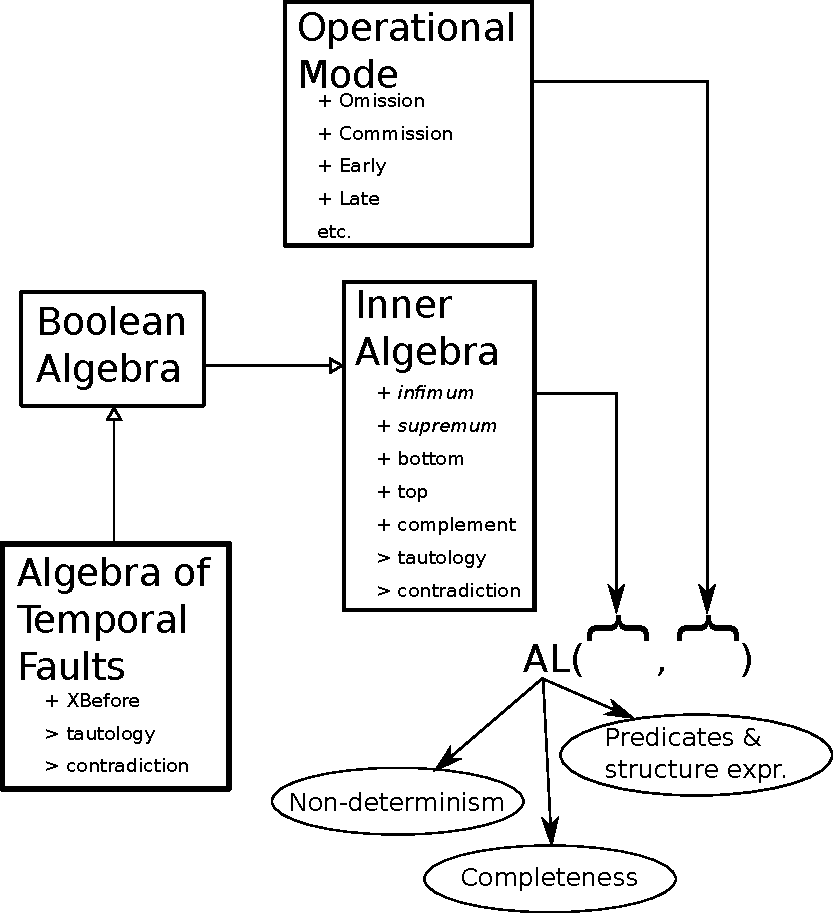
\includegraphics[width=0.6\textwidth]{logic-overview}
  \caption{\Ac{activation} overview}
  \label{fig:logic-overview}
\end{figure}

%Finally, structure expressions with order-related operators can be complex to analyse.
%Even to determine whether they are a contradiction or not~\cite{WP2009}.

%For example, what is the system behaviour when fault A occurs and then fault B occurs?
%What is a component behaviour when it detects a faulty behaviour in some of its inputs?
%Or, does the analyst considered all possibilities?
%Is there any erroneous behaviour case missing?

\begin{sloppypar}
We summarise the properties of \ac{activation} as follows:
%
\begin{enumerate}
  \item No expression predicate is a contradiction: there are no \emph{false} predicates in activation expressions;
  %\item There are no two terms that are \emph{active} simultaneously: only explicit non-determinism is allowed;
  \item The predicates in the terms of an expression consider all possible situations: expression tautology;
  \item There are no two terms with exactly the same operational mode: all expression terms are related to a unique operational mode.
\end{enumerate}
%
These properties form the \emph{healthiness conditions}~\cite{HH1998} of an expression in \ac{activation}.
\end{sloppypar}

We show the general form of \ac{activation} to model faults in \cref{sec:grammar}, the healthiness conditions to normalize expressions in \cref{sec:healthiness-conditions}, how to identify non-determinism in an expression in \cref{sec:non-determinism}, and the predicate notation to analyse systems and model fault propagation in \cref{sec:predicates-notation}.

\section[The Activation Logic Grammar]{The \acl*{activation} Grammar}
\label{sec:grammar}

Each term in \ac{activation} is a pair of a predicate and an operational mode.
The predicate is written in either Boolean algebra, \ac{algebra}, or any algebra that provides these properties: tautology and contradiction.
We assume that the set of possible faults on a system is finite and that each variable declared in a predicate represents a fault event.

The operational mode has two generic values: 
\begin{alineasinline}
  \item Nominal, and 
  \item Failure.
\end{alineasinline}
Nominal values either determine a value, or an undefined value (in this case, the constant value ``$\undefinednominal$'' is assumed).
Failure values denote an erroneous behaviour, which can be a total failure (for example, signal omission) or a failure that causes degradation (for example, a signal below or above its nominal range).
The choice of the operational modes depends on the system being analysed and its definition is generic and is left for the analyst.
For the \ac{activation}, it is sufficient to specify that it is an erroneous behaviour.

The grammar is parametrized by the syntax of an algebra (\verb|Algebra|) and a set of operational modes (\verb|OperModes|).
The initial rules of the grammar are defined as follows:
\begin{verbatim}
AL(Algebra, OperModes)     = TERM(Algebra, OperModes) 
                             | TERM(Algebra, OperModes) 
                               `|' AL(Algebra, OperModes)
TERM(Algebra, OperModes)   = `(' Algebra `,' OM(OperModes) `)'
OM(OperModes)              = `Nominal' NominalValue 
                             | `Failure' OperModes
NominalValue               = `undefined' | Number
Number                     = Integer | Bool | Decimal
\end{verbatim}
%
The denotational semantics of the expressions in \ac{activation} is a set of pairs.
The predicate in each term of an expression depends on the semantics of the inner algebra.
Thus the predicate evaluates to either \emph{true}~($\top$) or \emph{false}~($\bot$) depending on the valuation in the algebra.
In what follows we show a sketch of the denotational semantics of \ac{activation}.
%
\begin{align*}
  \logicInFormula{\left(P_1, O_1\right)} &\mapsto \{\left(P_1, O_1\right)\}\\
%%%%%%%%%%%%%%%%%%%%%%%%%%%%%%%%%%%%%%%%%%%%%%%%%%%%%%%%%%%%
  \logicInFormula{\left(P_1, O_1\right) | \left(P_2, O_2\right)} &\mapsto
    \{\left(P_1, O_1\right), \left(P_2, O_2\right)\}\\
%%%%%%%%%%%%%%%%%%%%%%%%%%%%%%%%%%%%%%%%%%%%%%%%%%%%%%%%%%%%
  \logicInFormula{Nominal~100} &\mapsto \Nominal{100}\\
%%%%%%%%%%%%%%%%%%%%%%%%%%%%%%%%%%%%%%%%%%%%%%%%%%%%%%%%%%%%
  \logicInFormula{Nominal~undefined} &\mapsto \Nominal{\undefinednominal}\\
%%%%%%%%%%%%%%%%%%%%%%%%%%%%%%%%%%%%%%%%%%%%%%%%%%%%%%%%%%%%
  \logicInFormula{Failure~Omission} &\mapsto \Failure{Omission}
\end{align*}
%
In an expression, if the $i^{th}$ predicate evaluates to $true$ ($\top$), we say that the $i^{th}$ operational mode is \emph{activated}.
To simplify the presentation of the expressions and to ease understanding, we use the denotational semantics in the remainder of this chapter (the right-hand side of the sketch above).
Thus, instead of using $\logicInFormula{Exp} = \logicInFormula{\left(P_1,O_1\right)} | \logicInFormula{\left(P_2,O_2\right)}$ we use $Exp = \left\{ \left(P_1,O_1\right), \left(P_2,O_2\right)  \right\}$

In this \lcnamecref{sec:grammar}, to illustrate the properties and possible analyses, we use an example of a system with faults $A$ and $B$ and the following outputs:
\begin{description}
  \item[$O_1$:] when $A$ is active;
  \item[$O_2$:] when $B$ is active;
  \item[$O_3$:] when $A$ is active, but $B$ is not;
  \item[$O_4$:] when $A$ or $B$ are active.
\end{description}
%
The expression for this example in \ac{activation} is:
\begin{equation}
S = \left\{\left(A, O_1\right), \left(B, O_2\right), \left(A \land \lnot B, O_3\right), \left(A \lor B, O_4\right)\right\}\label{eq:activation-example}
\end{equation}
%
We use \cref{eq:activation-example} in the following sections of this chapter to illustrate \ac{activation}.

In this example we see that one of the healthiness conditions is not satisfied: when, for instance, $A$ and $B$ are both inactive ($\lnot \left(A \land B\right)$), there is no explicit output defined.
%
In \cref{sec:activation-to-structure-expressions-algebra-operators} we show a more detailed case study to illustrate the reasoning about temporal faults.
In the next \lcnamecref{sec:healthiness-conditions}, we show how to normalise the expression, so that the three healthiness conditions are satisfied.

\section{Healthiness Conditions}
\label{sec:healthiness-conditions}

The healthiness conditions are fix points of a language.
The property is defined as a function of an expression and returns another expression.
For example, if a healthiness condition $\healthiness$ is satisfied by an expression $Exp$, we have $\healthinessfun{Exp} = Exp$.

In what follows we show the three healthiness conditions for \ac{activation}.
For convenience, we use the following abbreviations:
\begin{description}
  \item[contradiction:] the expression always evaluates to \emph{false};
  \item[tautology:] the expression always evaluates to \emph{true}.
\end{description}

\subsection[H1: No predicate is a contradiction]{$\healthiness[1]$: No predicate is a contradiction}
\label{sec:h1}

This property is very simple and it is used to eliminate any term that has a predicate that always evaluates to false.

\begin{definition}
Let $exp$ be an expression in \ac{activation}, then:
%
\begin{equation}
\healthinessfun[1]{exp} = \left\{~\left(P,O\right) ~|~ \left(P,O\right) \in exp \land \lnot \contradiction{P} ~\right\}
\end{equation}
%
where the operator $\in$ indicates that a term is present in the expression.
\end{definition}

Applying the first healthiness condition to our example results in:
\[\healthinessfun[1]{S} = S\]

Thus, we conclude that $S$ \emph{is} $\healthy[1]$.

\subsection[H2: All possibilities are covered]{$\healthiness[2]$: All possibilities are covered}
\label{sec:h2}

This property is used to make explicit that there are uncovered operational modes.
In this case, there is a combination of variables in the algebra that was not declared in the expression.
Very often the focus when modelling faults is on erroneous behaviour.
So we assume that such an uncovered operational mode is nominal, but has an undefined value.

\begin{definition}
Let $exp$ be an expression in the \ac{activation}, and $\tau$ is:
\[
\tau = \lnot \left (\bigvee_{\left(P,O\right)\in exp} P\right)
\]
%
then:
%
\begin{equation}
\healthinessfun[2]{exp} = 
  \begin{cases}
    exp, & \text{if } \contradiction{\tau}\\
    exp \cup \left\{\left(\tau,\Nominal{\undefinednominal}\right)\right\}, & \text{otherwise}
  \end{cases}
\end{equation}

\end{definition}

This property checks erroneous behaviour completeness. 
If the expression is already complete, all possibilities are already covered, and the expression is healthy.
Otherwise, a term containing the missing terms is introduced using the $\Nominal{\undefinednominal}.$

Applying the second healthiness condition to our example results in the following expression after simplification:
\[\healthinessfun[2]{S} = S \cup \left\{\left(\lnot A \land \lnot B, \Nominal{\undefinednominal}\right)\right\}\]

Thus, we conclude that $S$ \emph{is not} $\healthy[2]$.

\subsection[H3: There are no two terms with exactly the same operational mode.]{$\healthiness[3]$: There are no two terms with exactly the same operational mode}
\label{sec:h3}
This property merges terms that contain the same operational mode.
It avoids unnecessary formulas and may reduce the expression.

\begin{definition}
Let $exp$ be an expression in \ac{activation}. Then:
%
\begin{equation}
\label{eq:h3}
\begin{split}
\healthinessfun[3]{exp} = \left\{ \right.&\left(P_1, O_1\right) | \left(P_1, O_1\right) \in exp ~\land \\
    &\forall \left(P_2,O_2\right) \in exp \bullet 
      \left(P_1, O_1\right) = \left(P_2, O_2\right) \lor O_1 \neq O_2
  \left.\right\} \cup \\
  & \left\{ \left(P_1 \lor P_2, O_1\right) | \left(P_1, O_1\right),\left(P_2, O_2\right) \in exp \land O_1 = O_2 \right\}
\end{split}
\end{equation}
\end{definition}

Applying $\healthiness[3]$ in the example in the beginning of the \lcnamecref{chap:activation}, we conclude that $S$ \emph{is} $\healthy[3]$.
On the other hand, if we consider an $S'$ system being a copy of $S$, but making $O_1 = O_2$, then:
\[
\healthinessfun[3]{S'} = \left\{ 
  \left(A \lor B, O_1\right),
  \left(A \land \lnot B, O_3\right),
  \left(A \lor B, O_4\right)
\right\}
\]
Thus, we conclude that $S'$ \emph{is not} $\healthy[3]$.

\subsection{Healthy expression}
\label{sec:h}

To obtain a healthy expression, we apply all three healthiness conditions.
The order of application of each healthiness condition does not change the resulting expression.
The healthiness function is written as the composition of functions as follows:
\begin{equation}
\label{eq:h}
\healthiness = \healthiness[1] \circ \healthiness[2] \circ \healthiness[3]\end{equation}

After applying the three healthiness conditions to $S$, the resulting expression is:
\[
\begin{split}
\healthinessfun{S} = \left\{\right.
  & \left(A, O_1\right), \left(B, O_2\right),\\
  & \left(A \land \lnot B, O_3\right), \left(A \lor B, O_4\right),\\
  & \left(\lnot A \land \lnot B, \Nominal{undefined}\right)
\left.\right\}
\end{split}
\]

The healthiness conditions are useful to faults modelling, aiding the faults analyst to check contradictions and completeness.
Also, obtaining safe predicates is only possible in healthy expressions.
In the next \lcnamecref{sec:non-determinism}, we show how to verify non-determinism in \ac{activation} expressions.


\section{Non-determinism}
\label{sec:non-determinism}

Non-determinism is usually an undesirable property.
Thus, the analysis shall consider the activation of faults even if the fault might or not be active.

To identify non-determinism, we can check for the negation of a contradiction in a pair of predicates in the algebra.

\begin{definition}[Non-determinism]
\label{def:non-determinism}
Let $exp$ be an expression in \ac{activation}.

\begin{equation}
\label{eq:non-determinism}
\begin{split}
\nondet{exp} = &~ \exists \left(P_1,O_1\right),\left(P_2, O_2\right) \in exp~\bullet \\
  &~ \lnot \contradiction{P_1 \land P_2}
\end{split}
\end{equation}

\end{definition}

If there is at least one combination that evaluates $P_1 \land P_2$ to true (it is not a contradiction), then $exp$ is non-deterministic.
Our example is clearly non-deterministic as at least $A \land \left(A \lor B\right)$ is not a contradiction.

To analyse components and systems, and to model faults propagation, a predicate notation is shown in the next \lcnamecref{sec:predicates-notation}.
The predicate notation offers two additional ways to check non-determinism.

\section{Predicate Notation}
\label{sec:predicates-notation}

The \acl{activation} needs a special notation to enable the analysis of: 
\begin{alineasinline}
  \item a particular faults expression, or 
  \item a propagation in components.
\end{alineasinline}
Such a special notation extracts predicates in the algebra given an observable failure of the system (an undesired operational mode).

\begin{definition}[Predicate]
\label{def:predicate}
Let $exp$ be an expression in \ac{activation}, and $O_x$ an operational mode.
A predicate over $exp$ that matches $O_x$ is described as:
\begin{equation}
\label{eq:predicate}
\predicate{exp}{O_x} \iff \left.\exists \left(P, O\right) \in \healthinessfun{exp}\ \middle|\ O = O_x \bullet P\right.
\end{equation}
\end{definition}


The predicate notation function returns a predicate in the algebra.
For the example in the beginning of this \lcnamecref{sec:predicates-notation}, the predicate for $O_2$ is obtained as follows:
\[
\predicate{S}{O_2} = B
\]

To allow fault propagation of components we need another special notation. 
It expands the modes of an expression with a predicate in the inner algebra.

\begin{definition}[Modes]
Let $exp$ be an expression in \ac{activation}, and $P$ a predicate in the inner algebra, then:
\begin{equation}
\label{eq:modes}
\modes{exp}{P} = \left\{ \left(P_i \land P, O_i\right)\ \middle|\ (P_i, O_i) \in \healthinessfun{exp} \right\}
\end{equation}
%\begin{align*}
%\modes{S}{P} = &~ 
%	\left\{
%		\left(A \land P, O_1 \right), 
%		\left(B \land P, O_2 \right), 
%		\left(A \land \lnot B \land P, O_3 \right), 
%		\left(\left(A \lor B\right) \land P, O_2 \right)
%	\right\}
%\end{align*}

\end{definition}

Finally, to check the possible outputs, we need a function to obtain a set of outputs given an expression.

\begin{definition}[Activation]
\label{def:activation}
Let $exp$ be an expression in \ac{activation}, and $P_x$ a predicate in the inner algebra, then:

\begin{equation}
\label{eq:activation}
\activation{exp}{P_x} = \left\{
    O | (P, O) \in \healthinessfun{exp} \land \tautology{P_x \implies P}
  \right\}
\end{equation}

\end{definition}

Non-determinism can also be checked using the predicate notation and the activation property:
\begin{subequations}
\begin{align}
\activation{S}{A \land \lnot B} = &
  \left\{O_1, O_3\right\}\label{eq:s-nondet-activation}\\
\predicate{S}{O_1} \land 
  \predicate{S}{O_3} = & A \land \lnot B\label{eq:s-nondet-pred}
\end{align}
\end{subequations}
%
\Cref{eq:s-nondet-activation} shows that both $O_1$ and $O_3$ can be observed if $A \land \lnot B$ is \emph{true}. 
\Cref{eq:s-nondet-pred} states that if the possible operational modes of healthy $S$ are $O_1$ and $O_3$, then the predicate is $A \land \lnot B$.
Non-determinism is the possibility of observing two different failures ($O_1$ and $O_3$) for the same failure expression ($A \land \lnot B$) in the algebra.
In the next \lcnamecref{chap:case-study}, we show a practical case study using these properties and notations.



\chapter{Case study}
\label{chap:case-study}

\Embraer provided us with the \simulink model of an Actuator Control System (depicted in \cref{fg:acsBlockDiagrams}).
The failure expression of this system (that is, for each of its constituent components) was also provided by \embraer (we show some of them in \cref{tbl:acsAnnotations}).
In what follows we illustrate our strategy using the Monitor component.

A monitor component is a system commonly used for fault tolerance~\cite{ONB2002,KK2007}.
Initially, the monitor connects the main input (power source on input port 1) with its output.
It observes the value of this input port and compares it to a threshold.
If the value is below the threshold, the monitor disconnects the output from the main input and connects to the secondary input.
We present the \simulink model for this monitor in \cref{fg:blockDiagramMonitorInternals}.

%As we mentioned in~\cref{sec:faults-injection} we translated the monitor to \ac{CSPm} according to our strategy and modified the observer to make \acs{FDR} generate more counter-examples.

Sensors and actuators are used to improve safety by taking measures to decrease potential failures, as the leak protection system reported in~\cite{Andrews2001}, and shown in \cref{sec:probabilistic-analysis-non-coherent-tree}.
A sensor is installed in a room that may have gas leakage.
If the sensor detects a gas leak, then an actuator---a controlled valve---closes the gas flow.
A second valve diverts the gas flow if a high pressure is detected due the first valve closing.

Now we show five contributions:
\begin{alineasinline}
  \item using \ac{algebra}, but only with Boolean\index{Boolean Algebra} operators, thus ignoring ordering, we can obtain the same results obtained in~\cite{DM2012}, 
  \item representing each of the fault traces reported in~\cite{DM2012} as a term in our proposed \ac{algebra}, using the mapping function shown in \cref{sec:mapping-cspm-algebra},
  \item modelling faults of the monitor using \ac{activation}, using expressions in Boolean Algebra\index{Boolean Algebra}, 
  \item modelling faults of the monitor with \ac{activation}, but using \ac{algebra} as the inner algebra, and
  \item obtaining failure probability from a formula with explicit \ac{NOT} operators neither considering the consensus law nor the theory shown in~\cite{Andrews2001}.
\end{alineasinline}
%
Similarly to the association of fault events of \cref{tbl:acsAnnotations} in \cref{sec:faults-injection}, we associate the fault events as:
%
\begin{align*}
b_1 &= \text{LowPower-In1}& B_1 = \var b_1\\
b_2 &= \text{LowPower-In2}& B_2 = \var b_2\\
f &= \text{SwitchFailure}& F = \var f
\end{align*}
%
and for the leak detection system, we associate fault events as:
%
\begin{align*}
prv & = \text{the pressure relief valve fails} & PRV = \var{prv}\\
i_1 & = \text{there is an ignition source in room 1} &I_1 = \var{i_1}\\
l & = \text{there is a gas leak in room 1} & L = \var{l}\\
val & = \text{the isolation valve fails} & \VAL = \var{val}
\end{align*}

\section{From traces to structure expressions with Boolean operators}
\index{structure expression}
\label{sec:traces-to-structure-expressions-boolean-operators}

In this \lcnamecref{sec:traces-to-structure-expressions-boolean-operators} we show that the same result reported in~\cite{DM2012} in terms of static failure expression (or Boolean\index{Boolean Algebra} propositions) can be obtained with our Boolean\index{Boolean Algebra} operator without using \ac{XBefore}.
Similarly to the mapping function shown in \cref{sec:mapping-cspm-algebra}, we define a mapping function from traces to \ac{algebra} with Boolean operators only as:
%
\begin{subequations}
\begin{align}
\tracetobool{\trace{}} = & \top\label{eq:mapping-bool-empty}\\
%
\tracetobool{\trace{f}} = & \var{f}\label{eq:mapping-bool-singleton}\\
%
\tracetobool{\append{\trace{f_1}}{tr}} = & 
    \var{f_1} \land \tracetobool{tr}\label{eq:mapping-bool-two-more-trace}\\
%
\tracetobool{\left\{ tr_1, tr_2, \ldots, tr_n  \right\}} =& 
  \bigvee_{i \in \left\{1,\ldots,n\right\}} 
  \left(\tracetobool{tr_i} \land 
  \lnot \bigvee_{j \in \generators_{tr_i}} \var{f_j}\right)\label{eq:mapping-bool-set}
\end{align}
\end{subequations}
%
The only difference of the mapping function, when considering Boolean operators only, is \cref{eq:mapping-bool-two-more-trace}.
\Cref{eq:mapping-bool-set,eq:mapping-bool-singleton,eq:mapping-bool-empty} are identical to \cref{eq:mapping-algebra-set,eq:mapping-algebra-singleton,eq:mapping-algebra-empty}.

For each trace shown in \cref{sec:faults-injection}, the mapping function generates the following expressions
%
\begin{align*}
\text{\texttt{TRACE 1: }}&\tracetobool{\trace{f,b_2}} = F \land B_2 \\
\text{\texttt{TRACE 2: }}&\tracetobool{\trace{b_2,f}} = B_2 \land F \\
\text{\texttt{TRACE 3: }}&\tracetobool{\trace{b_1,b_2}} = B_1 \land B_2 \\
\text{\texttt{TRACE 4: }}&\tracetobool{\trace{b_2,b_1}} = B_2 \land B_1 \\
\text{\texttt{TRACE 5: }}&\tracetobool{\trace{b_1,f}} = B_1 \land F \\
\text{\texttt{TRACE 6: }}&\tracetobool{\trace{b_1,f,b_2}} = B_1 \land F \land B_2 \\
\text{\texttt{TRACE 7: }}&\tracetobool{\trace{b_1,b_2,f}} = B_1 \land B_2 \land F \\
\text{\texttt{TRACE 8: }}&\tracetobool{\trace{b_2,b_1,f}} = B_2 \land B_1 \land F \\
\text{\texttt{TRACE 9: }}&\tracetobool{\trace{f,b_1,b_2}} = F \land B_1 \land B_2 \\
\text{\texttt{TRACE 10: }}&\tracetobool{\trace{f,b_2,b_1}} = F \land B_2 \land B_1 \\
\text{\texttt{TRACE 11: }}&\tracetobool{\trace{b_2,f,b_1}} = B_2 \land F \land B_1 
\end{align*}

They represent the same faults shown in \cref{sec:faults-injection}.
%Note that the negation in the formula is very simple to represent in \ac{algebra} (and \ac{FBA}\index{Boolean Algebra!Free}) because it is just the absence of the generator.
%
By applying the mapping function, \cref{eq:mapping-bool-set}, for the previously shown set of traces, we obtain the following expression in \ac{algebra} (and in \ac{FBA}\index{Boolean Algebra!Free}):
%
\begin{equation}
M_{bool} = (B_1 \land B_2) \lor (F \land (B_1 \lor B_2))\label{eq:m-bool}
\end{equation}
%
which is equivalent to \possessiveembraer failure expression shown in \cref{tbl:acsAnnotations}.
%
This shows that \ac{algebra} can represent (static) failure expression as in our previous work~\cite{DM2012}.

\section{From traces to structure expressions with \acs*{XBefore}}
\label{sec:traces-to-structure-expressions-algebra-operators}
\index{structure expression}

Now, by using \ac{algebra} with the \ac{XBefore} operator and the mapping function shown in \cref{eq:mapping-algebra-empty,eq:mapping-algebra-singleton,eq:mapping-algebra-set,eq:mapping-algebra-two-more-trace}, we can capture each possible individual sequences as generated by the work~\cite{DM2012}:
%
\begin{align*}
\text{\texttt{TRACE 1: }}&\tracetoalgebra{\trace{f,b_2}} = \parsin{\xbefore{F}{B_2}}\\
\text{\texttt{TRACE 2: }}&\tracetoalgebra{\trace{b_2,f}} = \parsin{\xbefore{B_2}{F}}\\
\text{\texttt{TRACE 3: }}&\tracetoalgebra{\trace{b_1,b_2}} = \parsin{\xbefore{B_1}{B_2}}\\
\text{\texttt{TRACE 4: }}&\tracetoalgebra{\trace{b_2,b_1}} = \parsin{\xbefore{B_2}{B_1}}\\
\text{\texttt{TRACE 5: }}&\tracetoalgebra{\trace{b_1,f}} = \parsin{\xbefore{B_1}{F}}\\
\text{\texttt{TRACE 6: }}&\tracetoalgebra{\trace{b_1,f,b_2}} = 
  \xbefore{B_1}{\left(\xbefore{F}{B_2}\right)} \\
\text{\texttt{TRACE 7: }}&\tracetoalgebra{\trace{b_1,b_2,f}} = 
  \xbefore{B_1}{\left(\xbefore{B_2}{F}\right)} \\
\text{\texttt{TRACE 8: }}&\tracetoalgebra{\trace{b_2,b_1,f}} = 
  \xbefore{B_2}{\left(\xbefore{B_1}{F}\right)} \\
\text{\texttt{TRACE 9: }}&\tracetoalgebra{\trace{f,b_1,b_2}} = 
  \xbefore{F}{\left(\xbefore{B_1}{B_2}\right)} \\
\text{\texttt{TRACE 10: }}&\tracetoalgebra{\trace{f,b_2,b_1}} = 
  \xbefore{F}{\left(\xbefore{B_2}{B_1}\right)} \\
\text{\texttt{TRACE 11: }}&\tracetoalgebra{\trace{b_2,f,b_1}} = 
  \xbefore{B_2}{\left(\xbefore{F}{B_1}\right)} 
\end{align*}

Using the mapping function, \cref{eq:mapping-algebra-set}, for the previously shown set of traces, we obtain:
%
\begin{align}
M_A = & 
  \left(\xbefore{F}{B_2} \land \lnot B_1\right) \lor
  \left(\xbefore{B_2}{F} \land \lnot B_1\right) \lor
  \left(\xbefore{B_1}{B_2} \land \lnot F\right) \lor \nonumber \\
  & \left(\xbefore{B_2}{B_1} \land \lnot F\right) \lor
  \left(\xbefore{B_1}{F} \land \lnot B_2\right) \lor
  \left(\xbefore{B_1}{\left(\xbefore{F}{B_2}\right)}\right) \lor \nonumber \\
  &\left(\xbefore{B_1}{\left(\xbefore{B_2}{F}\right)}\right) \lor
  \left(\xbefore{B_2}{\left(\xbefore{B_1}{F}\right)}\right) \lor
  \left(\xbefore{F}{\left(\xbefore{B_1}{B_2}\right)}\right) \lor \nonumber \\
  &\left(\xbefore{F}{\left(\xbefore{B_2}{B_1}\right)}\right) \lor
  \left(\xbefore{B_2}{\left(\xbefore{F}{B_1}\right)}\right) \nonumber \\
%
  = & \left(F \land B_2 \land \lnot B_1\right) \lor 
  \left(B_1 \land B_2 \land \lnot F\right) \lor
  \left(\xbefore{B_1}{F} \land \lnot B_2\right) \lor \nonumber \\
  & \left(\xbefore{B_1}{\left(\xbefore{F}{B_2}\right)}\right) \lor 
  \left(\xbefore{B_1}{\left(\xbefore{B_2}{F}\right)}\right) \lor
  \left(\xbefore{B_2}{\left(\xbefore{B_1}{F}\right)}\right) \lor \nonumber \\
  & \left(\xbefore{F}{\left(\xbefore{B_1}{B_2}\right)}\right) \lor 
  \left(\xbefore{F}{\left(\xbefore{B_2}{B_1}\right)}\right) \lor
  \left(\xbefore{B_2}{\left(\xbefore{F}{B_1}\right)}\right) 
  & \text{by \cref{thm:xbefore-inf-1}} \nonumber \\
%
  = & \left(F \land B_2 \land \lnot B_1\right) \lor 
  \left(B_1 \land B_2 \land \lnot F\right) \lor
  \left(\xbefore{B_1}{F} \land \lnot B_2\right) \lor \nonumber \\
  & \left(B_2 \land \left(\xbefore{B_1}{F}\right)\right) \lor
  \left(B_2 \land \left(\xbefore{F}{B_1}\right)\right)
  & \text{by \cref{thm:and_xbefore_equiv_or_xbefore_expanded}} \nonumber \\
%
  = &\left(B_1 \land B_2\right) \lor \left(F \land B_2\right) \lor
    \left(\xbefore{B_1}{F} \land \lnot B_2\right) \label{eq:m-algebra}
\end{align}

The semantics of the above expression is:
\begin{alineasinline}
  \item fault $b_2$ ($\var{b_2}$) occurs and fault $b_1$ ($\var{b_1}$) or fault $f$ ($\var{f}$) occurs, or
  \item fault $b_1$ occurs before fault $f$ and fault $b_2$ does not occur, which is more precise than the expression found without considering order of events.
\end{alineasinline}

Expanding \cref{eq:m-bool}, we have:
\[
(B_1\land B_2) \lor (F \land B_2) \lor (F \land B_1)
\]
%
which differs from \cref{eq:m-algebra} only on terms: $F \land B_1$ (of $M_{bool}$) and $\xbefore{B_1}{F}\land \lnot B_2$ (of $M_A$).

\section[From AL to structure expressions with Boolean operators]{From \ac*{activation} to structure expressions with Boolean operators}
\label{sec:activation-to-structure-expressions-boolean-operators}

The power source has only two possible operational modes: 
\begin{alineasinline}
  \item the power source works as expected, providing a nominal value of $12V$, and 
  \item it has an internal failure $B_i$, and its operational mode is ``low power''.
\end{alineasinline}
%
In \ac{activation} it is modelled as:
\begin{equation}
\label{eq:power-source}
PowerSource_i = \left\{
  \left(B_i, LP\right),
  \left(\lnot B_i, \Nominal{12V}\right)
  \right\}
\end{equation}
%
where $LP$ is the LowPower failure.
$PowerSource_i$ is healthy:
\begin{itemize}
	\item $\healthy[1]$: there is no contradiction in the expressions;
	\item$\healthy[2]$: combining the expressions of the pairs in a disjunction, we obtain a tautology;
	\item$\healthy[3]$: the operational modes of the pairs are distinct.
\end{itemize}


The monitor is a bit different because its behaviour depends not only on internal faults, but also on its inputs. 
We now use the predicate notation defined in \cref{sec:predicates-notation} to express fault propagation.
As the monitor has two inputs and its behaviour is described in \cref{fg:blockDiagramMonitorInternals}, then it is a function of the expressions of both inputs:
%
\begin{equation}
\label{eq:monitor-bool}
\begin{split}
Monitor_{bool} &\left(in_1, in_2\right) = \\
  & \modes{in_1}{\predicate{in_1}{\Nominal{X}} \land \lnot F} \cup\\
  & \modes{in_2}{\lnot \predicate{in_1}{\Nominal{X}} \land \lnot F} \cup\\
  & \modes{in_2}{\predicate{in_1}{\Nominal{X}} \land F} \cup\\
  & \modes{in_1}{\lnot \predicate{in_1}{\Nominal{X}} \land F}
\end{split}
\end{equation}
where $X$ is an unbound variable and assumes any value.
%
The expression states the following:
\begin{itemize}
  \item The monitor output is the same as $in_1$ if the output of $in_1$ \emph{is} nominal and \emph{there is no} internal failure in the monitor:
  \[
  \modes{in_1}{\predicate{in_1}{\Nominal{X}} \land \lnot F}
  \]
  %%%%%%%%%%%%%%%%%%%%%%%%%%
  \item The monitor output is the same as $in_2$ if the output of $in_1$ \emph{is not} nominal and \emph{there is no} internal failure in the monitor:
  \[
  \modes{in_2}{\lnot \predicate{in_1}{\Nominal{X}} \land \lnot F}
  \]
  %%%%%%%%%%%%%%%%%%%%%%%%%%
  \item The monitor output is the converse of the previous two conditions if the internal failure $F$ is active:
  \[
  \begin{split}
  \modes{in_2}{\predicate{in_1}{\Nominal{X}} \land F} &\cup\\
  \modes{in_1}{\lnot \predicate{in_1}{\Nominal{X}} \land F} &
  \end{split}
  \]
\end{itemize}

The operational modes (observed behaviour) of the monitor depend on: 
\begin{alineasinline}
  \item its internal fault, and 
  \item propagated errors from its inputs.
\end{alineasinline}
%
Composing the monitor with the two power sources, we obtain the \ac{activation} expression of a power supply subsystem $System_{bool}$:
%
\begin{align*}
Sy&stem_{bool} = \\
 & Monitor_{bool} \left(PowerSource_1, PowerSource_2\right) \\
  = & \modes{in_1}{\lnot B_1 \land \lnot F} \cup
  \modes{in_2}{\lnot \lnot B_1 \land \lnot F} \cup\\
  & \modes{in_2}{\lnot B_1 \land F} \cup
  \modes{in_1}{\lnot \lnot B_1 \land F} & \text{by \cref{eq:predicate}}\\
  %%%%%%%%%%%%%%%%%%%%%%%%%%%%%%
  = &\modes{in_1}{\lnot B_1 \land \lnot F} \cup
  \modes{in_2}{ B_1 \land \lnot F} \cup\\
  &\modes{in_2}{\lnot B_1 \land F} \cup
  \modes{in_1}{B_1 \land F} & \text{by simplification}\\
%%%%%%%%%%%%%%%%%%%%%%%%%%%%%%%%%
  = & \left\{ \left(P_i \land \lnot B_1 \land \lnot F, O_i\right) | \left(P_i, O_i\right) \in in_1  \right\} \cup\\
  & \left\{ \left(P_i \land B_1 \land \lnot F, O_i\right) | \left(P_i, O_i\right) \in in_2  \right\} \cup\\
  & \left\{ \left(P_i \land \lnot B_1 \land F, O_i\right)| \left(P_i, O_i\right) \in in_2  \right\} \cup \\
  & \left\{ \left(P_i \land B_1 \land F, O_i\right)| \left(P_i, O_i\right) \in in_1 \right\} & \text{by \cref{eq:modes}}\\
%%%%%%%%%%%%%%%%%%%%%%%%%%%%%%%%%
  = & \left\{ 
      \left(B_1 \land \lnot B_1 \land \lnot F, LP\right), \right.\\
  &   \left(\lnot B_1 \land \lnot B_1 \land \lnot F, \Nominal{12V}\right), \\
  &   \left(B_2 \land B_1 \land \lnot F, LP\right),\\
  &   \left(\lnot B_2 \land B_1 \land \lnot F, \Nominal{12V}\right), \\
  &   \left(B_2 \land \lnot B_1 \land F, LP\right), \\
  &   \left(\lnot B_2 \land \lnot B_1 \land F, \Nominal{12V}\right),\\
  &   \left(B_1 \land B_1 \land F, LP\right), \\
  &   \left.\left(\lnot B_1 \land B_1 \land F, \Nominal{12V}\right)\right\}
    & \text{replacing vars}\\
\end{align*}

Simplifying and applying $\healthiness[1]$, we obtain:
%
\[
\begin{split}
\healthinessfun[1]{System_{\mathrm{bool}}} = &\\
  & \left\{ 
      \left(\lnot B_1 \land \lnot F, \Nominal{12V}\right), 
      \left(B_2 \land B_1 \land \lnot F, LP\right),\right.\\
  &   \left(\lnot B_2 \land B_1 \land \lnot F, \Nominal{12V}\right), 
      \left(B_2 \land \lnot B_1 \land F, LP\right), \\
  &   \left.\left(\lnot B_2 \land \lnot B_1 \land F, \Nominal{12V}\right),
      \left(B_1 \land F, LP\right)\right\}
\end{split}
\]

Applying, $\healthiness[3]$, we simplify to:
%
\[
\begin{split}
\healthiness[3] \circ \healthiness[1] &\left(System_{\mathrm{bool}}\right)\\
=  & \left\{ 
      \left(
        \begin{split}
          \left(\lnot B_1 \land \lnot F\right) \lor\\
          \left(B_1 \land \lnot B_2 \land \lnot F \right)\lor \\
          \left(\lnot B_1 \land \lnot B_2 \land F \right)
        \end{split},
        \Nominal{12V}
      \right),
    \right.\\
  & \left.
      \left(
        \begin{split}
        \left(B_1 \land B_2 \land \lnot F\right) \lor \\
        \left(\lnot B_1 \land B_2 \land F\right) \lor \\
        \left(B_1 \land F\right)
        \end{split}, 
        LP
      \right)
    \right\}\\
= & \left\{
    \left(\left(\lnot B_1 \land \lnot B_2\right) \lor 
      \lnot F \land \left(\lnot B_1 \lor \lnot B_2\right), 
      \Nominal{12V}\right), \right.\\
  & \left.  
    \left(F \land \left(B_1 \lor B_2\right) \lor \left(B_1 \land B_2\right), 
      LP\right)
  \right\}
\end{split}
\]

The monitor expression is $\healthy[2]$ (the predicates are complete), thus:
\[
\healthiness[2] \circ \healthiness[3] \circ \healthiness[1]\left(System_{\mathrm{bool}}\right) =
\healthiness[3] \circ \healthiness[1]  \left(System_{\mathrm{bool}}\right)
\]

The resulting expression for the monitor after applying all healthiness conditions is:
\begin{equation}
\label{eq:h-system1}
\begin{split}
  \healthinesscmd\left(System_{\mathrm{bool}}\right) = & \left\{
    \left(\left(\lnot B_1 \land \lnot B_2\right) \lor 
      \lnot F \land \left(\lnot B_1 \lor \lnot B_2\right), \Nominal{12V}\right),\right.\\
%%%%%%%%%%%%%
    &\left.\left(F \land \left(B_1 \lor B_2\right) \lor \left(B_1 \land B_2\right), LP\right)
  \right\}
\end{split}
\end{equation}
%
The operational modes of $System_{\mathrm{bool}}$ is either $\Nominal{12V}$ or $LP$ (low power).

Finally, we obtain the \emph{low power} structure expression (see \cref{tbl:acsAnnotations}) using the predicate notation:
\[
\predicate{System_{\mathrm{bool}}}{LP} \iff
F \land \left(B_1 \lor B_2\right) \lor \left(B_1 \land B_2\right)
\]

The monitor expression also indicates that if the switch is operational ($\lnot F$) and at least one PowerSource is operational ($\lnot B_1 \lor \lnot B_2$), the monitor output is nominal.
But if at least one PowerSource is faulty ($B_1 \lor B_2$) and the monitor has an internal failure ($F$) the system is not operational.
These two sentences---written in \ac{activation} using the predicate notation---are:
\begin{subequations}
\begin{align}
\activationcmd& \left(System_{\mathrm{bool}}, \lnot F \land \left(\lnot B_1 \lor \lnot B_2\right)\right) \nonumber\\
  = & \left\{ O | \left(P, O\right) \in \healthinesscmd\left(System_{\mathrm{bool}}\right) \land \right.\nonumber\\
    & \left.\tautology{\lnot F \land \left(\lnot B_1 \lor \lnot B_2\right) \implies P}
  \right\} & \text{[by \cref{eq:activation}]}\nonumber\\
  = & \left\{\Nominal{12V}\right\} & \text{[by simplification]}\\
%%%%%%%%%%%%%%%%%%%
\activationcmd& \left(System_{\mathrm{bool}}, F \land \left(B_1 \lor B_2\right) \right) \nonumber\\
  = & \left\{ O | \left(P, O\right) \in \healthinesscmd\left(System_{\mathrm{bool}}\right) \land \right.\nonumber\\
    & \left.\tautology{F \land \left(B_1 \lor B_2\right) \implies P}
  \right\} & \text{[by \cref{eq:activation}]}\nonumber\\
  = & \left\{LP\right\} & \text{[by simplification]}
\end{align}
\end{subequations}

\section[From AL to structure expressions with XBefore]{From \ac*{activation} to structure expressions with \ac*{XBefore}}
\label{sec:activation-to-structure-expressions-algebra-operators}

Now, let us consider the same system but with a subtle modification.
As shown in~\cite{DM2016}, the order of the occurrence of faults may be relevant, and the qualitative and quantitative analyses results may be different than those results without considering the order of the occurrence of faults.
Observing \cref{fg:blockDiagramMonitorInternals}, we see that if $F$ activates before a failure in the first input of the monitor, then it would display a nominal behaviour.
This is because the internal failure $F$ anticipates switching to the second input.
On the other hand, if the first input fails before $F$, then the monitor would switch to the second input, and then switch back due to the internal failure.
We obtain the following expression for the monitor, now using the \ac{algebra}:

%
\begin{equation}
\label{eq:monitor-algebra}
\begin{split}
Monitor_{XB} &\left(in_1, in_2\right) = \\
  & \modes{in_1}{\predicate{in_1}{\Nominal{X}} \land \lnot F} \cup\\
  & \modes{in_2}{\lnot \predicate{in_1}{\Nominal{X}} \land \lnot F} \cup\\
  & \modes{in_2}{\predicate{in_1}{\Nominal{X}} \land F} \cup\\
  & \modes{in_1}{\xbefore{\lnot \predicate{in_1}{\Nominal{X}}}{F}} \cup \\
  & \modes{in_2}{\xbefore{F}{\lnot \predicate{in_1}{\Nominal{X}}}}
\end{split}
\end{equation}
where $X$ is an unbound variable and assumes any value.

\begin{sloppypar}
The difference to $System_{\mathrm{bool}}$ (\cref{eq:monitor-bool}) is only the finer analysis of the cases of erroneous behaviours of the first input and an internal failure.
Note that the finer analysis splits the predicate 
%
\begin{align*}
  & \lnot \predicate{in_1}{\Nominal{12V}} \land F & \text{(activates } in_1\text{)}\\
  \intertext{into:}
  & \xbefore{\lnot\predicate{in_1}{\Nominal{12V}}}{F} & \text{(activates } in_1\text{)}\\
  \intertext{and}
  & \xbefore{F}{\lnot\predicate{in_1}{\Nominal{12V}}} & \text{(activates } in_2\text{)}
\end{align*}
%
We can assure that such a split is complete because the predicate notation evaluates to $B_1$. 
As the operands satisfy all temporal properties (\cref{def:tempo1,def:tempo2,def:tempo3,def:tempo4}) and events independence (\cref{law:independent-events}), thus the law shown in \cref{thm:xbefore-sup-equiv-inf} is valid.
For the first split item, the expected behaviour is the same as $in_1$ because the system switches to $in_2$, but then an internal failure occurs, and it switches back to $in_1$.
For the second split item, it switches to $in_2$ due to an internal failure, then the first input fails, so the behaviour is similar to the nominal behaviour (see the second \emph{modes} in \cref{eq:monitor-algebra}).
\end{sloppypar}
%
Following the similar expansions of \cref{eq:monitor-bool}, we obtain:
%
\begin{align*}
System_{XB} = & Monitor_{XB} \left(PowerSource_1, PowerSource_2\right) \\
%  = & \modes{in_1}{\lnot B_1 \land \lnot F} \cup\\
%  & \modes{in_2}{\lnot \lnot B_1 \land \lnot F} \cup\\
%  & \modes{in_2}{\lnot B_1 \land F} \cup\\
%  & \modes{in_1}{\xbefore{\lnot \lnot B_1}{F}} \cup\\
%  & \modes{in_2}{\xbefore{F}{\lnot \lnot B_1}} & \text{by \cref{eq:predicate}}\\
%%%%%%%%%%%%%%%%%%%%%%%%%%%%%%
%  = & \modes{in_1}{\lnot B_1 \land \lnot F} \cup
%   \modes{in_2}{B_1 \land \lnot F} \cup\\
%  & \modes{in_2}{\lnot B_1 \land F} \cup
%   \modes{in_1}{\xbefore{B_1}{F}} \cup\\
%  & \modes{in_2}{\xbefore{F}{B_1}} & \text{by simpl.}\\
%%%%%%%%%%%%%%%%%%%%%%%%%%%%%%%%%
%  = & \left\{ \left(P_i \land \lnot B_1 \land \lnot F, O_i\right) | \left(P_i, O_i\right) \in in_1  \right\} \cup\\
%  & \left\{ \left(P_i \land B_1 \land \lnot F, O_i\right) | \left(P_i, O_i\right) \in in_2  \right\} \cup\\
%  & \left\{ \left(P_i \land \lnot B_1 \land F, O_i\right)| \left(P_i, O_i\right) \in in_2  \right\} \cup \\
%  & \left\{ \left(P_i \land \xbefore{B_1}{F}, O_i\right)| \left(P_i, O_i\right) \in in_1 \right\} \cup\\
%  & \left\{ \left(P_i \land \xbefore{F}{B_1}, O_i\right)| \left(P_i, O_i\right) \in in_2 \right\} & \text{by \cref{eq:modes}}\\
%%%%%%%%%%%%%%%%%%%%%%%%%%%%%%%%%
  = & 
	\left\{ 
		\left(B_1 \land \lnot B_1 \land \lnot F, LP\right), 
		\left(\lnot B_1 \land \lnot B_1 \land \lnot F, \Nominal{12V}\right),
	\right.\\
	& 
	\left(B_2 \land B_1 \land \lnot F, LP\right),
	\left(\lnot B_2 \land B_1 \land \lnot F, \Nominal{12V}\right), \\
	& 
	\left(B_2 \land \lnot B_1 \land F, LP\right), 
	\left(\lnot B_2 \land \lnot B_1 \land F, \Nominal{12V}\right),\\
    &
    \left(B_1 \land \xbefore{B_1}{F}, LP\right),
    \left.\left(\lnot B_1 \land \xbefore{B_1}{F}, \Nominal{12V}\right)\right\}, \\
    & 
    \left.
	    \left(B_2 \land \xbefore{F}{B_1}, LP\right),
	    \left(\lnot B_2 \land \xbefore{F}{B_1}, \Nominal{12V}\right)
    \right\}
\end{align*}

Simplifying and applying $\healthiness[1]$ to remove contradictions, we obtain:
\begin{align*}
\healthinessfun[1]{System_{XB}} = &\\
  & \left\{ 
      \left(\lnot B_1 \land \lnot F, \Nominal{12V}\right), 
      \left(B_2 \land B_1 \land \lnot F, LP\right),\right.\\
  &   \left(\lnot B_2 \land B_1 \land \lnot F, \Nominal{12V}\right), 
      \left(B_2 \land \lnot B_1 \land F, LP\right), \\
  &   \left(\lnot B_2 \land \lnot B_1 \land F, \Nominal{12V}\right),
      \left(\xbefore{B_1}{F}, LP\right), \\
  &   \left.\left(B_2 \land \xbefore{F}{B_1}, LP\right), 
      \left(\lnot B_2 \land \xbefore{F}{B_1}, \Nominal{12V}\right) \right\}
\end{align*}

Applying $\healthiness[3]$ to remove redundant terms with identical operational modes and using the rules shown in \cref{sec:xbefore-laws}, we simplify to:
\[
\begin{split}
\healthiness[3] \circ \healthiness[1] &\left(System_{XB}\right)\\
=  & \left\{ 
      \left(
        \begin{split}
          \left(\lnot B_1 \land \lnot F\right) \lor\\
          \left(B_1 \land \lnot B_2 \land \lnot F \right)\lor \\
          \left(\lnot B_1 \land \lnot B_2 \land F \right)\lor \\
          \left(\lnot B_2 \land \xbefore{F}{B_1}\right)
        \end{split},
        \Nominal{12V}
      \right),
      \left(
        \begin{split}
        \left(B_1 \land B_2 \land \lnot F\right) \lor \\
        \left(\lnot B_1 \land B_2 \land F\right) \lor \\
        \left(\xbefore{B_1}{F}\right) \lor \\
        \left(B_2 \land \xbefore{F}{B_1}\right)
        \end{split}, 
        LP
      \right)
    \right\}\\
=  & \left\{ 
      \left(
        \begin{split}
          \left(\lnot B_1 \land \lnot F\right) \lor\\
          \left(B_1 \land \lnot B_2 \land \lnot F \right)\lor \\
          \left(\lnot B_1 \land \lnot B_2 \land F \right)\lor \\
          \left(\lnot B_2 \land \xbefore{F}{B_1}\right)
        \end{split},
        \Nominal{12V}
      \right),
      \left(
        \begin{split}
        \left(B_1 \land B_2 \land \lnot F\right) \lor \\
        \left(\lnot B_1 \land B_2 \land F\right) \lor \\
        \left(B_2 \land \xbefore{B_1}{F}\right) \lor \\
        \left(\lnot B_2 \land \xbefore{B_1}{F}\right) \lor\\
        \left(B_2 \land \xbefore{F}{B_1}\right)
        \end{split}, 
        LP
      \right)
    \right\}\\
%=  & \left\{ 
%      \left(
%        \begin{split}
%          \left(\lnot B_1 \land \lnot F\right) \lor\\
%          \left(B_1 \land \lnot B_2 \land \lnot F \right)\lor \\
%          \left(\lnot B_1 \land \lnot B_2 \land F \right)\lor \\
%          \left(\lnot B_2 \land \xbefore{F}{B_1}\right)
%        \end{split},
%        \Nominal{12V}
%      \right),
%    \right.\\
%  & \left.
%      \left(
%        \begin{split}
%        \left(B_1 \land B_2 \land \lnot F\right) \lor \\
%        \left(\lnot B_1 \land B_2 \land F\right) \lor \\
%        \left(B_2 \land \xbefore{B_1}{F}\right) \lor \\
%        \left(\lnot B_2 \land \xbefore{B_1}{F}\right) \lor \\
%        \left(B_2 \land \xbefore{F}{B_1}\right)
%        \end{split}, 
%        LP
%      \right)
%    \right\}\\
%=  & \left\{ 
%      \left(
%        \begin{split}
%          \left(\lnot B_1 \land \lnot F\right) \lor\\
%          \left(B_1 \land \lnot B_2 \land \lnot F \right)\lor \\
%          \left(\lnot B_1 \land \lnot B_2 \land F \right)\lor \\
%          \left(\lnot B_2 \land \xbefore{F}{B_1}\right)
%        \end{split},
%        \Nominal{12V}
%      \right),
%    \right.\\
%  & \left.
%      \left(
%        \begin{split}
%        \left(B_1 \land B_2 \land \lnot F\right) \lor \\
%        \left(\lnot B_1 \land B_2 \land F\right) \lor \\
%        \left(\lnot B_2 \land \xbefore{B_1}{F}\right) \lor \\
%        \left(B_2 \land F \land B_1\right)
%        \end{split}, 
%        LP
%      \right)
%    \right\}\\
& = \left\{
    \left(\left(\lnot B_1 \land \lnot B_2\right) \lor 
      \lnot F \land \left(\lnot B_1 \lor \lnot B_2\right) \lor \right. 
      \lnot B_2 \land \xbefore{F}{B_1}, \Nominal{12V}\right), \\
  & \left.  
    \left(\left(B_1 \land B_2\right) \lor \left(B_2 \land F\right) \lor \left(\lnot B_2 \land \xbefore{B_1}{F}\right), 
      LP\right)
  \right\}
\end{split}
\]

\begin{sloppypar}
The monitor expression is $\healthy[2]$. 
Simplifying Boolean\index{Boolean algebra} operators as usual, the XBefore expression is:
%
\begin{align*}
  \left(\lnot B_2 \land \xbefore{F}{B_1}\right) &\lor \left(\lnot B_2 \land \xbefore{B_1}{F}\right)\\
  \intertext{which simplifies to}
  \lnot B_2 ~\land ~&~ F \land B_1 & \text{by \cref{thm:xbefore-sup-equiv-inf}}
\end{align*}
%
Thus:
\[
\healthiness[2] \circ \healthiness[3] \circ \healthiness[1]\left(System_{XB}\right) =
\healthiness[3] \circ \healthiness[1]  \left(System_{XB}\right)
\]
  
\end{sloppypar}

The resulting expression for the monitor after applying all healthiness conditions is:
\begin{equation}
\label{eq:h-systemalgebra}
\begin{split}
  \healthinesscmd\left(System_{XB}\right) = & \left\{
    \left(\left(\lnot B_1 \land \lnot B_2\right) \lor 
      \lnot F \land \left(\lnot B_1 \lor \lnot B_2\right) \lor \right.\right.\\
  & \left. \lnot B_2 \land \xbefore{F}{B_1}, \Nominal{12V}\right), \\
  & \left(\left(B_1 \land B_2\right) \lor \left(B_2 \land F\right) \lor \right.\\
  & \left.\left. \left(\lnot B_2 \land \xbefore{B_1}{F}\right), 
      LP\right)
  \right\}
\end{split}
\end{equation}

Finally, we obtain the \emph{low power} structure expression of the monitor using the predicate notation:
\[
\predicate{System_{XB}}{LP} \iff 
  \left(B_1 \land B_2\right) \lor 
  \left(B_2 \land F\right) \lor
  \left(\lnot B_2 \land \xbefore{B_1}{F}\right)
\]
%
Thus, $System_{XB}$ fails with $LP$ if:
\begin{itemize}
  \item Both power sources fail;
  \item The monitor fails to detect the nominal state of the first power source and the second power source is in a failure state;
  \item The monitor fails to detect the failure state of the first power source (the monitor fails after the failure of the first power source).
\end{itemize}
%
Note that if the monitor fails before the failure of the first power source, it fails to detect the operational mode of the first power source and switches to the second power source, which is in a nominal state (see expression $\lnot B_2 \land \xbefore{F}{B_1}$ in \cref{eq:h-systemalgebra}).

\section[Obtaining top-event probability with explicit NOT operators]{Obtaining top-event probability with explicit \ac*{NOT} operators}
\label{sec:top-event-probability-explicit-not}

In this \lcnamecref{sec:top-event-probability-explicit-not} we show how to use \ac{algebra} to obtain the same probability formula of \cref{eq:leak-protection-system-probability}.

We use \cref{eq:formula-probability-of-inf} to split the calculations of the top-event structure expression shown in \cref{eq:leak-protection-system-structure-expression}:
\begin{align}
\formulaprob{L \land 
  \left( \left(\lnot \VAL \land PRV\right) \lor 
  \left(\VAL \land I_1\right) \right) } = \nonumber\\
  \formulaprob{L} \times 
  \formulaprob{\left(\lnot \VAL \land PRV\right) \lor 
    \left(\VAL \land I_1\right)}\label{eq:leak-protection-system-split}
\end{align}

Then, we obtain the formula probability of the top-event probability of the structure expression shown in \cref{eq:leak-protection-system-structure-expression} in \ac{algebra}:
%
\begin{subequations}
\begin{align}
\formulaprob{L} = &~ \denotationalprob{\listsin{l}} & \text{by \cref{eq:formula-probability-any-generators}}\nonumber\\
= &~ P_l(t)\label{eq:leak-protection-system-top1}\\
%%%%%
\formulaprobop\{\left(\lnot \VAL \land PRV\right) \lor &\nonumber\\
    \left(\VAL \land I_1\right)\} = &~
    \denotationalprob{\listsin{prv}} + 
    \denotationalprob{\listsin{i_1,prv}} +  \nonumber\\
    &~\denotationalprob{\listsin{prv,i_1}} + 
    \denotationalprob{\listsin{val,i_1}} + \nonumber\\
    &~\denotationalprob{\listsin{i_1,val}} + \nonumber\\
    &~\denotationalprob{\listsin{val,i_1,prv}} + 
    \ldots + \nonumber\\
    &~\denotationalprob{\listsin{prv,i_1,val}} \nonumber
%%%%%
\intertext{Note that we use the expression without the consensus law, but the ``missing'' term $PRV \land I_1$ appears naturally on the denotational semantics used in our proposed probability calculation.}
%%%%%
\formulaprobop\{\left(\lnot \VAL \land PRV\right) \lor &\nonumber\\
    \left(\VAL \land I_1\right)\} = &~
    P_{prv}(t) \times (1 - P_{i_1}(t)) \times (1 - P_{val}(t)) \nonumber\\
    &~ P_{i_1}(t) \times P_{prv}(t) \times (1 - P_{val}(t)) \nonumber\\
    &~ P_{val}(t) \times P_{i_1}(t) \times (1 - P_{prv}(t)) \nonumber\\
    &~ P_{val}(t) \times P_{i_1}(t) \times P_{prv}(t) \nonumber\\
%%%%%
= &~ P_{prv}(t) + P_{val}(t) \times P_{i_1}(t) - P_{prv}(t) \times P_{val}(t)\label{eq:leak-protection-system-top2}
\end{align}
\end{subequations}

From \cref{eq:leak-protection-system-split,eq:leak-protection-system-top1,eq:leak-protection-system-top2}, we obtain:
\begin{equation}
\formulaprob{TOP} = P_l(t) \times \left(P_{prv}(t) + P_{val}(t) \times P_{i_1}(t) - P_{prv}(t) \times P_{val}(t)\right)
\end{equation}
%
which is equivalent to ~\cref{eq:leak-protection-system-probability}.




\chapter{Conclusion}
\label{sec:conclusion}

%In this work we presented a foundational theory to support a more precise representation of fault events as compared to our previous strategy for injecting faults~\cite{DM2012}.
%
%The failure expression is essential for system safety assessment because it is used as basic input for building \aclp{FT}~\cite{PMS+2001,JMS+2011,GMS+2010}.
%
%We use \simulink as starting point because it is a standard tool in the control systems industry.
%
%Furthermore, we still connect the strategy presented in~\cite{MJG+2010} with the works reported in~\cite{JMS+2011} (functional analysis) and in~\cite{GMS+2010,PMS+2001} (safety assessment) because our new algebra is at least a Boolean\index{Boolean Algebra} algebra.

%\begin{sloppypar}
%The work reported in~\cite{Walker2009,WP2009,WP2010} tackles simultaneity with ``nearly simultaneous'' events~\cite{EWG2013}.
%But we consider instantaneous events, like the work reported in~\cite{MRL2014}, because we assume that simultaneity is probabilistically impossible.
%\end{sloppypar}

%%%%%%%%%%%%%%%%%%%%%%%%%%%%%%ISF 


In this work we presented a foundational theory to support a more precise representation of fault events as compared to our previous strategy for injecting faults~\cite{DM2012}.
%
The failure logic is essential for system safety assessment because it is used as basic input for building fault trees~\cite{PMS+2001,JMS+2011,GMS+2010}.
%
%We use \simulink as starting point because it is a standard tool in the control systems industry.
%
Furthermore, we still connect the strategy presented in~\cite{MJG+2010} with the works reported in~\cite{JMS+2011} (functional analysis) and in~\cite{GMS+2010,PMS+2001} (safety assessment) because our new algebra is at least a Boolean algebra.

We also proposed a parametrized logic, the \ac{activation}, that enables the analysis of systems depending on the expressiveness of a given algebra and a given set of operational modes.
If \ac{algebra} is used as a parameter, then the order of occurrence of faults can be considered.
Other algebras, like ternary algebras \cite{Jones2016} can be used, since they have tautology and contradiction properties.
Although the \ac{activation} is not as detailed as \ac{AADL}, the predicate notation in conjunction with the \ac{algebra} provides a richer assertion framework.
Also, it is possible to verify non-determinism on the model, by: 
\begin{alineasinline}
  \item verifying its existence with the $\nondetcmd$ function, 
  \item providing an expression and obtaining the possible operational modes with the $\activationcmd$ function, or 
  \item using the predicate notation to obtain a predicate that enables two or more operational modes.
\end{alineasinline}


%A related approach to analyse a system behaviour is to employ passive testing. 
%In such an approach, a formalised tester supervises a system during its execution.
%Although testing is very important to the analysis of systems' behaviour, static fault analysis, even with dynamic fault trees, is different. 
%The traces that we extract from the model are traces without faults repetition that causes an unwanted behaviour. 
%For example, the work reported in \cite{BCN+2005} shows the analysis of invariants. 
%Such invariants are the observation of inputs and outputs in a specific order. 
%In our work, we consider that different order of fault events may or may not cause failures and that Boolean algebra is not sufficient to express such cases.

%The work reported in~\cite{Huffm2010} was used as a basis for all proofs.
%
%It contains a complete theory of Free Boolean Algebras, including a homomorphism from an FBA to any Boolean algebra.
%
%Proving that there is also a homomorphism from \algebra to any Boolean algebra is left as future work.

\begin{sloppypar}
	The work reported in~\cite{Walker2009,WP2009,WP2010} tackles simultaneity with ``nearly simultaneous'' events~\cite{EWG2013}.
	But we consider instantaneous events, like the work reported in~\cite{MRL2014}, because we assume that simultaneity is probabilistically impossible.
\end{sloppypar}
%Another future To show the relation of the exclusive before operator to the operators shown in~\cite{MRL2014} and~\cite{WP2009}.

%As future work we will complete the analysis including verification of a formula acceptance criteria.
%
%The objective of finding failure logic is to create fault trees and then performing qualitative and quantitative analyses to check if the fault trees meet safety requirements (for static and dynamic fault trees).
%
%We plan to verify safety requirements directly from the failure logic expressed by our TFA.
%
%It means we need a reduction technique that includes the exclusive before operator to analyse large-scale systems (say with 1000 or more fault events) without using dependency trees~\cite{WP2010}.
%
%We believe that the direct analysis on failure logic expressed by our TFA can also accelerate temporal fault trees analysis as it is a subclass of dynamic fault trees.

The distinct lists representation in our algebra does not allow obtaining minimal cut sequences directly from the formula, similar to \acp{FBA}.
The sets in \iac{FBA} formula are already the minimal cut sets.
In our work, \ac{algebra} allows us to find minimal cut sequences (with \ac{XBefore}) from the formulas in \ac{DNF} algebraically: each sub-expression is a minimal cut sequence.

Boolean formulas reduction can be achieved by: 
\begin{alineasinline}
  \item application of Boolean laws, 
  \item \acp{BDD}, or 
  \item \acp{FBA}.
\end{alineasinline}
%
We used Boolean and \ac{XBefore} laws to reduce \ac{algebra} formulas.
%
The work reported in~\cite{TXD2011,XTD2012} uses Sequential BDDs to reduce formulas with order-based operators.
%
We plan to use similar concepts in a future work.
A ternary tree with special nodes seems to be a solution, but we have not verified yet.

The works reported in~\cite{Merle2010,MRL+2010,MRL2011,Walker2009,WP2009} removed the \ac{NOT} operator.
Thus, the algebras defined there (to analyse \ac{TFT} and \ac{DFT}) resembles a Boolean algebra, but are not complete. 
The \ac{algebra} allows such trees to have \ac{NOT} operators and the analysis could be performed similarly to \ac{SFT}.
Compared to \acp{TFT}, \ac{algebra} does not allow simultaneous events.
Compared to \acp{DFT}, \ac{algebra} is equivalent to the algebra shown in the works reported in~\cite{MRL2011b,Merle2010}, although their algebra has an operator to represent simultaneity, because simultaneity is probabilistically impossible.
The inclusion of an operator to represent simultaneity and the proofs of relation of \ac{algebra} to the algebras of \ac{TFT} and \ac{DFT} are left as future work.

%%%%%%%%%%%%%%%%%%%%%%%%%%%%%%%%%%

%%%%%%%%%%%%%%%%%%%%%%%%%%%%% AISC
The \ac{AADL} is extensible. 
The work reported in~\cite{SAEAS55061A} shows an extension to perform dependability analysis through state machines and expressions on fault events and operational modes.
Although such an extension captures system behaviour, operational mode activation conditions are expressed in state transitions in combination with an extension of Boolean expressions (not related to order).
Our work relates operational modes and fault occurrences order explicitly.

As presented in~\cite{DM2016}, \acp{TFT} and \acp{DFT} structure expressions can be written as formulas in \ac{algebra}.
As the root events of \acp{TFT} and \acp{DFT} represent operational modes of a system, the \ac{algebra} can be used to associate root events with operational modes, thus allowing the combination of two or more fault trees.

Although the properties of \ac{activation} require that the inner algebra provides tautology and contradiction, and we used \ac{algebra} in the case study, we did not show tautology and contradiction for \ac{algebra}. 
Instead, we used a law to reduce the \ac{algebra} expression to a Boolean expression.
The methodology to check tautology and contradiction in \ac{algebra} is related to expression reduction, which is a future work.

The original expression shown in the case study (\cref{sec:activation-to-structure-expressions-algebra-operators}) was already $\healthy[2]$.
The second healthiness condition about completeness uses the concept of undefined value to make any expression $\healthy[2]$.
Algebraically it is fine, but in practice, the property should be met initially, thus the initial expression is already $\healthy[2]$.
This property should only be used as an alert to the analyst if it not met initially.

\section{Future work}

The use of Isabelle/HOL gave us a peace of mind to assure our results.
Using it, however, requires so much time to get used to the notation, and understand proof mechanisation.
%Some proofs of laws and theorems were left out of this work.
All laws shown in \cref{sec:temporal-properties,sec:xbefore-laws} were proved and are presented in \cref{app:formal-proofs-isabelle-hol}.
We plan to prove the other theorems related to probabilities and \ac{MCSeq} acceptance criteria verification.
Properties of the probability calculation of a formula needs to be proved as well.

Another future work is to relate \ac{algebra} with the algebras shown in~\cite{Merle2010,Walker2009}.
It is important because we can benefit from their results.
The main challenge is to define how to express simultaneity in \ac{algebra}, or, at least, how to map from \ac{algebra} to the other algebras.

Contradiction and tautology are verified using a structural reduction. 
For Boolean\index{Boolean algebra} algebras, \iac{BDD} is used.
A ternary tree with special nodes seems to be a solution, but needs investigation.

%%%%%%%%%%%%%%%%%%%%%%%%%%%%%%

%\section{Future work}

%The \distinctlists representation in our algebra does not allow obtaining minimal cut sequences\index{Minimal Cut!Sequences} directly from the formula, similar to \acp{FBA}\index{Boolean Algebra!Free}.
%The sets in \iac{FBA}\index{Boolean Algebra!Free} formula are already the minimal cut sets\index{Minimal Cut!Sets}.
%In our work, \ac{algebra} allows us to find minimal cut sequences\index{Minimal Cut!Sequences} (with XBefore) from the formulas in \ac{DNF} algebraically: each sub-expression is a minimal cut sequence\index{Minimal Cut!Sequences}.

%Boolean\index{Boolean Algebra} formulas reduction can be achieved by:
%\begin{alineasinline}
%  \item application of Boolean laws,
%  \item \ac{BDD}\index{Binary Decision Diagrams}, or
%  \item \acp{FBA}\index{Boolean Algebra!Free}.
%\end{alineasinline}
%We used Boolean\index{Boolean Algebra} and \ac{XBefore} laws to reduce \ac{algebra} formulas.
%%
%The work reported in~\cite{TXD2011,XTD2012} uses Sequential BDDs\index{Binary Decision Diagrams!Sequential} to reduce formulas with order-based operators.
%%
%We plan to use similar concepts in a future work.

%The work reported in~\cite{SAE1996b} states that \acp{DTMC} (\aca{DTMC}) is more appropriate to represent several states than \acp{SFT}.
%Considering that \acp{DFT} were conceived as a visual representation of \acap{DTMC}, then we may say that \acp{DFT} can be used to represent several states.
%Thus they are suitable to propose the architectural model modifications as shown in \cref{fig:strategy-overview}.
%The definition and the theory of ``Fault Modelling and Fault Tolerance Patterns'' and the automatic proposal of ``Architectural Model Modifications'' blocks are left as future work.




% References
\postextual
%\begin{references}
  \bibliography{references-jabref}
%\end{references}

% Appendix

%\theappendix
\begin{apendicesenv}
\partapendices

%\section{Formal proofs in Isabelle/HOL}
\chapter{Formal proofs in Isabelle/HOL}
\label{app:formal-proofs-isabelle-hol}

In the following we list all theorems and proofs concerning the laws presented in \cref{chap:algebra}.
The complete set of verifiable theory files is available at \algebraurl.
We list only those files created in our work.
Each theorem, proof or corollary is followed by its own proof.

The theory about lists of distinct elements (\distinctlists) is available in~\cite{HL2016} (we used the 2015 version that is available with \isabellehol).

%\Cref{tbl:laws-theorems-slice} shows a mapping of the equations shown in~\cref{chap:algebra} and theorem names in the \isabellehol code presented in this \namecref{app:formal-proofs-isabelle-hol}.

%\begin{table}[htb]
%  \caption{Laws and theorems}%
%  \label{tbl:laws-theorems-slice}%
%  \begin{longtable}{p{8cm}ll}
%    \hline
%    Description & Def. or Law & Theorem name \\
%    \hline \hline
%    \endfirsthead
%    \multicolumn{3}{c}%
%    {\tablename\ \thetable\ -- \textit{Continued from previous page}} \\
%    \hline
%    Description & Def. or Law & Theorem name \\
%    \hline
%    \endhead
%    \hline \multicolumn{3}{r}{\textit{Continued on next page}} \\
%    \endfoot
%    \hline
%    \endlastfoot
%    & \Cref{def:xbefore-append} & \\
%    \hline
    %Definition of slice in \distinctlists & \Cref{def:slice} & instantiation dlist, $l\dagger i..f$\\
%    \hline
%    Definition of slice-right & \Cref{def:slice-right} & slice\_right\\
%    \hline
%    Definition of slice-left & \Cref{def:slice-left} & slice\_left\\
%    \hline
    %Relation of slice and concatenation (appending) & \Cref{law:slice-append} &  slice\_append\\
%    \hline
    %Definition of \ac{XBefore} using slice & \Cref{def:xbefore-slice} &  dlist\_xbefore\_append\\
%    \hline
%    Variable definition & \Cref{def:var} & \\
%    \hline
%    & \Cref{def:algebraset-var} & \\
%    \hline
%    & \Cref{def:algebraset-compl} & \\
%    \hline
%    & \Cref{def:algebraset-inf} & \\
%    \hline
%    & \Cref{def:algebraset-xbefore} & \\
%    \hline
%    & \Cref{def:algebraset-true} & \\
%    \hline
%    & \Cref{def:algebraset-false} & \\
%    \hline
%    & \Cref{def:algebraset-sup} & \\
%    \hline
%    & \Cref{eqs:generators-independence} & \\
%    \hline
%    & \Cref{def:tempo1} & \\
%    \hline
%    & \Cref{def:tempo2} & \\
%    \hline
%    & \Cref{def:tempo3} & \\
%    \hline
%    & \Cref{def:tempo4} & \\
%    \hline
%    & \Cref{law:var-tempo} & \\
%    \hline
%    & \Cref{law:old-xbefore} & \\
%    \hline
%    & \Cref{law:tempo1-inter} & \\
%    \hline
%    & \Cref{law:tempo3-inter} & \\
%    \hline
%    & \Cref{law:tempo2-union} & \\
%    \hline
%    & \Cref{law:tempo4-union} & \\
%    \hline
%    & \Cref{law:independent-events} & \\
%    \hline
%    & \Cref{thm:xbefore-of-false-1} & \\
%    \hline
%    & \Cref{thm:xbefore-of-false-2} & \\
%    \hline
%    & \Cref{thm:xbefore-sup-absorb-1} & \\
%    \hline
%    & \Cref{thm:xbefore-sup-absorb-2} & \\
%    \hline
%    & \Cref{thm:xbefore-not-idempotent} & \\
%    \hline
%    & \Cref{thm:xbefore-associativity} & \\
%    \hline
%    & \Cref{thm:xbefore-inf-equiv-bot} & \\
%    \hline
%    & \Cref{thm:xbefore-sup-equiv-inf} & \\
%    \hline
%    & \Cref{thm:xbefore-sup-1} & \\
%    \hline
%    & \Cref{thm:xbefore-sup-2} & \\
%    \hline
%    & \Cref{thm:xbefore-inf-1} & \\
%    \hline
%    & \Cref{thm:xbefore-inf-2} & \\
%    \hline
%    & \Cref{thm:and_xbefore_equiv_or_xbefore} & \\
%    \hline
%    & \Cref{thm:and_xbefore_equiv_or_xbefore_expanded} & \\
%    \hline
%  \end{longtable}%
%\end{table}

This \namecref{app:formal-proofs-isabelle-hol} is organized as follows:
\begin{alineasinline}
  \item \cref{sec:theory-sliceable} presents the base lemmas and theorems for sliceable types;
  \item sublists (sliceable \distinctlists) are shown in \cref{sec:theory-sliceable-dlist};
  \item algebraic definitions and laws of the \ac{algebra} are shown in \cref{sec:theory-algebra}, and
  \item proofs using the denotational semantics of sets of \distinctlists are shown in \cref{sec:theory-algebra-dlist}.
\end{alineasinline}

%
\begin{isabellebody}%
\setisabellecontext{Sliceable}%
%
\isamarkupsection{Sliceable%
}
\isamarkuptrue%
%
\begin{isamarkuptext}%
\label{sec:theory-sliceable}%
\end{isamarkuptext}\isamarkuptrue%
%
\isadelimtheory
%
\endisadelimtheory
%
\isatagtheory
%
\endisatagtheory
{\isafoldtheory}%
%
\isadelimtheory
%
\endisadelimtheory
%
\begin{isamarkuptext}%
In this section we present a class to express sub-structures for a data type, and laws over such a class.
  For example, for lists, \emph{sliceable} defines operators and theorems to obtain sublists.%
\end{isamarkuptext}\isamarkuptrue%
\isacommand{class}\isamarkupfalse%
\ sliceable\ {\isacharequal}\ \isanewline
\ \ \isakeyword{fixes}\ slice\ {\isacharcolon}{\isacharcolon}\ {\isachardoublequoteopen}{\isacharprime}a\ {\isasymRightarrow}\ nat\ {\isasymRightarrow}\ nat\ {\isasymRightarrow}\ {\isacharprime}a{\isachardoublequoteclose}\ {\isacharparenleft}{\isachardoublequoteopen}{\isacharparenleft}{\isadigit{3}}{\isacharunderscore}{\isasymdagger}{\isacharunderscore}{\isachardot}{\isachardot}{\isacharunderscore}{\isacharparenright}{\isachardoublequoteclose}\ \ {\isacharbrackleft}{\isadigit{8}}{\isadigit{0}}{\isacharcomma}{\isadigit{8}}{\isadigit{0}}{\isacharcomma}{\isadigit{8}}{\isadigit{0}}{\isacharbrackright}\ {\isadigit{8}}{\isadigit{0}}{\isacharparenright}\isanewline
\ \ \isakeyword{fixes}\ size\ {\isacharcolon}{\isacharcolon}\ {\isachardoublequoteopen}{\isacharprime}a\ {\isasymRightarrow}\ nat{\isachardoublequoteclose}\ {\isacharparenleft}{\isachardoublequoteopen}{\isacharparenleft}{\isadigit{1}}{\isacharhash}{\isacharunderscore}{\isacharparenright}{\isachardoublequoteclose}\ {\isadigit{6}}{\isadigit{5}}{\isacharparenright}\isanewline
\ \ \isakeyword{fixes}\ empty{\isacharunderscore}inter\ {\isacharcolon}{\isacharcolon}\ {\isachardoublequoteopen}{\isacharprime}a\ {\isasymRightarrow}\ {\isacharprime}a\ {\isasymRightarrow}\ bool{\isachardoublequoteclose}\isanewline
\ \ \isakeyword{fixes}\ disjoint\ {\isacharcolon}{\isacharcolon}\ {\isachardoublequoteopen}{\isacharprime}a\ {\isasymRightarrow}\ bool{\isachardoublequoteclose}\isanewline
\ \ \isanewline
\ \ \isakeyword{assumes}\ slice{\isacharunderscore}none{\isacharcolon}\ {\isachardoublequoteopen}x{\isasymdagger}{\isadigit{0}}{\isachardot}{\isachardot}{\isacharparenleft}{\isacharhash}x{\isacharparenright}\ {\isacharequal}\ x{\isachardoublequoteclose}\isanewline
\ \ \isakeyword{assumes}\ empty{\isacharunderscore}seq{\isacharunderscore}inter\ {\isacharbrackleft}simp{\isacharbrackright}{\isacharcolon}\ \isanewline
\ \ \ \ {\isachardoublequoteopen}disjoint\ x\ {\isasymLongrightarrow}\ c\ {\isasymle}\ k\ {\isasymLongrightarrow}\ empty{\isacharunderscore}inter\ {\isacharparenleft}x{\isasymdagger}{\isadigit{0}}{\isachardot}{\isachardot}c{\isacharparenright}\ {\isacharparenleft}x{\isasymdagger}k{\isachardot}{\isachardot}{\isacharparenleft}{\isacharhash}x{\isacharparenright}{\isacharparenright}{\isachardoublequoteclose}\isanewline
\ \ \isakeyword{assumes}\ size{\isacharunderscore}slice{\isacharcolon}\ {\isachardoublequoteopen}size\ {\isacharparenleft}x{\isasymdagger}i{\isachardot}{\isachardot}j{\isacharparenright}\ {\isacharequal}\ max\ {\isadigit{0}}\ {\isacharparenleft}{\isacharparenleft}min\ j\ {\isacharparenleft}size\ x{\isacharparenright}{\isacharparenright}{\isacharminus}i{\isacharparenright}{\isachardoublequoteclose}\isanewline
\ \ \isakeyword{assumes}\ slice{\isacharunderscore}slice{\isacharcolon}\ {\isachardoublequoteopen}{\isacharparenleft}x{\isasymdagger}i{\isachardot}{\isachardot}j{\isacharparenright}{\isasymdagger}a{\isachardot}{\isachardot}b\ {\isacharequal}\ x{\isasymdagger}{\isacharparenleft}i{\isacharplus}a{\isacharparenright}{\isachardot}{\isachardot}{\isacharparenleft}min\ j\ {\isacharparenleft}i{\isacharplus}b{\isacharparenright}{\isacharparenright}{\isachardoublequoteclose}\isanewline
\ \ \isakeyword{assumes}\ disjoint{\isacharunderscore}slice{\isacharunderscore}suc{\isacharcolon}\ \isanewline
\ \ \ \ {\isachardoublequoteopen}disjoint\ x\ {\isasymLongrightarrow}\ i{\isasymnoteq}j\ {\isasymLongrightarrow}\ i\ {\isacharless}\ {\isacharparenleft}{\isacharhash}x{\isacharparenright}\ {\isasymLongrightarrow}\ j\ {\isacharless}\ {\isacharparenleft}{\isacharhash}x{\isacharparenright}\ {\isasymLongrightarrow}\ \isanewline
\ \ \ \ x{\isasymdagger}i{\isachardot}{\isachardot}{\isacharparenleft}Suc\ i{\isacharparenright}\ {\isasymnoteq}\ x{\isasymdagger}j{\isachardot}{\isachardot}{\isacharparenleft}Suc\ j{\isacharparenright}{\isachardoublequoteclose}\isanewline
\ \ \isakeyword{assumes}\ disjoint{\isacharunderscore}slice{\isacharbrackleft}simp{\isacharbrackright}{\isacharcolon}\ {\isachardoublequoteopen}disjoint\ x\ {\isasymLongrightarrow}\ disjoint\ {\isacharparenleft}x{\isasymdagger}i{\isachardot}{\isachardot}j{\isacharparenright}{\isachardoublequoteclose}\isanewline
\ \ \isakeyword{assumes}\ forall{\isacharunderscore}slice{\isacharunderscore}implies{\isacharunderscore}eq{\isacharcolon}\ {\isachardoublequoteopen}{\isacharparenleft}{\isacharhash}x{\isacharparenright}\ {\isacharequal}\ {\isacharparenleft}{\isacharhash}y{\isacharparenright}\ {\isasymand}\ {\isacharparenleft}{\isasymforall}i\ j{\isachardot}\ {\isacharparenleft}x{\isasymdagger}i{\isachardot}{\isachardot}j{\isacharparenright}\ {\isacharequal}\ \isanewline
\ \ \ \ {\isacharparenleft}y{\isasymdagger}i{\isachardot}{\isachardot}j{\isacharparenright}{\isacharparenright}\ {\isasymlongleftrightarrow}\ {\isacharparenleft}x\ {\isacharequal}\ y{\isacharparenright}{\isachardoublequoteclose}\isanewline
\ \ \isanewline
\isacommand{notation}\isamarkupfalse%
\ {\isacharparenleft}latex\ \isakeyword{output}{\isacharparenright}\ slice\ \ {\isacharparenleft}{\isachardoublequoteopen}{\isacharparenleft}{\isadigit{3}}{\isacharunderscore}\isactrlbsub {\isacharbrackleft}{\isacharunderscore}{\isachardot}{\isachardot}{\isacharunderscore}{\isacharbrackright}\isactrlesub {\isacharparenright}{\isachardoublequoteclose}\ {\isacharbrackleft}{\isadigit{8}}{\isadigit{0}}{\isacharcomma}{\isadigit{8}}{\isadigit{0}}{\isacharcomma}{\isadigit{8}}{\isadigit{0}}{\isacharbrackright}\ {\isadigit{8}}{\isadigit{0}}{\isacharparenright}%
\begin{isamarkuptext}%
Teste \isa{x\isactrlbsub {\isacharbrackleft}i{\isachardot}{\isachardot}j{\isacharbrackright}\isactrlesub }%
\end{isamarkuptext}\isamarkuptrue%
\isacommand{definition}\isamarkupfalse%
\ slice{\isacharunderscore}right\ {\isacharcolon}{\isacharcolon}\ {\isachardoublequoteopen}{\isacharprime}a{\isacharcolon}{\isacharcolon}sliceable\ {\isasymRightarrow}\ nat\ {\isasymRightarrow}\ {\isacharprime}a{\isachardoublequoteclose}\ {\isacharparenleft}{\isachardoublequoteopen}{\isacharparenleft}{\isadigit{2}}{\isacharunderscore}{\isasymdagger}{\isachardot}{\isachardot}{\isacharunderscore}{\isacharparenright}{\isachardoublequoteclose}\ {\isacharbrackleft}{\isadigit{8}}{\isadigit{0}}{\isacharcomma}{\isadigit{8}}{\isadigit{0}}{\isacharbrackright}\ {\isadigit{8}}{\isadigit{0}}{\isacharparenright}\isanewline
\isakeyword{where}\ {\isachardoublequoteopen}slice{\isacharunderscore}right\ x\ i\ {\isacharequal}\ x{\isasymdagger}{\isadigit{0}}{\isachardot}{\isachardot}i{\isachardoublequoteclose}\isanewline
\isanewline
\isacommand{notation}\isamarkupfalse%
\ {\isacharparenleft}{\isachardoublequoteopen}latex{\isachardoublequoteclose}{\isacharparenright}\ slice{\isacharunderscore}right\ \ {\isacharparenleft}{\isachardoublequoteopen}{\isacharparenleft}{\isadigit{2}}{\isacharunderscore}\isactrlbsub {\isacharbrackleft}{\isachardot}{\isachardot}{\isacharunderscore}{\isacharbrackright}\isactrlesub {\isacharparenright}{\isachardoublequoteclose}\ {\isacharbrackleft}{\isadigit{8}}{\isadigit{0}}{\isacharcomma}{\isadigit{8}}{\isadigit{0}}{\isacharbrackright}\ {\isadigit{8}}{\isadigit{0}}{\isacharparenright}\isanewline
\isanewline
\isanewline
\isanewline
\isacommand{definition}\isamarkupfalse%
\ slice{\isacharunderscore}left\ {\isacharcolon}{\isacharcolon}\ {\isachardoublequoteopen}{\isacharprime}a{\isacharcolon}{\isacharcolon}sliceable\ {\isasymRightarrow}\ nat\ {\isasymRightarrow}\ {\isacharprime}a{\isachardoublequoteclose}\ {\isacharparenleft}{\isachardoublequoteopen}{\isacharparenleft}{\isadigit{2}}{\isacharunderscore}{\isasymdagger}{\isacharunderscore}{\isachardot}{\isachardot}{\isacharparenright}{\isachardoublequoteclose}\ {\isacharbrackleft}{\isadigit{8}}{\isadigit{0}}{\isacharcomma}{\isadigit{8}}{\isadigit{0}}{\isacharbrackright}\ {\isadigit{8}}{\isadigit{0}}{\isacharparenright}\isanewline
\isakeyword{where}\ {\isachardoublequoteopen}x{\isasymdagger}i{\isachardot}{\isachardot}\ {\isacharequal}\ x{\isasymdagger}i{\isachardot}{\isachardot}{\isacharparenleft}{\isacharhash}\ x{\isacharparenright}{\isachardoublequoteclose}\isanewline
\isanewline
\isacommand{notation}\isamarkupfalse%
\ {\isacharparenleft}{\isachardoublequoteopen}latex{\isachardoublequoteclose}{\isacharparenright}\ slice{\isacharunderscore}left\ \ {\isacharparenleft}{\isachardoublequoteopen}{\isacharparenleft}{\isadigit{2}}{\isacharunderscore}\isactrlbsub {\isacharbrackleft}{\isacharunderscore}{\isachardot}{\isachardot}{\isacharbrackright}\isactrlesub {\isacharparenright}{\isachardoublequoteclose}\ {\isacharbrackleft}{\isadigit{8}}{\isadigit{0}}{\isacharcomma}{\isadigit{8}}{\isadigit{0}}{\isacharbrackright}\ {\isadigit{8}}{\isadigit{0}}{\isacharparenright}%
\isamarkupsubsection{Disjoint elements and sliceable%
}
\isamarkuptrue%
\isacommand{lemma}\isamarkupfalse%
\ {\isacharparenleft}\isakeyword{in}\ sliceable{\isacharparenright}\ slice{\isacharunderscore}right{\isacharunderscore}disjoint{\isacharbrackleft}simp{\isacharbrackright}{\isacharcolon}\ {\isachardoublequoteopen}disjoint\ xs\ {\isasymLongrightarrow}\ \isanewline
\ \ disjoint\ {\isacharparenleft}slice{\isacharunderscore}right\ xs\ i{\isacharparenright}{\isachardoublequoteclose}\isanewline
%
\isadelimproof
%
\endisadelimproof
%
\isatagproof
\isacommand{unfolding}\isamarkupfalse%
\ slice{\isacharunderscore}right{\isacharunderscore}def\isanewline
\isacommand{by}\isamarkupfalse%
\ simp%
\endisatagproof
{\isafoldproof}%
%
\isadelimproof
%
\endisadelimproof
%
\begin{isamarkuptext}%
The notation for \isa{x\isactrlbsub {\isacharbrackleft}{\isachardot}{\isachardot}i{\isacharbrackright}\isactrlesub } is \isa{x\isactrlbsub {\isacharbrackleft}{\isachardot}{\isachardot}i{\isacharbrackright}\isactrlesub }%
\end{isamarkuptext}\isamarkuptrue%
\isacommand{lemma}\isamarkupfalse%
\ {\isacharparenleft}\isakeyword{in}\ sliceable{\isacharparenright}\ slice{\isacharunderscore}left{\isacharunderscore}disjoint{\isacharbrackleft}simp{\isacharbrackright}{\isacharcolon}\ {\isachardoublequoteopen}disjoint\ xs\ {\isasymLongrightarrow}\ \isanewline
\ \ disjoint\ {\isacharparenleft}xs{\isasymdagger}i{\isachardot}{\isachardot}{\isacharparenright}{\isachardoublequoteclose}\isanewline
%
\isadelimproof
%
\endisadelimproof
%
\isatagproof
\isacommand{unfolding}\isamarkupfalse%
\ slice{\isacharunderscore}left{\isacharunderscore}def\isanewline
\isacommand{by}\isamarkupfalse%
\ simp%
\endisatagproof
{\isafoldproof}%
%
\isadelimproof
%
\endisadelimproof
%
\isamarkupsubsection{n-th element in a sliceable%
}
\isamarkuptrue%
\isacommand{abbreviation}\isamarkupfalse%
\ sliceable{\isacharunderscore}nth\ {\isacharcolon}{\isacharcolon}\ {\isachardoublequoteopen}{\isacharprime}a{\isacharcolon}{\isacharcolon}sliceable\ {\isasymRightarrow}\ nat\ {\isasymRightarrow}\ {\isacharprime}a{\isachardoublequoteclose}\isanewline
\isakeyword{where}\isanewline
{\isachardoublequoteopen}sliceable{\isacharunderscore}nth\ l\ i\ {\isasymequiv}\ l{\isasymdagger}i{\isachardot}{\isachardot}{\isacharparenleft}Suc\ i{\isacharparenright}{\isachardoublequoteclose}%
\isamarkupsubsection{Theorems for sliceable%
}
\isamarkuptrue%
\isacommand{theorem}\isamarkupfalse%
\ {\isacharparenleft}\isakeyword{in}\ sliceable{\isacharparenright}\ empty{\isacharunderscore}seq{\isacharunderscore}inter{\isacharunderscore}eq\ {\isacharbrackleft}simp{\isacharbrackright}{\isacharcolon}\ \isanewline
\ \ {\isachardoublequoteopen}disjoint\ x\ {\isasymLongrightarrow}\ empty{\isacharunderscore}inter\ {\isacharparenleft}x{\isasymdagger}{\isachardot}{\isachardot}i{\isacharparenright}\ {\isacharparenleft}x{\isasymdagger}i{\isachardot}{\isachardot}{\isacharparenright}{\isachardoublequoteclose}\isanewline
%
\isadelimproof
%
\endisadelimproof
%
\isatagproof
\isacommand{by}\isamarkupfalse%
\ {\isacharparenleft}simp\ add{\isacharcolon}\ slice{\isacharunderscore}right{\isacharunderscore}def\ slice{\isacharunderscore}left{\isacharunderscore}def{\isacharparenright}%
\endisatagproof
{\isafoldproof}%
%
\isadelimproof
\isanewline
%
\endisadelimproof
\isanewline
\isacommand{theorem}\isamarkupfalse%
\ {\isacharparenleft}\isakeyword{in}\ sliceable{\isacharparenright}\ empty{\isacharunderscore}seq{\isacharunderscore}sliced{\isacharunderscore}inter\ {\isacharbrackleft}simp{\isacharbrackright}{\isacharcolon}\ \isanewline
\ \ {\isachardoublequoteopen}disjoint\ x\ {\isasymLongrightarrow}\ b\ {\isasymle}\ i\ {\isasymLongrightarrow}\ j\ {\isasymle}\ a\ {\isasymLongrightarrow}\ i\ {\isasymle}\ j\ {\isasymLongrightarrow}\ a\ {\isasymle}\ size\ x\ {\isasymLongrightarrow}\ \isanewline
\ \ \ \ empty{\isacharunderscore}inter\ {\isacharparenleft}x{\isasymdagger}b{\isachardot}{\isachardot}i{\isacharparenright}\ {\isacharparenleft}x{\isasymdagger}j{\isachardot}{\isachardot}a{\isacharparenright}{\isachardoublequoteclose}\isanewline
%
\isadelimproof
%
\endisadelimproof
%
\isatagproof
\isacommand{proof}\isamarkupfalse%
{\isacharminus}\isanewline
\ \ \isacommand{let}\isamarkupfalse%
\ {\isacharquery}l\ {\isacharequal}\ {\isachardoublequoteopen}x{\isasymdagger}b{\isachardot}{\isachardot}a{\isachardoublequoteclose}\isanewline
\ \ \isacommand{assume}\isamarkupfalse%
\ lt{\isadigit{0}}{\isacharcolon}\ {\isachardoublequoteopen}i\ {\isasymle}\ j{\isachardoublequoteclose}\isanewline
\ \ \isacommand{assume}\isamarkupfalse%
\ lt{\isadigit{1}}{\isacharcolon}\ {\isachardoublequoteopen}j\ {\isasymle}\ a{\isachardoublequoteclose}\isanewline
\ \ \isacommand{assume}\isamarkupfalse%
\ lt{\isadigit{2}}{\isacharcolon}\ {\isachardoublequoteopen}b\ {\isasymle}\ i{\isachardoublequoteclose}\isanewline
\ \ \isacommand{assume}\isamarkupfalse%
\ lt{\isadigit{3}}{\isacharcolon}\ {\isachardoublequoteopen}a\ {\isasymle}\ size\ x{\isachardoublequoteclose}\isanewline
\ \ \isacommand{assume}\isamarkupfalse%
\ lt{\isadigit{4}}{\isacharcolon}\ {\isachardoublequoteopen}disjoint\ x{\isachardoublequoteclose}\isanewline
\ \ \isacommand{have}\isamarkupfalse%
\ blta{\isacharcolon}\ {\isachardoublequoteopen}b\ {\isasymle}\ a{\isachardoublequoteclose}\ \isacommand{using}\isamarkupfalse%
\ lt{\isadigit{0}}\ lt{\isadigit{1}}\ lt{\isadigit{2}}\ \isacommand{by}\isamarkupfalse%
\ simp\isanewline
\ \ \isacommand{have}\isamarkupfalse%
\ ilta{\isacharcolon}\ {\isachardoublequoteopen}i\ {\isasymle}\ a{\isachardoublequoteclose}\ \isacommand{using}\isamarkupfalse%
\ lt{\isadigit{0}}\ lt{\isadigit{1}}\ \isacommand{by}\isamarkupfalse%
\ simp\isanewline
\ \ \isacommand{hence}\isamarkupfalse%
\ {\isadigit{2}}{\isacharcolon}\ {\isachardoublequoteopen}empty{\isacharunderscore}inter\ {\isacharparenleft}{\isacharquery}l{\isasymdagger}{\isadigit{0}}{\isachardot}{\isachardot}{\isacharparenleft}i{\isacharminus}b{\isacharparenright}{\isacharparenright}\ {\isacharparenleft}{\isacharquery}l{\isasymdagger}{\isacharparenleft}j{\isacharminus}b{\isacharparenright}{\isachardot}{\isachardot}{\isacharparenleft}{\isacharhash}{\isacharquery}l{\isacharparenright}{\isacharparenright}{\isachardoublequoteclose}\ \isanewline
\ \ \ \ \isacommand{using}\isamarkupfalse%
\ lt{\isadigit{0}}\ lt{\isadigit{4}}\ disjoint{\isacharunderscore}slice\ \isacommand{by}\isamarkupfalse%
\ simp\isanewline
\ \ \isacommand{hence}\isamarkupfalse%
\ {\isachardoublequoteopen}empty{\isacharunderscore}inter\ {\isacharparenleft}{\isacharparenleft}x{\isasymdagger}b{\isachardot}{\isachardot}a{\isacharparenright}{\isasymdagger}{\isadigit{0}}{\isachardot}{\isachardot}{\isacharparenleft}i{\isacharminus}b{\isacharparenright}{\isacharparenright}\ {\isacharparenleft}{\isacharparenleft}x{\isasymdagger}b{\isachardot}{\isachardot}a{\isacharparenright}{\isasymdagger}{\isacharparenleft}j{\isacharminus}b{\isacharparenright}{\isachardot}{\isachardot}{\isacharparenleft}{\isacharhash}{\isacharquery}l{\isacharparenright}{\isacharparenright}{\isachardoublequoteclose}\ \isacommand{by}\isamarkupfalse%
\ simp\isanewline
\ \ \isacommand{hence}\isamarkupfalse%
\ {\isadigit{3}}{\isacharcolon}\ {\isachardoublequoteopen}empty{\isacharunderscore}inter\ {\isacharparenleft}x{\isasymdagger}b{\isachardot}{\isachardot}i{\isacharparenright}\ {\isacharparenleft}{\isacharparenleft}x{\isasymdagger}b{\isachardot}{\isachardot}a{\isacharparenright}{\isasymdagger}{\isacharparenleft}j{\isacharminus}b{\isacharparenright}{\isachardot}{\isachardot}{\isacharparenleft}{\isacharhash}{\isacharparenleft}x{\isasymdagger}b{\isachardot}{\isachardot}a{\isacharparenright}{\isacharparenright}{\isacharparenright}{\isachardoublequoteclose}\ \isacommand{using}\isamarkupfalse%
\ ilta\ lt{\isadigit{2}}\isanewline
\ \ \ \ \isacommand{by}\isamarkupfalse%
\ {\isacharparenleft}simp\ add{\isacharcolon}\ slice{\isacharunderscore}slice\ min{\isacharunderscore}absorb{\isadigit{2}}{\isacharparenright}\isanewline
\ \ \isacommand{hence}\isamarkupfalse%
\ {\isadigit{3}}{\isacharcolon}\ {\isachardoublequoteopen}empty{\isacharunderscore}inter\ {\isacharparenleft}x{\isasymdagger}b{\isachardot}{\isachardot}i{\isacharparenright}\ {\isacharparenleft}x{\isasymdagger}j{\isachardot}{\isachardot}a{\isacharparenright}{\isachardoublequoteclose}\ \ \isanewline
\ \ \ \ \isacommand{using}\isamarkupfalse%
\ blta\ lt{\isadigit{0}}\ lt{\isadigit{2}}\ lt{\isadigit{3}}\ \isanewline
\ \ \ \ \isacommand{by}\isamarkupfalse%
\ {\isacharparenleft}auto\ simp\ add{\isacharcolon}\ size{\isacharunderscore}slice\ slice{\isacharunderscore}slice\ min{\isacharunderscore}def{\isacharparenright}\isanewline
\ \ \isacommand{thus}\isamarkupfalse%
\ {\isacharquery}thesis\ \isacommand{by}\isamarkupfalse%
\ simp\isanewline
\isacommand{qed}\isamarkupfalse%
%
\endisatagproof
{\isafoldproof}%
%
\isadelimproof
\isanewline
%
\endisadelimproof
\isanewline
\isacommand{theorem}\isamarkupfalse%
\ distinct{\isacharunderscore}slice{\isacharunderscore}lte{\isacharunderscore}inter{\isacharunderscore}empty{\isacharbrackleft}simp{\isacharbrackright}{\isacharcolon}\ \isanewline
\ \ {\isachardoublequoteopen}distinct\ l\ {\isasymLongrightarrow}\ i\ {\isasymle}\ j\ {\isasymLongrightarrow}\ \isanewline
\ \ \ \ set\ {\isacharparenleft}take\ i\ {\isacharparenleft}drop\ {\isadigit{0}}\ l{\isacharparenright}{\isacharparenright}\ \isanewline
\ \ \ \ {\isasyminter}\ set\ {\isacharparenleft}take\ {\isacharparenleft}length\ l{\isacharminus}i{\isacharparenright}\ {\isacharparenleft}drop\ i\ l{\isacharparenright}{\isacharparenright}\ {\isacharequal}\ {\isacharbraceleft}{\isacharbraceright}{\isachardoublequoteclose}\isanewline
%
\isadelimproof
%
\endisadelimproof
%
\isatagproof
\isacommand{by}\isamarkupfalse%
\ {\isacharparenleft}simp\ add{\isacharcolon}\ set{\isacharunderscore}take{\isacharunderscore}disj{\isacharunderscore}set{\isacharunderscore}drop{\isacharunderscore}if{\isacharunderscore}distinct\ {\isacharparenright}%
\endisatagproof
{\isafoldproof}%
%
\isadelimproof
\isanewline
%
\endisadelimproof
\isanewline
\isacommand{lemma}\isamarkupfalse%
\ {\isacharparenleft}\isakeyword{in}\ sliceable{\isacharparenright}\ size{\isacharunderscore}slice{\isacharunderscore}right{\isacharunderscore}absorb{\isacharcolon}\ {\isachardoublequoteopen}{\isacharparenleft}{\isacharhash}{\isacharparenleft}l{\isasymdagger}{\isachardot}{\isachardot}i{\isacharparenright}{\isacharparenright}\ {\isacharequal}\ min\ i\ {\isacharparenleft}{\isacharhash}l{\isacharparenright}{\isachardoublequoteclose}\isanewline
%
\isadelimproof
%
\endisadelimproof
%
\isatagproof
\isacommand{by}\isamarkupfalse%
\ {\isacharparenleft}simp\ add{\isacharcolon}\ slice{\isacharunderscore}right{\isacharunderscore}def\ sliceable{\isacharunderscore}class{\isachardot}size{\isacharunderscore}slice{\isacharparenright}%
\endisatagproof
{\isafoldproof}%
%
\isadelimproof
\isanewline
%
\endisadelimproof
\isanewline
\isacommand{lemma}\isamarkupfalse%
\ {\isacharparenleft}\isakeyword{in}\ sliceable{\isacharparenright}\ size{\isacharunderscore}slice{\isacharunderscore}left{\isacharunderscore}absorb{\isacharcolon}\ {\isachardoublequoteopen}{\isacharparenleft}{\isacharhash}{\isacharparenleft}l{\isasymdagger}i{\isachardot}{\isachardot}{\isacharparenright}{\isacharparenright}\ {\isacharequal}\ {\isacharparenleft}{\isacharhash}l{\isacharparenright}{\isacharminus}i{\isachardoublequoteclose}\isanewline
%
\isadelimproof
%
\endisadelimproof
%
\isatagproof
\isacommand{by}\isamarkupfalse%
\ {\isacharparenleft}simp\ add{\isacharcolon}\ slice{\isacharunderscore}left{\isacharunderscore}def\ sliceable{\isacharunderscore}class{\isachardot}size{\isacharunderscore}slice{\isacharparenright}%
\endisatagproof
{\isafoldproof}%
%
\isadelimproof
\isanewline
%
\endisadelimproof
\isanewline
\isacommand{corollary}\isamarkupfalse%
\ {\isacharparenleft}\isakeyword{in}\ sliceable{\isacharparenright}\ slice{\isacharunderscore}right{\isacharunderscore}slice{\isacharunderscore}left{\isacharunderscore}absorb{\isacharcolon}\ {\isachardoublequoteopen}{\isacharparenleft}l{\isasymdagger}{\isachardot}{\isachardot}i{\isacharparenright}{\isasymdagger}j{\isachardot}{\isachardot}\ {\isacharequal}\ l{\isasymdagger}j{\isachardot}{\isachardot}i{\isachardoublequoteclose}\isanewline
%
\isadelimproof
%
\endisadelimproof
%
\isatagproof
\isacommand{unfolding}\isamarkupfalse%
\ slice{\isacharunderscore}left{\isacharunderscore}def\ slice{\isacharunderscore}right{\isacharunderscore}def\isanewline
\isacommand{by}\isamarkupfalse%
\ {\isacharparenleft}metis\ {\isacharparenleft}mono{\isacharunderscore}tags{\isacharcomma}\ hide{\isacharunderscore}lams{\isacharparenright}\ add{\isachardot}left{\isacharunderscore}neutral\ add{\isachardot}right{\isacharunderscore}neutral\ max{\isacharunderscore}{\isadigit{0}}L\ \isanewline
\ \ min{\isachardot}left{\isacharunderscore}idem\ size{\isacharunderscore}slice{\isacharunderscore}right{\isacharunderscore}absorb\ slice{\isacharunderscore}right{\isacharunderscore}def\ \isanewline
\ \ sliceable{\isacharunderscore}class{\isachardot}size{\isacharunderscore}slice\ sliceable{\isacharunderscore}class{\isachardot}slice{\isacharunderscore}none\ \isanewline
\ \ sliceable{\isacharunderscore}class{\isachardot}slice{\isacharunderscore}slice{\isacharparenright}%
\endisatagproof
{\isafoldproof}%
%
\isadelimproof
\isanewline
%
\endisadelimproof
\isanewline
\isacommand{corollary}\isamarkupfalse%
\ {\isacharparenleft}\isakeyword{in}\ sliceable{\isacharparenright}\ slice{\isacharunderscore}right{\isacharunderscore}slice{\isacharunderscore}left{\isacharunderscore}absorb{\isacharunderscore}empty{\isacharcolon}\ \isanewline
\ \ {\isachardoublequoteopen}i\ {\isasymle}\ j\ {\isasymLongrightarrow}\ {\isacharparenleft}{\isacharhash}{\isacharparenleft}{\isacharparenleft}l{\isasymdagger}{\isachardot}{\isachardot}i{\isacharparenright}{\isasymdagger}j{\isachardot}{\isachardot}{\isacharparenright}{\isacharparenright}\ {\isacharequal}\ {\isadigit{0}}{\isachardoublequoteclose}\isanewline
%
\isadelimproof
%
\endisadelimproof
%
\isatagproof
\isacommand{by}\isamarkupfalse%
\ {\isacharparenleft}simp\ add{\isacharcolon}\ size{\isacharunderscore}slice{\isacharunderscore}left{\isacharunderscore}absorb\ size{\isacharunderscore}slice{\isacharunderscore}right{\isacharunderscore}absorb{\isacharparenright}%
\endisatagproof
{\isafoldproof}%
%
\isadelimproof
\isanewline
%
\endisadelimproof
\isanewline
\isacommand{corollary}\isamarkupfalse%
\ {\isacharparenleft}\isakeyword{in}\ sliceable{\isacharparenright}\ slice{\isacharunderscore}left{\isacharunderscore}slice{\isacharunderscore}right{\isacharunderscore}absorb{\isacharcolon}\ \isanewline
\ \ {\isachardoublequoteopen}{\isacharparenleft}l{\isasymdagger}i{\isachardot}{\isachardot}{\isacharparenright}{\isasymdagger}{\isachardot}{\isachardot}j\ {\isacharequal}\ l{\isasymdagger}i{\isachardot}{\isachardot}{\isacharparenleft}i{\isacharplus}j{\isacharparenright}{\isachardoublequoteclose}\isanewline
%
\isadelimproof
%
\endisadelimproof
%
\isatagproof
\isacommand{unfolding}\isamarkupfalse%
\ slice{\isacharunderscore}left{\isacharunderscore}def\ slice{\isacharunderscore}right{\isacharunderscore}def\isanewline
\isacommand{proof}\isamarkupfalse%
\ {\isacharminus}\isanewline
\ \ \isacommand{have}\isamarkupfalse%
\ {\isachardoublequoteopen}{\isacharparenleft}l{\isasymdagger}i{\isachardot}{\isachardot}{\isacharparenleft}{\isacharhash}l{\isacharparenright}{\isacharparenright}{\isasymdagger}{\isadigit{0}}{\isachardot}{\isachardot}j\ {\isacharequal}\ {\isacharparenleft}l{\isasymdagger}{\isadigit{0}}{\isachardot}{\isachardot}{\isacharparenleft}{\isacharhash}l{\isacharparenright}{\isacharparenright}{\isasymdagger}i{\isachardot}{\isachardot}{\isacharparenleft}i\ {\isacharplus}\ j{\isacharparenright}{\isachardoublequoteclose}\isanewline
\ \ \ \ \isacommand{by}\isamarkupfalse%
\ {\isacharparenleft}simp\ add{\isacharcolon}\ sliceable{\isacharunderscore}class{\isachardot}slice{\isacharunderscore}slice{\isacharparenright}\isanewline
\ \ \isacommand{thus}\isamarkupfalse%
\ {\isachardoublequoteopen}{\isacharparenleft}l{\isasymdagger}i{\isachardot}{\isachardot}{\isacharparenleft}{\isacharhash}l{\isacharparenright}{\isacharparenright}{\isasymdagger}{\isadigit{0}}{\isachardot}{\isachardot}j\ {\isacharequal}\ l{\isasymdagger}i{\isachardot}{\isachardot}{\isacharparenleft}i\ {\isacharplus}\ j{\isacharparenright}{\isachardoublequoteclose}\isanewline
\ \ \ \ \isacommand{by}\isamarkupfalse%
\ {\isacharparenleft}simp\ add{\isacharcolon}\ sliceable{\isacharunderscore}class{\isachardot}slice{\isacharunderscore}none{\isacharparenright}\isanewline
\isacommand{qed}\isamarkupfalse%
%
\endisatagproof
{\isafoldproof}%
%
\isadelimproof
\isanewline
%
\endisadelimproof
\isanewline
\isacommand{corollary}\isamarkupfalse%
\ {\isacharparenleft}\isakeyword{in}\ sliceable{\isacharparenright}\ slice{\isacharunderscore}right{\isacharunderscore}slice{\isacharunderscore}right{\isacharunderscore}absorb{\isacharcolon}\ \isanewline
\ \ {\isachardoublequoteopen}{\isacharparenleft}l{\isasymdagger}{\isachardot}{\isachardot}i{\isacharparenright}{\isasymdagger}{\isachardot}{\isachardot}j\ {\isacharequal}\ {\isacharparenleft}l{\isasymdagger}{\isachardot}{\isachardot}{\isacharparenleft}min\ i\ j{\isacharparenright}{\isacharparenright}{\isachardoublequoteclose}\isanewline
%
\isadelimproof
%
\endisadelimproof
%
\isatagproof
\isacommand{unfolding}\isamarkupfalse%
\ slice{\isacharunderscore}left{\isacharunderscore}def\ slice{\isacharunderscore}right{\isacharunderscore}def\isanewline
\isacommand{by}\isamarkupfalse%
\ {\isacharparenleft}simp\ add{\isacharcolon}\ sliceable{\isacharunderscore}class{\isachardot}slice{\isacharunderscore}slice{\isacharparenright}%
\endisatagproof
{\isafoldproof}%
%
\isadelimproof
\isanewline
%
\endisadelimproof
\isanewline
\isacommand{corollary}\isamarkupfalse%
\ {\isacharparenleft}\isakeyword{in}\ sliceable{\isacharparenright}\ slice{\isacharunderscore}left{\isacharunderscore}slice{\isacharunderscore}left{\isacharunderscore}absorb{\isacharcolon}\ \isanewline
\ \ {\isachardoublequoteopen}{\isacharparenleft}l{\isasymdagger}i{\isachardot}{\isachardot}{\isacharparenright}{\isasymdagger}j{\isachardot}{\isachardot}\ {\isacharequal}\ l{\isasymdagger}{\isacharparenleft}i{\isacharplus}j{\isacharparenright}{\isachardot}{\isachardot}{\isachardoublequoteclose}\isanewline
%
\isadelimproof
%
\endisadelimproof
%
\isatagproof
\isacommand{unfolding}\isamarkupfalse%
\ slice{\isacharunderscore}left{\isacharunderscore}def\ slice{\isacharunderscore}right{\isacharunderscore}def\isanewline
\isacommand{by}\isamarkupfalse%
\ {\isacharparenleft}simp\ add{\isacharcolon}\ sliceable{\isacharunderscore}class{\isachardot}slice{\isacharunderscore}slice\ sliceable{\isacharunderscore}class{\isachardot}size{\isacharunderscore}slice\ \isanewline
\ \ min{\isacharunderscore}absorb{\isadigit{1}}{\isacharparenright}%
\endisatagproof
{\isafoldproof}%
%
\isadelimproof
\isanewline
%
\endisadelimproof
\isanewline
\isacommand{corollary}\isamarkupfalse%
\ {\isacharparenleft}\isakeyword{in}\ sliceable{\isacharparenright}\ slice{\isacharunderscore}slice{\isacharunderscore}right{\isacharunderscore}absorb{\isacharcolon}\ \isanewline
\ \ {\isachardoublequoteopen}{\isacharparenleft}l{\isasymdagger}i{\isachardot}{\isachardot}j{\isacharparenright}{\isasymdagger}{\isachardot}{\isachardot}b\ {\isacharequal}\ l{\isasymdagger}i{\isachardot}{\isachardot}{\isacharparenleft}min\ j\ {\isacharparenleft}i{\isacharplus}b{\isacharparenright}{\isacharparenright}{\isachardoublequoteclose}\isanewline
%
\isadelimproof
%
\endisadelimproof
%
\isatagproof
\isacommand{unfolding}\isamarkupfalse%
\ slice{\isacharunderscore}left{\isacharunderscore}def\ slice{\isacharunderscore}right{\isacharunderscore}def\isanewline
\isacommand{by}\isamarkupfalse%
\ {\isacharparenleft}simp\ add{\isacharcolon}\ add{\isachardot}commute\ sliceable{\isacharunderscore}class{\isachardot}slice{\isacharunderscore}slice{\isacharparenright}%
\endisatagproof
{\isafoldproof}%
%
\isadelimproof
\isanewline
%
\endisadelimproof
\isanewline
\isacommand{corollary}\isamarkupfalse%
\ {\isacharparenleft}\isakeyword{in}\ sliceable{\isacharparenright}\ slice{\isacharunderscore}slice{\isacharunderscore}left{\isacharunderscore}absorb{\isacharcolon}\ \isanewline
\ \ {\isachardoublequoteopen}{\isacharparenleft}l{\isasymdagger}i{\isachardot}{\isachardot}j{\isacharparenright}{\isasymdagger}a{\isachardot}{\isachardot}\ {\isacharequal}\ l{\isasymdagger}{\isacharparenleft}i{\isacharplus}a{\isacharparenright}{\isachardot}{\isachardot}j{\isachardoublequoteclose}\isanewline
%
\isadelimproof
%
\endisadelimproof
%
\isatagproof
\isacommand{unfolding}\isamarkupfalse%
\ slice{\isacharunderscore}left{\isacharunderscore}def\ slice{\isacharunderscore}right{\isacharunderscore}def\isanewline
\isacommand{by}\isamarkupfalse%
\ {\isacharparenleft}metis\ {\isacharparenleft}mono{\isacharunderscore}tags{\isacharcomma}\ hide{\isacharunderscore}lams{\isacharparenright}\ add{\isachardot}assoc\ diff{\isacharunderscore}diff{\isacharunderscore}left\ max{\isacharunderscore}{\isadigit{0}}L\ \isanewline
\ \ slice{\isacharunderscore}left{\isacharunderscore}def\ slice{\isacharunderscore}left{\isacharunderscore}slice{\isacharunderscore}right{\isacharunderscore}absorb\ slice{\isacharunderscore}right{\isacharunderscore}def\ \isanewline
\ \ slice{\isacharunderscore}slice{\isacharunderscore}right{\isacharunderscore}absorb\ sliceable{\isacharunderscore}class{\isachardot}size{\isacharunderscore}slice\ \isanewline
\ \ sliceable{\isacharunderscore}class{\isachardot}slice{\isacharunderscore}none\ sliceable{\isacharunderscore}class{\isachardot}slice{\isacharunderscore}slice{\isacharparenright}%
\endisatagproof
{\isafoldproof}%
%
\isadelimproof
\isanewline
%
\endisadelimproof
\isanewline
\isacommand{corollary}\isamarkupfalse%
\ {\isacharparenleft}\isakeyword{in}\ sliceable{\isacharparenright}\ slice{\isacharunderscore}left{\isacharunderscore}slice{\isacharunderscore}absorb{\isacharcolon}\ \isanewline
\ \ {\isachardoublequoteopen}{\isacharparenleft}l{\isasymdagger}i{\isachardot}{\isachardot}{\isacharparenright}{\isasymdagger}a{\isachardot}{\isachardot}b\ {\isacharequal}\ l{\isasymdagger}{\isacharparenleft}i{\isacharplus}a{\isacharparenright}{\isachardot}{\isachardot}{\isacharparenleft}i{\isacharplus}b{\isacharparenright}{\isachardoublequoteclose}\isanewline
%
\isadelimproof
%
\endisadelimproof
%
\isatagproof
\isacommand{unfolding}\isamarkupfalse%
\ slice{\isacharunderscore}left{\isacharunderscore}def\ slice{\isacharunderscore}right{\isacharunderscore}def\isanewline
\isacommand{by}\isamarkupfalse%
\ {\isacharparenleft}metis\ {\isacharparenleft}mono{\isacharunderscore}tags{\isacharcomma}\ lifting{\isacharparenright}\ slice{\isacharunderscore}left{\isacharunderscore}slice{\isacharunderscore}right{\isacharunderscore}absorb\ slice{\isacharunderscore}right{\isacharunderscore}def\ \isanewline
\ \ slice{\isacharunderscore}right{\isacharunderscore}slice{\isacharunderscore}left{\isacharunderscore}absorb\ slice{\isacharunderscore}slice{\isacharunderscore}left{\isacharunderscore}absorb\ \isanewline
\ \ sliceable{\isacharunderscore}class{\isachardot}slice{\isacharunderscore}none{\isacharparenright}%
\endisatagproof
{\isafoldproof}%
%
\isadelimproof
\isanewline
%
\endisadelimproof
\isanewline
\isacommand{corollary}\isamarkupfalse%
\ {\isacharparenleft}\isakeyword{in}\ sliceable{\isacharparenright}\ slice{\isacharunderscore}right{\isacharunderscore}slice{\isacharunderscore}absorb{\isacharcolon}\ \isanewline
\ \ {\isachardoublequoteopen}{\isacharparenleft}l{\isasymdagger}{\isachardot}{\isachardot}j{\isacharparenright}{\isasymdagger}a{\isachardot}{\isachardot}b\ {\isacharequal}\ l{\isasymdagger}a{\isachardot}{\isachardot}{\isacharparenleft}min\ j\ b{\isacharparenright}{\isachardoublequoteclose}\isanewline
%
\isadelimproof
%
\endisadelimproof
%
\isatagproof
\isacommand{unfolding}\isamarkupfalse%
\ slice{\isacharunderscore}left{\isacharunderscore}def\ slice{\isacharunderscore}right{\isacharunderscore}def\isanewline
\isacommand{by}\isamarkupfalse%
\ {\isacharparenleft}simp\ add{\isacharcolon}\ sliceable{\isacharunderscore}class{\isachardot}slice{\isacharunderscore}slice{\isacharparenright}%
\endisatagproof
{\isafoldproof}%
%
\isadelimproof
\isanewline
%
\endisadelimproof
\isanewline
\isanewline
\isacommand{lemmas}\isamarkupfalse%
\ {\isacharparenleft}\isakeyword{in}\ sliceable{\isacharparenright}\ slice{\isacharunderscore}slice{\isacharunderscore}simps\ {\isacharequal}\ \isanewline
\ \ slice{\isacharunderscore}left{\isacharunderscore}slice{\isacharunderscore}left{\isacharunderscore}absorb\ slice{\isacharunderscore}left{\isacharunderscore}slice{\isacharunderscore}right{\isacharunderscore}absorb\isanewline
\ \ slice{\isacharunderscore}right{\isacharunderscore}slice{\isacharunderscore}left{\isacharunderscore}absorb\ slice{\isacharunderscore}right{\isacharunderscore}slice{\isacharunderscore}right{\isacharunderscore}absorb\ slice{\isacharunderscore}slice\isanewline
\ \ slice{\isacharunderscore}slice{\isacharunderscore}right{\isacharunderscore}absorb\ slice{\isacharunderscore}slice{\isacharunderscore}left{\isacharunderscore}absorb\ slice{\isacharunderscore}left{\isacharunderscore}slice{\isacharunderscore}absorb\ \isanewline
\ \ slice{\isacharunderscore}right{\isacharunderscore}slice{\isacharunderscore}absorb\isanewline
\isanewline
\isacommand{lemmas}\isamarkupfalse%
\ {\isacharparenleft}\isakeyword{in}\ sliceable{\isacharparenright}\ size{\isacharunderscore}slice{\isacharunderscore}defs\ {\isacharequal}\ \isanewline
\ \ size{\isacharunderscore}slice\ size{\isacharunderscore}slice{\isacharunderscore}left{\isacharunderscore}absorb\ size{\isacharunderscore}slice{\isacharunderscore}right{\isacharunderscore}absorb\isanewline
\isanewline
\isacommand{lemma}\isamarkupfalse%
\ {\isacharparenleft}\isakeyword{in}\ sliceable{\isacharparenright}\ slice{\isacharunderscore}f{\isacharunderscore}min{\isacharunderscore}neutral{\isacharcolon}\ \isanewline
\ \ {\isachardoublequoteopen}{\isacharparenleft}P\ {\isacharparenleft}l{\isasymdagger}i{\isachardot}{\isachardot}{\isacharparenleft}min\ f\ k{\isacharparenright}{\isacharparenright}\ {\isasymand}\ f\ {\isasymle}\ k{\isacharparenright}\ {\isasymlongleftrightarrow}\ {\isacharparenleft}P\ {\isacharparenleft}l{\isasymdagger}i{\isachardot}{\isachardot}f{\isacharparenright}\ {\isasymand}\ f\ {\isasymle}\ k{\isacharparenright}{\isachardoublequoteclose}\isanewline
%
\isadelimproof
%
\endisadelimproof
%
\isatagproof
\isacommand{by}\isamarkupfalse%
\ linarith%
\endisatagproof
{\isafoldproof}%
%
\isadelimproof
\isanewline
%
\endisadelimproof
\isanewline
\isacommand{lemma}\isamarkupfalse%
\ {\isacharparenleft}\isakeyword{in}\ sliceable{\isacharparenright}\ slice{\isacharunderscore}i{\isacharunderscore}min{\isacharunderscore}neutral{\isacharcolon}\ \isanewline
\ \ {\isachardoublequoteopen}{\isacharparenleft}P\ {\isacharparenleft}l{\isasymdagger}{\isacharparenleft}min\ i\ k{\isacharparenright}{\isachardot}{\isachardot}f{\isacharparenright}\ {\isasymand}\ i\ {\isasymle}\ k{\isacharparenright}\ {\isasymlongleftrightarrow}\ {\isacharparenleft}P\ {\isacharparenleft}l{\isasymdagger}i{\isachardot}{\isachardot}f{\isacharparenright}\ {\isasymand}\ i\ {\isasymle}\ k{\isacharparenright}{\isachardoublequoteclose}\isanewline
%
\isadelimproof
%
\endisadelimproof
%
\isatagproof
\isacommand{by}\isamarkupfalse%
\ linarith%
\endisatagproof
{\isafoldproof}%
%
\isadelimproof
\isanewline
%
\endisadelimproof
\isanewline
\isacommand{lemma}\isamarkupfalse%
\ {\isacharparenleft}\isakeyword{in}\ sliceable{\isacharparenright}\ slice{\isacharunderscore}i{\isacharunderscore}min{\isacharunderscore}neutral{\isacharunderscore}lt{\isacharcolon}\ \isanewline
\ \ {\isachardoublequoteopen}{\isacharparenleft}P\ {\isacharparenleft}l{\isasymdagger}{\isacharparenleft}min\ k\ i{\isacharparenright}{\isachardot}{\isachardot}f{\isacharparenright}\ {\isasymand}\ i\ {\isacharless}\ k{\isacharparenright}\ {\isasymlongleftrightarrow}\ {\isacharparenleft}P\ {\isacharparenleft}l{\isasymdagger}i{\isachardot}{\isachardot}f{\isacharparenright}\ {\isasymand}\ i\ {\isacharless}\ k{\isacharparenright}{\isachardoublequoteclose}\isanewline
%
\isadelimproof
%
\endisadelimproof
%
\isatagproof
\isacommand{by}\isamarkupfalse%
\ linarith%
\endisatagproof
{\isafoldproof}%
%
\isadelimproof
\isanewline
%
\endisadelimproof
\isanewline
\isacommand{lemma}\isamarkupfalse%
\ {\isacharparenleft}\isakeyword{in}\ sliceable{\isacharparenright}\ slice{\isacharunderscore}foral{\isacharunderscore}i{\isacharunderscore}min{\isacharunderscore}neutral{\isacharcolon}\ \isanewline
\ \ {\isachardoublequoteopen}{\isacharparenleft}{\isasymforall}\ i\ f\ {\isachardot}\ P\ {\isacharparenleft}l{\isasymdagger}{\isacharparenleft}min\ i\ k{\isacharparenright}{\isachardot}{\isachardot}f{\isacharparenright}\ {\isasymand}\ i\ {\isasymle}\ k{\isacharparenright}\ {\isasymlongleftrightarrow}\ {\isacharparenleft}{\isasymforall}\ i\ f\ {\isachardot}\ P\ {\isacharparenleft}l{\isasymdagger}i{\isachardot}{\isachardot}f{\isacharparenright}\ {\isasymand}\ i\ {\isasymle}\ k{\isacharparenright}{\isachardoublequoteclose}\isanewline
%
\isadelimproof
%
\endisadelimproof
%
\isatagproof
\isacommand{using}\isamarkupfalse%
\ not{\isacharunderscore}less\ \isacommand{by}\isamarkupfalse%
\ auto%
\endisatagproof
{\isafoldproof}%
%
\isadelimproof
\isanewline
%
\endisadelimproof
\isanewline
\isacommand{lemma}\isamarkupfalse%
\ {\isacharparenleft}\isakeyword{in}\ sliceable{\isacharparenright}\ slice{\isacharunderscore}f{\isacharunderscore}max{\isacharunderscore}neutral{\isacharcolon}\ \isanewline
\ \ {\isachardoublequoteopen}{\isacharparenleft}P\ {\isacharparenleft}l{\isasymdagger}i{\isachardot}{\isachardot}{\isacharparenleft}max\ f\ k{\isacharparenright}{\isacharparenright}\ {\isasymand}\ f\ {\isasymge}\ k{\isacharparenright}\ {\isasymlongleftrightarrow}\ {\isacharparenleft}P\ {\isacharparenleft}l{\isasymdagger}i{\isachardot}{\isachardot}f{\isacharparenright}\ {\isasymand}\ f\ {\isasymge}\ k{\isacharparenright}{\isachardoublequoteclose}\isanewline
%
\isadelimproof
%
\endisadelimproof
%
\isatagproof
\isacommand{by}\isamarkupfalse%
\ {\isacharparenleft}metis\ max{\isachardot}orderE{\isacharparenright}%
\endisatagproof
{\isafoldproof}%
%
\isadelimproof
\isanewline
%
\endisadelimproof
\isanewline
\isacommand{lemma}\isamarkupfalse%
\ {\isacharparenleft}\isakeyword{in}\ sliceable{\isacharparenright}\ slice{\isacharunderscore}i{\isacharunderscore}max{\isacharunderscore}neutral{\isacharcolon}\ \isanewline
\ \ {\isachardoublequoteopen}{\isacharparenleft}P\ {\isacharparenleft}l{\isasymdagger}{\isacharparenleft}max\ i\ k{\isacharparenright}{\isachardot}{\isachardot}f{\isacharparenright}\ {\isasymand}\ i\ {\isasymge}\ k{\isacharparenright}\ {\isasymlongleftrightarrow}\ {\isacharparenleft}P\ {\isacharparenleft}l{\isasymdagger}i{\isachardot}{\isachardot}f{\isacharparenright}\ {\isasymand}\ i\ {\isasymge}\ k{\isacharparenright}{\isachardoublequoteclose}\isanewline
%
\isadelimproof
%
\endisadelimproof
%
\isatagproof
\isacommand{by}\isamarkupfalse%
\ {\isacharparenleft}metis\ max{\isachardot}orderE{\isacharparenright}%
\endisatagproof
{\isafoldproof}%
%
\isadelimproof
\isanewline
%
\endisadelimproof
\isanewline
\isacommand{lemma}\isamarkupfalse%
\ {\isacharparenleft}\isakeyword{in}\ sliceable{\isacharparenright}\ empty{\isacharunderscore}slice{\isacharbrackleft}simp{\isacharbrackright}{\isacharcolon}\ {\isachardoublequoteopen}i\ {\isasymle}\ j\ {\isasymLongrightarrow}\ {\isacharparenleft}{\isacharhash}{\isacharparenleft}l{\isasymdagger}j{\isachardot}{\isachardot}i{\isacharparenright}{\isacharparenright}\ {\isacharequal}\ {\isadigit{0}}{\isachardoublequoteclose}\isanewline
%
\isadelimproof
%
\endisadelimproof
%
\isatagproof
\isacommand{using}\isamarkupfalse%
\ local{\isachardot}size{\isacharunderscore}slice\ \isacommand{by}\isamarkupfalse%
\ auto%
\endisatagproof
{\isafoldproof}%
%
\isadelimproof
\isanewline
%
\endisadelimproof
\isanewline
\isacommand{corollary}\isamarkupfalse%
\ {\isacharparenleft}\isakeyword{in}\ sliceable{\isacharparenright}\ forall{\isacharunderscore}disjoint{\isacharunderscore}slice{\isacharunderscore}suc{\isacharcolon}\isanewline
\ \ {\isachardoublequoteopen}{\isasymforall}\ i\ j\ {\isachardot}\ {\isacharparenleft}disjoint\ x\ {\isasymand}\ i{\isasymnoteq}j\ {\isasymand}\ i\ {\isacharless}\ {\isacharparenleft}{\isacharhash}x{\isacharparenright}\ {\isasymand}\ j\ {\isacharless}\ {\isacharparenleft}{\isacharhash}x{\isacharparenright}{\isacharparenright}\ {\isasymlongrightarrow}\ \isanewline
\ \ \ \ {\isacharparenleft}x{\isasymdagger}i{\isachardot}{\isachardot}{\isacharparenleft}Suc\ i{\isacharparenright}\ {\isasymnoteq}\ x{\isasymdagger}j{\isachardot}{\isachardot}{\isacharparenleft}Suc\ j{\isacharparenright}{\isacharparenright}{\isachardoublequoteclose}\isanewline
%
\isadelimproof
%
\endisadelimproof
%
\isatagproof
\isacommand{by}\isamarkupfalse%
\ {\isacharparenleft}simp\ add{\isacharcolon}\ local{\isachardot}disjoint{\isacharunderscore}slice{\isacharunderscore}suc{\isacharparenright}%
\endisatagproof
{\isafoldproof}%
%
\isadelimproof
\isanewline
%
\endisadelimproof
\isanewline
\isacommand{lemma}\isamarkupfalse%
\ {\isacharparenleft}\isakeyword{in}\ sliceable{\isacharparenright}\ empty{\isacharunderscore}slice{\isacharunderscore}none{\isacharcolon}\isanewline
\ \ {\isachardoublequoteopen}{\isacharparenleft}{\isacharhash}x{\isacharparenright}\ {\isacharequal}\ {\isadigit{0}}\ {\isasymLongrightarrow}\ {\isacharparenleft}{\isacharhash}{\isacharparenleft}x{\isasymdagger}i{\isachardot}{\isachardot}j{\isacharparenright}{\isacharparenright}\ {\isacharequal}\ {\isadigit{0}}{\isachardoublequoteclose}\isanewline
%
\isadelimproof
%
\endisadelimproof
%
\isatagproof
\isacommand{by}\isamarkupfalse%
\ {\isacharparenleft}simp\ add{\isacharcolon}\ size{\isacharunderscore}slice{\isacharparenright}%
\endisatagproof
{\isafoldproof}%
%
\isadelimproof
\isanewline
%
\endisadelimproof
\isanewline
\isacommand{corollary}\isamarkupfalse%
\ {\isacharparenleft}\isakeyword{in}\ sliceable{\isacharparenright}\ empty{\isacharunderscore}slice{\isacharunderscore}right{\isacharunderscore}none{\isacharcolon}\isanewline
\ \ {\isachardoublequoteopen}{\isacharparenleft}{\isacharhash}x{\isacharparenright}\ {\isacharequal}\ {\isadigit{0}}\ {\isasymLongrightarrow}\ {\isacharparenleft}{\isacharhash}{\isacharparenleft}x{\isasymdagger}{\isachardot}{\isachardot}j{\isacharparenright}{\isacharparenright}\ {\isacharequal}\ {\isadigit{0}}{\isachardoublequoteclose}\isanewline
%
\isadelimproof
%
\endisadelimproof
%
\isatagproof
\isacommand{by}\isamarkupfalse%
\ {\isacharparenleft}simp\ add{\isacharcolon}\ slice{\isacharunderscore}right{\isacharunderscore}def\ sliceable{\isacharunderscore}class{\isachardot}empty{\isacharunderscore}slice{\isacharunderscore}none{\isacharparenright}%
\endisatagproof
{\isafoldproof}%
%
\isadelimproof
\isanewline
%
\endisadelimproof
\isanewline
\isacommand{corollary}\isamarkupfalse%
\ {\isacharparenleft}\isakeyword{in}\ sliceable{\isacharparenright}\ empty{\isacharunderscore}slice{\isacharunderscore}left{\isacharunderscore}none{\isacharcolon}\isanewline
\ \ {\isachardoublequoteopen}{\isacharparenleft}{\isacharhash}x{\isacharparenright}\ {\isacharequal}\ {\isadigit{0}}\ {\isasymLongrightarrow}\ {\isacharparenleft}{\isacharhash}{\isacharparenleft}x{\isasymdagger}i{\isachardot}{\isachardot}{\isacharparenright}{\isacharparenright}\ {\isacharequal}\ {\isadigit{0}}{\isachardoublequoteclose}\isanewline
%
\isadelimproof
%
\endisadelimproof
%
\isatagproof
\isacommand{by}\isamarkupfalse%
\ {\isacharparenleft}simp\ add{\isacharcolon}\ slice{\isacharunderscore}left{\isacharunderscore}def\ sliceable{\isacharunderscore}class{\isachardot}empty{\isacharunderscore}slice{\isacharunderscore}none{\isacharparenright}\isanewline
%
\endisatagproof
{\isafoldproof}%
%
\isadelimproof
%
\endisadelimproof
%
\isadelimtheory
%
\endisadelimtheory
%
\isatagtheory
%
\endisatagtheory
{\isafoldtheory}%
%
\isadelimtheory
%
\endisadelimtheory
%
\end{isabellebody}%
%%% Local Variables:
%%% mode: latex
%%% TeX-master: "root"
%%% End:

%
\begin{isabellebody}%
\setisabellecontext{Sliceable{\isacharunderscore}dlist}%
%
\isamarkupsection{Sliceable distinct lists%
}
\isamarkuptrue%
%
\begin{isamarkuptext}%
\label{sec:theory-sliceable-dlist}%
\end{isamarkuptext}\isamarkuptrue%
%
\isadelimtheory
%
\endisadelimtheory
%
\isatagtheory
%
\endisatagtheory
{\isafoldtheory}%
%
\isadelimtheory
%
\endisadelimtheory
%
\isadelimproof
%
\endisadelimproof
%
\isatagproof
%
\endisatagproof
{\isafoldproof}%
%
\isadelimproof
%
\endisadelimproof
%
\isadelimproof
%
\endisadelimproof
%
\isatagproof
%
\endisatagproof
{\isafoldproof}%
%
\isadelimproof
%
\endisadelimproof
%
\begin{isamarkuptext}%
The following is the instantiation of the sliceable class for the dlist type.%
\end{isamarkuptext}\isamarkuptrue%
\isacommand{instantiation}\isamarkupfalse%
\ dlist\ {\isacharcolon}{\isacharcolon}\ {\isacharparenleft}type{\isacharparenright}\ sliceable\isanewline
\isakeyword{begin}\isanewline
\isanewline
\isacommand{definition}\isamarkupfalse%
\isanewline
\ \ {\isachardoublequoteopen}l{\isasymdagger}i{\isachardot}{\isachardot}f\ {\isacharequal}\ Dlist\ {\isacharparenleft}take\ {\isacharparenleft}max\ {\isadigit{0}}\ {\isacharparenleft}f{\isacharminus}i{\isacharparenright}{\isacharparenright}\ {\isacharparenleft}drop\ i\ {\isacharparenleft}list{\isacharunderscore}of{\isacharunderscore}dlist\ l{\isacharparenright}{\isacharparenright}{\isacharparenright}{\isachardoublequoteclose}\isanewline
\isanewline
\isacommand{definition}\isamarkupfalse%
\ \isanewline
\ \ {\isachardoublequoteopen}size\ l\ {\isacharequal}\ length\ {\isacharparenleft}list{\isacharunderscore}of{\isacharunderscore}dlist\ l{\isacharparenright}{\isachardoublequoteclose}\isanewline
\isanewline
\isacommand{definition}\isamarkupfalse%
\isanewline
\ \ {\isachardoublequoteopen}empty{\isacharunderscore}inter\ l\ k\ {\isacharequal}\ \isanewline
\ \ {\isacharparenleft}{\isacharparenleft}set\ {\isacharparenleft}list{\isacharunderscore}of{\isacharunderscore}dlist\ l{\isacharparenright}{\isacharparenright}\ {\isasyminter}\ {\isacharparenleft}set\ {\isacharparenleft}list{\isacharunderscore}of{\isacharunderscore}dlist\ k{\isacharparenright}{\isacharparenright}\ {\isacharequal}\ {\isacharbraceleft}{\isacharbraceright}{\isacharparenright}{\isachardoublequoteclose}\isanewline
\isanewline
\isacommand{definition}\isamarkupfalse%
\isanewline
\ \ {\isachardoublequoteopen}disjoint\ l\ {\isacharequal}\ distinct\ {\isacharparenleft}list{\isacharunderscore}of{\isacharunderscore}dlist\ l{\isacharparenright}{\isachardoublequoteclose}\isanewline
\isanewline
\isacommand{lemma}\isamarkupfalse%
\ list{\isacharunderscore}of{\isacharunderscore}dlist{\isacharunderscore}slice\ {\isacharcolon}\ \isanewline
\ \ {\isachardoublequoteopen}list{\isacharunderscore}of{\isacharunderscore}dlist\ {\isacharparenleft}l{\isasymdagger}i{\isachardot}{\isachardot}f{\isacharparenright}\ {\isacharequal}\ take\ {\isacharparenleft}max\ {\isadigit{0}}\ {\isacharparenleft}f{\isacharminus}i{\isacharparenright}{\isacharparenright}\ {\isacharparenleft}drop\ i\ {\isacharparenleft}list{\isacharunderscore}of{\isacharunderscore}dlist\ l{\isacharparenright}{\isacharparenright}{\isachardoublequoteclose}\isanewline
%
\isadelimproof
%
\endisadelimproof
%
\isatagproof
\isacommand{unfolding}\isamarkupfalse%
\ slice{\isacharunderscore}dlist{\isacharunderscore}def\ \isanewline
\isacommand{by}\isamarkupfalse%
\ simp%
\endisatagproof
{\isafoldproof}%
%
\isadelimproof
\isanewline
%
\endisadelimproof
\isanewline
\isacommand{lemma}\isamarkupfalse%
\ Dlist{\isacharunderscore}slice{\isacharunderscore}inverse\ {\isacharcolon}\ \isanewline
\ \ {\isachardoublequoteopen}list{\isacharunderscore}of{\isacharunderscore}dlist\ {\isacharparenleft}Dlist\ {\isacharparenleft}take\ {\isacharparenleft}max\ {\isadigit{0}}\ {\isacharparenleft}c{\isacharminus}i{\isacharparenright}{\isacharparenright}\ {\isacharparenleft}drop\ i\ {\isacharparenleft}list{\isacharunderscore}of{\isacharunderscore}dlist\ x{\isacharparenright}{\isacharparenright}{\isacharparenright}{\isacharparenright}\ \isanewline
\ \ {\isacharequal}\ {\isacharparenleft}take\ {\isacharparenleft}max\ {\isadigit{0}}\ {\isacharparenleft}c{\isacharminus}i{\isacharparenright}{\isacharparenright}\ {\isacharparenleft}drop\ i\ {\isacharparenleft}list{\isacharunderscore}of{\isacharunderscore}dlist\ x{\isacharparenright}{\isacharparenright}{\isacharparenright}{\isachardoublequoteclose}\isanewline
%
\isadelimproof
%
\endisadelimproof
%
\isatagproof
\isacommand{by}\isamarkupfalse%
\ simp%
\endisatagproof
{\isafoldproof}%
%
\isadelimproof
\isanewline
%
\endisadelimproof
\isanewline
\isacommand{lemma}\isamarkupfalse%
\ Dlist{\isacharunderscore}empty{\isacharunderscore}seq{\isacharunderscore}inter{\isacharcolon}\ {\isachardoublequoteopen}c\ {\isasymle}\ k\ {\isasymLongrightarrow}\ \isanewline
\ \ {\isacharparenleft}\isanewline
\ \ set\ {\isacharparenleft}take\ c\ {\isacharparenleft}list{\isacharunderscore}of{\isacharunderscore}dlist\ x{\isacharparenright}{\isacharparenright}\ {\isasyminter}\isanewline
\ \ set\ {\isacharparenleft}drop\ k\ {\isacharparenleft}list{\isacharunderscore}of{\isacharunderscore}dlist\ x{\isacharparenright}{\isacharparenright}\isanewline
\ \ {\isacharparenright}\ {\isacharequal}\ {\isacharbraceleft}{\isacharbraceright}{\isachardoublequoteclose}\isanewline
%
\isadelimproof
%
\endisadelimproof
%
\isatagproof
\isacommand{by}\isamarkupfalse%
\ {\isacharparenleft}simp\ add{\isacharcolon}\ set{\isacharunderscore}take{\isacharunderscore}disj{\isacharunderscore}set{\isacharunderscore}drop{\isacharunderscore}if{\isacharunderscore}distinct{\isacharparenright}%
\endisatagproof
{\isafoldproof}%
%
\isadelimproof
\isanewline
%
\endisadelimproof
\isanewline
\isacommand{lemma}\isamarkupfalse%
\ Dlist{\isacharunderscore}forall{\isacharunderscore}slice{\isacharunderscore}eq{\isadigit{1}}{\isacharcolon}\ \isanewline
\ \ {\isachardoublequoteopen}{\isacharparenleft}{\isasymforall}i\ f{\isachardot}\ {\isacharparenleft}Dlist\ {\isacharparenleft}take\ {\isacharparenleft}max\ {\isadigit{0}}\ {\isacharparenleft}f{\isacharminus}i{\isacharparenright}{\isacharparenright}\ {\isacharparenleft}drop\ i\ {\isacharparenleft}list{\isacharunderscore}of{\isacharunderscore}dlist\ l{\isadigit{1}}{\isacharparenright}{\isacharparenright}{\isacharparenright}\ {\isacharequal}\ \isanewline
\ \ Dlist\ {\isacharparenleft}take\ {\isacharparenleft}max\ {\isadigit{0}}\ {\isacharparenleft}f{\isacharminus}i{\isacharparenright}{\isacharparenright}\ {\isacharparenleft}drop\ i\ {\isacharparenleft}list{\isacharunderscore}of{\isacharunderscore}dlist\ l{\isadigit{2}}{\isacharparenright}{\isacharparenright}{\isacharparenright}{\isacharparenright}{\isacharparenright}\ {\isasymLongrightarrow}\ \isanewline
\ \ l{\isadigit{1}}\ {\isacharequal}\ l{\isadigit{2}}{\isachardoublequoteclose}\isanewline
%
\isadelimproof
%
\endisadelimproof
%
\isatagproof
\isacommand{by}\isamarkupfalse%
\ {\isacharparenleft}metis\ {\isacharparenleft}mono{\isacharunderscore}tags{\isacharcomma}\ hide{\isacharunderscore}lams{\isacharparenright}\ Dlist{\isacharunderscore}list{\isacharunderscore}of{\isacharunderscore}dlist\ \isanewline
\ \ Sliceable{\isacharunderscore}dlist{\isachardot}list{\isacharunderscore}of{\isacharunderscore}dlist{\isacharunderscore}slice\ drop{\isacharunderscore}{\isadigit{0}}\ drop{\isacharunderscore}take\ max{\isacharunderscore}{\isadigit{0}}L\ take{\isacharunderscore}equalityI{\isacharparenright}%
\endisatagproof
{\isafoldproof}%
%
\isadelimproof
\isanewline
%
\endisadelimproof
\isanewline
\isacommand{lemma}\isamarkupfalse%
\ Dlist{\isacharunderscore}forall{\isacharunderscore}slice{\isacharunderscore}eq{\isacharcolon}\ \isanewline
\ \ {\isachardoublequoteopen}l{\isadigit{1}}\ {\isacharequal}\ l{\isadigit{2}}\ {\isasymlongleftrightarrow}\ \ \isanewline
\ \ {\isacharparenleft}{\isasymforall}i\ f{\isachardot}\ {\isacharparenleft}Dlist\ {\isacharparenleft}take\ {\isacharparenleft}max\ {\isadigit{0}}\ {\isacharparenleft}f{\isacharminus}i{\isacharparenright}{\isacharparenright}\ {\isacharparenleft}drop\ i\ {\isacharparenleft}list{\isacharunderscore}of{\isacharunderscore}dlist\ l{\isadigit{1}}{\isacharparenright}{\isacharparenright}{\isacharparenright}\ {\isacharequal}\ \isanewline
\ \ Dlist\ {\isacharparenleft}take\ {\isacharparenleft}max\ {\isadigit{0}}\ {\isacharparenleft}f{\isacharminus}i{\isacharparenright}{\isacharparenright}\ {\isacharparenleft}drop\ i\ {\isacharparenleft}list{\isacharunderscore}of{\isacharunderscore}dlist\ l{\isadigit{2}}{\isacharparenright}{\isacharparenright}{\isacharparenright}{\isacharparenright}{\isacharparenright}{\isachardoublequoteclose}\isanewline
%
\isadelimproof
%
\endisadelimproof
%
\isatagproof
\isacommand{using}\isamarkupfalse%
\ Dlist{\isacharunderscore}forall{\isacharunderscore}slice{\isacharunderscore}eq{\isadigit{1}}\ \isacommand{by}\isamarkupfalse%
\ blast%
\endisatagproof
{\isafoldproof}%
%
\isadelimproof
\isanewline
%
\endisadelimproof
\isanewline
\isacommand{lemma}\isamarkupfalse%
\ distinct{\isacharunderscore}list{\isacharunderscore}take{\isacharunderscore}{\isadigit{1}}{\isacharunderscore}uniqueness{\isacharcolon}\isanewline
\ \ {\isachardoublequoteopen}distinct\ l\ {\isasymLongrightarrow}\ i{\isasymnoteq}j\ {\isasymLongrightarrow}\ i\ {\isacharless}\ length\ l\ {\isasymLongrightarrow}\ j\ {\isacharless}\ length\ l\ {\isasymLongrightarrow}\isanewline
\ \ \ \ take\ {\isadigit{1}}\ {\isacharparenleft}drop\ i\ l{\isacharparenright}\ {\isasymnoteq}\ take\ {\isadigit{1}}\ {\isacharparenleft}drop\ j\ l{\isacharparenright}{\isachardoublequoteclose}\isanewline
%
\isadelimproof
%
\endisadelimproof
%
\isatagproof
\isacommand{by}\isamarkupfalse%
\ {\isacharparenleft}simp\ add{\isacharcolon}\ hd{\isacharunderscore}drop{\isacharunderscore}conv{\isacharunderscore}nth\ nth{\isacharunderscore}eq{\isacharunderscore}iff{\isacharunderscore}index{\isacharunderscore}eq\ take{\isacharunderscore}Suc{\isacharparenright}%
\endisatagproof
{\isafoldproof}%
%
\isadelimproof
\isanewline
%
\endisadelimproof
\isanewline
\isacommand{lemmas}\isamarkupfalse%
\ list{\isacharunderscore}of{\isacharunderscore}dlist{\isacharunderscore}simps\ {\isacharequal}\ slice{\isacharunderscore}left{\isacharunderscore}def\ slice{\isacharunderscore}right{\isacharunderscore}def\ slice{\isacharunderscore}dlist{\isacharunderscore}def\ \isanewline
\ \ size{\isacharunderscore}dlist{\isacharunderscore}def\ disjoint{\isacharunderscore}dlist{\isacharunderscore}def\ empty{\isacharunderscore}inter{\isacharunderscore}dlist{\isacharunderscore}def\ Dlist{\isacharunderscore}slice{\isacharunderscore}inverse\ \isanewline
\isanewline
\isacommand{instance}\isamarkupfalse%
%
\isadelimproof
\ %
\endisadelimproof
%
\isatagproof
\isacommand{proof}\isamarkupfalse%
\isanewline
\ \ \isacommand{fix}\isamarkupfalse%
\ l{\isacharcolon}{\isacharcolon}{\isachardoublequoteopen}{\isacharprime}a\ dlist{\isachardoublequoteclose}\isanewline
\ \ \isacommand{show}\isamarkupfalse%
\ {\isachardoublequoteopen}l{\isasymdagger}{\isadigit{0}}{\isachardot}{\isachardot}{\isacharparenleft}{\isacharhash}l{\isacharparenright}\ {\isacharequal}\ l{\isachardoublequoteclose}\ \isacommand{by}\isamarkupfalse%
\ {\isacharparenleft}simp\ add{\isacharcolon}\ dlist{\isacharunderscore}eqI\ list{\isacharunderscore}of{\isacharunderscore}dlist{\isacharunderscore}slice\ size{\isacharunderscore}dlist{\isacharunderscore}def{\isacharparenright}\ \isanewline
\ \ \isacommand{fix}\isamarkupfalse%
\ l{\isacharcolon}{\isacharcolon}{\isachardoublequoteopen}{\isacharprime}a\ dlist{\isachardoublequoteclose}\isanewline
\ \ \isacommand{show}\isamarkupfalse%
\ {\isachardoublequoteopen}disjoint\ l{\isachardoublequoteclose}\ \isacommand{by}\isamarkupfalse%
\ {\isacharparenleft}simp\ add{\isacharcolon}\ disjoint{\isacharunderscore}dlist{\isacharunderscore}def{\isacharparenright}\isanewline
\ \ \isacommand{next}\isamarkupfalse%
\isanewline
\ \ \isacommand{fix}\isamarkupfalse%
\ l{\isacharcolon}{\isacharcolon}{\isachardoublequoteopen}{\isacharprime}a\ dlist{\isachardoublequoteclose}\ \isakeyword{and}\ c{\isacharcolon}{\isacharcolon}nat\ \isakeyword{and}\ k\isanewline
\ \ \isacommand{assume}\isamarkupfalse%
\ {\isachardoublequoteopen}c\ {\isasymle}\ k{\isachardoublequoteclose}\isanewline
\ \ \isacommand{thus}\isamarkupfalse%
\ {\isachardoublequoteopen}empty{\isacharunderscore}inter\ {\isacharparenleft}l{\isasymdagger}{\isadigit{0}}{\isachardot}{\isachardot}c{\isacharparenright}\ {\isacharparenleft}l{\isasymdagger}k{\isachardot}{\isachardot}{\isacharparenleft}{\isacharhash}l{\isacharparenright}{\isacharparenright}{\isachardoublequoteclose}\ \isanewline
\ \ \isacommand{by}\isamarkupfalse%
\ {\isacharparenleft}simp\ add{\isacharcolon}\ size{\isacharunderscore}dlist{\isacharunderscore}def\ empty{\isacharunderscore}inter{\isacharunderscore}dlist{\isacharunderscore}def\ \isanewline
\ \ \ \ set{\isacharunderscore}take{\isacharunderscore}disj{\isacharunderscore}set{\isacharunderscore}drop{\isacharunderscore}if{\isacharunderscore}distinct\ list{\isacharunderscore}of{\isacharunderscore}dlist{\isacharunderscore}slice\ {\isacharparenright}\isanewline
\ \ \isacommand{next}\isamarkupfalse%
\isanewline
\ \ \isacommand{fix}\isamarkupfalse%
\ l{\isacharcolon}{\isacharcolon}{\isachardoublequoteopen}{\isacharprime}a\ dlist{\isachardoublequoteclose}\ \isakeyword{and}\ i\ \isakeyword{and}\ j\ \isakeyword{and}\ a\ \isakeyword{and}\ b\ \isanewline
\ \ \isacommand{show}\isamarkupfalse%
\ {\isachardoublequoteopen}size\ {\isacharparenleft}l{\isasymdagger}i{\isachardot}{\isachardot}j{\isacharparenright}\ {\isacharequal}\ max\ {\isadigit{0}}\ {\isacharparenleft}min\ j\ {\isacharparenleft}{\isacharhash}l{\isacharparenright}\ {\isacharminus}\ i{\isacharparenright}{\isachardoublequoteclose}\isanewline
\ \ \isacommand{proof}\isamarkupfalse%
\ {\isacharparenleft}cases\ {\isachardoublequoteopen}j\ {\isasymle}\ {\isacharhash}l{\isachardoublequoteclose}{\isacharparenright}\isanewline
\ \ \ \ \isacommand{case}\isamarkupfalse%
\ True\isanewline
\ \ \ \ \isacommand{assume}\isamarkupfalse%
\ {\isachardoublequoteopen}j\ {\isasymle}\ {\isacharhash}l{\isachardoublequoteclose}\isanewline
\ \ \ \ \isacommand{thus}\isamarkupfalse%
\ {\isacharquery}thesis\isanewline
\ \ \ \ \ \ \isacommand{by}\isamarkupfalse%
\ {\isacharparenleft}metis\ {\isacharparenleft}no{\isacharunderscore}types{\isacharcomma}\ hide{\isacharunderscore}lams{\isacharparenright}\ list{\isacharunderscore}of{\isacharunderscore}dlist{\isacharunderscore}simps{\isacharparenleft}{\isadigit{7}}{\isacharparenright}\ size{\isacharunderscore}dlist{\isacharunderscore}def\ \isanewline
\ \ \ \ \ \ \ \ drop{\isacharunderscore}take\ length{\isacharunderscore}drop\ length{\isacharunderscore}take\ list{\isacharunderscore}of{\isacharunderscore}dlist{\isacharunderscore}simps{\isacharparenleft}{\isadigit{3}}{\isacharparenright}\ max{\isacharunderscore}{\isadigit{0}}L\ \isanewline
\ \ \ \ \ \ \ \ min{\isachardot}commute{\isacharparenright}\ \isanewline
\ \ \ \ \isacommand{next}\isamarkupfalse%
\isanewline
\ \ \ \ \isacommand{case}\isamarkupfalse%
\ False\isanewline
\ \ \ \ \isacommand{assume}\isamarkupfalse%
\ {\isachardoublequoteopen}{\isasymnot}\ {\isacharparenleft}j\ {\isasymle}\ {\isacharhash}l{\isacharparenright}{\isachardoublequoteclose}\isanewline
\ \ \ \ \isacommand{hence}\isamarkupfalse%
\ {\isachardoublequoteopen}j\ {\isachargreater}\ {\isacharhash}l{\isachardoublequoteclose}\ \isacommand{by}\isamarkupfalse%
\ simp\isanewline
\ \ \ \ \isacommand{thus}\isamarkupfalse%
\ {\isacharquery}thesis\ \isanewline
\ \ \ \ \ \ \isacommand{by}\isamarkupfalse%
\ {\isacharparenleft}metis\ {\isacharparenleft}no{\isacharunderscore}types{\isacharcomma}\ lifting{\isacharparenright}\ list{\isacharunderscore}of{\isacharunderscore}dlist{\isacharunderscore}simps{\isacharparenleft}{\isadigit{3}}{\isacharparenright}\ \isanewline
\ \ \ \ \ \ \ \ list{\isacharunderscore}of{\isacharunderscore}dlist{\isacharunderscore}simps{\isacharparenleft}{\isadigit{7}}{\isacharparenright}\ size{\isacharunderscore}dlist{\isacharunderscore}def\ length{\isacharunderscore}drop\ length{\isacharunderscore}take\ max{\isacharunderscore}{\isadigit{0}}L\ \isanewline
\ \ \ \ \ \ \ \ min{\isachardot}commute\ min{\isacharunderscore}diff{\isacharparenright}\isanewline
\ \ \isacommand{qed}\isamarkupfalse%
\isanewline
\ \ \isacommand{next}\isamarkupfalse%
\isanewline
\ \ \isacommand{fix}\isamarkupfalse%
\ l{\isacharcolon}{\isacharcolon}{\isachardoublequoteopen}{\isacharprime}a\ dlist{\isachardoublequoteclose}\ \isakeyword{and}\ i\ \isakeyword{and}\ j\ \isakeyword{and}\ a\ \isakeyword{and}\ b\isanewline
\ \ \isacommand{show}\isamarkupfalse%
\ {\isachardoublequoteopen}{\isacharparenleft}l{\isasymdagger}i{\isachardot}{\isachardot}j{\isacharparenright}{\isasymdagger}a{\isachardot}{\isachardot}b\ {\isacharequal}\ l{\isasymdagger}{\isacharparenleft}i\ {\isacharplus}\ a{\isacharparenright}{\isachardot}{\isachardot}{\isacharparenleft}min\ j\ {\isacharparenleft}i\ {\isacharplus}\ b{\isacharparenright}{\isacharparenright}{\isachardoublequoteclose}\isanewline
\ \ \ \ \isacommand{proof}\isamarkupfalse%
\ {\isacharminus}\isanewline
\ \ \ \ \ \ \isacommand{have}\isamarkupfalse%
\ f{\isadigit{1}}{\isacharcolon}\ {\isachardoublequoteopen}{\isasymforall}n{\isachardot}\ max\ {\isacharparenleft}{\isadigit{0}}{\isacharcolon}{\isacharcolon}nat{\isacharparenright}\ n\ {\isacharequal}\ n{\isachardoublequoteclose}\isanewline
\ \ \ \ \ \ \ \ \isacommand{by}\isamarkupfalse%
\ {\isacharparenleft}meson\ max{\isacharunderscore}{\isadigit{0}}L{\isacharparenright}\isanewline
\ \ \ \ \ \ \isacommand{hence}\isamarkupfalse%
\ {\isachardoublequoteopen}take\ b\ {\isacharparenleft}take\ {\isacharparenleft}max\ {\isadigit{0}}\ {\isacharparenleft}j\ {\isacharminus}\ i{\isacharparenright}{\isacharparenright}\ {\isacharparenleft}drop\ i\ {\isacharparenleft}list{\isacharunderscore}of{\isacharunderscore}dlist\ l{\isacharparenright}{\isacharparenright}{\isacharparenright}\ {\isacharequal}\ drop\ i\ {\isacharparenleft}take\ {\isacharparenleft}i\ {\isacharplus}\ b{\isacharparenright}\ {\isacharparenleft}take\ j\ {\isacharparenleft}list{\isacharunderscore}of{\isacharunderscore}dlist\ l{\isacharparenright}{\isacharparenright}{\isacharparenright}{\isachardoublequoteclose}\isanewline
\ \ \ \ \ \ \ \ \isacommand{by}\isamarkupfalse%
\ {\isacharparenleft}metis\ {\isacharparenleft}no{\isacharunderscore}types{\isacharparenright}\ diff{\isacharunderscore}add{\isacharunderscore}inverse\ drop{\isacharunderscore}take{\isacharparenright}\isanewline
\ \ \ \ \ \ \isacommand{hence}\isamarkupfalse%
\ {\isachardoublequoteopen}take\ {\isacharparenleft}max\ {\isadigit{0}}\ {\isacharparenleft}b\ {\isacharminus}\ a{\isacharparenright}{\isacharparenright}\ {\isacharparenleft}drop\ a\ {\isacharparenleft}list{\isacharunderscore}of{\isacharunderscore}dlist\ {\isacharparenleft}l{\isasymdagger}i{\isachardot}{\isachardot}j{\isacharparenright}{\isacharparenright}{\isacharparenright}\ {\isacharequal}\ drop\ a\ {\isacharparenleft}drop\ i\ {\isacharparenleft}take\ {\isacharparenleft}min\ {\isacharparenleft}i\ {\isacharplus}\ b{\isacharparenright}\ j{\isacharparenright}\ {\isacharparenleft}list{\isacharunderscore}of{\isacharunderscore}dlist\ l{\isacharparenright}{\isacharparenright}{\isacharparenright}{\isachardoublequoteclose}\isanewline
\ \ \ \ \ \ \ \ \isacommand{using}\isamarkupfalse%
\ f{\isadigit{1}}\ \isacommand{by}\isamarkupfalse%
\ {\isacharparenleft}metis\ Sliceable{\isacharunderscore}dlist{\isachardot}list{\isacharunderscore}of{\isacharunderscore}dlist{\isacharunderscore}slice\ drop{\isacharunderscore}take\ take{\isacharunderscore}take{\isacharparenright}\isanewline
\ \ \ \ \ \ \isacommand{thus}\isamarkupfalse%
\ {\isacharquery}thesis\isanewline
\ \ \ \ \ \ \ \ \isacommand{using}\isamarkupfalse%
\ f{\isadigit{1}}\ \isacommand{by}\isamarkupfalse%
\ {\isacharparenleft}metis\ {\isacharparenleft}no{\isacharunderscore}types{\isacharparenright}\ add{\isachardot}commute\ drop{\isacharunderscore}drop\ drop{\isacharunderscore}take\ list{\isacharunderscore}of{\isacharunderscore}dlist{\isacharunderscore}simps{\isacharparenleft}{\isadigit{3}}{\isacharparenright}\ min{\isachardot}commute{\isacharparenright}\isanewline
\ \ \ \ \isacommand{qed}\isamarkupfalse%
\isanewline
\ \ \isacommand{next}\isamarkupfalse%
\isanewline
\ \ \isacommand{fix}\isamarkupfalse%
\ l{\isacharcolon}{\isacharcolon}{\isachardoublequoteopen}{\isacharprime}a\ dlist{\isachardoublequoteclose}\ \isakeyword{and}\ i\ \isakeyword{and}\ j\isanewline
\ \ \isacommand{assume}\isamarkupfalse%
\ {\isachardoublequoteopen}disjoint\ l{\isachardoublequoteclose}\ {\isachardoublequoteopen}i{\isasymnoteq}j{\isachardoublequoteclose}\ {\isachardoublequoteopen}i\ {\isacharless}\ {\isacharparenleft}{\isacharhash}l{\isacharparenright}{\isachardoublequoteclose}\ {\isachardoublequoteopen}j\ {\isacharless}\ {\isacharparenleft}{\isacharhash}l{\isacharparenright}{\isachardoublequoteclose}\isanewline
\ \ \isacommand{hence}\isamarkupfalse%
\ {\isachardoublequoteopen}take\ {\isadigit{1}}\ {\isacharparenleft}drop\ i\ {\isacharparenleft}list{\isacharunderscore}of{\isacharunderscore}dlist\ l{\isacharparenright}{\isacharparenright}\ {\isasymnoteq}\ \isanewline
\ \ \ \ take\ {\isadigit{1}}\ {\isacharparenleft}drop\ j\ {\isacharparenleft}list{\isacharunderscore}of{\isacharunderscore}dlist\ l{\isacharparenright}{\isacharparenright}{\isachardoublequoteclose}\isanewline
\ \ \ \ \isacommand{using}\isamarkupfalse%
\ distinct{\isacharunderscore}list{\isacharunderscore}take{\isacharunderscore}{\isadigit{1}}{\isacharunderscore}uniqueness\ size{\isacharunderscore}dlist{\isacharunderscore}def\ \isacommand{by}\isamarkupfalse%
\ auto\isanewline
\ \ \isacommand{hence}\isamarkupfalse%
\ {\isachardoublequoteopen}take\ {\isacharparenleft}Suc\ i\ {\isacharminus}\ i{\isacharparenright}\ {\isacharparenleft}drop\ i\ {\isacharparenleft}list{\isacharunderscore}of{\isacharunderscore}dlist\ l{\isacharparenright}{\isacharparenright}\ {\isasymnoteq}\ \isanewline
\ \ \ \ take\ {\isacharparenleft}Suc\ j\ {\isacharminus}\ j{\isacharparenright}\ {\isacharparenleft}drop\ j\ {\isacharparenleft}list{\isacharunderscore}of{\isacharunderscore}dlist\ l{\isacharparenright}{\isacharparenright}{\isachardoublequoteclose}\isanewline
\ \ \ \ \isacommand{by}\isamarkupfalse%
\ simp\isanewline
\ \ \isacommand{hence}\isamarkupfalse%
\ {\isachardoublequoteopen}take\ {\isacharparenleft}max\ {\isadigit{0}}\ {\isacharparenleft}Suc\ i\ {\isacharminus}\ i{\isacharparenright}{\isacharparenright}\ {\isacharparenleft}drop\ i\ {\isacharparenleft}list{\isacharunderscore}of{\isacharunderscore}dlist\ l{\isacharparenright}{\isacharparenright}\ {\isasymnoteq}\ \isanewline
\ \ \ \ take\ {\isacharparenleft}max\ {\isadigit{0}}\ {\isacharparenleft}Suc\ j\ {\isacharminus}\ j{\isacharparenright}{\isacharparenright}\ {\isacharparenleft}drop\ j\ {\isacharparenleft}list{\isacharunderscore}of{\isacharunderscore}dlist\ l{\isacharparenright}{\isacharparenright}{\isachardoublequoteclose}\isanewline
\ \ \ \ \isacommand{by}\isamarkupfalse%
\ simp\isanewline
\ \ \isacommand{thus}\isamarkupfalse%
\ {\isachardoublequoteopen}l{\isasymdagger}i{\isachardot}{\isachardot}Suc\ i\ {\isasymnoteq}\ l{\isasymdagger}j{\isachardot}{\isachardot}Suc\ j{\isachardoublequoteclose}\ \isanewline
\ \ \isacommand{by}\isamarkupfalse%
\ {\isacharparenleft}metis\ list{\isacharunderscore}of{\isacharunderscore}dlist{\isacharunderscore}slice{\isacharparenright}\isanewline
\ \ \isacommand{next}\isamarkupfalse%
\isanewline
\ \ \isacommand{fix}\isamarkupfalse%
\ l{\isadigit{1}}{\isacharcolon}{\isacharcolon}{\isachardoublequoteopen}{\isacharprime}a\ dlist{\isachardoublequoteclose}\ \isakeyword{and}\ l{\isadigit{2}}{\isacharcolon}{\isacharcolon}{\isachardoublequoteopen}{\isacharprime}a\ dlist{\isachardoublequoteclose}\isanewline
\ \ \isacommand{show}\isamarkupfalse%
\ {\isachardoublequoteopen}{\isacharparenleft}{\isacharhash}l{\isadigit{1}}{\isacharparenright}\ {\isacharequal}\ {\isacharparenleft}{\isacharhash}l{\isadigit{2}}{\isacharparenright}\ {\isasymand}\ {\isacharparenleft}{\isasymforall}i\ j{\isachardot}\ l{\isadigit{1}}{\isasymdagger}i{\isachardot}{\isachardot}j\ {\isacharequal}\ l{\isadigit{2}}{\isasymdagger}i{\isachardot}{\isachardot}j{\isacharparenright}\ {\isasymlongleftrightarrow}\ {\isacharparenleft}l{\isadigit{1}}\ {\isacharequal}\ l{\isadigit{2}}{\isacharparenright}{\isachardoublequoteclose}\ \isanewline
\ \ \ \ \isacommand{using}\isamarkupfalse%
\ Dlist{\isacharunderscore}forall{\isacharunderscore}slice{\isacharunderscore}eq\isanewline
\ \ \ \ \isacommand{by}\isamarkupfalse%
\ {\isacharparenleft}metis\ Sliceable{\isacharunderscore}dlist{\isachardot}list{\isacharunderscore}of{\isacharunderscore}dlist{\isacharunderscore}slice{\isacharparenright}\isanewline
\isacommand{qed}\isamarkupfalse%
%
\endisatagproof
{\isafoldproof}%
%
\isadelimproof
%
\endisadelimproof
\isanewline
\isanewline
\isacommand{end}\isamarkupfalse%
%
\isamarkupsubsection{Properties of sliceable distinct lists%
}
\isamarkuptrue%
%
\begin{isamarkuptext}%
In the following we present lemmas, corollaries and theorems about sliceable distinct lists.%
\end{isamarkuptext}\isamarkuptrue%
\isacommand{abbreviation}\isamarkupfalse%
\ dlist{\isacharunderscore}nth\ {\isacharcolon}{\isacharcolon}\ {\isachardoublequoteopen}{\isacharprime}a\ dlist\ {\isasymRightarrow}\ nat\ {\isasymRightarrow}\ {\isacharprime}a{\isachardoublequoteclose}\isanewline
\isakeyword{where}\isanewline
{\isachardoublequoteopen}dlist{\isacharunderscore}nth\ l\ i\ {\isasymequiv}\ {\isacharparenleft}list{\isacharunderscore}of{\isacharunderscore}dlist\ {\isacharparenleft}sliceable{\isacharunderscore}nth\ l\ i{\isacharparenright}{\isacharparenright}{\isacharbang}{\isadigit{0}}{\isachardoublequoteclose}\isanewline
\isanewline
\isacommand{theorem}\isamarkupfalse%
\ set{\isacharunderscore}slice\ {\isacharcolon}\ \isanewline
\ \ {\isachardoublequoteopen}set\ {\isacharparenleft}list{\isacharunderscore}of{\isacharunderscore}dlist\ l{\isacharparenright}\ {\isacharequal}\ \isanewline
\ \ \ \ set\ {\isacharparenleft}list{\isacharunderscore}of{\isacharunderscore}dlist\ {\isacharparenleft}l{\isasymdagger}{\isachardot}{\isachardot}i{\isacharparenright}{\isacharparenright}\ {\isasymunion}\ set\ {\isacharparenleft}list{\isacharunderscore}of{\isacharunderscore}dlist\ {\isacharparenleft}l{\isasymdagger}i{\isachardot}{\isachardot}{\isacharparenright}{\isacharparenright}{\isachardoublequoteclose}\isanewline
%
\isadelimproof
%
\endisadelimproof
%
\isatagproof
\isacommand{unfolding}\isamarkupfalse%
\ slice{\isacharunderscore}dlist{\isacharunderscore}def\ slice{\isacharunderscore}right{\isacharunderscore}def\ slice{\isacharunderscore}left{\isacharunderscore}def\ size{\isacharunderscore}dlist{\isacharunderscore}def\isanewline
\isacommand{apply}\isamarkupfalse%
\ {\isacharparenleft}simp\ add{\isacharcolon}\ list{\isacharunderscore}of{\isacharunderscore}dlist{\isacharunderscore}inject{\isacharparenright}\isanewline
\isacommand{by}\isamarkupfalse%
\ {\isacharparenleft}metis\ append{\isacharunderscore}take{\isacharunderscore}drop{\isacharunderscore}id\ set{\isacharunderscore}append{\isacharparenright}%
\endisatagproof
{\isafoldproof}%
%
\isadelimproof
\isanewline
%
\endisadelimproof
\isanewline
\isacommand{theorem}\isamarkupfalse%
\ take{\isacharunderscore}slice{\isacharunderscore}right{\isacharcolon}\ {\isachardoublequoteopen}take\ n\ {\isacharparenleft}list{\isacharunderscore}of{\isacharunderscore}dlist\ l{\isacharparenright}\ {\isacharequal}\ list{\isacharunderscore}of{\isacharunderscore}dlist\ {\isacharparenleft}l{\isasymdagger}{\isachardot}{\isachardot}n{\isacharparenright}{\isachardoublequoteclose}\isanewline
%
\isadelimproof
%
\endisadelimproof
%
\isatagproof
\isacommand{unfolding}\isamarkupfalse%
\ slice{\isacharunderscore}right{\isacharunderscore}def\ slice{\isacharunderscore}dlist{\isacharunderscore}def\ \isanewline
\isacommand{by}\isamarkupfalse%
\ {\isacharparenleft}metis\ Dlist{\isacharunderscore}slice{\isacharunderscore}inverse\ drop{\isacharunderscore}{\isadigit{0}}\ max{\isacharunderscore}{\isadigit{0}}L\ minus{\isacharunderscore}nat{\isachardot}diff{\isacharunderscore}{\isadigit{0}}{\isacharparenright}%
\endisatagproof
{\isafoldproof}%
%
\isadelimproof
\isanewline
%
\endisadelimproof
\isanewline
\isacommand{theorem}\isamarkupfalse%
\ slice{\isacharunderscore}right{\isacharunderscore}cons{\isacharcolon}\ {\isachardoublequoteopen}distinct\ {\isacharparenleft}x\ {\isacharhash}\ xs{\isacharparenright}\ {\isasymLongrightarrow}\ \isanewline
\ \ {\isacharparenleft}Dlist\ {\isacharparenleft}x\ {\isacharhash}\ xs{\isacharparenright}{\isacharparenright}{\isasymdagger}{\isachardot}{\isachardot}{\isacharparenleft}Suc\ n{\isacharparenright}\ {\isacharequal}\ Dlist\ {\isacharparenleft}x\ {\isacharhash}\ {\isacharparenleft}list{\isacharunderscore}of{\isacharunderscore}dlist\ {\isacharparenleft}{\isacharparenleft}Dlist\ xs{\isacharparenright}{\isasymdagger}{\isachardot}{\isachardot}n{\isacharparenright}{\isacharparenright}{\isacharparenright}{\isachardoublequoteclose}\isanewline
%
\isadelimproof
%
\endisadelimproof
%
\isatagproof
\isacommand{unfolding}\isamarkupfalse%
\ slice{\isacharunderscore}right{\isacharunderscore}def\ slice{\isacharunderscore}dlist{\isacharunderscore}def\isanewline
\isacommand{by}\isamarkupfalse%
\ {\isacharparenleft}simp\ add{\isacharcolon}\ distinct{\isacharunderscore}remdups{\isacharunderscore}id{\isacharparenright}%
\endisatagproof
{\isafoldproof}%
%
\isadelimproof
\isanewline
%
\endisadelimproof
\isanewline
\isacommand{theorem}\isamarkupfalse%
\ slice{\isacharunderscore}append{\isacharcolon}\ \isanewline
\ \ {\isachardoublequoteopen}{\isasymforall}n{\isachardot}\ Dlist\ {\isacharparenleft}{\isacharparenleft}list{\isacharunderscore}of{\isacharunderscore}dlist\ {\isacharparenleft}l{\isasymdagger}{\isachardot}{\isachardot}n{\isacharparenright}{\isacharparenright}\ {\isacharat}\ {\isacharparenleft}list{\isacharunderscore}of{\isacharunderscore}dlist\ {\isacharparenleft}l{\isasymdagger}n{\isachardot}{\isachardot}{\isacharparenright}{\isacharparenright}{\isacharparenright}\ {\isacharequal}\ l{\isachardoublequoteclose}\isanewline
%
\isadelimproof
%
\endisadelimproof
%
\isatagproof
\isacommand{unfolding}\isamarkupfalse%
\ size{\isacharunderscore}dlist{\isacharunderscore}def\ slice{\isacharunderscore}left{\isacharunderscore}def\ slice{\isacharunderscore}right{\isacharunderscore}def\isanewline
\isacommand{by}\isamarkupfalse%
\ {\isacharparenleft}simp\ add{\isacharcolon}\ list{\isacharunderscore}of{\isacharunderscore}dlist{\isacharunderscore}inverse\ list{\isacharunderscore}of{\isacharunderscore}dlist{\isacharunderscore}slice\ {\isacharparenright}%
\endisatagproof
{\isafoldproof}%
%
\isadelimproof
\isanewline
%
\endisadelimproof
\isanewline
\isacommand{theorem}\isamarkupfalse%
\ slice{\isacharunderscore}append{\isacharunderscore}mid{\isacharcolon}\ \isanewline
{\isachardoublequoteopen}{\isasymforall}i\ s\ e{\isachardot}\ s\ {\isasymle}\ i\ {\isasymand}\ i\ {\isasymle}\ e\ {\isasymlongrightarrow}\ \isanewline
\ \ {\isacharparenleft}{\isacharparenleft}list{\isacharunderscore}of{\isacharunderscore}dlist\ {\isacharparenleft}l{\isasymdagger}s{\isachardot}{\isachardot}i{\isacharparenright}{\isacharparenright}\ {\isacharat}\ {\isacharparenleft}list{\isacharunderscore}of{\isacharunderscore}dlist\ {\isacharparenleft}l{\isasymdagger}i{\isachardot}{\isachardot}e{\isacharparenright}{\isacharparenright}{\isacharparenright}\ {\isacharequal}\ \isanewline
\ \ \ \ list{\isacharunderscore}of{\isacharunderscore}dlist\ {\isacharparenleft}l{\isasymdagger}s{\isachardot}{\isachardot}e{\isacharparenright}{\isachardoublequoteclose}\isanewline
%
\isadelimproof
%
\endisadelimproof
%
\isatagproof
\isacommand{unfolding}\isamarkupfalse%
\ size{\isacharunderscore}dlist{\isacharunderscore}def\ slice{\isacharunderscore}left{\isacharunderscore}def\ slice{\isacharunderscore}right{\isacharunderscore}def\ list{\isacharunderscore}of{\isacharunderscore}dlist{\isacharunderscore}slice\ \isanewline
\isacommand{by}\isamarkupfalse%
\ {\isacharparenleft}smt\ Nat{\isachardot}diff{\isacharunderscore}add{\isacharunderscore}assoc{\isadigit{2}}\ drop{\isacharunderscore}drop\ le{\isacharunderscore}add{\isacharunderscore}diff{\isacharunderscore}inverse\ \isanewline
\ \ le{\isacharunderscore}add{\isacharunderscore}diff{\isacharunderscore}inverse{\isadigit{2}}\ max{\isacharunderscore}{\isadigit{0}}L\ take{\isacharunderscore}add{\isacharparenright}%
\endisatagproof
{\isafoldproof}%
%
\isadelimproof
\isanewline
%
\endisadelimproof
\isanewline
\isacommand{theorem}\isamarkupfalse%
\ slice{\isacharunderscore}append{\isacharunderscore}{\isadigit{3}}{\isacharcolon}\ \isanewline
{\isachardoublequoteopen}{\isasymforall}i\ j{\isachardot}\ i\ {\isasymle}\ j\ {\isasymlongrightarrow}\ \isanewline
\ \ {\isacharparenleft}{\isacharparenleft}list{\isacharunderscore}of{\isacharunderscore}dlist\ {\isacharparenleft}l{\isasymdagger}{\isachardot}{\isachardot}i{\isacharparenright}{\isacharparenright}\ {\isacharat}\ \isanewline
\ \ \ \ {\isacharparenleft}list{\isacharunderscore}of{\isacharunderscore}dlist\ {\isacharparenleft}l{\isasymdagger}i{\isachardot}{\isachardot}j{\isacharparenright}{\isacharparenright}\ {\isacharat}\ {\isacharparenleft}list{\isacharunderscore}of{\isacharunderscore}dlist\ {\isacharparenleft}l{\isasymdagger}j{\isachardot}{\isachardot}{\isacharparenright}{\isacharparenright}{\isacharparenright}\ {\isacharequal}\ list{\isacharunderscore}of{\isacharunderscore}dlist\ l{\isachardoublequoteclose}\isanewline
%
\isadelimproof
%
\endisadelimproof
%
\isatagproof
\isacommand{unfolding}\isamarkupfalse%
\ size{\isacharunderscore}dlist{\isacharunderscore}def\ slice{\isacharunderscore}left{\isacharunderscore}def\ slice{\isacharunderscore}right{\isacharunderscore}def\ list{\isacharunderscore}of{\isacharunderscore}dlist{\isacharunderscore}slice\ \isanewline
\isacommand{by}\isamarkupfalse%
\ {\isacharparenleft}metis\ append{\isacharunderscore}assoc\ append{\isacharunderscore}take{\isacharunderscore}drop{\isacharunderscore}id\ drop{\isacharunderscore}{\isadigit{0}}\ le{\isacharunderscore}add{\isacharunderscore}diff{\isacharunderscore}inverse\ \isanewline
\ \ length{\isacharunderscore}drop\ max{\isachardot}cobounded{\isadigit{2}}\ max{\isacharunderscore}{\isadigit{0}}L\ minus{\isacharunderscore}nat{\isachardot}diff{\isacharunderscore}{\isadigit{0}}\ take{\isacharunderscore}add\ take{\isacharunderscore}all{\isacharparenright}%
\endisatagproof
{\isafoldproof}%
%
\isadelimproof
\isanewline
%
\endisadelimproof
\isanewline
\isacommand{theorem}\isamarkupfalse%
\ distinct{\isacharunderscore}slice{\isacharunderscore}lte{\isacharunderscore}inter{\isacharunderscore}empty{\isacharbrackleft}simp{\isacharbrackright}{\isacharcolon}\ \isanewline
\ \ {\isachardoublequoteopen}i\ {\isasymle}\ j\ {\isasymLongrightarrow}\ set\ {\isacharparenleft}list{\isacharunderscore}of{\isacharunderscore}dlist\ {\isacharparenleft}l{\isasymdagger}{\isachardot}{\isachardot}i{\isacharparenright}{\isacharparenright}\ {\isasyminter}\ set\ {\isacharparenleft}list{\isacharunderscore}of{\isacharunderscore}dlist\ {\isacharparenleft}l{\isasymdagger}j{\isachardot}{\isachardot}{\isacharparenright}{\isacharparenright}\ {\isacharequal}\ {\isacharbraceleft}{\isacharbraceright}{\isachardoublequoteclose}\isanewline
%
\isadelimproof
%
\endisadelimproof
%
\isatagproof
\isacommand{unfolding}\isamarkupfalse%
\ size{\isacharunderscore}dlist{\isacharunderscore}def\ slice{\isacharunderscore}left{\isacharunderscore}def\ slice{\isacharunderscore}right{\isacharunderscore}def\isanewline
\isacommand{by}\isamarkupfalse%
\ {\isacharparenleft}simp\ add{\isacharcolon}\ Dlist{\isacharunderscore}empty{\isacharunderscore}seq{\isacharunderscore}inter\ list{\isacharunderscore}of{\isacharunderscore}dlist{\isacharunderscore}slice\ {\isacharparenright}%
\endisatagproof
{\isafoldproof}%
%
\isadelimproof
\isanewline
%
\endisadelimproof
\isanewline
\isacommand{corollary}\isamarkupfalse%
\ distinct{\isacharunderscore}slice{\isacharunderscore}inter{\isacharunderscore}empty\ {\isacharbrackleft}simp{\isacharbrackright}{\isacharcolon}\ \isanewline
\ \ {\isachardoublequoteopen}set\ {\isacharparenleft}list{\isacharunderscore}of{\isacharunderscore}dlist\ {\isacharparenleft}l{\isasymdagger}{\isachardot}{\isachardot}i{\isacharparenright}{\isacharparenright}\ {\isasyminter}\ set\ {\isacharparenleft}list{\isacharunderscore}of{\isacharunderscore}dlist\ {\isacharparenleft}l{\isasymdagger}i{\isachardot}{\isachardot}{\isacharparenright}{\isacharparenright}\ {\isacharequal}\ {\isacharbraceleft}{\isacharbraceright}{\isachardoublequoteclose}\isanewline
%
\isadelimproof
%
\endisadelimproof
%
\isatagproof
\isacommand{by}\isamarkupfalse%
\ simp%
\endisatagproof
{\isafoldproof}%
%
\isadelimproof
\isanewline
%
\endisadelimproof
\isanewline
\isacommand{corollary}\isamarkupfalse%
\ distinct{\isacharunderscore}slice{\isacharunderscore}lt{\isacharunderscore}inter{\isacharunderscore}empty\ {\isacharbrackleft}simp{\isacharbrackright}{\isacharcolon}\ \isanewline
\ \ {\isachardoublequoteopen}i\ {\isacharless}\ j\ {\isasymLongrightarrow}\ set\ {\isacharparenleft}list{\isacharunderscore}of{\isacharunderscore}dlist\ {\isacharparenleft}l{\isasymdagger}{\isachardot}{\isachardot}i{\isacharparenright}{\isacharparenright}\ {\isasyminter}\ set\ {\isacharparenleft}list{\isacharunderscore}of{\isacharunderscore}dlist\ {\isacharparenleft}l{\isasymdagger}j{\isachardot}{\isachardot}{\isacharparenright}{\isacharparenright}\ {\isacharequal}\ {\isacharbraceleft}{\isacharbraceright}{\isachardoublequoteclose}\isanewline
%
\isadelimproof
%
\endisadelimproof
%
\isatagproof
\isacommand{by}\isamarkupfalse%
\ simp%
\endisatagproof
{\isafoldproof}%
%
\isadelimproof
\isanewline
%
\endisadelimproof
\isanewline
\isacommand{corollary}\isamarkupfalse%
\ distinct{\isacharunderscore}slice{\isacharunderscore}diff{\isadigit{1}}{\isacharcolon}\ \isanewline
\ \ {\isachardoublequoteopen}set\ {\isacharparenleft}list{\isacharunderscore}of{\isacharunderscore}dlist\ {\isacharparenleft}l{\isasymdagger}{\isachardot}{\isachardot}i{\isacharparenright}{\isacharparenright}\ {\isacharminus}\ set\ {\isacharparenleft}list{\isacharunderscore}of{\isacharunderscore}dlist\ {\isacharparenleft}l{\isasymdagger}i{\isachardot}{\isachardot}{\isacharparenright}{\isacharparenright}\ {\isacharequal}\ \isanewline
\ \ \ \ set\ {\isacharparenleft}list{\isacharunderscore}of{\isacharunderscore}dlist\ {\isacharparenleft}l{\isasymdagger}{\isachardot}{\isachardot}i{\isacharparenright}{\isacharparenright}{\isachardoublequoteclose}\isanewline
%
\isadelimproof
%
\endisadelimproof
%
\isatagproof
\isacommand{by}\isamarkupfalse%
\ {\isacharparenleft}simp\ add{\isacharcolon}\ Diff{\isacharunderscore}triv{\isacharparenright}%
\endisatagproof
{\isafoldproof}%
%
\isadelimproof
\isanewline
%
\endisadelimproof
\isanewline
\isacommand{corollary}\isamarkupfalse%
\ distinct{\isacharunderscore}slice{\isacharunderscore}diff{\isadigit{2}}{\isacharcolon}\ \isanewline
\ \ {\isachardoublequoteopen}set\ {\isacharparenleft}list{\isacharunderscore}of{\isacharunderscore}dlist\ {\isacharparenleft}l{\isasymdagger}i{\isachardot}{\isachardot}{\isacharparenright}{\isacharparenright}\ {\isacharminus}\ set\ {\isacharparenleft}list{\isacharunderscore}of{\isacharunderscore}dlist\ {\isacharparenleft}l{\isasymdagger}{\isachardot}{\isachardot}i{\isacharparenright}{\isacharparenright}\ {\isacharequal}\ \isanewline
\ \ \ \ set\ {\isacharparenleft}list{\isacharunderscore}of{\isacharunderscore}dlist\ {\isacharparenleft}l{\isasymdagger}i{\isachardot}{\isachardot}{\isacharparenright}{\isacharparenright}{\isachardoublequoteclose}\isanewline
%
\isadelimproof
%
\endisadelimproof
%
\isatagproof
\isacommand{using}\isamarkupfalse%
\ distinct{\isacharunderscore}slice{\isacharunderscore}diff{\isadigit{1}}\ \isacommand{by}\isamarkupfalse%
\ fastforce%
\endisatagproof
{\isafoldproof}%
%
\isadelimproof
\isanewline
%
\endisadelimproof
\isanewline
\isanewline
\isanewline
\isacommand{theorem}\isamarkupfalse%
\ distinct{\isacharunderscore}in{\isacharunderscore}set{\isacharunderscore}slice{\isadigit{1}}{\isacharunderscore}not{\isacharunderscore}in{\isacharunderscore}slice{\isadigit{2}}{\isacharcolon}\ \isanewline
\ \ {\isachardoublequoteopen}i\ {\isasymle}\ j\ {\isasymLongrightarrow}\ \isanewline
\ \ x\ {\isasymin}\ set\ {\isacharparenleft}list{\isacharunderscore}of{\isacharunderscore}dlist\ {\isacharparenleft}l{\isasymdagger}{\isachardot}{\isachardot}i{\isacharparenright}{\isacharparenright}\ {\isasymand}\ x\ {\isasymin}\ set\ {\isacharparenleft}list{\isacharunderscore}of{\isacharunderscore}dlist\ {\isacharparenleft}l{\isasymdagger}j{\isachardot}{\isachardot}{\isacharparenright}{\isacharparenright}\ {\isasymLongrightarrow}\ \isanewline
\ \ False{\isachardoublequoteclose}\isanewline
%
\isadelimproof
%
\endisadelimproof
%
\isatagproof
\isacommand{using}\isamarkupfalse%
\ distinct{\isacharunderscore}slice{\isacharunderscore}lte{\isacharunderscore}inter{\isacharunderscore}empty\ \isacommand{by}\isamarkupfalse%
\ fastforce%
\endisatagproof
{\isafoldproof}%
%
\isadelimproof
\isanewline
%
\endisadelimproof
\isanewline
\isacommand{corollary}\isamarkupfalse%
\ distinct{\isacharunderscore}in{\isacharunderscore}set{\isacharunderscore}slice{\isadigit{1}}{\isacharunderscore}implies{\isacharunderscore}not{\isacharunderscore}in{\isacharunderscore}slice{\isadigit{2}}{\isacharcolon}\ \isanewline
\ \ {\isachardoublequoteopen}i\ {\isasymle}\ j\ {\isasymLongrightarrow}\ x\ {\isasymin}\ set\ {\isacharparenleft}list{\isacharunderscore}of{\isacharunderscore}dlist\ {\isacharparenleft}l{\isasymdagger}{\isachardot}{\isachardot}i{\isacharparenright}{\isacharparenright}\ {\isasymLongrightarrow}\ \isanewline
\ \ x\ {\isasymin}\ set\ {\isacharparenleft}list{\isacharunderscore}of{\isacharunderscore}dlist\ {\isacharparenleft}l{\isasymdagger}j{\isachardot}{\isachardot}{\isacharparenright}{\isacharparenright}\ {\isasymLongrightarrow}\ False{\isachardoublequoteclose}\isanewline
%
\isadelimproof
%
\endisadelimproof
%
\isatagproof
\isacommand{by}\isamarkupfalse%
\ {\isacharparenleft}meson\ distinct{\isacharunderscore}in{\isacharunderscore}set{\isacharunderscore}slice{\isadigit{1}}{\isacharunderscore}not{\isacharunderscore}in{\isacharunderscore}slice{\isadigit{2}}{\isacharparenright}%
\endisatagproof
{\isafoldproof}%
%
\isadelimproof
\isanewline
%
\endisadelimproof
\isanewline
\isacommand{lemma}\isamarkupfalse%
\ exists{\isacharunderscore}sublist{\isacharunderscore}or{\isacharunderscore}not{\isacharunderscore}sublist\ {\isacharbrackleft}simp{\isacharbrackright}{\isacharcolon}\ {\isachardoublequoteopen}{\isasymexists}i{\isachardot}\ l{\isasymdagger}{\isachardot}{\isachardot}i\ {\isasymin}\ T\ {\isasymor}\ l{\isasymdagger}i{\isachardot}{\isachardot}\ {\isasymnotin}\ T{\isachardoublequoteclose}\isanewline
%
\isadelimproof
%
\endisadelimproof
%
\isatagproof
\isacommand{unfolding}\isamarkupfalse%
\ slice{\isacharunderscore}right{\isacharunderscore}def\ slice{\isacharunderscore}left{\isacharunderscore}def\isanewline
\isacommand{by}\isamarkupfalse%
\ auto%
\endisatagproof
{\isafoldproof}%
%
\isadelimproof
\isanewline
%
\endisadelimproof
\isanewline
\isacommand{lemma}\isamarkupfalse%
\ forall{\isacharunderscore}slice{\isacharunderscore}left{\isacharunderscore}implies{\isacharunderscore}exists\ {\isacharbrackleft}simp{\isacharbrackright}{\isacharcolon}\ \isanewline
\ \ {\isachardoublequoteopen}{\isasymforall}\ i\ {\isachardot}\ l{\isasymdagger}i{\isachardot}{\isachardot}\ {\isasymin}\ S\ {\isasymLongrightarrow}\ {\isasymexists}\ i\ {\isachardot}\ l{\isasymdagger}{\isacharparenleft}Suc\ i{\isacharparenright}{\isachardot}{\isachardot}\ {\isasymin}\ S{\isachardoublequoteclose}\isanewline
%
\isadelimproof
%
\endisadelimproof
%
\isatagproof
\isacommand{unfolding}\isamarkupfalse%
\ slice{\isacharunderscore}right{\isacharunderscore}def\ slice{\isacharunderscore}left{\isacharunderscore}def\ \isanewline
\isacommand{by}\isamarkupfalse%
\ {\isacharparenleft}simp\ add{\isacharcolon}\ slice{\isacharunderscore}dlist{\isacharunderscore}def{\isacharparenright}%
\endisatagproof
{\isafoldproof}%
%
\isadelimproof
\isanewline
%
\endisadelimproof
\isanewline
\isacommand{lemma}\isamarkupfalse%
\ forall{\isacharunderscore}slice{\isacharunderscore}right{\isacharunderscore}implies{\isacharunderscore}exists\ {\isacharbrackleft}simp{\isacharbrackright}{\isacharcolon}\ \isanewline
\ \ {\isachardoublequoteopen}{\isasymforall}\ i\ {\isachardot}\ l{\isasymdagger}{\isachardot}{\isachardot}i\ {\isasymin}\ S\ {\isasymLongrightarrow}\ {\isasymexists}\ i\ {\isachardot}\ l{\isasymdagger}{\isachardot}{\isachardot}{\isacharparenleft}i{\isacharminus}{\isadigit{1}}{\isacharparenright}\ {\isasymin}\ S{\isachardoublequoteclose}\isanewline
%
\isadelimproof
%
\endisadelimproof
%
\isatagproof
\isacommand{unfolding}\isamarkupfalse%
\ slice{\isacharunderscore}right{\isacharunderscore}def\ slice{\isacharunderscore}left{\isacharunderscore}def\ \isanewline
\isacommand{by}\isamarkupfalse%
\ auto%
\endisatagproof
{\isafoldproof}%
%
\isadelimproof
\isanewline
%
\endisadelimproof
\isanewline
\isanewline
\isanewline
\isacommand{lemma}\isamarkupfalse%
\ take{\isacharunderscore}Suc{\isacharunderscore}Cons{\isacharunderscore}hd{\isacharunderscore}tl{\isacharcolon}\ {\isachardoublequoteopen}length\ l\ {\isachargreater}\ {\isadigit{0}}\ {\isasymLongrightarrow}\ \isanewline
\ \ take\ {\isacharparenleft}Suc\ n{\isacharparenright}\ l\ {\isacharequal}\ hd\ l\ {\isacharhash}\ {\isacharparenleft}take\ n\ {\isacharparenleft}tl\ l{\isacharparenright}{\isacharparenright}{\isachardoublequoteclose}\isanewline
%
\isadelimproof
%
\endisadelimproof
%
\isatagproof
\isacommand{apply}\isamarkupfalse%
\ {\isacharparenleft}induct\ l{\isacharparenright}\isanewline
\isacommand{by}\isamarkupfalse%
\ auto%
\endisatagproof
{\isafoldproof}%
%
\isadelimproof
\isanewline
%
\endisadelimproof
\isanewline
\isacommand{corollary}\isamarkupfalse%
\ take{\isacharunderscore}Suc{\isacharunderscore}Cons{\isacharunderscore}hd{\isacharunderscore}tl{\isacharunderscore}singleton{\isacharcolon}\ \isanewline
\ \ {\isachardoublequoteopen}length\ l\ {\isachargreater}\ {\isadigit{0}}\ {\isasymLongrightarrow}\ take\ {\isacharparenleft}Suc\ {\isadigit{0}}{\isacharparenright}\ l\ {\isacharequal}\ {\isacharbrackleft}hd\ l{\isacharbrackright}{\isachardoublequoteclose}\isanewline
%
\isadelimproof
%
\endisadelimproof
%
\isatagproof
\isacommand{apply}\isamarkupfalse%
\ {\isacharparenleft}induct\ l{\isacharparenright}\isanewline
\isacommand{by}\isamarkupfalse%
\ auto%
\endisatagproof
{\isafoldproof}%
%
\isadelimproof
\isanewline
%
\endisadelimproof
\isanewline
\isacommand{lemma}\isamarkupfalse%
\ take{\isacharunderscore}drop{\isacharunderscore}suc{\isacharcolon}\ {\isachardoublequoteopen}i\ {\isacharless}\ length\ l\ {\isasymLongrightarrow}\ length\ l\ {\isachargreater}\ {\isadigit{0}}\ {\isasymLongrightarrow}\ \isanewline
\ \ take\ {\isacharparenleft}max\ {\isadigit{0}}\ {\isacharparenleft}{\isacharparenleft}Suc\ i{\isacharparenright}\ {\isacharminus}\ i{\isacharparenright}{\isacharparenright}\ {\isacharparenleft}drop\ i\ l{\isacharparenright}\ {\isacharequal}\ {\isacharbrackleft}l{\isacharbang}i{\isacharbrackright}{\isachardoublequoteclose}\isanewline
%
\isadelimproof
%
\endisadelimproof
%
\isatagproof
\isacommand{by}\isamarkupfalse%
\ {\isacharparenleft}metis\ {\isacharparenleft}no{\isacharunderscore}types{\isacharcomma}\ lifting{\isacharparenright}\ Suc{\isacharunderscore}diff{\isacharunderscore}Suc\ Suc{\isacharunderscore}eq{\isacharunderscore}plus{\isadigit{1}}{\isacharunderscore}left\ add{\isachardot}commute\ \isanewline
\ \ append{\isacharunderscore}eq{\isacharunderscore}append{\isacharunderscore}conv\ cancel{\isacharunderscore}comm{\isacharunderscore}monoid{\isacharunderscore}add{\isacharunderscore}class{\isachardot}diff{\isacharunderscore}cancel\ \isanewline
\ \ hd{\isacharunderscore}drop{\isacharunderscore}conv{\isacharunderscore}nth\ lessI\ max{\isacharunderscore}{\isadigit{0}}L\ numeral{\isacharunderscore}{\isadigit{1}}{\isacharunderscore}eq{\isacharunderscore}Suc{\isacharunderscore}{\isadigit{0}}\ numeral{\isacharunderscore}One\ take{\isacharunderscore}add\ \isanewline
\ \ take{\isacharunderscore}hd{\isacharunderscore}drop{\isacharparenright}%
\endisatagproof
{\isafoldproof}%
%
\isadelimproof
\isanewline
%
\endisadelimproof
\isanewline
\isacommand{lemma}\isamarkupfalse%
\ slice{\isacharunderscore}right{\isacharunderscore}take{\isacharcolon}{\isachardoublequoteopen}l{\isasymdagger}{\isachardot}{\isachardot}i\ {\isacharequal}\ Dlist\ {\isacharparenleft}take\ i\ {\isacharparenleft}list{\isacharunderscore}of{\isacharunderscore}dlist\ l{\isacharparenright}{\isacharparenright}{\isachardoublequoteclose}\isanewline
%
\isadelimproof
%
\endisadelimproof
%
\isatagproof
\isacommand{unfolding}\isamarkupfalse%
\ slice{\isacharunderscore}right{\isacharunderscore}def\ slice{\isacharunderscore}dlist{\isacharunderscore}def\isanewline
\isacommand{by}\isamarkupfalse%
\ auto%
\endisatagproof
{\isafoldproof}%
%
\isadelimproof
\isanewline
%
\endisadelimproof
\isanewline
\isacommand{lemma}\isamarkupfalse%
\ slice{\isacharunderscore}left{\isacharunderscore}drop{\isacharcolon}\ {\isachardoublequoteopen}l{\isasymdagger}i{\isachardot}{\isachardot}\ {\isacharequal}\ Dlist\ {\isacharparenleft}drop\ i\ {\isacharparenleft}list{\isacharunderscore}of{\isacharunderscore}dlist\ l{\isacharparenright}{\isacharparenright}{\isachardoublequoteclose}\isanewline
%
\isadelimproof
%
\endisadelimproof
%
\isatagproof
\isacommand{unfolding}\isamarkupfalse%
\ slice{\isacharunderscore}left{\isacharunderscore}def\ slice{\isacharunderscore}dlist{\isacharunderscore}def\ size{\isacharunderscore}dlist{\isacharunderscore}def\isanewline
\isacommand{by}\isamarkupfalse%
\ auto%
\endisatagproof
{\isafoldproof}%
%
\isadelimproof
\isanewline
%
\endisadelimproof
\isanewline
\isacommand{lemma}\isamarkupfalse%
\ take{\isacharunderscore}one{\isacharunderscore}singleton{\isacharunderscore}hd{\isacharcolon}\ {\isachardoublequoteopen}l\ {\isasymnoteq}\ {\isacharbrackleft}{\isacharbrackright}\ {\isasymLongrightarrow}\ take\ {\isacharparenleft}Suc\ {\isadigit{0}}{\isacharparenright}\ l\ {\isacharequal}\ {\isacharbrackleft}hd\ l{\isacharbrackright}{\isachardoublequoteclose}\isanewline
%
\isadelimproof
%
\endisadelimproof
%
\isatagproof
\isacommand{apply}\isamarkupfalse%
\ {\isacharparenleft}induct\ l{\isacharcomma}\ simp{\isacharparenright}\isanewline
\isacommand{by}\isamarkupfalse%
\ auto%
\endisatagproof
{\isafoldproof}%
%
\isadelimproof
\isanewline
%
\endisadelimproof
\isanewline
\isacommand{lemma}\isamarkupfalse%
\ take{\isacharunderscore}one{\isacharunderscore}singleton{\isacharunderscore}nth{\isacharcolon}\ {\isachardoublequoteopen}l\ {\isasymnoteq}\ {\isacharbrackleft}{\isacharbrackright}\ {\isasymLongrightarrow}\ take\ {\isacharparenleft}Suc\ {\isadigit{0}}{\isacharparenright}\ l\ {\isacharequal}\ {\isacharbrackleft}l{\isacharbang}{\isadigit{0}}{\isacharbrackright}{\isachardoublequoteclose}\isanewline
%
\isadelimproof
%
\endisadelimproof
%
\isatagproof
\isacommand{apply}\isamarkupfalse%
\ {\isacharparenleft}induct\ l{\isacharcomma}\ simp{\isacharparenright}\isanewline
\isacommand{by}\isamarkupfalse%
\ auto%
\endisatagproof
{\isafoldproof}%
%
\isadelimproof
\isanewline
%
\endisadelimproof
\isanewline
\isacommand{lemma}\isamarkupfalse%
\ take{\isacharunderscore}one{\isacharunderscore}drop{\isacharunderscore}n{\isacharunderscore}append{\isacharunderscore}singleton{\isacharunderscore}nth{\isacharcolon}\ \isanewline
\ \ {\isachardoublequoteopen}ys\ {\isasymnoteq}\ {\isacharbrackleft}{\isacharbrackright}\ {\isasymLongrightarrow}\ take\ {\isadigit{1}}\ {\isacharparenleft}drop\ {\isacharparenleft}length\ xs{\isacharparenright}\ {\isacharparenleft}xs\ {\isacharat}\ ys{\isacharparenright}{\isacharparenright}\ {\isacharequal}\ \isanewline
\ \ {\isacharbrackleft}{\isacharparenleft}xs\ {\isacharat}\ ys{\isacharparenright}{\isacharbang}{\isacharparenleft}length\ xs{\isacharparenright}{\isacharbrackright}{\isachardoublequoteclose}\isanewline
%
\isadelimproof
%
\endisadelimproof
%
\isatagproof
\isacommand{by}\isamarkupfalse%
\ {\isacharparenleft}induct\ xs{\isacharcomma}\ auto\ simp\ add{\isacharcolon}\ take{\isacharunderscore}one{\isacharunderscore}singleton{\isacharunderscore}nth{\isacharparenright}%
\endisatagproof
{\isafoldproof}%
%
\isadelimproof
\isanewline
%
\endisadelimproof
\isanewline
\isacommand{lemma}\isamarkupfalse%
\ append{\isacharunderscore}length{\isacharunderscore}nth{\isacharunderscore}hd{\isacharcolon}\ {\isachardoublequoteopen}ys\ {\isasymnoteq}\ {\isacharbrackleft}{\isacharbrackright}\ {\isasymLongrightarrow}\ {\isacharbrackleft}{\isacharparenleft}xs\ {\isacharat}\ ys{\isacharparenright}{\isacharbang}{\isacharparenleft}length\ xs{\isacharparenright}{\isacharbrackright}\ {\isacharequal}\ {\isacharbrackleft}hd\ ys{\isacharbrackright}{\isachardoublequoteclose}\isanewline
%
\isadelimproof
%
\endisadelimproof
%
\isatagproof
\isacommand{by}\isamarkupfalse%
\ {\isacharparenleft}induct\ ys{\isacharcomma}\ auto{\isacharparenright}%
\endisatagproof
{\isafoldproof}%
%
\isadelimproof
\isanewline
%
\endisadelimproof
\isanewline
\isacommand{lemma}\isamarkupfalse%
\ take{\isacharunderscore}one{\isacharunderscore}drop{\isacharunderscore}n{\isacharunderscore}singleton{\isacharunderscore}nth{\isacharcolon}\ {\isachardoublequoteopen}l\ {\isasymnoteq}\ {\isacharbrackleft}{\isacharbrackright}\ {\isasymLongrightarrow}\ n\ {\isacharless}\ length\ l\ {\isasymLongrightarrow}\ \isanewline
\ \ take\ {\isadigit{1}}\ {\isacharparenleft}drop\ n\ l{\isacharparenright}\ {\isacharequal}\ {\isacharbrackleft}l{\isacharbang}n{\isacharbrackright}{\isachardoublequoteclose}\isanewline
%
\isadelimproof
%
\endisadelimproof
%
\isatagproof
\isacommand{proof}\isamarkupfalse%
{\isacharminus}\isanewline
\ \ \isacommand{assume}\isamarkupfalse%
\ {\isadigit{0}}{\isacharcolon}\ {\isachardoublequoteopen}l\ {\isasymnoteq}\ {\isacharbrackleft}{\isacharbrackright}{\isachardoublequoteclose}\isanewline
\ \ \isacommand{assume}\isamarkupfalse%
\ {\isadigit{1}}{\isacharcolon}\ {\isachardoublequoteopen}n\ {\isacharless}\ length\ l{\isachardoublequoteclose}\isanewline
\ \ \isacommand{obtain}\isamarkupfalse%
\ xs\ \isakeyword{where}\ {\isachardoublequoteopen}xs\ {\isacharequal}\ take\ n\ l{\isachardoublequoteclose}\ \isacommand{by}\isamarkupfalse%
\ simp\isanewline
\ \ \isacommand{obtain}\isamarkupfalse%
\ ys\ \isakeyword{where}\ {\isachardoublequoteopen}ys\ {\isacharequal}\ drop\ n\ l{\isachardoublequoteclose}\ \isacommand{by}\isamarkupfalse%
\ simp\isanewline
\ \ \isacommand{have}\isamarkupfalse%
\ {\isachardoublequoteopen}take\ {\isadigit{1}}\ {\isacharparenleft}drop\ n\ l{\isacharparenright}\ {\isacharequal}\ take\ {\isadigit{1}}\ {\isacharparenleft}drop\ {\isacharparenleft}length\ xs{\isacharparenright}\ {\isacharparenleft}xs\ {\isacharat}\ ys{\isacharparenright}{\isacharparenright}{\isachardoublequoteclose}\ \isacommand{using}\isamarkupfalse%
\ {\isadigit{0}}\ {\isadigit{1}}\ \isanewline
\ \ \ \ \isacommand{by}\isamarkupfalse%
\ {\isacharparenleft}simp\ add{\isacharcolon}\ {\isacharbackquoteopen}ys\ {\isacharequal}\ drop\ n\ l{\isacharbackquoteclose}{\isacharparenright}\isanewline
\ \ \isacommand{also}\isamarkupfalse%
\ \isacommand{have}\isamarkupfalse%
\ {\isachardoublequoteopen}{\isachardot}{\isachardot}{\isachardot}\ {\isacharequal}\ {\isacharbrackleft}{\isacharparenleft}xs\ {\isacharat}\ ys{\isacharparenright}{\isacharbang}{\isacharparenleft}length\ xs{\isacharparenright}{\isacharbrackright}{\isachardoublequoteclose}\ \isacommand{using}\isamarkupfalse%
\ {\isadigit{0}}\ {\isadigit{1}}\isanewline
\ \ \ \ \isacommand{by}\isamarkupfalse%
\ {\isacharparenleft}metis\ {\isacharbackquoteopen}ys\ {\isacharequal}\ drop\ n\ l{\isacharbackquoteclose}\ drop{\isacharunderscore}eq{\isacharunderscore}Nil\ not{\isacharunderscore}le\ \isanewline
\ \ \ \ \ \ take{\isacharunderscore}one{\isacharunderscore}drop{\isacharunderscore}n{\isacharunderscore}append{\isacharunderscore}singleton{\isacharunderscore}nth{\isacharparenright}\isanewline
\ \ \isacommand{also}\isamarkupfalse%
\ \isacommand{have}\isamarkupfalse%
\ {\isachardoublequoteopen}{\isachardot}{\isachardot}{\isachardot}\ {\isacharequal}\ {\isacharbrackleft}l{\isacharbang}{\isacharparenleft}length\ xs{\isacharparenright}{\isacharbrackright}{\isachardoublequoteclose}\ \isanewline
\ \ \ \ \isacommand{by}\isamarkupfalse%
\ {\isacharparenleft}simp\ add{\isacharcolon}\ {\isacharbackquoteopen}xs\ {\isacharequal}\ take\ n\ l{\isacharbackquoteclose}\ {\isacharbackquoteopen}ys\ {\isacharequal}\ drop\ n\ l{\isacharbackquoteclose}{\isacharparenright}\isanewline
\ \ \isacommand{finally}\isamarkupfalse%
\ \isacommand{show}\isamarkupfalse%
\ {\isacharquery}thesis\ \isacommand{using}\isamarkupfalse%
\ {\isadigit{0}}\ {\isadigit{1}}\isanewline
\ \ \ \ \isacommand{by}\isamarkupfalse%
\ {\isacharparenleft}simp\ add{\isacharcolon}\ hd{\isacharunderscore}drop{\isacharunderscore}conv{\isacharunderscore}nth\ take{\isacharunderscore}one{\isacharunderscore}singleton{\isacharunderscore}hd{\isacharparenright}\isanewline
\isacommand{qed}\isamarkupfalse%
%
\endisatagproof
{\isafoldproof}%
%
\isadelimproof
\isanewline
%
\endisadelimproof
\isanewline
\isacommand{lemma}\isamarkupfalse%
\ slice{\isacharunderscore}singleton{\isacharcolon}\ {\isachardoublequoteopen}{\isacharparenleft}list{\isacharunderscore}of{\isacharunderscore}dlist\ l{\isacharparenright}\ {\isasymnoteq}\ {\isacharbrackleft}{\isacharbrackright}\ {\isasymLongrightarrow}\ i\ {\isacharless}\ {\isacharparenleft}{\isacharhash}l{\isacharparenright}\ {\isasymLongrightarrow}\ \isanewline
\ \ list{\isacharunderscore}of{\isacharunderscore}dlist\ {\isacharparenleft}l{\isasymdagger}i{\isachardot}{\isachardot}{\isacharparenleft}Suc\ i{\isacharparenright}{\isacharparenright}\ {\isacharequal}\ {\isacharbrackleft}{\isacharparenleft}list{\isacharunderscore}of{\isacharunderscore}dlist\ l{\isacharparenright}{\isacharbang}i{\isacharbrackright}{\isachardoublequoteclose}\isanewline
%
\isadelimproof
%
\endisadelimproof
%
\isatagproof
\isacommand{by}\isamarkupfalse%
\ {\isacharparenleft}metis\ list{\isacharunderscore}of{\isacharunderscore}dlist{\isacharunderscore}slice\ length{\isacharunderscore}greater{\isacharunderscore}{\isadigit{0}}{\isacharunderscore}conv\ size{\isacharunderscore}dlist{\isacharunderscore}def\ \isanewline
\ \ take{\isacharunderscore}drop{\isacharunderscore}suc{\isacharparenright}%
\endisatagproof
{\isafoldproof}%
%
\isadelimproof
\isanewline
%
\endisadelimproof
\isanewline
\isacommand{lemma}\isamarkupfalse%
\ slice{\isacharunderscore}right{\isacharunderscore}zero{\isacharunderscore}eq{\isacharunderscore}empty{\isacharcolon}\ {\isachardoublequoteopen}list{\isacharunderscore}of{\isacharunderscore}dlist\ {\isacharparenleft}l{\isasymdagger}{\isachardot}{\isachardot}{\isadigit{0}}{\isacharparenright}\ {\isacharequal}\ {\isacharbrackleft}{\isacharbrackright}{\isachardoublequoteclose}\isanewline
%
\isadelimproof
%
\endisadelimproof
%
\isatagproof
\isacommand{by}\isamarkupfalse%
\ {\isacharparenleft}simp\ add{\isacharcolon}\ slice{\isacharunderscore}right{\isacharunderscore}def\ slice{\isacharunderscore}dlist{\isacharunderscore}def{\isacharparenright}%
\endisatagproof
{\isafoldproof}%
%
\isadelimproof
\isanewline
%
\endisadelimproof
\isanewline
\isacommand{lemma}\isamarkupfalse%
\ slice{\isacharunderscore}left{\isacharunderscore}size{\isacharunderscore}eq{\isacharunderscore}empty{\isacharcolon}\ {\isachardoublequoteopen}list{\isacharunderscore}of{\isacharunderscore}dlist\ {\isacharparenleft}l{\isasymdagger}{\isacharparenleft}{\isacharhash}l{\isacharparenright}{\isachardot}{\isachardot}{\isacharparenright}\ {\isacharequal}\ {\isacharbrackleft}{\isacharbrackright}{\isachardoublequoteclose}\isanewline
%
\isadelimproof
%
\endisadelimproof
%
\isatagproof
\isacommand{by}\isamarkupfalse%
\ {\isacharparenleft}simp\ add{\isacharcolon}\ slice{\isacharunderscore}left{\isacharunderscore}def\ slice{\isacharunderscore}dlist{\isacharunderscore}def\ {\isacharparenright}%
\endisatagproof
{\isafoldproof}%
%
\isadelimproof
\isanewline
%
\endisadelimproof
\isanewline
\isacommand{lemma}\isamarkupfalse%
\ slice{\isacharunderscore}right{\isacharunderscore}singleton{\isacharunderscore}eq{\isacharunderscore}element{\isacharcolon}\ {\isachardoublequoteopen}list{\isacharunderscore}of{\isacharunderscore}dlist\ l\ {\isasymnoteq}\ {\isacharbrackleft}{\isacharbrackright}\ {\isasymLongrightarrow}\ \isanewline
\ \ list{\isacharunderscore}of{\isacharunderscore}dlist\ {\isacharparenleft}l{\isasymdagger}{\isachardot}{\isachardot}{\isadigit{1}}{\isacharparenright}\ {\isacharequal}\ {\isacharbrackleft}{\isacharparenleft}list{\isacharunderscore}of{\isacharunderscore}dlist\ l{\isacharparenright}{\isacharbang}{\isadigit{0}}{\isacharbrackright}{\isachardoublequoteclose}\isanewline
%
\isadelimproof
%
\endisadelimproof
%
\isatagproof
\isacommand{by}\isamarkupfalse%
\ {\isacharparenleft}metis\ One{\isacharunderscore}nat{\isacharunderscore}def\ take{\isacharunderscore}one{\isacharunderscore}singleton{\isacharunderscore}nth\ take{\isacharunderscore}slice{\isacharunderscore}right{\isacharparenright}%
\endisatagproof
{\isafoldproof}%
%
\isadelimproof
\isanewline
%
\endisadelimproof
\isanewline
\isacommand{lemma}\isamarkupfalse%
\ slice{\isacharunderscore}left{\isacharunderscore}singleton{\isacharunderscore}eq{\isacharunderscore}element{\isacharcolon}\ {\isachardoublequoteopen}list{\isacharunderscore}of{\isacharunderscore}dlist\ l\ {\isasymnoteq}\ {\isacharbrackleft}{\isacharbrackright}\ {\isasymLongrightarrow}\ \isanewline
\ \ list{\isacharunderscore}of{\isacharunderscore}dlist\ {\isacharparenleft}l{\isasymdagger}{\isacharparenleft}{\isacharparenleft}{\isacharhash}l{\isacharparenright}{\isacharminus}{\isadigit{1}}{\isacharparenright}{\isachardot}{\isachardot}{\isacharparenright}\ {\isacharequal}\ {\isacharbrackleft}{\isacharparenleft}list{\isacharunderscore}of{\isacharunderscore}dlist\ l{\isacharparenright}{\isacharbang}{\isacharparenleft}{\isacharparenleft}{\isacharhash}l{\isacharparenright}{\isacharminus}{\isadigit{1}}{\isacharparenright}{\isacharbrackright}{\isachardoublequoteclose}\isanewline
%
\isadelimproof
%
\endisadelimproof
%
\isatagproof
\isacommand{by}\isamarkupfalse%
\ {\isacharparenleft}metis\ {\isacharparenleft}no{\isacharunderscore}types{\isacharcomma}\ lifting{\isacharparenright}\ Cons{\isacharunderscore}nth{\isacharunderscore}drop{\isacharunderscore}Suc\ list{\isacharunderscore}of{\isacharunderscore}dlist{\isacharunderscore}slice\ \isanewline
\ \ Suc{\isacharunderscore}diff{\isacharunderscore}Suc\ Suc{\isacharunderscore}leI\ diff{\isacharunderscore}Suc{\isacharunderscore}eq{\isacharunderscore}diff{\isacharunderscore}pred\ diff{\isacharunderscore}less\ drop{\isacharunderscore}{\isadigit{0}}\ drop{\isacharunderscore}all\ \isanewline
\ \ drop{\isacharunderscore}take\ length{\isacharunderscore}greater{\isacharunderscore}{\isadigit{0}}{\isacharunderscore}conv\ max{\isacharunderscore}{\isadigit{0}}L\ minus{\isacharunderscore}nat{\isachardot}diff{\isacharunderscore}{\isadigit{0}}\ size{\isacharunderscore}dlist{\isacharunderscore}def\ \isanewline
\ \ slice{\isacharunderscore}left{\isacharunderscore}def\ slice{\isacharunderscore}none\ zero{\isacharunderscore}less{\isacharunderscore}one{\isacharparenright}%
\endisatagproof
{\isafoldproof}%
%
\isadelimproof
\isanewline
%
\endisadelimproof
\isanewline
\isacommand{lemma}\isamarkupfalse%
\ dlist{\isacharunderscore}empty{\isacharunderscore}slice{\isacharbrackleft}simp{\isacharbrackright}{\isacharcolon}\ {\isachardoublequoteopen}i\ {\isasymle}\ j\ {\isasymLongrightarrow}\ {\isacharparenleft}l{\isasymdagger}j{\isachardot}{\isachardot}i{\isacharparenright}\ {\isacharequal}\ Dlist\ {\isacharbrackleft}{\isacharbrackright}{\isachardoublequoteclose}\isanewline
%
\isadelimproof
%
\endisadelimproof
%
\isatagproof
\isacommand{by}\isamarkupfalse%
\ {\isacharparenleft}simp\ add{\isacharcolon}\ slice{\isacharunderscore}dlist{\isacharunderscore}def{\isacharparenright}%
\endisatagproof
{\isafoldproof}%
%
\isadelimproof
\isanewline
%
\endisadelimproof
\isanewline
\isacommand{lemma}\isamarkupfalse%
\ dlist{\isacharunderscore}append{\isacharunderscore}extreme{\isacharunderscore}left{\isacharcolon}\ \isanewline
\ \ {\isachardoublequoteopen}i{\isasymle}j\ {\isasymLongrightarrow}\ list{\isacharunderscore}of{\isacharunderscore}dlist\ {\isacharparenleft}l{\isasymdagger}{\isachardot}{\isachardot}j{\isacharparenright}\ {\isacharequal}\ \isanewline
\ \ {\isacharparenleft}list{\isacharunderscore}of{\isacharunderscore}dlist\ {\isacharparenleft}l{\isasymdagger}{\isachardot}{\isachardot}i{\isacharparenright}{\isacharparenright}\ {\isacharat}\ {\isacharparenleft}list{\isacharunderscore}of{\isacharunderscore}dlist\ {\isacharparenleft}l{\isasymdagger}i{\isachardot}{\isachardot}j{\isacharparenright}{\isacharparenright}{\isachardoublequoteclose}\isanewline
%
\isadelimproof
%
\endisadelimproof
%
\isatagproof
\isacommand{by}\isamarkupfalse%
\ {\isacharparenleft}metis\ list{\isacharunderscore}of{\isacharunderscore}dlist{\isacharunderscore}slice\ le{\isacharunderscore}add{\isacharunderscore}diff{\isacharunderscore}inverse\ max{\isacharunderscore}{\isadigit{0}}L\ take{\isacharunderscore}add\ \isanewline
\ \ take{\isacharunderscore}slice{\isacharunderscore}right{\isacharparenright}%
\endisatagproof
{\isafoldproof}%
%
\isadelimproof
\isanewline
%
\endisadelimproof
\isanewline
\isacommand{lemma}\isamarkupfalse%
\ dlist{\isacharunderscore}append{\isacharunderscore}extreme{\isacharunderscore}right{\isacharcolon}\ \isanewline
\ \ {\isachardoublequoteopen}i{\isasymle}j\ {\isasymLongrightarrow}\ list{\isacharunderscore}of{\isacharunderscore}dlist\ {\isacharparenleft}l{\isasymdagger}i{\isachardot}{\isachardot}{\isacharparenright}\ {\isacharequal}\ \isanewline
\ \ {\isacharparenleft}list{\isacharunderscore}of{\isacharunderscore}dlist\ {\isacharparenleft}l{\isasymdagger}i{\isachardot}{\isachardot}j{\isacharparenright}{\isacharparenright}\ {\isacharat}\ {\isacharparenleft}list{\isacharunderscore}of{\isacharunderscore}dlist\ {\isacharparenleft}l{\isasymdagger}j{\isachardot}{\isachardot}{\isacharparenright}{\isacharparenright}{\isachardoublequoteclose}\isanewline
%
\isadelimproof
%
\endisadelimproof
%
\isatagproof
\isacommand{unfolding}\isamarkupfalse%
\ list{\isacharunderscore}of{\isacharunderscore}dlist{\isacharunderscore}slice\ slice{\isacharunderscore}left{\isacharunderscore}def\ slice{\isacharunderscore}right{\isacharunderscore}def\isanewline
\isacommand{by}\isamarkupfalse%
\ {\isacharparenleft}metis\ append{\isacharunderscore}take{\isacharunderscore}drop{\isacharunderscore}id\ drop{\isacharunderscore}drop\ le{\isacharunderscore}add{\isacharunderscore}diff{\isacharunderscore}inverse{\isadigit{2}}\ length{\isacharunderscore}drop\ \isanewline
\ \ max{\isachardot}cobounded{\isadigit{2}}\ max{\isacharunderscore}{\isadigit{0}}L\ size{\isacharunderscore}dlist{\isacharunderscore}def\ take{\isacharunderscore}all{\isacharparenright}%
\endisatagproof
{\isafoldproof}%
%
\isadelimproof
\isanewline
%
\endisadelimproof
\isanewline
\isacommand{lemma}\isamarkupfalse%
\ dlist{\isacharunderscore}disjoint{\isacharbrackleft}simp{\isacharbrackright}{\isacharcolon}\ {\isachardoublequoteopen}disjoint\ {\isacharparenleft}l{\isacharcolon}{\isacharcolon}{\isacharprime}a\ dlist{\isacharparenright}{\isachardoublequoteclose}\isanewline
%
\isadelimproof
%
\endisadelimproof
%
\isatagproof
\isacommand{by}\isamarkupfalse%
\ {\isacharparenleft}simp\ add{\isacharcolon}\ disjoint{\isacharunderscore}dlist{\isacharunderscore}def{\isacharparenright}%
\endisatagproof
{\isafoldproof}%
%
\isadelimproof
\isanewline
%
\endisadelimproof
\isanewline
\isacommand{lemma}\isamarkupfalse%
\ dlist{\isacharunderscore}member{\isacharunderscore}suc{\isacharunderscore}nth{\isadigit{1}}{\isacharcolon}\ \isanewline
\ \ {\isachardoublequoteopen}x\ {\isasymin}\ set\ {\isacharparenleft}list{\isacharunderscore}of{\isacharunderscore}dlist{\isacharparenleft}l{\isasymdagger}i{\isachardot}{\isachardot}{\isacharparenleft}Suc\ i{\isacharparenright}{\isacharparenright}{\isacharparenright}\ {\isasymLongrightarrow}\ x\ {\isacharequal}\ {\isacharparenleft}list{\isacharunderscore}of{\isacharunderscore}dlist\ l{\isacharparenright}{\isacharbang}i{\isachardoublequoteclose}\isanewline
%
\isadelimproof
%
\endisadelimproof
%
\isatagproof
\isacommand{proof}\isamarkupfalse%
{\isacharminus}\isanewline
\ \ \isacommand{assume}\isamarkupfalse%
\ {\isadigit{0}}{\isacharcolon}\ {\isachardoublequoteopen}x\ {\isasymin}\ set\ {\isacharparenleft}list{\isacharunderscore}of{\isacharunderscore}dlist\ {\isacharparenleft}l{\isasymdagger}i{\isachardot}{\isachardot}{\isacharparenleft}Suc\ i{\isacharparenright}{\isacharparenright}{\isacharparenright}{\isachardoublequoteclose}\isanewline
\ \ \isacommand{obtain}\isamarkupfalse%
\ rl\ \isakeyword{where}\ {\isadigit{1}}{\isacharcolon}{\isachardoublequoteopen}rl\ {\isacharequal}\ list{\isacharunderscore}of{\isacharunderscore}dlist\ l{\isachardoublequoteclose}\ \isacommand{by}\isamarkupfalse%
\ blast\isanewline
\ \ \isacommand{hence}\isamarkupfalse%
\ {\isachardoublequoteopen}x\ {\isasymin}\ set\ {\isacharparenleft}take\ {\isacharparenleft}max\ {\isadigit{0}}\ {\isacharparenleft}Suc\ i\ {\isacharminus}\ i{\isacharparenright}{\isacharparenright}\ {\isacharparenleft}drop\ i\ rl{\isacharparenright}{\isacharparenright}{\isachardoublequoteclose}\ \isanewline
\ \ \ \ \isacommand{using}\isamarkupfalse%
\ {\isadigit{0}}\ \isacommand{by}\isamarkupfalse%
\ {\isacharparenleft}metis\ list{\isacharunderscore}of{\isacharunderscore}dlist{\isacharunderscore}slice\ {\isacharparenright}\isanewline
\ \ \isacommand{hence}\isamarkupfalse%
\ {\isachardoublequoteopen}x\ {\isasymin}\ set\ {\isacharparenleft}take\ {\isadigit{1}}\ {\isacharparenleft}drop\ i\ rl{\isacharparenright}{\isacharparenright}{\isachardoublequoteclose}\ \isacommand{by}\isamarkupfalse%
\ simp\isanewline
\ \ \isacommand{hence}\isamarkupfalse%
\ {\isachardoublequoteopen}x\ {\isacharequal}\ rl{\isacharbang}i{\isachardoublequoteclose}\ \isanewline
\ \ \ \ \isacommand{by}\isamarkupfalse%
\ {\isacharparenleft}metis\ drop{\isacharunderscore}Nil\ drop{\isacharunderscore}all\ empty{\isacharunderscore}iff\ list{\isachardot}inject\ list{\isachardot}set{\isacharparenleft}{\isadigit{1}}{\isacharparenright}\ \isanewline
\ \ \ \ \ \ list{\isachardot}set{\isacharunderscore}cases\ not{\isacharunderscore}less\ take{\isacharunderscore}Nil\ take{\isacharunderscore}one{\isacharunderscore}drop{\isacharunderscore}n{\isacharunderscore}singleton{\isacharunderscore}nth{\isacharparenright}\isanewline
\ \ \isacommand{thus}\isamarkupfalse%
\ {\isacharquery}thesis\ \isacommand{using}\isamarkupfalse%
\ {\isadigit{1}}\ \isacommand{by}\isamarkupfalse%
\ simp\isanewline
\isacommand{qed}\isamarkupfalse%
%
\endisatagproof
{\isafoldproof}%
%
\isadelimproof
\isanewline
%
\endisadelimproof
\isanewline
\isacommand{lemma}\isamarkupfalse%
\ dlist{\isacharunderscore}member{\isacharunderscore}suc{\isacharunderscore}nth{\isadigit{2}}{\isacharcolon}\ \isanewline
\ \ {\isachardoublequoteopen}i\ {\isacharless}\ {\isacharparenleft}{\isacharhash}l{\isacharparenright}\ {\isasymLongrightarrow}\ x\ {\isacharequal}\ {\isacharparenleft}list{\isacharunderscore}of{\isacharunderscore}dlist\ l{\isacharparenright}{\isacharbang}i\ {\isasymLongrightarrow}\ \isanewline
\ \ x\ {\isasymin}\ set\ {\isacharparenleft}list{\isacharunderscore}of{\isacharunderscore}dlist\ {\isacharparenleft}l{\isasymdagger}i{\isachardot}{\isachardot}{\isacharparenleft}Suc\ i{\isacharparenright}{\isacharparenright}{\isacharparenright}{\isachardoublequoteclose}\isanewline
%
\isadelimproof
%
\endisadelimproof
%
\isatagproof
\isacommand{unfolding}\isamarkupfalse%
\ size{\isacharunderscore}dlist{\isacharunderscore}def\ slice{\isacharunderscore}dlist{\isacharunderscore}def\isanewline
\isacommand{by}\isamarkupfalse%
\ {\isacharparenleft}metis\ Dlist{\isacharunderscore}slice{\isacharunderscore}inverse\ drop{\isacharunderscore}Nil\ drop{\isacharunderscore}eq{\isacharunderscore}Nil\ leD\ length{\isacharunderscore}greater{\isacharunderscore}{\isadigit{0}}{\isacharunderscore}conv\ \isanewline
\ \ list{\isachardot}set{\isacharunderscore}intros{\isacharparenleft}{\isadigit{1}}{\isacharparenright}\ take{\isacharunderscore}drop{\isacharunderscore}suc{\isacharparenright}%
\endisatagproof
{\isafoldproof}%
%
\isadelimproof
\isanewline
%
\endisadelimproof
\isanewline
\isacommand{lemma}\isamarkupfalse%
\ dlist{\isacharunderscore}member{\isacharunderscore}suc{\isacharunderscore}nth{\isacharcolon}\ {\isachardoublequoteopen}i\ {\isacharless}\ {\isacharparenleft}{\isacharhash}l{\isacharparenright}\ {\isasymLongrightarrow}\ \isanewline
\ \ {\isacharparenleft}x\ {\isacharequal}\ {\isacharparenleft}list{\isacharunderscore}of{\isacharunderscore}dlist\ l{\isacharparenright}{\isacharbang}i{\isacharparenright}\ {\isasymlongleftrightarrow}\ {\isacharparenleft}x\ {\isasymin}\ set\ {\isacharparenleft}list{\isacharunderscore}of{\isacharunderscore}dlist\ {\isacharparenleft}l{\isasymdagger}i{\isachardot}{\isachardot}{\isacharparenleft}Suc\ i{\isacharparenright}{\isacharparenright}{\isacharparenright}{\isacharparenright}{\isachardoublequoteclose}\isanewline
%
\isadelimproof
%
\endisadelimproof
%
\isatagproof
\isacommand{using}\isamarkupfalse%
\ dlist{\isacharunderscore}member{\isacharunderscore}suc{\isacharunderscore}nth{\isadigit{1}}\ dlist{\isacharunderscore}member{\isacharunderscore}suc{\isacharunderscore}nth{\isadigit{2}}\isanewline
\isacommand{by}\isamarkupfalse%
\ fastforce%
\endisatagproof
{\isafoldproof}%
%
\isadelimproof
\isanewline
%
\endisadelimproof
\isanewline
\isacommand{corollary}\isamarkupfalse%
\ not{\isacharunderscore}dlist{\isacharunderscore}member{\isacharunderscore}empty{\isacharbrackleft}simp{\isacharbrackright}{\isacharcolon}\ \isanewline
\ \ {\isachardoublequoteopen}{\isasymnot}\ Dlist{\isachardot}member\ {\isacharparenleft}Dlist{\isachardot}empty{\isacharparenright}\ v{\isachardoublequoteclose}\isanewline
\ \ {\isachardoublequoteopen}{\isasymnot}\ {\isacharparenleft}Dlist{\isachardot}member\ {\isacharparenleft}Dlist\ {\isacharbrackleft}{\isacharbrackright}{\isacharparenright}\ v{\isacharparenright}{\isachardoublequoteclose}\isanewline
%
\isadelimproof
%
\endisadelimproof
%
\isatagproof
\isacommand{by}\isamarkupfalse%
\ {\isacharparenleft}simp\ add{\isacharcolon}\ Dlist{\isachardot}member{\isacharunderscore}def\ Dlist{\isachardot}empty{\isacharunderscore}def\ List{\isachardot}member{\isacharunderscore}def{\isacharparenright}{\isacharplus}%
\endisatagproof
{\isafoldproof}%
%
\isadelimproof
\isanewline
%
\endisadelimproof
\isanewline
\isacommand{lemma}\isamarkupfalse%
\ dlist{\isacharunderscore}empty{\isacharunderscore}slice{\isacharunderscore}none{\isacharcolon}\ {\isachardoublequoteopen}{\isacharparenleft}Dlist{\isachardot}empty{\isasymdagger}i{\isachardot}{\isachardot}j{\isacharparenright}\ {\isacharequal}\ Dlist{\isachardot}empty{\isachardoublequoteclose}\isanewline
%
\isadelimproof
%
\endisadelimproof
%
\isatagproof
\isacommand{by}\isamarkupfalse%
\ {\isacharparenleft}simp\ add{\isacharcolon}\ Dlist{\isachardot}empty{\isacharunderscore}def\ slice{\isacharunderscore}dlist{\isacharunderscore}def{\isacharparenright}%
\endisatagproof
{\isafoldproof}%
%
\isadelimproof
\isanewline
%
\endisadelimproof
\isanewline
\isacommand{corollary}\isamarkupfalse%
\ dlist{\isacharunderscore}empty{\isacharunderscore}slice{\isacharunderscore}right{\isacharunderscore}none{\isacharcolon}\ {\isachardoublequoteopen}{\isacharparenleft}Dlist{\isachardot}empty{\isasymdagger}{\isachardot}{\isachardot}j{\isacharparenright}\ {\isacharequal}\ Dlist{\isachardot}empty{\isachardoublequoteclose}\isanewline
%
\isadelimproof
%
\endisadelimproof
%
\isatagproof
\isacommand{by}\isamarkupfalse%
\ {\isacharparenleft}simp\ add{\isacharcolon}\ dlist{\isacharunderscore}empty{\isacharunderscore}slice{\isacharunderscore}none\ slice{\isacharunderscore}right{\isacharunderscore}def{\isacharparenright}%
\endisatagproof
{\isafoldproof}%
%
\isadelimproof
\isanewline
%
\endisadelimproof
\isanewline
\isacommand{corollary}\isamarkupfalse%
\ dlist{\isacharunderscore}empty{\isacharunderscore}slice{\isacharunderscore}left{\isacharunderscore}none{\isacharcolon}\ {\isachardoublequoteopen}{\isacharparenleft}Dlist{\isachardot}empty{\isasymdagger}i{\isachardot}{\isachardot}{\isacharparenright}\ {\isacharequal}\ Dlist{\isachardot}empty{\isachardoublequoteclose}\isanewline
%
\isadelimproof
%
\endisadelimproof
%
\isatagproof
\isacommand{by}\isamarkupfalse%
\ {\isacharparenleft}simp\ add{\isacharcolon}\ dlist{\isacharunderscore}empty{\isacharunderscore}slice{\isacharunderscore}none\ slice{\isacharunderscore}left{\isacharunderscore}def{\isacharparenright}%
\endisatagproof
{\isafoldproof}%
%
\isadelimproof
\isanewline
%
\endisadelimproof
\isanewline
\isacommand{lemma}\isamarkupfalse%
\ dlist{\isacharunderscore}member{\isacharunderscore}slice{\isacharunderscore}empty{\isacharunderscore}none{\isacharcolon}\ \isanewline
\ \ {\isachardoublequoteopen}{\isasymnot}\ {\isacharparenleft}Dlist{\isachardot}member\ {\isacharparenleft}Dlist{\isachardot}empty{\isasymdagger}i{\isachardot}{\isachardot}j{\isacharparenright}\ v{\isacharparenright}{\isachardoublequoteclose}\isanewline
%
\isadelimproof
%
\endisadelimproof
%
\isatagproof
\isacommand{by}\isamarkupfalse%
\ {\isacharparenleft}auto\ simp\ add{\isacharcolon}\ slice{\isacharunderscore}dlist{\isacharunderscore}def{\isacharparenright}%
\endisatagproof
{\isafoldproof}%
%
\isadelimproof
\isanewline
%
\endisadelimproof
\isanewline
\isacommand{corollary}\isamarkupfalse%
\ dlist{\isacharunderscore}member{\isacharunderscore}slice{\isacharunderscore}right{\isacharunderscore}empty{\isacharunderscore}none{\isacharbrackleft}simp{\isacharbrackright}{\isacharcolon}\ \isanewline
\ \ {\isachardoublequoteopen}{\isasymnot}\ {\isacharparenleft}Dlist{\isachardot}member\ {\isacharparenleft}Dlist{\isachardot}empty{\isasymdagger}{\isachardot}{\isachardot}j{\isacharparenright}\ v{\isacharparenright}{\isachardoublequoteclose}\isanewline
%
\isadelimproof
%
\endisadelimproof
%
\isatagproof
\isacommand{by}\isamarkupfalse%
\ {\isacharparenleft}simp\ add{\isacharcolon}\ slice{\isacharunderscore}right{\isacharunderscore}def\ dlist{\isacharunderscore}empty{\isacharunderscore}slice{\isacharunderscore}none{\isacharparenright}%
\endisatagproof
{\isafoldproof}%
%
\isadelimproof
\isanewline
%
\endisadelimproof
\isanewline
\isacommand{corollary}\isamarkupfalse%
\ dlist{\isacharunderscore}member{\isacharunderscore}slice{\isacharunderscore}left{\isacharunderscore}empty{\isacharunderscore}none{\isacharbrackleft}simp{\isacharbrackright}{\isacharcolon}\ \isanewline
\ \ {\isachardoublequoteopen}{\isasymnot}\ {\isacharparenleft}Dlist{\isachardot}member\ {\isacharparenleft}Dlist{\isachardot}empty{\isasymdagger}i{\isachardot}{\isachardot}{\isacharparenright}\ v{\isacharparenright}{\isachardoublequoteclose}\isanewline
%
\isadelimproof
%
\endisadelimproof
%
\isatagproof
\isacommand{by}\isamarkupfalse%
\ {\isacharparenleft}simp\ add{\isacharcolon}\ slice{\isacharunderscore}left{\isacharunderscore}def\ dlist{\isacharunderscore}empty{\isacharunderscore}slice{\isacharunderscore}none{\isacharparenright}%
\endisatagproof
{\isafoldproof}%
%
\isadelimproof
\isanewline
%
\endisadelimproof
\isanewline
\isacommand{lemma}\isamarkupfalse%
\ dlist{\isacharunderscore}member{\isacharunderscore}slice{\isacharunderscore}member{\isacharunderscore}dlist{\isacharcolon}\isanewline
\ \ {\isachardoublequoteopen}{\isasymexists}\ i\ j{\isachardot}\ Dlist{\isachardot}member\ {\isacharparenleft}dl{\isasymdagger}i{\isachardot}{\isachardot}j{\isacharparenright}\ v\ {\isasymLongrightarrow}\ Dlist{\isachardot}member\ dl\ v{\isachardoublequoteclose}\isanewline
%
\isadelimproof
%
\endisadelimproof
%
\isatagproof
\isacommand{unfolding}\isamarkupfalse%
\ Dlist{\isachardot}member{\isacharunderscore}def\ List{\isachardot}member{\isacharunderscore}def\ slice{\isacharunderscore}dlist{\isacharunderscore}def\isanewline
\isacommand{using}\isamarkupfalse%
\ in{\isacharunderscore}set{\isacharunderscore}dropD\ in{\isacharunderscore}set{\isacharunderscore}takeD\ \isacommand{by}\isamarkupfalse%
\ fastforce%
\endisatagproof
{\isafoldproof}%
%
\isadelimproof
\isanewline
%
\endisadelimproof
\isanewline
\isacommand{corollary}\isamarkupfalse%
\ dlist{\isacharunderscore}member{\isacharunderscore}slice{\isacharunderscore}right{\isacharunderscore}member{\isacharunderscore}dlist{\isacharcolon}\isanewline
\ \ {\isachardoublequoteopen}{\isasymexists}j{\isachardot}\ Dlist{\isachardot}member\ {\isacharparenleft}dl{\isasymdagger}{\isachardot}{\isachardot}j{\isacharparenright}\ v\ {\isasymLongrightarrow}\ Dlist{\isachardot}member\ dl\ v{\isachardoublequoteclose}\isanewline
%
\isadelimproof
%
\endisadelimproof
%
\isatagproof
\isacommand{by}\isamarkupfalse%
\ {\isacharparenleft}metis\ dlist{\isacharunderscore}member{\isacharunderscore}slice{\isacharunderscore}member{\isacharunderscore}dlist\ slice{\isacharunderscore}right{\isacharunderscore}def{\isacharparenright}%
\endisatagproof
{\isafoldproof}%
%
\isadelimproof
\isanewline
%
\endisadelimproof
\isanewline
\isacommand{corollary}\isamarkupfalse%
\ dlist{\isacharunderscore}member{\isacharunderscore}slice{\isacharunderscore}left{\isacharunderscore}member{\isacharunderscore}dlist{\isacharcolon}\isanewline
\ \ {\isachardoublequoteopen}{\isasymexists}i{\isachardot}\ Dlist{\isachardot}member\ {\isacharparenleft}dl{\isasymdagger}i{\isachardot}{\isachardot}{\isacharparenright}\ v\ {\isasymLongrightarrow}\ Dlist{\isachardot}member\ dl\ v{\isachardoublequoteclose}\isanewline
%
\isadelimproof
%
\endisadelimproof
%
\isatagproof
\isacommand{by}\isamarkupfalse%
\ {\isacharparenleft}metis\ dlist{\isacharunderscore}member{\isacharunderscore}slice{\isacharunderscore}member{\isacharunderscore}dlist\ slice{\isacharunderscore}left{\isacharunderscore}def{\isacharparenright}%
\endisatagproof
{\isafoldproof}%
%
\isadelimproof
\isanewline
%
\endisadelimproof
\isanewline
\isacommand{lemma}\isamarkupfalse%
\ sliceable{\isacharunderscore}nth{\isacharunderscore}member{\isadigit{1}}{\isacharcolon}\ \isanewline
\ \ {\isachardoublequoteopen}sliceable{\isacharunderscore}nth\ dl\ i\ {\isacharequal}\ Dlist\ {\isacharbrackleft}v{\isacharbrackright}\ {\isasymLongrightarrow}\ Dlist{\isachardot}member\ dl\ v{\isachardoublequoteclose}\isanewline
%
\isadelimproof
%
\endisadelimproof
%
\isatagproof
\isacommand{by}\isamarkupfalse%
\ {\isacharparenleft}metis\ Dlist{\isachardot}member{\isacharunderscore}def\ distinct{\isacharunderscore}remdups{\isacharunderscore}id\ distinct{\isacharunderscore}singleton\ \isanewline
\ \ dlist{\isacharunderscore}member{\isacharunderscore}slice{\isacharunderscore}member{\isacharunderscore}dlist\ in{\isacharunderscore}set{\isacharunderscore}member\ list{\isachardot}set{\isacharunderscore}intros{\isacharparenleft}{\isadigit{1}}{\isacharparenright}\ list{\isacharunderscore}of{\isacharunderscore}dlist{\isacharunderscore}Dlist{\isacharparenright}%
\endisatagproof
{\isafoldproof}%
%
\isadelimproof
\isanewline
%
\endisadelimproof
\isanewline
\isacommand{corollary}\isamarkupfalse%
\ sliceable{\isacharunderscore}nth{\isacharunderscore}member{\isacharcolon}\ \isanewline
\ \ {\isachardoublequoteopen}{\isasymexists}i{\isachardot}\ sliceable{\isacharunderscore}nth\ dl\ i\ {\isacharequal}\ Dlist\ {\isacharbrackleft}v{\isacharbrackright}\ {\isasymLongrightarrow}\ Dlist{\isachardot}member\ dl\ v{\isachardoublequoteclose}\isanewline
%
\isadelimproof
%
\endisadelimproof
%
\isatagproof
\isacommand{by}\isamarkupfalse%
\ {\isacharparenleft}auto\ simp\ add{\isacharcolon}\ sliceable{\isacharunderscore}nth{\isacharunderscore}member{\isadigit{1}}{\isacharparenright}%
\endisatagproof
{\isafoldproof}%
%
\isadelimproof
\isanewline
%
\endisadelimproof
\isanewline
\isacommand{lemma}\isamarkupfalse%
\ sliceable{\isacharunderscore}nth{\isacharunderscore}member{\isacharunderscore}iff{\isacharcolon}\ \isanewline
\ \ {\isachardoublequoteopen}{\isacharparenleft}{\isasymexists}i{\isachardot}\ sliceable{\isacharunderscore}nth\ dl\ i\ {\isacharequal}\ Dlist\ {\isacharbrackleft}v{\isacharbrackright}{\isacharparenright}\ {\isasymlongleftrightarrow}\ Dlist{\isachardot}member\ dl\ v{\isachardoublequoteclose}\isanewline
%
\isadelimproof
%
\endisadelimproof
%
\isatagproof
\isacommand{apply}\isamarkupfalse%
\ {\isacharparenleft}rule\ iffI{\isacharcomma}\ simp\ add{\isacharcolon}\ sliceable{\isacharunderscore}nth{\isacharunderscore}member{\isacharparenright}\isanewline
\isacommand{by}\isamarkupfalse%
\ {\isacharparenleft}metis\ Dlist{\isachardot}member{\isacharunderscore}def\ empty{\isacharunderscore}iff\ empty{\isacharunderscore}set\ in{\isacharunderscore}set{\isacharunderscore}conv{\isacharunderscore}nth\ in{\isacharunderscore}set{\isacharunderscore}member\ \isanewline
\ \ list{\isacharunderscore}of{\isacharunderscore}dlist{\isacharunderscore}slice\ size{\isacharunderscore}dlist{\isacharunderscore}def\ slice{\isacharunderscore}dlist{\isacharunderscore}def\ slice{\isacharunderscore}singleton{\isacharparenright}\isanewline
\isanewline
%
\endisatagproof
{\isafoldproof}%
%
\isadelimproof
%
\endisadelimproof
%
\isadelimtheory
%
\endisadelimtheory
%
\isatagtheory
%
\endisatagtheory
{\isafoldtheory}%
%
\isadelimtheory
%
\endisadelimtheory
%
\end{isabellebody}%
%%% Local Variables:
%%% mode: latex
%%% TeX-master: "root"
%%% End:

\input{algebra/output/document/Algebra_of_Temporal_Faults}
\input{algebra/output/document/Algebra_of_Temporal_Faults_dlist}



\end{apendicesenv}

\phantompart
\printindex
%TODO: ADD MORE INDEX
%DO NOT FORGET TO RUN: makeindex main on this directory
\cleardoublepage

%\listoftodos[TODOs]
\end{document}
